%!TEX TS-program = pdflatex
% dissertation.tex -- main dissertation file
%
% Wisconsin dissertation template
% Copyright (c) 2008-2009 William C. Benton.  All rights reserved.
%
% This program can redistributed and/or modified under the terms
% of the LaTeX Project Public License Distributed from CTAN
% archives in directory macros/latex/base/lppl.txt; either
% version 1 of the License, or (at your option) any later version.
%
% This program includes other software that is licensed under the
% terms of the LPPL and the Perl Artistic License; see README for details.
%
% You, the user, still hold the copyright to any document you produce
% with this software (like your dissertation).
%

%%% You'll want ``oneside'' for the deposit version, but probably not for any versions that don't need to meet the UW requirements
\documentclass[11pt,oneside,letterpaper]{memoir}
%\usepackage{mathrsfs}
\usepackage{amsmath}
\usepackage{hyperref}
\usepackage{setspace,caption}
\usepackage[margin=1.0in]{geometry}
\usepackage{pdflscape}
\usepackage{siunitx}
%\captionsetup{font=doublespacing}

\setcounter{tocdepth}{3}
\setcounter{secnumdepth}{3}

\hypersetup{
    colorlinks=true,
    linkcolor=blue,
    filecolor=magenta,      
    urlcolor=cyan,
}

% Stuff making super/subscripts e.g., CO\sous{2} 
\newcommand{\sur}[1]{\ensuremath{^{\mathrm{#1}}}} % superscript
\newcommand{\sous}[1]{\ensuremath{_{\mathrm{#1}}}} % subscript
\newcommand{\sursous}[2]{\ensuremath{^{\mathrm{#1}}_{\mathrm{#2}}}} % text has both a super and subscript

\DeclareMathOperator\erf{erf}
\DeclareMathOperator\erfc{erfc}

% preamble.tex -- packages to include
%
% Wisconsin dissertation template
% Copyright (c) 2008 William C. Benton.  All rights reserved.
%
% This program can redistributed and/or modified under the terms
% of the LaTeX Project Public License Distributed from CTAN
% archives in directory macros/latex/base/lppl.txt; either
% version 1 of the License, or (at your option) any later version.
%
% This program includes other software that is licensed under the
% terms of the LPPL and the Perl Artistic License; see README for details.
%
% You, the user, still hold the copyright to any document you produce
% with this software (like your dissertation).

%% You should use natbib
\IfFileExists{natbib.sty}{%
\usepackage{natbib}%
}{}

%% You probably need appendix, if you want appendices
\IfFileExists{appendix.sty}{%
\usepackage{appendix}%
}{}

%% the spacing in memoir is weird, you'll need to use this
\DisemulatePackage{setspace}
\usepackage[onehalfspacing]{setspace}

%% List setup; the ``hanglist`` environment will allow you to have
%% nicely-typeset enumerated lists (i.e. with the numbers hanging in
%% the margins).  You need at least version 2.1 of enumitem.sty.  If
%% you don't have enumitem installed at all, hanglist will just be an
%% alias for enumerate.
\IfFileExists{enumitem.sty}{%
\usepackage[loadonly]{enumitem}[2007/06/30]%
\newlist{hanglist}{enumerate}{1}% 
\setlist[hanglist]{label=\arabic*.}%
\setlist[hanglist,1]{leftmargin=0pt}%
}{%
\newenvironment{hanglist}{\begin{enumerate}}{\end{enumerate}}%
}

%% Comment out any of these that you don't want
\usepackage{amssymb}
\usepackage{amsmath}
\usepackage{amsthm}
%\usepackage{theorem}
\usepackage{hyperref}

\IfFileExists{mathpartir.sty}{%
\usepackage{mathpartir}%
}{}

%%%%% LISTINGS package and setup
\IfFileExists{listings.sty}{%
\usepackage{listings}%
}{}



%% Get rid of ugly borders around PDF hyperlinks (e.g. for cross-references, bib entries, or URLs)
\hypersetup{pdfborder = 0 0 0}

%% You want microtype.
\IfFileExists{microtype.sty}{%
\usepackage[protrusion=true,expansion=true]{microtype}%
}{}

%\pagestyle{thesisdraft}

% Surround parts of graphics with box
\usepackage{boxedminipage}

%% booktabs (thx to Nate Rosenblum for bringing this beautiful package
%% to my attention)
\IfFileExists{booktabs.sty}{%
\usepackage{booktabs}%
}{}

% This is now the recommended way for checking for PDFLaTeX:
\usepackage{ifpdf}

%% Avoid ugly "Type 3" fonts
\usepackage{lmodern}
\usepackage[LY1]{fontenc}

%% Substitute your favorite serif and sans fonts here....
%\IfFileExists{tgpagella.sty}{%
% TeX Gyre pagella, like Palatino
%\usepackage{tgpagella}%
%}{}
\usepackage{helvet}

\usepackage[LY1]{eulervm}

\ifpdf
\usepackage[pdftex]{graphicx}
\else
\usepackage{graphicx}
\fi

\usepackage{makeidx}
\makeindex

{\theoremstyle{plain}
\newtheorem{thm}{Theorem}[chapter]
\newtheorem{cor}[thm]{Corollary}
\newtheorem{define}[thm]{Definition}
\newtheorem{exmpl}[thm]{Example}
}
{\theoremstyle{remark}
\newtheorem{rmk}[thm]{Remark}
}

\newtheoremstyle{customsty1}
{3pt}%
{3pt}%
{}% --- body font
{}% --- indent amount
{\bfseries}% --- Theorem head font
{:}% --- Punctuation after head
{.5em}% --- space after head
{}% --- theorem head spec (can be left empty, meaning 'normal')

% Define 'newtheorems' that use ``customsty1''
{\theoremstyle{customsty1} 
}


%%% NB: the ``deposit'' chapter- and page- styles should conform to UW
%%% requirements.  If you are producing a pretty version of your
%%% dissertation for web use later, you will certainly want to make
%%% your own chapter and page styles.

\makechapterstyle{deposit}{%
  \renewcommand{\chapterheadstart}{}
  \renewcommand{\printchaptername}{}
  \renewcommand{\chapternamenum}{}
  \renewcommand{\printchapternum}{\parbox{2em}{\MakeLowercase{\Large\scshape\thechapter{}}} }
  \renewcommand{\afterchapternum}{}
  \renewcommand{\printchaptertitle}[1]{%
  \raggedright\Large\scshape\MakeLowercase{##1}}
  \renewcommand{\afterchaptertitle}{%
  \vskip\onelineskip \hrule\vskip\onelineskip}
}

\makepagestyle{deposit}
 
\makeatletter
 
\renewcommand{\chaptermark}[1]{\markboth{#1}{}}
\renewcommand{\sectionmark}[1]{\markboth{#1}{}}
 
\makeevenfoot{deposit}{}{}{}
\makeoddfoot{deposit}{}{}{}
\makeevenhead{deposit}{\thepage}{}{}
\makeoddhead{deposit}{}{}{\thepage}
\makeatother

%%% set up page numbering for chapter pages to satisfy UW requirements
%%% NB: You will want to delete until the ``SNIP'' mark if you are
%%% making a ``nice'' copy
\copypagestyle{chapter}{plain}
\makeoddfoot{chapter}{}{}{}
\makeevenhead{chapter}{\thepage}{}{\leftmark}
\makeoddhead{chapter}{\leftmark}{}{\thepage}
%%% SNIP

%%% bib nonsense
\makeatletter
\newenvironment{wb-bib}[1]{%
  \chapter*{references}
\ifnobibintoc\else 
\phantomsection 
\addcontentsline{toc}{chapter}{References} 
\fi 
\prebibhook
  \begin{bibitemlist}{#1}}{\end{bibitemlist}\postbibhook}

\AtBeginDocument{%
  \@ifpackageloaded{natbib}{% natbib is loaded
    \addtodef{\endthebibliography}{}{\vskip-\lastskip\postbibhook}
    \@ifpackagewith{natbib}{sectionbib}{% with sectionbib option
      \renewcommand{\bibsection}{\@memb@bsec}}%
      {\renewcommand{\bibsection}{\@memb@bchap}}}%
  {}
  \@ifpackagewith{chapterbib}{sectionbib}{%
    \renewcommand{\sectionbib}[2]{}
    \renewcommand{\bibsection}{\@memb@bsec}}{}
}
\makeatother

% defs.tex -- wbepi environment for chapter epigraphs and other useful defs.
%
% Wisconsin dissertation template
% Copyright (c) 2008 William C. Benton.  All rights reserved.
%
% This program can redistributed and/or modified under the terms
% of the LaTeX Project Public License Distributed from CTAN
% archives in directory macros/latex/base/lppl.txt; either
% version 1 of the License, or (at your option) any later version.
%
% This program includes other software that is licensed under the
% terms of the LPPL and the Perl Artistic License; see README for details.
%
% You, the user, still hold the copyright to any document you produce
% with this software (like your dissertation).


%% put lstnewenvironment declarations here, if you're using listings

%% end lstnewenvironment declarations

%% I put convenience definitions that will go in several chapters here

%%%%% begin convenience definitions

\makeatletter
\newcommand{\wb@episource}{}
\newenvironment{wbepi}[1]{\begin{quote}\renewcommand{\wb@episource}{#1}\itshape}{\par\upshape \raggedleft --- \textsc{\wb@episource}\\ \end{quote}}
\makeatother

%%%%% SVN
\IfFileExists{svn-multi.sty}{%
\usepackage{svn-multi}%
%%% Uncomment the second one and comment out the first one if you want
%%% to include subversion revision information in each file.
\newcommand{\vcinfo}{}%
%\newcommand{\vcinfo}{\begin{centering}\fbox{\fbox{\parbox{5in}{Author: \svnauthor\\Revision: \svnfilerev\\Last changed on: \svnfiledate\\URL: \svnkw{HeadURL}}}}\\[1em]\end{centering}}%
}{%
\newcommand{\svnidlong}[4]{}%
\newcommand{\svnfilerev}{}%
\newcommand{\svnauthor}{}%
\newcommand{\svnfiledate}{}%
\newcommand{\svnkw}{}%
\newcommand{\vcinfo}{}%
}

%%%%% end convenience definitions

% thesisdefs.tex

% This is mostly adapted from withesis.cls.  The original copyright
% notice for withesis.cls follows, preceded by two percent signs (%%):

%% withesis.cls
%% LaTeX Style file for the University of Wisconsin-Madison Thesis Format
%% Adapted from the Purdue University Thesis Format
%% Originally by Dave Kraynie
%% Edits by Darrell McCauley
%% Adapted to UW-Madison format by Eric Benedict  (Noted with <EB>)
%% Updated to LaTeX2e by Eric Benedict 24 July 00
%% 
%%=============================================================================
%% Licensed under the Perl Artistic License.
%% see: http://www.ctan.org/tex-archive/help/Catalogue/licenses.artistic.html
%% for more info...
%%=============================================================================

% withesis.cls is available from CTAN.  The modifications to this file
% are also licensed under the Perl Artistic License.

% --wb, 2008

\makeatletter

\newcounter {tocpage}
\newcounter {lofpage}
\newcounter {lotpage}
\newcounter {listofheading}

\newcommand\@thesistitlesmallskip{0.1in}
\newcommand\@thesistitlemedskip{0.2in}
\newcommand\@thesistitlebigskip{0.6in}
\newcommand{\degree}[1]{\gdef\@degree{#1}}
\newcommand{\project}{\gdef\@doctype{A masters project report}}
\newcommand{\prelim}{\gdef\@doctype{A preliminary report}}
\newcommand{\thesis}{\gdef\@doctype{A thesis}}
\newcommand{\dissertation}{\gdef\@doctype{A dissertation}}
\newcommand{\department}[1]{\gdef\@department{(#1)}}

\newenvironment{titlepage}
 {\@restonecolfalse\if@twocolumn\@restonecoltrue\onecolumn
  \else \newpage \fi \thispagestyle{empty}
% \c@page\z@ -- deleted: count title page in thesis
}{\if@restonecol\twocolumn \else \newpage \fi}

\gdef\@undergrad{B.~S.~Chemistry, Mount Saint Joseph University, 2011} % Undergrad 
\gdef\@degree{Doctor of Philosophy}    %Default is PhD
\gdef\@doctype{A dissertation}         %Default is dissertation

\gdef\@department{(Chemistry)} % Default is Electical Engineering
\gdef\@defensedate{03/24/2017}% Default is a long time from now.
\gdef\@committee{
  Professor Thomas L.~Beck, Chemistry and Physics
  }
\gdef\@seccommittee{
  Professor William Connick, Chemistry
  }
\gdef\@thirdcommittee{
  Professor George Stan, Chemistry
  }

\renewcommand{\maketitle}{%
  \begin{titlepage}
%-----------------------------------------------------------------------------
% -- The thesis office doesn't like thanks on title page.  Put it in
% -- the acknowledgments.  This is here so you don't have to change
% -- your titlepage when converting from report style. -> from Purdue, but I
%        left it here since it seems compatible with UW-Madison, Eric
%-----------------------------------------------------------------------------
    \def\thanks##1{\typeout{Warning: `thanks' deleted from thesis titlepage.}}
    \let\footnotesize\small \let\footnoterule\relax \setcounter{page}{1}
    \begin{center}
      {\textbf{\expandafter\expandafter{\@title}}} \\[\@thesistitlemedskip]
       by \\[\@thesistitlemedskip]
      \@author \\ \@undergrad \\[\@thesistitlebigskip]
      \@doctype\ submitted in partial fulfillment of \\
      the requirements for the degree of\\[\@thesistitlebigskip]
      \@degree \\[\@thesistitlemedskip]
      \@department \\[\@thesistitlebigskip]
      at the \\[\@thesistitlemedskip]
      UNIVERSITY OF CINCINNATI\\[\@thesistitlemedskip]
      \@date \\[\@thesistitlebigskip]
    Date of final oral examination: \@defensedate \\[\@thesistitlemedskip]
    \textbf{Committee chair: \@committee} \\
    Committee member: \@seccommittee \\
    Committee member: \@thirdcommittee
   \end{center}
  \end{titlepage}
  \setcounter{footnote}{0}
  \setcounter{page}{1} %title page is NOT counted
  \let\thanks\relax
  \let\maketitle\relax \let\degree\relax \let\project\relax \let\prelim\relax
  \let\department\relax
  \gdef\@thanks{}\gdef\@degree{}\gdef\@doctype{}
  \gdef\@department{}
  %\gdef\@author{}\gdef\@title{}
}


%=============================================================================
% ABSTRACT
%=============================================================================
% The abstract should begin with two single-spaced lines describing
% the author and title in a standard format.  After these lines comes
% the standard abstract.
%=============================================================================
\def\abstract{
  \chapter*{Abstract}
  \addcontentsline{toc}{chapter}{Abstract}
  \relax\markboth{Abstract}{Abstract}}
\def\endabstract{\par\newpage}


%=============================================================================
% UMI ABSTRACT
%=============================================================================
% The UMI abstract should begin with the author and title in a standard format.
% After the author comes the advisor and university. After these lines comes
% a bunch of double spaced text to make up the standard abstract.
% After the abstract, the advisor's approval signature follows.
% This page is not numbered and is delivered seperately to the thesis office.
%=============================================================================

\def\advisortitle#1{\gdef\@advisortitle{#1}}
\def\advisorname#1{\gdef\@advisorname{#1}}
\gdef\@advisortitle{Professor}
\gdef\@advisorname{Thomas L.~Beck}

\def\umiabstract{
             \thispagestyle{empty}
                  \addtocounter{page}{-1}
                \begin{center}
                  {\textbf{\expandafter\uppercase\expandafter{\@title}}}\\
                  \vspace{12pt}
                  \@author \\
                  \vspace{12pt}
                  Under the supervision of \@advisortitle\ \@advisorname\\
                  at the University of Cincinnati
                \end{center}
}

\def\endumiabstract{\vfill \hfill\@advisorname\par\newpage}


%============================================================================
% VERBATIMFILE
%============================================================================
% \verbatimfile{<filename>}    for verbatim inclusion of a file
% - Note that the precise layout of line breaks in this file is important!
% - added the \singlespace - EB
%============================================================================
\def\verbatimfile#1{\begingroup \singlespace
                    \@verbatim \frenchspacing \@vobeyspaces
                    \input#1 \endgroup
}


%=============================================================================
% SEPARATOR Pages
%   Creates a blank page with a text centered horizontally and vertically.
%   The page is neither counted nor numbered.
%   These pages are required in the thesis format before sections such
%   as appendices, vita, bibliography, etc.
%=============================================================================
\def\separatorpage#1{
  \newpage
  \thispagestyle{empty}
  \addtocounter{page}{-1}
  \null
  \vfil\vfil
  \begin{center}
    {\textbf{#1}}
  \end{center}
  \vfil\vfil
  \newpage}


%=============================================================================
% COPYRIGHTPAGE
%=============================================================================
% The copyright must do the following:
% - start a new page with no number
% - place the copyright text centered at the bottom.
%=============================================================================
\def\copyrightpage{
  \newpage
  \thispagestyle{empty}    % No page number
  \addtocounter{page}{-1}
  \chapter*{}            % Required for \vfill to work
  \begin{center}
   \vfill
   \copyright\ Copyright by \@author\ \@date\\
   All Rights Reserved
  \end{center}}


%=============================================================================
% GLOSSARY
%=============================================================================
% The glossary environment must do the following:
% - produce the table of contents entry for the glossary
% - start a new page with GLOSSARY centered two inches from the top
%=============================================================================
\def\glossary{
  \chapter*{GLOSSARY}
  \addcontentsline{toc}{chapter}{Glossary}}
\def\endglossary{\par\newpage}

%=============================================================================
% NOMENCLATURE
%=============================================================================
% The nomenclature environment must do the following:
% - produce the table of contents entry for the nomenclature section
% - start a new page with NOMENCLATURE centered two inches from the top
%=============================================================================
\def\nomenclature{\separatorpage{Intentionally left blank}
  \chapter*{Nomenclature}
  \addcontentsline{toc}{chapter}{NOMENCLATURE}}
\def\endnomenclature{\par\newpage}

%=============================================================================
% CONVENTIONS
%=============================================================================
% The conventions environment must do the following:
% - produce the table of contents entry for the nomenclature section
% - start a new page with CONVENTIONS centered two inches from the top
%=============================================================================
\def\conventions{\separatorpage{Intentionally left blank}
  \chapter*{Conventions}
  \addcontentsline{toc}{chapter}{CONVENTIONS}}
\def\endconventions{\par\newpage}


%=============================================================================
% COLOPHON
%=============================================================================
% The colophon environment must do the following:
% - produce the table of contents entry for the nomenclature section
% - start a new page with COLOPHON centered two inches from the top
%=============================================================================
\def\colophon{\separatorpage{Intentionally left blank}
  \chapter*{Colophon}
  \addcontentsline{toc}{chapter}{Colophon}}
\def\endcolophon{\par\newpage}


%=============================================================================
% Intro
%=============================================================================
% Just an intro section
%=============================================================================
\def\intro{\separatorpage{Intentionally left blank}}
%  \chapter*{Introduction}
%  \addcontentsline{toc}{chapter}{Introduction}}
\def\endintro{\par\newpage}

%=============================================================================
% Theory
%=============================================================================
% Just a theory section
%=============================================================================
\def\theory{\separatorpage{Intentionally left blank}}
%  \chapter*{Theory}
%  \addcontentsline{toc}{chapter}{Theory}}
\def\endtheory{\par\newpage}

%=============================================================================
% Other sections
%=============================================================================
% Just a theory section
%=============================================================================
\def\sie{\separatorpage{Intentionally left blank}}
%  \chapter*{Toward a Quantitative Theory of Hofmeister Effects: from Quantum Effects to Thermodynamics}
%  \addcontentsline{toc}{chapter}{Toward a Quantitative Theory of Hofmeister Effects: from Quantum Effects to Thermodynamics}}
\def\endsie{\par\newpage}

\def\ecpc{\separatorpage{Intentionally left blank}}
%  \chapter*{Self- and ion-induced polarization in ethylene and propylene carbonate}
%  \addcontentsline{toc}{chapter}{Self- and ion-induced polarization in ethylene and propylene carbonate}}
\def\endecpc{\par\newpage}

\def\cpa{\separatorpage{Intentionally left blank}}
%  \chapter*{Thermodynamics of proton hydration and the electrochemical surface potential}
%  \addcontentsline{toc}{chapter}{Thermodynamics of proton hydration and the electrochemical surface potential}}
\def\endcpa{\par\newpage}

\def\tatb{\separatorpage{Intentionally left blank}}
%  \chapter*{Revisiting the TA+/TB- hypothesis: interfacial potentials in periodic boundaries}
%  \addcontentsline{toc}{chapter}{Revisiting the TA+/TB- hypothesis: interfacial potentials in periodic boundaries}}
\def\endtatb{\par\newpage}

\def\conclude{\separatorpage{Intentionally left blank}}
%  \chapter*{Conclusions}
%  \addcontentsline{toc}{chapter}{Conclusions}}
\def\endconclude{\par\newpage}

%=============================================================================
% LIST OF SYMBOLS
%=============================================================================
% The list of symbols environment must do the following:
% - produce the table of contents entry for the list of symbols section
% - start a new page with LIST OF SYMBOLS centered two inches from the top
%=============================================================================
\def\listofsymbols{\separatorpage{Intentionally left blank}
  \eject
  \chapter*{LIST OF SYMBOLS}
  \addcontentsline{toc}{chapter}{LIST OF SYMBOLS}}
\def\endlistofsymbols{\par\newpage}

%=============================================================================
% VITA
%=============================================================================
% The vita environment must do the following:
% - produce a separator page with the word vita centered
% - produce the table of contents entry for the vita
% - start a new page with VITA centered two inches from the top
%=============================================================================
\def\vita{
%  \separatorpage{VITA}         % UW doesn't require this EB
  \chapter*{VITA}
  \addcontentsline{toc}{chapter}{VITA}}
\def\endvita{\par\newpage}

%=============================================================================
% ACKNOWLEDGMENTS
%=============================================================================
% The acknowledgments environment must do the following:
% - start a new page with ACKNOWLEDGMENTS centered two inches from the top
%=============================================================================
\def\acks{
  \chapter*{Acknowledgments}
}
\def\endacks{\par\newpage}

%=============================================================================
% DEDICATION
%=============================================================================
% The dedication environment must do the following:
% - start a new page
% - center the text vertically
% - include the text in a center environment
%=============================================================================
\def\dedication{
  \newpage
  \null\vfil
  \begin{center}}
\def\enddedication{\end{center}\par\vfil\newpage}

%=============================================================================
% DATE
%=============================================================================
%\def\today{\ifcase\month\or
  %January\or February\or March\or April\or May\or June\or
  %July\or August\or September\or October\or November\or December\fi
  %\space\number\day, \number\year}
\newcount\@testday
\def\today{\@testday=\day
  \ifnum\@testday>30 \advance\@testday by -30
  \else\ifnum\@testday>20 \advance\@testday by -20
  \fi\fi
  \number\day\ \
  \ifcase\month\or
    January \or February \or March \or April \or May \or June \or
    July \or August \or September \or October \or November \or December
    \fi\ \number\year
}


%  Single counter for theorems and theorem-like environments:
\newtheorem{theorem}{Theorem}[chapter]
\newtheorem{assertion}[theorem]{Assertion}
\newtheorem{claim}[theorem]{Claim}
\newtheorem{conjecture}[theorem]{Conjecture}
\newtheorem{corollary}[theorem]{Corollary}
\newtheorem{definition}[theorem]{Definition}
\newtheorem{example}[theorem]{Example}
\newtheorem{figger}[theorem]{Figure}
\newtheorem{lemma}[theorem]{Lemma}
\newtheorem{prop}[theorem]{Proposition}
\newtheorem{remark}[theorem]{Remark}

%=============================================================================
% TABLE OF CONTENTS; LIST OF FIGURES; LIST OF TABLES
%=============================================================================
% In report style, \tableofcontents, \listoffigures, etc. are always
% set in single-column style.  @restonecol is used to keep track of
% whether we need to switch back to double column style after the toc.
%
% The only known problem now is that the first page with the new
% layout is too long.  The problem seems to be that the change to
% textheight doesn't take place on the first page.  Even if it's the
% first line in the table of contents macro.  Presumably the same
% problem also occurs in the lof and lot.
%
% I'm taking a shot at fixing the problem by dropping in a throw-away
% page between the change to the height parameters and the start of
% the chapter.  Isn't elegance wonderful?
%
%=============================================================================

% \def\@tableof#1#2#3#4#5{
% { % limit scope of following declarations!!
%   \@restonecolfalse\if@twocolumn\@restonecoltrue\onecolumn\fi
%   \addtolength{\textheight}{-40pt}       % -24-16
%   \addtolength{\majorheadskip}{-40pt}    % -24-16
%   \addtolength{\headheight}{52pt}        %  36+16
%   \addtolength{\headsep}{-12pt}          % -12
%   \separatorpage{DISCARD THIS PAGE}
%   \chapter*{#1}
%   #5
%   \relax\markboth{#1}{#1}
%   \hbox to \hsize{#2 \hfil Page}
%   \singlespace
%   \setcounter{#3}{0}
%   \setcounter{listofheading}{1}  % change from 0 to 1 by mccauley, 14may93
%   \def\@oddhead{\vbox to \headheight{\vspace{4pt}
%     \hbox to \hsize{\hfil\textrm{\thepage}} \vfil
%     \ifnum\value{#3}=1
%       \ifnum\value{listofheading}=2
%         \hbox to \hsize{Appendix\hfil} \vspace{4pt} \fi
%       \ifnum\value{listofheading}=1
%         \stepcounter{listofheading} \fi
%       \hbox to \hsize{#2 \hfil Page}
%     \else
%       \setcounter{#3}{1}
%     \fi}}
%   \def\@evenhead{\vbox to \headheight{\vspace{4pt}
%     \hbox to \hsize{\textrm{\thepage}\hfil} \vfil
%     \ifnum\value{#3}=1
%       \ifnum\value{listofheading}=2
%         \hbox to \hsize{Appendix\hfil} \vspace{4pt} \fi
%       \ifnum\value{listofheading}=1
%         \stepcounter{listofheading} \fi
%       \hbox to \hsize{#2 \hfil Page}
%     \else
%       \setcounter{#3}{1}
%     \fi}}
%   \@starttoc{#4}  \if@restonecol\twocolumn\fi
%   \newpage
% }}
% 
% \def\tableofcontents{\@tableof{TABLE OF CONTENTS}{}{tocpage}{toc}{}}
% 
% \def\listoffigures{
%   \@tableof{LIST OF FIGURES}{Figure}{lofpage}{lof}
%   {\protect\addcontentsline{toc}{chapter}{LIST OF FIGURES}}}
% 
% \def\listoftables{
%   \@tableof{LIST OF TABLES}{Table}{lotpage}{lot}
%   {\protect\addcontentsline{toc}{chapter}{LIST OF TABLES}}}

%=============================================================================
% BIBLIOGRAPHY
%=============================================================================
% The thebibliography environment executes the following commands:
%
%  o start a new 'chapter' with BIBLIOGRAPHY as the heading
%  o produce a separator page for the bibliography
%
%  \def\newblock{\hskip .11em plus .33em minus -.07em} --
%      Defines the `closed' format, where the blocks (major units of
%      information) of an entry run together.
%
%  \sloppy  -- Used because it's rather hard to do line breaks in
%      bibliographies,
%
%  \sfcode`\.=1000\relax --
%      Causes a `.' (period) not to produce an end-of-sentence space.
%=============================================================================
% \altbibtitle
%   The default title for the References chapter is ``LIST OF REFERENCES''
%   Since some people prefer ``BIBLIOGRAPHY'', the command
%   \altbibtitle has been added to change the chapter title.
%   This command does nothing more than change REFERENCES to BIBLIOGRAPHY
%============================================================================
\def\@bibchaptitle{References}
\def\altbibtitle{\def\@bibchaptitle{References}}

\makeatother

%\svnidlong{$LastChangedBy$}{$LastChangedRevision$}{$LastChangedDate$}{$HeadURL: http://freevariable.com/dissertation/branches/diss-template/dissertation.tex $} 

\clearpage\pagenumbering{roman}  % This makes the page numbers Roman (i, ii, etc)

\title{Local structure and interfacial potentials in ion solvation}
\author{Travis P.~Pollard}
\department{Chemistry}

\date{2017}

\begin{document}

%%% Uncomment the following if your .bib contains references that you will not 
%%% explicitly cite, but that should be in the final bibliography:
% \nocite{*}

\ifpdf
\DeclareGraphicsExtensions{.pdf, .jpg, .tif}
\else
\DeclareGraphicsExtensions{.eps, .jpg, .png}
\fi

\maketitle

\textbf{}

\svnidlong{$LastChangedBy$}{$LastChangedRevision$}{$LastChangedDate$}{$HeadURL: http://freevariable.com/dissertation/branches/diss-template/frontmatter/abstract.tex $}
\vcinfo{}

The establishment of a single-ion thermodynamic scale is essential to addressing the ubiquitous specific ion effects observed in the literature. Solvation free energies,
enthalpies, and entropies when decomposed to their single-ion components include a contribution from 1) a solvophobic effect to make room for the ion and the establishment
of ion/solvent interactions and 2) a distant interfacial potential (e.g., the air/water interface). Since experiment can only access the pair quantities, assumptions made
to break the figures into a single-ion scale tend to clump into one of two scales. This thesis makes the case that the two scales reflect 1) (``\emph{bulk}'') and 1) + 2)
(``\emph{real}''). Both 1) and 2) pose a significant challenge to theoretical characterization. The source of the difficulty for the \emph{bulk} thermodynamic scale is in
the handling of non-electrostatic forces between the ion and solvent. My results indicate that polarization plays an important role in ion/water clusters and in the modeling
of energy storage solvents like ethylene and propylene carbonate which are very polarizable molecules. My work also draws attention to the strength of dispersion interactions
between anions and water, as well as, the almost fluid-like nature of the excess electron's density in anions. About 20\% of the charge is diffused over waters in the first
solvation shell. Fortunately these effects are found to be relatively short-ranged (1--2 solvation shells) inviting the possibility of simpler models handling longer-ranged
interactions. The \emph{real} scale on the other hand adds the surface potential experienced by a charge crossing the air/water interface. This is found to be -q0.4 V, 
where q is the signed ion charge, resolving a century old problem. It is further argued that the surface potential contains two contributions a) across the air/water junction 
and b) across the local ion/solvent boundary. The latter of these is present even in simulations using periodic boundary conditions (PBC). My work re-interprets the findings
of previous PBC simulations of large oppositely charged ions which should have equal solvation free energies on scale 1) in water, dimethyl sulfoxide, and 1,2-dichloroethane.
It is found that the simulated result without any conditioning predicts large asymmetries in the free energies of the ions favoring the anion in water and 1,2-dichloroethane 
and the cation in dimethyl sulfoxide. Quasichemical theory is used to remove the contribution made by b) so that the result falls on thermodynamic scale 1). The asymmetries 
noted before are substantially reduced in both water and dimethyl sulfoxide consistent with the findings of others. Parity in these figures is not observed in 1,2-dichloroethane.
Implications for the force field development community are discussed.

\vspace{6mm}




%% Add \part declarations if you want, but it's not necessary
%\part{Preliminaries}
\addtocontents{toc}{\protect\hypertarget{toc}{}}
\svnidlong{$LastChangedBy$}{$LastChangedRevision$}{$LastChangedDate$}{$HeadURL: http://freevariable.com/dissertation/branches/diss-template/frontmatter/frontmatter.tex $}
\vcinfo{}

%%% SOME OF THIS CODE IS ADAPTED FROM THE VENERABLE withesis.cls

% COPYRIGHT PAGE
%  - To include a copyright page use \copyrightpage
\copyrightpage

% DEDICATION
\begin{dedication}
	\emph{To friends, family, Tom Servo, and Crow T. Robot}
\end{dedication}

%% BEGIN PAGESTYLE

%%% You can pick a pagestyle if you want; see the memoir class
%%% documentation for more info.  The default ``deposit'' option meets
%%% the UW thesis typesetting requirements but is probably
%%% unsatisfactory for making a version of your dissertation that
%%% won't be deposited to the graduate school (e.g. for web or a nice
%%% printed copy)

\chapterstyle{deposit}
\pagestyle{deposit}

% ACKNOWLEDGMENTS
\begin{acks}
I'd like to thank my friends and family for their support throughout my graduate school tenure. I'm especially grateful to my advisor Tom Beck for his 
outstanding mentoring and patience. I'm also grateful to NSF, P$\&$G, and the Ohio Supercomputer Center for research support and computer time. 
Additional funding was given by the Hans H. Jaff$\acute{\mathrm{e}}$ award in physical chemistry and the Twitchell Academic Fellowship. I'm appreciative
to the families for their continued support of students in the department.

Many thanks to Will Benton for developing the guts of the \LaTeX~template used for this thesis and to Share\LaTeX~for hosting it (and also taking the 
hassle out of making sure everything is saved \emph{exactly} infinity times).

\end{acks}

% CONTENTS, TABLES, FIGURES
\renewcommand{\printtoctitle}[1]{\chapter*{#1}}
\renewcommand{\printloftitle}[1]{\chapter*{#1}}
\renewcommand{\printlottitle}[1]{\chapter*{#1}}

\renewcommand{\tocmark}{}
\renewcommand{\lofmark}{}
\renewcommand{\lotmark}{}

\renewcommand{\tocheadstart}{}
\renewcommand{\lofheadstart}{}
\renewcommand{\lotheadstart}{}

\renewcommand{\aftertoctitle}{}
\renewcommand{\afterloftitle}{}
\renewcommand{\afterlottitle}{}

\renewcommand{\cftchapterfont}{\normalfont} 
\renewcommand{\cftsectionfont}{\itshape} 
\renewcommand{\cftchapterpagefont}{\normalfont} 
\renewcommand{\cftchapterpresnum}{\bfseries} 
\renewcommand{\cftchapterleader}{} 
\renewcommand{\cftsectionleader}{} 
\renewcommand{\cftchapterafterpnum}{\cftparfillskip} 
\renewcommand{\cftsectionafterpnum}{\cftparfillskip} 

% \captionnamefont{\small\sffamily} 
% \captiontitlefont{\small\sffamily} 

% \renewcommand{\contentsname}{contents}
% \renewcommand{\listfigurename}{list of figures}
% \renewcommand{\listtablename}{list of tables}

\tableofcontents

\clearpage
\listoftables

\clearpage
\listoffigures

\clearpage
% NOMENCLATURE
% \begin{conventions}
% % \begin{description}
% % \item{\makebox[0.75in][l]{term}
% %        \parbox[t]{5in}{definition\\}}
% % \end{description}
% \input{conventions}
% \end{conventions}

\advisorname{Thomas L.~Beck}
\advisortitle{Professor}
% ABSTRACT
%\begin{umiabstract}
%  \textbf{}

\svnidlong{$LastChangedBy$}{$LastChangedRevision$}{$LastChangedDate$}{$HeadURL: http://freevariable.com/dissertation/branches/diss-template/frontmatter/abstract.tex $}
\vcinfo{}

The establishment of a single-ion thermodynamic scale is essential to addressing the ubiquitous specific ion effects observed in the literature. Solvation free energies,
enthalpies, and entropies when decomposed to their single-ion components include a contribution from 1) a solvophobic effect to make room for the ion and the establishment
of ion/solvent interactions and 2) a distant interfacial potential (e.g., the air/water interface). Since experiment can only access the pair quantities, assumptions made
to break the figures into a single-ion scale tend to clump into one of two scales. This thesis makes the case that the two scales reflect 1) (``\emph{bulk}'') and 1) + 2)
(``\emph{real}''). Both 1) and 2) pose a significant challenge to theoretical characterization. The source of the difficulty for the \emph{bulk} thermodynamic scale is in
the handling of non-electrostatic forces between the ion and solvent. My results indicate that polarization plays an important role in ion/water clusters and in the modeling
of energy storage solvents like ethylene and propylene carbonate which are very polarizable molecules. My work also draws attention to the strength of dispersion interactions
between anions and water, as well as, the almost fluid-like nature of the excess electron's density in anions. About 20\% of the charge is diffused over waters in the first
solvation shell. Fortunately these effects are found to be relatively short-ranged (1--2 solvation shells) inviting the possibility of simpler models handling longer-ranged
interactions. The \emph{real} scale on the other hand adds the surface potential experienced by a charge crossing the air/water interface. This is found to be -q0.4 V, 
where q is the signed ion charge, resolving a century old problem. It is further argued that the surface potential contains two contributions a) across the air/water junction 
and b) across the local ion/solvent boundary. The latter of these is present even in simulations using periodic boundary conditions (PBC). My work re-interprets the findings
of previous PBC simulations of large oppositely charged ions which should have equal solvation free energies on scale 1) in water, dimethyl sulfoxide, and 1,2-dichloroethane.
It is found that the simulated result without any conditioning predicts large asymmetries in the free energies of the ions favoring the anion in water and 1,2-dichloroethane 
and the cation in dimethyl sulfoxide. Quasichemical theory is used to remove the contribution made by b) so that the result falls on thermodynamic scale 1). The asymmetries 
noted before are substantially reduced in both water and dimethyl sulfoxide consistent with the findings of others. Parity in these figures is not observed in 1,2-dichloroethane.
Implications for the force field development community are discussed.

\vspace{6mm}



%\end{umiabstract}

\begin{abstract}
  \textbf{}

\svnidlong{$LastChangedBy$}{$LastChangedRevision$}{$LastChangedDate$}{$HeadURL: http://freevariable.com/dissertation/branches/diss-template/frontmatter/abstract.tex $}
\vcinfo{}

The establishment of a single-ion thermodynamic scale is essential to addressing the ubiquitous specific ion effects observed in the literature. Solvation free energies,
enthalpies, and entropies when decomposed to their single-ion components include a contribution from 1) a solvophobic effect to make room for the ion and the establishment
of ion/solvent interactions and 2) a distant interfacial potential (e.g., the air/water interface). Since experiment can only access the pair quantities, assumptions made
to break the figures into a single-ion scale tend to clump into one of two scales. This thesis makes the case that the two scales reflect 1) (``\emph{bulk}'') and 1) + 2)
(``\emph{real}''). Both 1) and 2) pose a significant challenge to theoretical characterization. The source of the difficulty for the \emph{bulk} thermodynamic scale is in
the handling of non-electrostatic forces between the ion and solvent. My results indicate that polarization plays an important role in ion/water clusters and in the modeling
of energy storage solvents like ethylene and propylene carbonate which are very polarizable molecules. My work also draws attention to the strength of dispersion interactions
between anions and water, as well as, the almost fluid-like nature of the excess electron's density in anions. About 20\% of the charge is diffused over waters in the first
solvation shell. Fortunately these effects are found to be relatively short-ranged (1--2 solvation shells) inviting the possibility of simpler models handling longer-ranged
interactions. The \emph{real} scale on the other hand adds the surface potential experienced by a charge crossing the air/water interface. This is found to be -q0.4 V, 
where q is the signed ion charge, resolving a century old problem. It is further argued that the surface potential contains two contributions a) across the air/water junction 
and b) across the local ion/solvent boundary. The latter of these is present even in simulations using periodic boundary conditions (PBC). My work re-interprets the findings
of previous PBC simulations of large oppositely charged ions which should have equal solvation free energies on scale 1) in water, dimethyl sulfoxide, and 1,2-dichloroethane.
It is found that the simulated result without any conditioning predicts large asymmetries in the free energies of the ions favoring the anion in water and 1,2-dichloroethane 
and the cation in dimethyl sulfoxide. Quasichemical theory is used to remove the contribution made by b) so that the result falls on thermodynamic scale 1). The asymmetries 
noted before are substantially reduced in both water and dimethyl sulfoxide consistent with the findings of others. Parity in these figures is not observed in 1,2-dichloroethane.
Implications for the force field development community are discussed.

\vspace{6mm}



\end{abstract}

\clearpage\pagenumbering{arabic}

%%% END STUFF TAKEN FROM WITHESIS EXAMPLE FILE


%% Now include the tex files for each chapter, like so (I put these in separate dirs): 
\pagenumbering{gobble}
\separatorpage{Intentionally left blank}
%\doublespacing
\spacing{1.25}
\part{Main}
 \pagenumbering{arabic}
 \begin{intro}
  \chapter{Introduction}
  \hyperlink{toc}{Return to TOC}
  \section{\label{ch1:sec0:level1}Preface}
   Few materials possess as great a significance as water. According to the United States Geological Survey, some 71\% of Earth's surface is covered in water\cite{usgswater}. 
   Of this, about 96.5\% is found in oceans, seas, and bays\cite{usgswater}. Adding in contributions from lakes and groundwater, some 97.5\% of water on Earth (about 1.35 
   billion cubic kilometers)\cite{usgswater} is a saline solution which is mainly comprised of Na\sur{+} and Cl\sur{-} with smaller contributions from K\sur{+}, Ca\sur{2+}, 
   Mg\sur{2+}, F\sur{-}, Br\sur{-}, I\sur{-}, and SO\sursous{2-}{4}. While total salinity of these waters varies across the globe, the average salinity of seawater is in the 
   range of 30-35 g/L (or about 500--600 mM, assuming NaCl molar mass)\cite{millero1974physical}. However, there's a case to be made that these simple salts are among those
   few essential materials.
   
   Salts breathe life into our oceans, not just through the organisms which call them home, but also in the stratification of ocean layers based on their salinity which drives
   ocean circulation. This shares an intimate connection with Earth's climate\cite{oceancurrent}. Likewise, salts play a critical role in biology: electrical signalling, regulating 
   pH, stabilizing DNA/RNA, and catalyzing the biological function(s) of hundreds of proteins. The vital role of salts in our diet has similarly steered the course of human 
   history by influencing the location of settlements, trade routes, and sparking human conflicts\cite{multhauf1978neptune}. The chemical properties of salts only became of 
   academic interest in the 1850's\cite{multhauf1978neptune}. Most notable among these early contributors include Arrhenius, Hofmeister, van't Hoff, and Pfeffer. Hofmeister's
   observations made note of the peculiar behavior exhibited by different salts in the precipitation of egg white proteins. It is in conjunction with Arrhenius's theory of 
   electrolytic dissociation that we link these observations to the unique behavior of the component positive and negative charges (ions) comprising the salt. The motion of
   ions powers a great many of our electronic devices allowing us to connect wherever we go with the rest of the world. For a lucky few of us their motion also powers our 
   cars -- and they provide supplemental power and warmth to our real-life Martians: \emph{Spirit}, \emph{Opportunity}, and \emph{Curiosity}\cite{ratnakumar2006li}.
   
   And if we want to keep up with the growing demand for energy in the developing world, batteries and other storage devices will need to evolve to make the ions flow a bit 
   quicker, in greater numbers, and in a greater range of voltages. To do these things, we'll need to develop quantitative and predictive models of ion solvation. This may,
   however, require electronic structure theory to accurately resolve. Since this is a difficult goal, the bar has been set a bit lower to the establishment of a unique, 
   single-ion thermodynamic scale. This, it turns out, is also a difficult problem. However, once this initial goal is solved, it may be possible to translate the physics 
   of advanced modeling into parameter sets for simpler models. The simpler models can help us rationalize ion solvation problems at scales not amenable to interrogation 
   at the electronic structure level.
   
   In this thesis I perform quantum chemical calculations of small alkali/water and halide/water clusters to determine the role that non-electrostatic forces such as dispersion,
   polarization, and charge transfer have on the first solvation shell. In anion/water clusters, these represent about 33\% of the total attractive energetic contributions to
   the interaction energies. Polarization is also essential in the description of cation solvation, while dispersion takes a backseat. My analysis of the charge transfer in 
   these clusters showed that about 20\% of the excess anionic charge spilled out onto the surrounding waters. Charge transfer energies measured with two related methods were 
   found to be inconclusive. These methods are not suitable to ion/water interactions and I make a recommendation of a possibly better method. 
   
   In the second chapter, \emph{ab initio} dynamics is utilized to determine that accuracy is severely compromised when using simple point charge models in simulations of Li\sur{+}/ethylene
   carbonate and Li\sur{+}/propylene carbonate. This is because they lack even a primitive treatment of polarization. Polarization effects are monitored through changes in
   the molecular dipole of solvent molecules distributed near the ion. Relative to the gas phase, the condensed phase dipole moments due to self-polarization are increased by 
   about 30\%, and around 50\% in the first solvation shell of the ion. The close proximity of large dipoles pointing to a common center is believed to create a repulsive 
   contribution that could bring previous single-ion thermodynamic data generated with point charge models into better agreement with experiment.
   
   These initial chapters focus primarily on the interactions between ions and local solvent molecules. This is only part of the puzzle in the determination of a single-ion 
   scale. The other part is a solvent-specific pair of interfacial potentials (one from a distant chemical interface and another from the solvent/ion interface). In a pair 
   of studies, I determine this potential with both contributions using a novel approach to be -0.4 V for water. I argue this potential links two sets of experimental figures 
   for the single-ion solvation properties, a hotly debated topic in the field.
   
   In a follow-up study, I demonstrate that the potential across the solvent/ion interface is present in \emph{all} molecular simulations. It has historically not been taken 
   into account (at least not consistently) by the simulation community and represents a large $\sim$8 kcal/mol error in the hydration free energy of monovalent ions. I relate 
   these findings to the purported solvation asymmetries (differences in these properties for oppositely charged ions) discussed in the literature for different models of
   water, dimethyl sulfoxide, and 1,2-dichloroethane. These solvents cover a wide range of dielectric constants from 10 to $\sim$80. Simulations of divalent ions like
   Mg\sur{2+} and Ca\sur{2+} have always been plagued by poor accuracy and it's possible the huge errors in the free energies of these ions may be in part due to mishandling 
   of the interfacial potential.
   
   This thesis makes several meaningful contributions to the understanding of non-electrostatic forces in ion solvation and proposes a full resolution of a long-standing 
   issue involving the link between two unique scales of single-ion properties derived from experiment. Several indirect experimental results support my finding, though
   there is no conclusive evidence at this time. The surface potential presents several challenges to the force field development community and calls for some standardization 
   of the practice.
   
  \section{\label{ch1:sec1:level1}Hofmeister's puzzle: the specific ion effects}
   The story of the specific ion effects can be traced back to the systematic study of ion effects by Franz Hofmeister (b. 1850, d. 1922), Professor of Pharmacology at the 
   University of Prague, and his students. A series titled, ``Zur Lehre von der Wirkung der Salze'' which translates to ``About the science of the effect of salts'' recounts
   the findings of several publications. The original document in German is available at Ref. \cite{hofmeister1888lehre} and an English translation provided by Werner Kunz
   et al. in Ref. \cite{kunz2004translation}. A short biography of Professor Hofmeister can be found at Ref. \cite{abernethy1967franz}.
   
   Though the scope and importance of his work has been likened to that of Mendel to genetics\cite{kunz2004translation} (and also not -- Ref. \cite{jungwirth2014beyond}), 
   Hofmeister was a proficient and interdisciplinary researcher as pharmacy tied together the fields of chemistry, physiology, and botany\cite{abernethy1967franz}. His work 
   properly identified lactose as the sugar central to the condition known as lactosuria (formerly, glucosuria) common in pregnant women and newborns\cite{abernethy1967franz}. 
   He published on vitamin deficiencies as well and made notable contributions to coordination chemistry and separations\cite{abernethy1967franz}. Altogether, Hofmeister and 
   his students published about 400 papers\cite{abernethy1967franz}. And yet, this thesis concerns the lingering questions resulting from a handful of these articles. However, 
   the challenge to address his observations, often called the Hofmeister or specific ion effects, from a theoretical perspective, has remained one of the greatest in the field 
   of physical chemistry since.
   
   \subsection{\label{ch1:sec1:level2}The Hofmeister series}
    Lewith and Hofmeister's seminal work on the specific ion effects established the relative cationic and separate anionic effects on ``precipitating action, dissolving action, 
    and lyotropic swelling of proteins along with diarrhetic action, diuretic action, water binding, osmotic pressure, and other physical chemical phenomena''\cite{abernethy1967franz}.
    By holding the cation constant, the anion effect could be isolated and ordered in a series reflecting the concentration required to, for example, precipitate the hen egg white
    proteins (predominantly globulins and albumins). In order of decreasing effectiveness,
    
    \begin{equation}\label{hof1}
     \begin{split}
     \text{CO}\sursous{2-}{3} > \text{SO}\sursous{2-}{4} > \text{HPO}\sursous{2-}{4} > \text{OH}^{-} > \text{F}^{-} >~&\text{CH}\sous{3}\text{COO}^{-} > \text{Cl}^{-} \\
                              &> \text{Br}^{-} > \text{NO}\sursous{-}{3} > \text{I}^{-} > \text{ClO}\sursous{-}{4} > \text{SCN}^{-},
     \end{split}
    \end{equation}
    
    \noindent with a complementary series for cations as well,
    
    \begin{equation}\label{hof2}
     \begin{split}
     \text{C}(\text{NH}_{2})_{3}^{+} >> \text{Ca}^{2+} > \text{Mg}^{2+} > \text{NH}_{4}^{+} > \text{Li}^{+} > \text{Cs}^{+} \approx \text{Rb}^{+} >~&\text{Na}^{+} > \text{K}^{+} \\
     &> \text{N}(\text{CH}_{3})_{4}^{+} > \text{TEA}^{+},
     \end{split}
    \end{equation}
    
    \noindent where TEA\sur{+} is tetraethylammonium and C(NH\sous{2})\sursous{+}{3} is guanidinium. I've chosen the ordering presented in Ref. \cite{mazzini2016specific} which
    is most consistent with the spirit of the series Hofmeister inspired\cite{kunz2004translation}. This series is presented in other forms as well, not all of which are logically
    consistent with the results of Hofmeister (or with each other, for that matter), see Refs. \cite{collins2004ions,kunz2010book,marcus2009effect,salis2014models,schwierz2016reversed}. 
    Discrepancies primarily occur within the cation series which is not as well-established as the anion one. This is because the affect on protein solubility and many other properties
    are dominated by the anion\cite{hamaguchi1962effect,marcus2009effect}. In fact, Table 1 in Hamaguchi et al. is a wonderful example of the minimal impact cations tend to have, in 
    this case on the denaturation of sea urchin DNA in 4 M salt solutions\cite{hamaguchi1962effect}. The cation trend also has some non-obvious placements (e.g., Cs\sur{+} and Rb\sur{+} 
    between Li\sur{+} and Na\sur{+}), with a terrific illustration of the variance in the literature presented in Ref. \cite{mazzini2016specific}. To explore this further, I found it 
    instructive to revisit this data expressed in grams of salt added per 100 mL of solution and convert the grams of sulfate salts to moles of the respective cations. Using the results 
    as published in Ref. \cite{kunz2004translation}, the ordering is just as published above in Eq. \ref{hof2} with 0.1323 moles of Mg\sur{+}, 0.1566 moles of Li\sur{+}, and 0.1604 moles 
    of Na\sur{+} present. This ordering differs from that if just ordering the ions based on the mass of the salt or even moles of the whole salts required. This ambiguity greatly 
    undermines the utility of the series and serves mainly as a source of confusion and frustration.
    
    The trends above are also denoted as the \emph{direct} Hofmeister series. There are a number of examples of cases where the inverse series is observed instead, called the
    \emph{reverse} Hofmeister series, a few of which are summarized in Refs. \cite{heyda2010reversal,parsons2009direct,schwierz2016reversed}. The reverse series is also observed at pH
    below the isoelectric point of a protein\cite{salis2014models}. Later I'll discuss a less ambiguous partitioning of ionic behavior based on the ion hydration entropies.
    
    Putting aside these details, the interesting thing about Hofmeister's observations is that they link both salt \emph{concentration} and \emph{composition} to the behavior of 
    other solutes in solution. The former is the more obvious: the solubility of various salts in water and other polar solvents is often exceedingly high, but finite all the same 
    through the activity coefficient\cite{burgess1978metal}. The compositional dependence of many of these properties is perhaps less obvious but is pervasive throughout chemical
    literature. Several examples of specific ion effects in both aqueous and non-aqueous media are listed below,
    
    \begin{itemize}
        \item activity coefficient\cite{xie2013simple},
        \item surface tension increments\cite{bostrom2001surface,marcus2016surftension,pegram2007hofmeister,slavchov2012surface},
        \item freezing point depression, osmotic pressure, vapor pressure\cite{franks2000water},
        \item solvent viscosity\cite{collins2004ions}, 
        \item surface potential increments\cite{marcus2016surftension} (ion concentration changes the quantity discussed in Chapter \ref{ch1:sec4:level1}, but these are relative
        shifts and so do not necessarily justify a particular value of the air/water surface potential, but does rather significantly perturb pH measurements via glass 
        electrodes\cite{bostrom2003hofmeister}), 
        \item selective adsorption of ions to chemical interfaces\cite{carrier2016ionsatowinterface,conboy1997shg_tatb,ben2016interfaces,jungwirth2002airwat,jungwirth2006airwat,luo2015electrobreak,ou2016molecular,pratt1992contact},
        \item isoelectric point of the air/water interface\cite{beattie2009basic,beattie2014surfacid,buch2007surfacid,mishra2012surfacid,vacha2007autoionization},
        \item brine rejection stratifying deep ocean waters which act as reservoirs of dissolved CO\sous{2}\cite{shcherbina2003direct,vrbka2005brine} and lead to the formation of 
        brinicles\cite{frozenplanet,martin1974ice},
        \item double-layer forces\cite{bostrom2003hofmeister,ruckenstein2014specific}, 
        \item morphological and rheological properties of dipeptide-based hydrogel\cite{roy2012dramatic},
        \item clouding point temperature\cite{cremer2009lysozyme}, 
        \item kinetics of amyloid formation, especially at low ionic strength\cite{marek2012ionic}
        \item lower critical solution temperature\cite{zhang2005specific}, 
        \item CO\sous{2} capture by nanoporous materials\cite{shi2016co2capture},
        \item bubble coalescence (see excellent study in Ref. \cite{craig1993effect} and review in Ref. \cite{craig2004bubble}),
        \item frother stability used in foam floatation extraction particularly in separating heavy metals from wastewater and ore extraction\cite{ozdemir2013specific}
        \item apparent surface charge of oil and air bubbles suspended in water, electrophoretic mobility (see recent survey in Ref. \cite{zimmermann2010hydroxide} with an alternative
        contribution discussed in Ref. \cite{rick2012bubbles}; $\zeta$-potential is too small though, so it's a less likely explanation)
        \item electrophoretic mobility of bare magnetite nanoparticles\cite{vereda2015specific},
        \item ion channel activity\cite{asthagiri2010ion,chen2016free,dreyer2013role,guidoni1999potassium,guidoni2000water,guidoni2002tetraethylammonium,liu2013equilibrium,roux2011ion,zhang2012water},
        \item muscle contraction and neuronal signalling\cite{purves2001neuroscience,szent1975calcium},
        \item enzyme activity\cite{cacace1997hofmeister},
        \item macromolecule (i.e., protein, DNA, RNA, surfactant) stability and
        solubility\cite{abernethy1967franz,cacace1997hofmeister,collins1995,collins2004ions,collins2007review,kunz2004translation,kunz2010book,marcus2009effect}.
    \end{itemize}
    
    An even more extensive list complete with additional references, albeit a bit dated, can be found in Ref. \cite{collins1985hofmeister}. In each of these examples 
    the chemistry and concentration dependence of these effects are difficult, if not impossible, to separate above very dilute conditions. A reasonable cutoff is on the order
    of the millimolar (mM) scale. The specific behavior of salts discussed above has profound implications in fields as diverse as soil\cite{yu2016soil},
    marine\cite{jungwirth2006airwat} and 
    atmospheric\cite{baer2014investigation,buch2007surfacid,galib2014oceanacid,galib2014hbondingcarbonic,jungwirth2002airwat,jungwirth2006airwat,lewis2011does} chemistry, 
    climate modeling, physiology, industrial chemistry especially transport of raw ingredients\cite{hodson2013personal}, electrochemistry, energy storage devices\cite{ayse2016ecpc},
    chemistry in mixed solvents (e.g., in liquid chromatography columns)\cite{suu2015mixedpH}, synthesis with charged intermediates, polymer self-assembly\cite{roy2012dramatic}, and 
    beyond. 
    
    Unsurprisingly these fields routinely deal with mM and greater concentrations of salts, motivating the need for continued efforts such as my own to develop a quantitative
    model of these effects. It can be difficult to know where to start however. Fortunately we can draw inspiration from other life experiences and so first work towards solving the 
    simplest case: that of ion solvation in water\cite{duignan2014ion}. The target here is the accurate determination of single-ion solvation properties and especially the solvation
    free energy from simulation\cite{hunenberger2011sp}. The desired theoretical model should take care to accommodate the major contributions to the free energy change, 1)
    interaction part between the ion and solvent as well as 2) a change in the free energy associated with the reorganization of solvent molecules around the ion (cavity formation).
    The interaction part can be split up into 1a) local effects arising from the strong $\approx$ 1 V/\AA~fields around the ions\cite{sellner2013ionfield} and 1b) distant solvation 
    effects which may be amenable to computationally inexpensive approximations in dilute conditions, and 1c) interactions with a distant surface or chemical interface. 
    
    A focus on simulations of ion-ion interactions was common in the late 1980's and early 1990's and has experienced a recent resurgence in interest with publications by Duignan et
    al.\cite{duignan2014ion}, Luo et al.\cite{luo2013simulation}, Lund et al.\cite{lund2009dielectric}, Fennell et al.\cite{fennell2009ion}, Shi and Beck\cite{shi2017lmwa}, and others. 
    Activities are of critical importance to these effects as well and there is no ion activity more ubiquitous to science than that of the proton H\sur{+}.
    The definition of pH is only nominal as it depends explicitly on the proton activity (pH=-log $\alpha\sous{H\sur{+}}$), which is not directly measurable by 
    experiment\cite{guggenheim28,iupac,rockwood2015meaning}. This is also a big topic among researchers studying ocean acidification trends where an uncertainty of 0.003 pH units
    is desired to facilitate better comparison with decades worth of acidity data\cite{cao2015considerations,dickson1993measurement,dickson2015metrological}. While many of the 
    models used are predicted to struggle at moderate to high salt concentration, they are still useful for surveying the plausibility of a recent qualitative development for 
    rationalizing the Hofmeister effects called the Law of Matching Water Affinities which I discuss below.
     
   \subsection{\label{ch1:sec1:level3}The language of ion solvation: kosmotropes and chaotropes}
    Though the ion solvation community has the main aim of developing a quantitative theory of the specific ion effects, it is instructive to review some of the recent attempts to
    discern the contributing factors to the Hofmeister series and conceptualize the differences between the ions. This exercise makes the connection between a numerical model and 
    the single-ion solvation thermodynamic scale more apparent.
     
    In the series presented in Eqs. \ref{hof1} and \ref{hof2}, the ions are ranked by their ability to precipitate egg white proteins with the molar concentration of the salt 
    required increasing from left (most effective) to right (least effective). Precipitating proteins with salt is known as ``salting-out.'' Salts composed of ions on the left side
    of the series above do this effectively and promote protein-protein interactions which form aggregates that are less soluble in water. The anions in good precipitating salts 
    are typically strongly hydrated\cite{collins2004ions}. Salts composed of ions on the right side of the series destabilize protein-protein interactions and initially increase 
    their solubility (``salt-in'') and so require greater concentrations to precipitate the proteins. This property is known as chaotropicity and was initially interpreted as an 
    entropic effect related to the ``disorder'' in proteins, lipids, DNA, RNA, and other macromolecules induced by the ions in solution\cite{abernethy1967franz,ball2015water,hamaguchi1962effect}. 
    Collins et al. and others argue that the cation trend should be the reverse of that displayed in Eq. \ref{hof2} because the divalent ions interact with amide and other polar 
    functional groups on the protein surface and enhance the solubility, see Ref. \cite{collins2004ions} and the related references therein (10, 53, 86-89). In Ref. 88 of that
    paper, the authors note that solution pH affects the divalent (several) results but not the monovalent ion results (Na\sur{+})\cite{arakawa1984mechanism}. It's complicating
    factors like this which steer us from the original spirit of the Hofmeister series towards something a bit more palatable. 

    The work of von Klobusitzsky established that the placement of anions in the Hofmeister sequence could be modified by changing the complementary cation, as in the example
    also summarized in Ref. \cite{abernethy1967franz}. Collins\cite{collins1985hofmeister,collins1995,collins2004ions,collins2007review} and Arakawa\cite{arakawa1984mechanism} also
    discuss a competition for waters among protein-solvating cations and anions and this interpretation is visited in Refs. \cite{ball2015water,marcus2009effect}. These findings 
    promote a connection between the Hofmeister series and the relative ability of the ions to compete with each other and other solutes for solvating waters. This has led researchers
    to study the local solvation structure around the ions and ascribing the controversial tags of water `structure-maker' and `structure-breaker' to them. These terms apparently 
    correlate with the ability of the solute (not necessarily ionic) to increase the order of waters around it (structure-maker, kosmotrope) or decrease their order (structure-breaker, 
    chaotrope). 
    
    The difference between chaotrope used here and used above is the subject of much debate\cite{ball2015water,marcus2009effect}, with Marcus stating the terms are more or less 
    equivalent in this context. Much like the difficulties in deriving a consistent cation Hofmeister series above, the distinction between an ordering and disordering ion is 
    difficult to make given that ion effects are localized within the first or second hydration 
    shell\cite{collins2007review,williams2012nanodrops,jungwirth2013hofmeister,jungwirth2014beyond,ninham2011review,saha2016impact}. 
    Effects on water hydrogen bonding patterning are limited to about 1 nm even for di- and trivalent ions\cite{williams2012nanodrops,williams2015trivalent,williams2015crystal}. 
    
    The length scale of ionic forces in solution is itself a \emph{kind of} debate, see Ref. \cite{ninham2011review} where long-ranged ionic forces are termed (probably jokingly)
    as `heretical' and Ref. \cite{chen2016electrolytes} which claims monovalent ions have a measurable effect at a range of over 20 nanometers. Keep in mind, the Bjerrum length in 
    water (dielectric constant of 78) is about 7 \AA, beyond which the Coulombic attraction is smaller than the thermal energy at room temperature. You be the judge of that.
     
    As the tags of structure-making/breaking fell from favor, the nomenclature evolved to reflect differences in surface charge density and the relative strength of the ion/solvent 
    to solvent/solvent interactions instead. In this context, a kosmotrope is a small ion with high surface charge density (think \emph{hard ion} from hard-soft acid-base theory) which
    are strongly hydrated and chaotropes are weakly hydrated with low surface charge density. The ordering makes significantly more sense (cutting it down to just the alkali-halide
    series) and is strongly tied to the strength of hydration forces,
    
    \begin{equation}\label{hof3}
     \begin{split}
     \text{F}^{-} > \text{Cl}^{-} > \text{Br}^{-} > \text{I}^{-},
     \end{split}
    \end{equation}
    
    \noindent and the cation series,
    
    \begin{equation}\label{hof4}
     \begin{split}
      \text{Li}^{+} > \text{Na}^{+} > \text{K}^{+} > \text{Rb}^{+} > \text{Cs}^{+}.
     \end{split}
    \end{equation}
    
    \noindent Though, and rather confusingly, all three versions are still in use (and sometimes interchangeably, \emph{because why not make it difficult?})\cite{ball2015water}.
    
    But what does it mean to be strongly hydrated? Weakly hydrated? Are there any properties that can quantify this distinction?
    
    Collins et al.\cite{collins2007review} relate the kosmotrope and chaotrope distinction to the sign of the Jones-Dole B coefficients taken from the Jones-Dole viscosity 
    relation. This series quantifies the relative change in solution viscosity upon the addition of electrolytes. It is a series expansion of the form, $\eta$/$\eta\sous{0}$ 
    = 1 + A$\sqrt{c}$ + Bc + Dc\sur{2}, where $\eta$ is the salt solution viscosity, $\eta\sous{0}$ the viscosity of the pure solvent, c the salt concentration, and A, B, and D
    are fitted parameters. The B coefficient is typically interpreted to reflect the strength of ion/solvent interactions\cite{jenkins1995viscosity}. The water/water interaction
    is assigned a value of 0. Ion/solvent interactions stronger than water/water give B $>$ 0 and those weaker B $<$ 0. The alkali/halide series match up exceptionally well 
    with the B-coefficients. Na\sur{+} (0.086) and Cl\sur{-} (-0.007) sit very near the 0 mark, with Na\sur{+} considered a weak/borderline kosmotrope and Cl\sur{-} considered 
    a weak/borderline chaotrope. These data can be found in the previous Collins review in Ref. \cite{collins2004ions}. 
    
    Assuming the B coefficient to track temperature and pressure behavior of the komso/chaotropic nature of the ion, then Li\sur{+} and F\sur{-} become less kosmotropic while 
    all the others see increases in their B-coefficients from 0--$\SI{55}{\degreeCelsius}$\cite{jenkins1995viscosity}. Oparin et al. reach similar conclusions for LiCl, NaCl, 
    and KCl electrolytes\cite{oparin2002relationship}. They also find that under extreme pressures, Na\sur{+} becomes chaotropic\cite{oparin2002relationship}.
    
    In brief, the trend is inconsistent for polyatomic ions. My favorite example of this is the ammonium, tetramethylammonium (TMA), and tetraethylammonium (TEA) series where
    the B coefficients increase along the series (Table 5 in Ref. \cite{jenkins1995viscosity}) but these ions are actually becoming softer (increasing radius) and more weakly 
    hydrated (TMA bulk hydration free energy $\mu\sursous{ex}{b}$ is -48 kcal/mol and TEA $\mu\sursous{ex}{b}$ is -41 kcal/mol)\cite{abraham1978}. Ammonium data is not available 
    in this paper, but take a look at Ref. \cite{marcus1985book} to get an idea of the difference in $\mu\sursous{ex}{b}$ between ammonium and TMA (TEA $\mu\sursous{ex}{b}$ is 
    set to zero in this data).
    
    Another common metric used to distinguish the kosmotropic and chaotropic scale is the entropy of locally coordinated water molecules. An experimental quantity is discussed
    in Ref. \cite{collins2007review} (Figure 5) and in more detail in Ref. \cite{collins1985hofmeister} (Figure 3) (it's a reproduction from an old book, which itself is a 
    reproduction from an even older paper). The original authors measured the entropy change relative to bulk water for a water adjacent to each of the alkali/halide ions, 
    assuming the ion solvation effect propagated no further than the first hydration shell. The quantity plotted is the bulk entropy minus the first shell entropy which 
    is negative for \emph{all} chaotropes (K\sur{+}, Rb\sur{+}, Cs\sur{+}, Cl\sur{-}, Br\sur{-}, and I\sur{-}). The interpretation here is that these ions only weakly 
    associate with the water and liberate the bound water from the bulk. This is synonymous with the `structure-breaker' term discussed previously (but importantly, the 
    ions don't structure waters over a great distance). \emph{Waters} bound to Li\sur{+} and F\sur{-} are less mobile than those in the bulk. Again, the localized nature of 
    these effects makes moot the idea of long-range structuring of water by the ions. Collins et al. also discuss the signatures of chaotrope and kosmotrope influence through
    proton nuclear magnetic longitudinal reorientational times\cite{collins1985hofmeister}. Waters situated around chaotropes tend to `tumble' faster than bulk waters, while those
    around kosmotropes `tumble' slower.
    
    The translational and rotational components of the entropy of distinguished water molecules has also been recently explored using molecular dynamics 
    simulation\cite{saha2016impact}. Each component was reduced relative to these same quantities in bulk water, with about 80\% of the effect captured in the first shell, 
    consistent with the assumptions made above, and about 20\% of the effect arising from the second hydration shell. Cations reduced both the translational and rotational 
    entropies of first shell waters by nearly equal amounts, while monoatomic anions reduced the rotational entropy by a few multiples over the translational entropy. 
    This is not observed with polyatomic anions possibly due to the greater number of binding sites (anions were SO\sursous{2-}{4} and ClO\sursous{-}{4}). The author finds
    an approximately linear relationship between the reduction in the distinguished water translational entropy and surface charge density.
    
    Finally, Beck used molecular dynamics and a free energy partitioning scheme called the local molecular field theory (with temperature derivatives) to compute spatially
    separable components of the solvation entropy of the alkali/halide ions\cite{beck2011lmft,beck2011local}. Spatial conditioning is applied to the electrostatic contribution,
    which divides into a local and far-field (distant) part. The author finds that kosmotropic ions give an ion specific, sizable, and negative s\sursous{ex}{loc}, which 
    is the local part of the electrostatic contribution to the hydration entropy. Beck likewise found chaotropes to give positive s\sursous{ex}{loc}, with a small 0.5 cal/mol-K 
    contribution for Cl\sur{-}, solidifying its reputation as a borderline chaotrope. In Figure 2 of Ref. \cite{beck2011local}, the author plots this entropic term versus the
    inverse of the ion size. The anion trend line is approximately linear with a large slope while the cation line (albeit of only two data points) is much flatter, implying  
    less specificity between the ions considered. This perfectly mirrors the conclusions of Marcus and Hamaguchi et al. mentioned in a previous 
    section\cite{hamaguchi1962effect,marcus2009effect}.

    Three of these properties are related explicitly to solvation entropies for either the coordinated water molecule(s) or the single-ion quantity itself. The B-coefficients
    may also be related to the partial molar entropy of solvation as well, interestingly enough\cite{nightingale1959phenomenological}. Entropic quantities also aren't as 
    significantly impacted by sign-dependent surface potential effects either, which is a bonus. In my opinion, these examples serve to illustrate the connection between a 
    quantitative model of the specific ion effects and single-ion solvation thermodynamic properties. We must pursue the latter in order to develop the former. 
    
    Additionally, authors like Evens et al.\cite{evens2008hofmeister} have demonstrated that the simple ranking of ions based on their main effect is of limited use because
    1) the one-dimensional ranking of ions gives little to no insight on the nature of ion/solvent, ion/solute (protein, DNA, etc.), or ion/ion interactions 2) the ordering
    depends on solution temperature, pressure, possibly on solution pH, electrolyte concentration, protein concentration, the amount of dissolved gases, begging the question
    what the ordering for a particular set of conditions is all that useful for, and 3) it's rare in practical applications that only a single salt species is present in
    solution. Nevertheless, these series are essential. They are placeholders for a deeper understanding and spring up when we observe salt specific behavior we can't quite 
    wrap our heads around. That's useful in its own right.
    
   \subsection{\label{ch1:sec1:level4}The law of matching water affinities}
    A kosmotropic ion is said to be strongly hydrated while a chaotropic ion is said to be only weakly hydrated. Collins linked these observations to complex Hofmeister behavior 
    on the basis that ions of opposite charge form contact ion pairs spontaneously only when they have similar water affinities (the familiar \emph{`like' seeks `like'} 
    trope)\cite{collins2004ions,collins2007review}. Unmatched ions dissolve because the larger ion screens the smaller one in strongly polar solvents\cite{lund2009dielectric}.
    The general concept is very similar to the Pearson hard soft acid base theory\cite{pearsonhsab0,pearsonhsab1,pearsonhsab2}.
    
    This means that kosmotrope-kosmotrope and chaotrope-chaotrope pairs are preferred to the solvent separated (i.e., dissolved) species, forming contact ion pairs which partially
    or entirely exclude the solvent between them. These pairs are marked as having a positive heat of solution with the individual ions having similar heats of hydration and so 
    are not very soluble. This is best illustrated in the volcano plot of Collins et al. reproduced in Figure \ref{fig:collinsvolcano}\cite{collins2007review}. Crystalline salts 
    comprised of mixed pairs of chaotrope-kosmotrope and kosmotrope-chaotrope (cation-anion) ions release heat upon being placed in solution (and so dissolve) and form the slopes
    of the volcano where the anion is better hydrated on the left slope and the cation better hydrated on the right slope.
    
    This characterization has proven successful already in untangling the mystery behind these effects in many experiments which are reviewed in Refs. \cite{collins2004ions} and
    \cite{collins2007review}. I mentioned this before, but this keen observation has motivated a renewed interest in simulating ion/ion interactions between matched and unmatched
    pairs to verify the method at least theoretically and try to understand some of the driving forces selecting the dissolved or solvent-excluded states. My colleague Yu Shi 
    published a paper on the results he obtained applying the local molecular field theory I discussed to the free energy profiles (potential of mean force, pmf) of matched and 
    unmatched alkali/halide salts as they approach each other\cite{shi2017lmwa}. This has been done before (see references mentioned above and a recent study by Baer et 
    al.\cite{baer2016local}). The pmf of the solvent-excluded state has a free energy minimum where the ions are very close to each other and the solvent-separated pair have a 
    minimum at a greater distance which is spaced enough to allow waters to bridge the ions, see Ref. \cite{fennell2009ion} for terrific illustrations. But no one else has been 
    able to partition the pmf into contributions made from particular interactions. This is the subject of the rest of the opening chapter. We know there's specificity, we know 
    hydration forces (ion/solvent interactions) are involved, but now we ask,
    
    \begin{itemize}
        \item What sort of interactions? 
        \item How strong are they relative to one another?
        \item Do we need electronic structure theory to solve everything?
        \item Will a simpler model work far away from the ion? 
        \item Do chemical interfaces contribute to single-ion thermodynamics? 
        \item If so, what is the contribution?
        \item How can we compare our simulation results to experiment?
    \end{itemize}
     
    These are all questions I address in the following sections and in the following chapters where I discuss my own work. 
     
\begin{figure}
 \begin{center}
  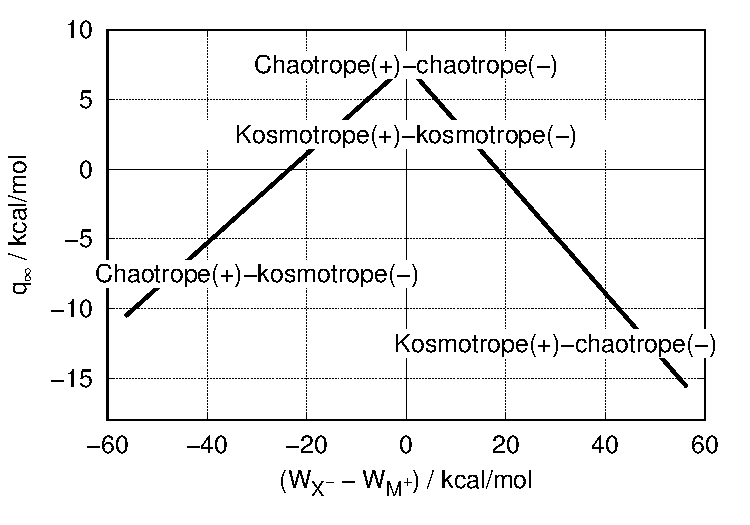
\includegraphics[width=0.98\linewidth]{images/volcano_collins.pdf}
 \end{center}
 \caption[Collins' volcano plot to distinguish similar and dissimilar ion pairs]{\label{fig:collinsvolcano}Ions can be classified as chaotropes (weakly hydrated) or
 kosmotropes (strongly hydrated). This plot illustrates the relationship between the standard heat of solution (at infinite dilution) of crystalline alkali/halide salts and 
 the difference between the absolute heats of hydration of the respective ions. The degree of similarity or dissimilarity between the ions comprising a salt can be qualitatively 
 assessed from its placement into one of four distinct regions (labelled above). Figure recreated from Ref. \cite{collins2007review} (\textcopyright Elsevier Biophysical Chemistry, 
 reprinted with permission) in order to enhance image clarity.}
\end{figure}    

  \section{\label{ch1:sec2:level1}Models of ion solvation}
   Modeling is one of the most effective tools in scientific research. Models unify results, rationalize observations, and grant some level of predictive power under unexplored
   conditions. In this section I briefly review several important advancements in the development of numerical models of the ion solvation problem. 
   
   As discussed above, all of these methods target analytical or numerical solutions to several target properties of the simple ion-into-water scenario: 1) solvation free energies, 
   enthalpies, and entropies of individual ions at infinite dilution, 2) activities and osmotic coefficients, and 3) surface tension increments. Each of these methods make assumptions
   on the nature of ion/solvent and ion/ion interactions. Their shortcomings help us address issues with the underlying physics and so have been instrumental in the evolution of 
   such models over the last century. 
   
   The methods discussed here also share the treatment of solvent as a mathematical continuum in common, meaning no ball-and-stick molecular models are required except for the ion 
   itself. The earliest models covered here ignore the solvent reorientational contributions to the free energy and assume the ion/solvent interactions to be purely electrostatic. 
   Successes and failures of these models will be discussed.
   
   In the second section, I'll explore the corrections considered in modern continuum solvation models. The corrections consider the role of several additional ion and solvent 
   properties which are believed to impart ion specific behavior: dispersion interactions, polarization, charge transfer, cavitation energy (solvophobic effect), ion size (charge 
   density), and surface potentials across chemical interfaces. Extra attention will be paid to the model of Duignan et al. which I believe, despite my criticisms levied against
   it throughout this thesis, is an exceedingly simple and elegant theory of ion solvation. The model is capable of handling ions in dilute solutions, ions moving towards the 
   air/water interface (this is the primary area of disagreement), and ion/ion interactions. 
  
   \subsection{\label{ch1:sec2:level2}The early models}
    Probably the most familiar of these models is the Debye-H\"{u}ckel theory. Debye-H\"{u}ckel theory assumes the interactions between ions to be purely electrostatic (which is
    rigorously true, see the Hellmann-Feynman theorem\cite{politzer2015mathematical}). The solvent is modeled as a dielectric continuum through the dielectric constant and the 
    ion charge density with a Boltzmann distribution. It is only \emph{valid} in the limiting case of low concentrations (<100 mM).
    
%    The starting point for this theory is the Poisson relation,
    
%    \begin{equation}
%        \nabla^{2}\psi(r) = -\frac{\rho(r)}{\epsilon}
%    \end{equation}
    
%    \noindent which defines an electrostatic field $\psi(r)$ due to the charge density $\rho(r)$ in a dielectric medium. The charge density in the Debye-H\"{u}ckel
%    theory is chosen as a Boltzmann distribution,
    
%    \begin{equation}
%        \rho(r) = q_{i}c_{i}^{\infty}\lambda(r)\cdot\exp\left(-\frac{q_{i}\psi(r)}{k_{B}T}\right)
%    \end{equation}
    
%    \noindent where c$_{i}^{\infty}$ is the bulk charge density of an ion with charge q$_{i}$, and $\lambda(r)$ denotes the accessibility of an ion to position $r$ 
%    (typically set to 1, so ignored hereafter). Combining these expressions leads to the Poisson-Boltzmann relation for a collection of charges,
    
%    \begin{equation}
%        \nabla^{2}\psi(r) = -\frac{1}{\epsilon}\sum_{i}c_{i}^{\infty}q_{i}\cdot\exp\left(\frac{q_{i}\psi(r)}{k_{B}T}\right).
%    \end{equation}
 
%    \noindent A position dependent dielectric can be substituted into the expression above as well to mimic chemical interfaces. The equation above is an exact relation for 
%    describing the field of a charge distribution and though solvers do exist, they are typically far slower than other approximate methods.
    
%    Debye and H\"{u}ckel worked out a solution for the electrostatic potential experienced by a spherically symmetric ion \emph{j} suspended in a dielectric medium 
%    for $r$ less than $\alpha$, where $\alpha$ traces the ion surface.
    
%    \begin{equation}
%        \psi(r)_{j} = -\sum_{i}\frac{q_{i}\kappa}{\epsilon\left(1+\kappa\alpha\right)}
%    \end{equation}
    
%    \noindent where $\kappa$ is the inverse Debye length, $\kappa = \sum_{i}\sqrt{\frac{4\pi q_{i}^{2}c_{i}^{\infty}}{k_{B}T\epsilon}}$. The negative of the result of taking
%    half the potential multiplying the charge of ion \emph{j} gives us the excess chemical potential $\mu^{ex}_{j}$. Setting the two sides of the equation equal to one another 
%    and rearranging to solve for $\ln\lambda_{j}$ defines the activity coefficient. Converting from the molar to molal scale allows ionic strengths to be described from this 
%    result as well. Ionic strength can also be expressed in the molar scale, but because the volume change for higher ionic strengths is not strictly additive, it is preferable
%    to use the molal scale in practice.
    
%    The electronic part of the solvation free energy can be derived by substituting the potential above into the Debye charging expression or by solving the integral G = 
%    $\int \frac{U_{e}}{T^{2}} dT$ where $U_{e,j}$ is the electronic potential energy of ion \emph{j} in the field of all the other ions. The equation used in the original
%    paper\cite{debye1923theorie} neglects pressure-volume work under the assumption that the solvent is incompressible.
    
    Debye and H\"{u}ckel expressed the low concentration limit of the free energy of an ion ($\mu_{i}$) in this field as
    
    \begin{equation}
        \mu_{i} = k_{B}T\ln\Lambda_{i}^{3} + k_{B}T\ln c_{i} - \frac{\kappa q_{i}^{2}}{2\epsilon}
    \end{equation}
    
    \noindent where $\lambda$ is the de Broglie thermal wavelength, c\sous{i} the concentration, and the third term is the electrostatic part of the free energy,
    making use of $\kappa^{2} = \frac{4\pi}{\epsilon k_{B}T}\sum_{i}q_{i}^{2}c_{i}$, where $\kappa^{-1}$ is the inverse Debye length. This equation can be rewritten as
    
    \begin{equation}
        \mu_{i} = k_{B}T\ln\Lambda_{i}^{3} + k_{B}T\ln c_{i} + k_{B}T\ln\gamma_{i}
    \end{equation}
    
    \noindent where $\ln\gamma_{i} = -\frac{\kappa q_{i}^{2}}{2\epsilon k_{B}T}$ is the activity coefficient of the i\emph{th} ionic species. This is not accessible to 
    experiment, so the mean activity coefficient is measured instead, giving $\ln\gamma_{\pm} = -\left|q_{+}q_{-}\right|\frac{\kappa}{2\epsilon k_{B}T}$. A plot of the
    $\ln\gamma_{\pm}$ versus $\sqrt{I}$ is linear at low concentrations, where I = $\frac{1}{2}\sum_{i}q_{i}^{2}c_{i}$ and is the (typically) molal ionic strength. That
    is, the approximation of ion-ion interactions as essentially non-interacting, screened point charges is reasonably accurate for low concentrations. At higher 
    concentrations, the limiting expressions break down and exhibit significant deviation from experiment. Application of the Debye-H\"{u}ckel model to osmotic coefficients 
    suffers similar limitations. In a later advancement, Onsager and Samaras extended the model to predict the surface tension of electrolyte solutions\cite{onsager1934surface}.
    
    Aaron Klug, winner of the 1982 Nobel Prize in Chemistry, once quipped that the theory was only applicable to ``slightly dirty water''\cite{parsons2011hofmeister}. This is
    because the model neglects ion specific properties such as the size and shape of the particle(s) and how these change with solvation (see Figure \ref{fig:f-6-r4aa-delrho} 
    for an example of how electron density is drawn to poles which point directly at neighboring solvent molecules). The solvent response is also neglected and is assumed to 
    be uniform throughout space which neglects polarization. Dispersion interactions are also neglected. Debye-H\"{u}ckel theory is still often used to this day in the 
    interpretation of experimental measurements (and so these interpretations also lack these important contributions)\cite{peruzzi2012hofmeister,ribeiro2013salt}.
    
    Some of these features have been introduced in a number of extended models which draw from the Debye-H\"{u}ckel model, see Pitzer ion interaction 
    model\cite{pitzer1977electrolyte} and a very recent iteration of an extended Debye-H\"{u}ckel theory\cite{xiao2011molecular,xiao2015extended} which is applied to ionic liquids. 
    The Derjaguin-Landau-Verwey-Overbeek (DLVO) model for describing the stability of colloidal suspensions has been successfully adapted to address ion solvation as well. 
    This theory incorporates repulsive electrostatic and Lifshitz-like attractive dispersion forces. The electrostatic potential assumes a form very similar to that of the 
    Debye-H\"{u}ckel model. Ionic-dispersion can be modeled by incorporating dynamic polarizabilities from high level electronic structure calculations\cite{parsons2011surface}. 
    Overall, the DLVO model has seen success across a diverse array of fields\cite{parsons2014surface} but is not predictive of Hofmeister effects even with a series of 
    fitting parameters and the addition of terms correcting for hydration and interaction effects not considered in the original theory.

    Evolving around the same time, the Born model of ion solvation is another approximation of the Poisson relation using the Coulomb potential\cite{born1920volumes}. The Born 
    formula is derived from 2\sur{nd} order perturbation theory\cite{tlbbook} and assumes purely electrostatic interactions between the ion and solvent and represents the solvating 
    molecules via a dielectric continuum. It is an expression for the single-ion solvation free energy and takes the form,
    
    \begin{equation}
        \mu^{ex}_{b} = -\frac{N_{A}q^{2}}{8\pi\epsilon_{0}r_{0}}\left(1-\frac{1}{\epsilon_{r}}\right)
    \end{equation}

    \noindent where $\mu^{ex}_{b}$ is the bulk free energy of solvation, bulk meaning without chemical interfaces, q the ion charge, $\epsilon\sous{0}$ the permittivity of free
    space, r\sous{0} an ionic radius (must be spherical; empirically fit), and $\epsilon_{r}$ the dielectric of the solvating medium. The 1 assumes transfer from the gas phase 
    where the dielectric constant is 1. Note that the dependence on the charge in this theory is quadratic -- ions of the same size but opposite charge will have precisely the same 
    solvation free energy. All ions are expected to be repelled from the air/water interface, just as in the Debye-H\"{u}ckel theory\cite{onsager1934surface}. This is, however,
    not the case, as I explain in Chapter \ref{ch1:sec3:level5}. 
    
    The model addresses the finite size of the ions but requires that they be best modeled as an excess charge confined to a spherical cavity. The results can vary quite a bit
    with the selection of ionic radii. However, the theory neglects polarization of, reorganization (cavitation) of, and other interactions with the nearby solvent. The model has 
    been built on just as Debye-H\"{u}ckel theory and forms of the basis of the bulk thermodynamic scale\cite{ashbaugh2008lps,marcus1985book,rashin1985reevaluation} which is 
    discussed in more detail in Chapter \ref{ch1:sec4:level2}. These models refit the crystal radii by increasing the ionic radii\cite{latimer1939freenergy}, selecting vdW radii
    for the vacuum part\cite{stokes1964van}, or simply extend the Born model with additional terms\cite{rashin1985reevaluation}. 
    Additionally, some of the more advanced theoretical models condense down to the Born model under certain conditions\cite{roux1990molecular}. There's good evidence a model 
    like this is perfect for quickly accounting for the distant ion/solvent interactions as only the electrostatic contributions are expected to remain significant beyond the first hydration 
    shells\cite{beck2011local,beck2011lmft,hummer1996,shi2013length}. I even liken some of the results from my own simulations in Chapter \ref{ch6:sec0:level1} to the Born model.
    
    In 1936, Onsager extended the Born model to include polarization interactions between the ion and continuum; however, the model still required a spherical cavity and 
    required knowledge of the ion dipole and polarizability. Others issues include 1) Spherically symmetric ions (our alkali and halide friends) won't solvate in this model. 
    2) The dipole and polarizability of the ion (and nearby solvent) can \emph{change} with 
    solvation\cite{masia2009polarize,masia2013polar,patel2010polarizability,ren2003amoebaion,amoeba,rogers2010ctpolar,silvestrelli1999water}. Figure \ref{fig:dypol} gives an 
    example of this.
    
    Here the dynamic polarizability of the water molecule is plotted for a range of applied frequencies. The water geometries used include the native gas phase one and that when
    the water is complexed with the alkali-halides. In the case of each of the ion-induced geometries, the polarizability at a given frequency is slightly above that of the
    native geometry. This small change enhances the polarization and dispersion interactions. The water geometry when complexed with F\sur{-} distorts to such an extent that
    the polarizability increases from about 1.42 \AA\sur{3} to 1.5 \AA\sur{3}, a far greater change than any of the others. This really does have a significant impact on the
    interactions; the polarization and dispersion energies for this complex are listed in Table \ref{tab:sapt1}. It is this kind of complex chemistry through electronic
    charge rearrangement that continuum models cannot reproduce. However, the effect likely becomes less pronounced with increasing cluster size. According to several studies, 
    the dipole moment of waters in the first shell isn't all that different from the bulk\cite{heuft2003cl,heuft2005f,heuft2005i,krekeler2006density,lightstone2001first}.
    
\begin{figure}
 \begin{center}
  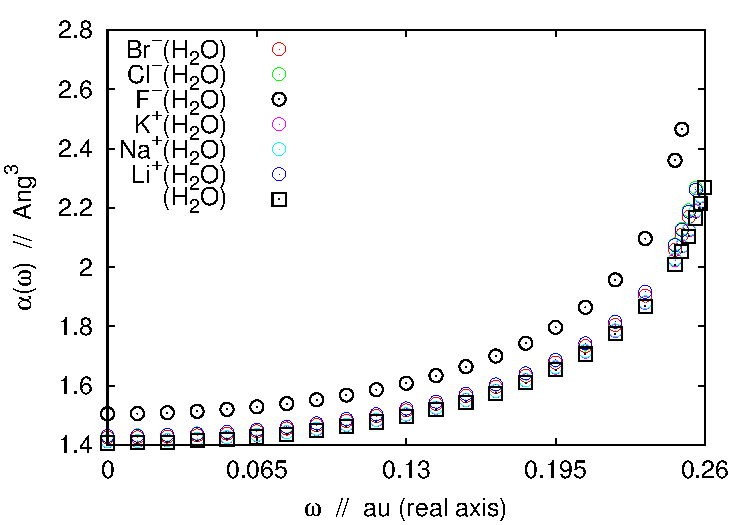
\includegraphics[width=0.98\linewidth]{images/all_polar_data.pdf}
 \end{center}
\caption[Dynamic polarizabilities of water in gas phase and ion-water dimer geometries]{Isotropic dynamic polarizabilities of water in native and ion-induced geometry for a 
range of 0 to 0.26 atomic units applied frequencies. Calculations were performed at the equations-of-motion coupled cluster to double excitations level with the aug-cc-pV5Z 
basis set using NWChem\cite{valiev2010nwchem}. Results are otherwise unpublished but are related to the calculations performed in Chapter \ref{ch3:sec0:level1}.}
\label{fig:dypol}
\end{figure}
    
   \subsection{\label{ch1:sec2:level3}Modern continuum solvation approaches}
    Recall that a solvation free energy model should consider ion/solvent interactions and solvent reorganization in the form of a cavity formation energy (sometimes referred 
    to as the solvophobic effect). Modern continuum solvent models are often built into \emph{ab initio} codes to add approximate solvation effects to molecules handled with 
    electronic structure theory. With the already high computational cost of many of these types of calculations, quality continuum solvation models are in extreme demand. 
    There are many of such methods out there, but the bulk of them are derived from the polarizable continuum model (PCM). This method expresses the solvation free energy in 
    the form,
    
    \begin{equation}\label{pcm}
        \mu^{ex} = \mu^{ex}_{elst} + \mu^{ex}_{disp-repulsive} + \mu^{ex}_{cavity}.
    \end{equation}

    A derivative method called the conductor-like polarizable continuum model (CPCM) and many other electronic structure solvation models involve small rearrangements of or 
    substitutions in the PCM equations. Despite the cavity and dispersion-repulsion terms showing up in Eq. \ref{pcm}, the PCM nor CPCM models handle dispersion or cavity 
    parts of the free energy very well\cite{pcmmodels}. Cavities in these theories are handled as a series of overlapping spheres centered at each of the atoms in the modeled 
    molecule(s). The PCM method is also really expensive with numerous derivatives to compute. CPCM simplifies the procedure greatly and performs very well with high dielectric 
    solvents. The CPCM model was used in a very recent single-ion free energy scale paper\cite{ishikawa2016quantum}.

    Truhlar et al. have developed a general solvation model which uses the full electron density of the molecule(s) to estimate solvent accessible surface area (SASA) and
    atomic surface tensions\cite{marenich2009universal}. These figures are related to the cavitation and dispersion-repulsion energies. Because the model actually attempts to 
    solve for cavitation and dispersion-repulsion interactions, it is often considered the best method for calculating solvation free energies -- the others essentially calculate
    the electrostatic part. The higher quality comes at the expense of computation time though. This model has been used to develop what was once was known as the `gold standard'
    scale in single-ion free energies, enthalpies, and entropies\cite{coe1998cpa1,kelly2006cpa}.

    Other models exist that are similar to those discussed above: COSMO, COSMO-RS, SMX (X=6, 8, 12, etc.), and DESMO\cite{lange2011simple}.
    
    Duignan and coworkers have developed a method recently which also solves for the terms given in Eq. 
    \ref{pcm} and applied it to the determination of single-ion solvation free energies, entropies, partial molar volumes, salt activities, osmotic coefficients, ion/ion potentials
    of mean force upon approach (investigating Collins' law of matching water affinities), and the free energy profile of the hydroxide and hydronium ions approaching the air/water 
    interface\cite{duignan2013continuum1,duignan2013continuum2,duignan2014collins,duignan2014ion,duignan2015hydronium,duignan2016ions}. Electrostatics are handled at the Born 
    level for simplicity but the authors also use the COSMO model (essentially any PCM model will work). Dispersion was handled through determination of the conventional C6, C8,
    and C10 coefficients from dynamic polarizability functions evaluated at the density functional level. They hope to treat dispersion using Green's functions in the future. A 
    simple cavity term is modeled as the product of a solvent-related constant and the excluded volume due to the ion. The volume term takes the distance to the first peak in
    the ion/water (oxygen-atom) radial distribution function from simulation or experiment as input. For ion-ion interactions, this volume excludes regions of overlap between the 
    ions. When the electrostatics are handled with COSMO, an approximate polarization energy is taken into account, else it is left out and suffers the usual difficulties associated 
    with Born solvation. For their study of hydroxide and hydronium approaching the air/water interface a surface potential of +0.13 V was assumed\cite{duignan2015hydronium}. I argue later
    why this assumption is very likely wrong and how their results change if using the potential I estimate in Chapter \ref{ch5:sec0:level1}. Other small errors may be due to the
    use of spherical cavities in the COSMO model for non-spherical ions. 
    
    Their results highlight the special importance of dispersion through $\mu^{ex}_{disp-repulsive}$ but also in the determination of $\mu^{ex}_{elst}$ from the COSMO model. 
    They show in Ref. \cite{duignan2014ion} that the 2\sur{nd} virial coefficient (inputs for both osmotic and activity coefficients -- this is a common extension of the Debye-H\"{u}ckel
    model to higher concentrations) for chaotrope-kosmotrope pairs are especially sensitive to the inclusion of electron correlation in the COSMO energy. The model overall 
    exhibits excellent qualitative agreement with experiment and shows the benefits of hybridizing approaches.
   
    I've reflected on a number of theoretical frameworks for modeling ion interactions with bulk solvent, interfaces, and other ions. These methods are of limited predictive
    value given their oversimplified description of solvation which lacks the granularity of explicit solvation models\cite{jungwirth2006airwat}. Even with extensive parameterization, 
    they struggle to mimic the strong and ion-specific local solvation forces. However, I mentioned (admittedly, in passing) that these models are appropriate for accounting for 
    long-range solvation effects which are almost entirely electrostatic in nature (at least in high dielectric solvents). Therefore, the pursuit is not necessarily in vain. Pairing these
    models with explicit handling of the first solvation shell(s) could lead to significant advances in the efficiency and accuracy of hybrid electronic structure/continuum
    approaches. This may also allow researchers to forego the use of periodic boundaries in simulation and simulate proper clusters free from artificial forces due to the
    boundary conditions. The quasichemical theory of solutions which I discuss in Chapter \ref{ch2:sec4:level4} and implement in Chapter \ref{ch6:sec0:level1} measures parts of 
    the free energy as the work to solvate a cavity of considerable size. Dipoles and quadrupoles forming at this junction can interact over a significant distance and may produce
    spurious and unaccounted errors when interacting with its image in a neighboring cell\cite{remsing2014lp}.
   
    Regardless, it is critical to stress that ion solvation is an inherently quantum mechanical problem due to the strong electric field around the ion and the importance of localized, 
    mutually polarizing, non-electrostatic forces, and other as yet undisclosed contributions.
    
  \section{\label{ch1:sec3:level1}Ion solvation is a quantum mechanical problem}
   This section motivates the use of electronic structure theory in the characterization of ion/ion and ion/solvent interactions. Though it is also instructive to point out that 
   ``well-parameterized classical models can capture important aspects of specific ion hydration, including high resolution single-ion thermodynamic quantities''\cite{pollard2016review}. 
   Indeed, the size of and timescales of simulations run today are virtually impossible to carry out at the electronic scale. So where does the need for very costly quantum chemistry
   come into play? Our successes in modeling ion solvation to spectroscopic and/or thermochemical accuracy can be used to train simpler models which can in turn be used to address
   matters requiring many atoms or long timescales.
   
   So what is going on in these inner shells that continuum models cannot reproduce (even in an \emph{average} sense)? In short, \emph{a lot}. There's a surprisingly large number
   of things to discuss on this matter so I'll break things down into a few categories (by no means an exhaustive list): 1) spectroscopic and theoretical evidences of chemical 
   character in the closest shells, 2) dynamical effects, particularly on solvent exchange between the inner shells, 3) nuclear quantum effects, 4) ions at interfaces, and 5) 
   some additional thoughts on atomistic modeling of non-electrostatic contributions for some perspective on how far we've come and the limitations of many existing force fields.
   
  \subsection{\label{ch1:sec3:level2}Chemical character of ion solvation}
   First, I re-establish the fact that monovalent ionic effects are limited to the first or second solvation shell. Markovich et al. measured the photoelectron spectra of 
   sequentially solvated ion/water clusters\cite{markovich1994photoelectron}. They measured the binding energy of the valence electrons of Cl\sur{-}, Br\sur{-}, and I\sur{-} ions
   with increasing cluster size, relating the change in the binding energy between subsequent cluster sizes to a stabilization energy. This figure was monitored with increasing
   cluster size to determine the size of the first solvation shell. The authors found this energy largely stabilized by a cluster size of \emph{n} = 6. Interestingly, each of the
   spectra reflected an increase of over 3 eV in the binding energy associated with solvation. A later study by Kurahashi et al. determined these values more accurately, with all
   of the respective binding energies increasing\cite{kurahashi2014photoelectron}. These authors observed that the change in the highest occupied molecular orbital (HOMO) binding 
   energy for the solvated water molecule decreases $\sim$1.3 eV relative to the gas phase water molecule. A redshift in other spectral features of water are observed as well and are
   linked in Ref. \cite{fransson2016x} to the formation of the hydrogen bonding network in bulk water. Intermediate these studies was one from Winter et al.\cite{winter2005electron}.
   The spectra in this paper are argued to have been superseded by those of Ref. \cite{kurahashi2014photoelectron}, but these authors also attempted to compute the binding energies
   using a combination of continuum and explicit particle methods. They found that continuum methods performed well for cations because solvent reorganization could be largely 
   neglected (the transition is from +1 to +2 charge), while for anions the continuum methods struggled (transition is from -1 to $\pm$0 charge). In water, the dipole orientation
   around a neutral cavity most resembles that of a cation\cite{wipff1999tatb,wipff2000tatb,wipff2001tatb,hummer1996}, leading to the poor comparison. A later study embedded partially
   solvated anion/water clusters in the same model and achieved significantly improved agreement with experiment\cite{dolgounitcheva2014microsolvation}. A separate study postulated
   that the neutral state of a particularly difficult case for band assignment in the spectrum of F\sur{-}/water more resembles F\sur{-}/H\sous{2}O\sur{+}\cite{canuto2010delocalized}, 
   likely owing to the large proton affinity of F\sur{-}\cite{kim2002bigall}. In a review by Seidel et al.\cite{seidel2016valence}, the vertical detachment energies (the binding 
   energies assuming no change in solute or solvent structure) are reported to correlate very well with the UV charge-transfer-to-solvent (CTTS) energy, even getting the Hofmeister 
   ordering of monovalent anions largely correct. Some of these authors recently reported on a new method for probing solvent-separated, solvent-shared, and contact ion pairs
   related to Collins' law of matching water affinities\cite{unger2016first}.
   
   It has been a longstanding goal across many fields to describe the dynamics of the solvated electron which is the simplest form of electron transfer reaction and so is a surrogate
   for understanding more complex chemistry. It is also believed to play a role in radiation induced damage of DNA\cite{coons2016hydrated}. Iodide is the most commonly used electron
   donor since it is relatively easy to excite and the simple nature of the neutral atom with no vibrational degrees of freedom reduces the number of variables to contend with in the 
   measurements\cite{kothe2015charge}. The solvated electron is generated by exciting the iodide valence orbitals to produce an I\sur{0}-e\sur{-} state (the nature of which is poorly
   understood)\cite{kothe2015charge}. The intermediate survives a reported 1-2 picoseconds before generating the solvated electron which relaxes after about 100-500 
   femtoseconds\cite{kothe2015charge}. Spectra of this sort have been produced both experimentally and theoretically for the halide series and even the sodium
   anion\cite{barthel2000direct,bradforth2002excited,galamba2009electronic,kim2000smallall,kim2002bigall,kloepfer1998femtosecond,lehr1999electron}. 
   
   But there's growing evidence that you don't need to excite the valence electrons of anions to see a portion of the excess charge spill out onto the 
   solvent\cite{angelina2013cov,attah2015structure,cordoba2011ctinhbonds,hynes2000cthalides,hynes2008ctnitrate,kim1999bigf,kim2000smallall,kim2002bigall,klein2005solutesolventct,lee2012ctice,mccoy2006prywaterf,mo2006polctqmmm,patel2010polarizability,rogers2010ctpolar,soniat2012ct,sarkar2013cthalideohraman,soniat2014ct_surf,rick2016polct}.
   Many of these studies relate intermolecular charge transfer (also known as charge displacement) to spectral shifts in IR or Raman stretching frequencies of the solvating water(s)\cite{xiong2010lowest}. 
   Another pair of studies (and the experimental and theoretical references therein) discuss modeling of the vibrational spectra for water when complexed with an 
   ion\cite{kamarchik2010quantum,puniyan2016theoretical}. This too is a very localized effect and can be so strong an influence that in the case of F\sur{-} and water, the ion is 
   often said to act as though it is ``prying apart'' the molecule\cite{collins2007review,mccoy2006prywaterf}. In a study by Choudhuri et al., the authors monitor the vibrational 
   frequency of the O-D stretch over the course of a simulation as the molecule diffuses away from F\sur{-}\cite{choudhuri2012first}. There is about a 200 cm\sur{-1} blueshift
   in the frequency as the molecule returns to the bulk. In a follow-up studies on Br\sur{-} and I\sur{-}, the authors noted that the O-D stretching mode actually decreased as the water
   diffused into the bulk\cite{karmakar2013first,karmakar2015water}. Diffusion coefficients in the first shell were also found to be greater than in the bulk, consistent with discussion
   above on the ``tumbling'' of waters around the alkali-halides measured with NMR\cite{karmakar2015water}. The use of heavy water minimizes the impact of nuclear quantum effects with 
   hydrogens.
   
   Using the quantum theory of atoms in molecules\cite{bader1990book}, I looked into this idea of F\sur{-} somehow ``prying apart'' the water molecule from the perspective of changes 
   in the electron density Laplacian (curvature) as a function of ion/water separation as in Ref. \cite{espinosa}. In Figure \ref{fig:laprho}, I show a previously unpublished plot
   of the curvature of the electron density measured at the junction between the halide anions and a bound water molecule. I monitor this quantity over a range of separations and compare 
   between two levels 
   of theory. In the atoms in molecules theory, a positive curvature indicates ionic character, while negative indicates covalent character. While not negative in value, it is very 
   interesting to note that the equilibrium geometry of the F\sur{-}/H\sous{2}O dimer falls on the part of the curve where the curvature becomes less positive with decreasing distance, 
   while both Cl\sur{-} and Br\sur{-} exhibit the opposite behavior. In Ref. \cite{espinosa}, this behavior is likened to a closed shell (electrostatic) interaction with emerging 
   covalent character. It's easy to rationalize that F\sur{-} forms stronger hydrogen bonds with water than the other halides. Kim et al. point out the high electronegativity and large 
   proton affinity of F\sur{-} relative to the other halides\cite{kim2000smallall}. But does the unique location of F\sur{-} on the Laplacian curve necessarily support this covalent
   narrative? It's possible, but we mustn't jump to conclusions. At the least I think it implies the exchange of density between the fragments is more fluid, but then again this behavior
   is difficult to characterize because there is no unique way to carve individual atoms out of a molecular system. Why is this definition of an ``atom'' better than another? That's a
   discussion beyond the scope of this thesis. Safe to say, Bader's theory does not impress some\cite{emptor} -- probably one of the most scathing reviews of anything I've ever seen.
   
   In spite of the difficulties associated with charge partitioning, partial charge transfer is believed to \emph{symmetrize} the first solvation shells by promoting internal ion 
   solvation over surface solvation\cite{rogers2010ctpolar,soniat2012ct}. Though induction is typically taken to include intramolecular polarization and intermolecular charge transfer, 
   high polarizability has been linked in several studies with increased solvation asymmetry (surface binding)\cite{carignano1997polarizable,dang1993molecular,herce2005surface,ohrn2007many,perera1992structure}. 
   Reconciliation may be found in an explanation that charge transfer reduces the excess charge on the ion, effectively making it harder and less polarizable. 
   
   Rick and coworkers have also argued that the cumulative charge transfer from the bulk to the interface leads
   to the apparent negative surface charge of air bubbles or oil droplets suspended in water\cite{vacha2011oil,soniat2014ct_surf,takahashi2005zeta}. However, the calculated excess 
   surface charge falls well short of those back-converted from experimental $\zeta$-potentials (about 60-150x smaller). The alternative hypothesis is OH\sur{-} adsorption at the 
   interface which is a \emph{highly} contentious topic I'll address later.
   
   The sheer number and diversity of structures reflected in many of the above studies and others such as Refs. \cite{ivanov2014stabilization,kemp2005theoretical,lambrecht2011exploring,lambrecht2012refined} 
   and those used in Chapter \ref{ch3:sec0:level1} very likely places an approximate description of local structure beyond the reach of continuum models as well.
   
\begin{figure}
 \begin{center}
  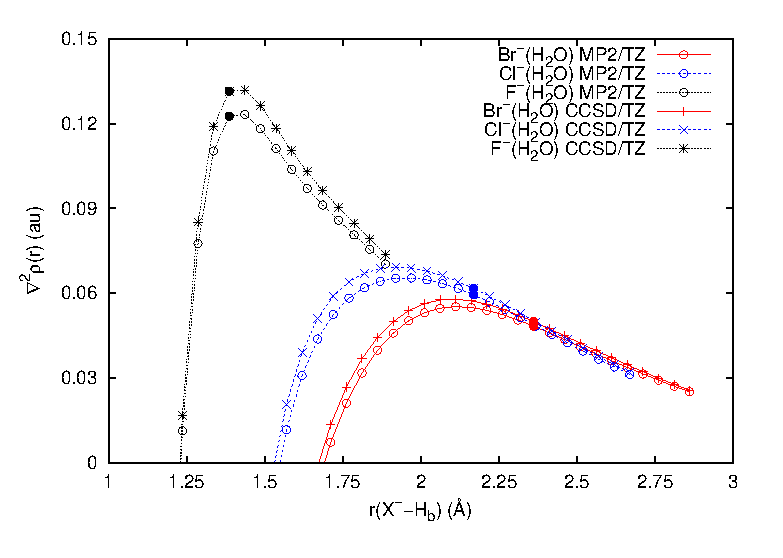
\includegraphics[width=0.98\linewidth]{images/laprho_v_distH.eps}
 \end{center}
\caption[Electron density curvature in halide/water dimers versus separation]{Laplacian (curvature) of the electron density in halide/water dimers measured at the bond critical point
linking the ion and water. A positive value indicates that density is not shared across the point, while a negative value denotes the opposite. According to Ref. \cite{espinosa}, the 
position of F\sur{-} on this curve is unique in that it coincides with the emergence of covalent character in the `bond.' Results are otherwise unpublished but are related to the 
calculations performed in Chapter \ref{ch3:sec0:level1}.}
\label{fig:laprho}
\end{figure}   
  
  \subsection{\label{ch1:sec3:level3}Temporal evolution of the solvation shell}
   Perhaps one of the most difficult aspects of ion solvation and possibly the best argument for molecular resolution is the \emph{softness} of the hydration shell conferred through
   the finite time of ion/solvent interactions, diffusion, and exchange between the first and second solvation shell. The earlier results of Heuft and Meijer suggest the first hydration 
   shell is rather \emph{hard} around F\sur{-} and Cl\sur{-} -- in this sense meaning sharply cut off from the rest of the solution\cite{heuft2003cl,heuft2005f}. Though they find the
   solvation shell around I\sur{-} to be rather unstructured with rapid exchange between shells\cite{heuft2005i}. Karmakar et al. in their series of studies on halide ion solvation 
   also addressed the diffusion coefficients of ion-bound waters, the lifetime of hydrogen-bonds, and dynamics of water reorientation in the first 
   shell\cite{choudhuri2012first,karmakar2015water}. The dynamics of first shell waters was found to fall into three distinct timescales: short-time relaxation dynamics ($\sim$100 fs), 
   lifetime of the X\sur{\pm}$\cdot\cdot\cdot$H bond (F\sur{-} ($\sim$7.5 ps) > Cl\sur{-} ($\sim$3 ps) $\approx$ Br\sur{-} ($\sim$3-4 ps) > I\sur{-} ($\sim$2-3 ps) > H\sous{2}O 
   ($\sim$1-2 ps)\cite{bankura2014structure,ojha2015ultrafast}). The somewhat labile nature of the coordination shell is supported also by the work of Laage and 
   Hynes\cite{laage2007reorientional}. A somewhat dated study by Kozi{\'n}ski et al. estimated the lifetime of the hydrogen bond between water and CN\sur{-} to be about 2.9 
   ps\cite{kozinski2007vibrational}. Interestingly these changes come with no discernible change in the dipole moments of the waters between the first and second 
   shell\cite{heuft2003cl,heuft2005f,heuft2005i,krekeler2006density}.

   Water residence times also differ significantly across the halide series (F\sur{-} ($\sim$26 ps) > Cl\sur{-} ($\sim$20 ps) $\approx$ Br\sur{-} ($\sim$20 ps) > I\sur{-} ($\sim$14-16 ps)). 
   As shown by Heuft et al., the solvation shell of the ion when undergoing solvent exchange will take on unique characteristics not observed for low energy conformers used to parameterize 
   continuum and simple all-atom models\cite{heuft2003cl,heuft2005f,heuft2005i}. F\sur{-}, for example, will take on a short lived hexahydrate coordination sphere before returning one of
   the waters to the bulk\cite{heuft2005f}. The inherent flexibility in the coordination number can only be reasonably approximated with an all-atom model and then again only 
   \emph{accurately} with electronic structure resolution. Residence times are also critically important in understanding the dynamics of solvation around proteins\cite{pal2002biological}
   which can be modified by the presence of electrolytes (and hence the Hofmeister series).
   
   These results also stress the importance of including dispersion effects in density functional modeling of hydrogen bonding dynamics in electrolyte 
   solutions\cite{bankura2013hydration,bankura2015systematic}. However, some care must be taken to be sure the corrected functional doesn't over/under structure water, as is common.
   Recent simulations also highlight the critical importance of dispersion in modeling the first shell of Na\sur{+} and K\sur{+} to accurately determine coordination numbers from the 
   integral of the radial distribution function\cite{bankura2014hydration}. A systematic review of the challenges ion solvation pose for density functional theory can be found in 
   Ref. \cite{soniat2015dispersion}.
   
  \subsection{\label{ch1:sec3:level4}Nuclear quantum effects}
   Much of the simulation work discussed above was done with heavy water, but why? As the proverb goes, ``when it rains it pours.'' Extending beyond the usual difficulties in 
   describing the electronic wave function, the small mass of the proton means nuclear quantum effects play an important role in hydrogen bonded systems.
   Nuclear quantum effects (NQEs) are purported to increase the mobility of both H\sur{+}\cite{marx2000solvated} and OH\sur{-}\cite{tuckerman2002nature}, which may be important in
   proton shuttling along membranes and hydrophobic surfaces\cite{zhang2012water}. NQEs are also likely responsible for a number of anomalous behaviors in liquid water and in 
   ice\cite{pamuk2012anomalous}. 
   
   Nuclear effects are generally thought to occur in hydrogen bonds through two competing modes 1) proton sharing through a stretching mode
   (HO$\cdot\cdot\cdot$H$\cdot\cdot\cdot$O$\cdot\cdot\cdot$H\sous{2}) and 2) distortions in the bond due to rotation of the participating molecules\cite{ceriotti2016nuclear}.
   As a general rule of thumb, nuclear effects weaken weak hydrogen bonding interactions and strengthen stronger ones\cite{ceriotti2016nuclear,guo2016nuclear}. You might think this 
   makes NQEs more important for anion solvation -- but it has actually been found to be more important for Li\sur{+} than F\sur{-} due to the competing effects discussed 
   above\cite{wilkins2015nuclear}. Suzuki et al. have also found that NQEs in small F\sur{-}/water clusters led to elongation of the hydrogen bond distance\cite{kawashima2013ab}. 
   Wang et al. observed similar behavior in small Cl\sur{-}/water clusters.
   
   These effects can be included for both quantum and classical descriptions of electrons. Including NQEs generally improves the quality of simulations across a broad range of 
   temperatures\cite{vega2010heat}. In conventional \emph{ab initio} dynamics a 30--50 K increase in the temperature has been found to mimic NQEs and corrects the radial 
   distribution function (rdf) of liquid water at 300 K (simulation temperature is 330--350 K) and slightly decreases the overall structuring (lower peak in 
   rdf)\cite{morrone2008nuclear}. However, this is a questionable approximation\cite{weber2010communication}. Additional influences of NQEs are addressed in a recent
   review\cite{ceriotti2016nuclear}.

  \subsection{\label{ch1:sec3:level5}Ion adsorption at the air/water interface}
   Ion adsorption at the air/water interface is a relatively recent discovery. For quite some time it was believed that all ions were repelled from the interface because 1)
   the surface tension of water increases with the addition of most inorganic salts predicting a negative surface excess by the Gibbs adsorption isotherm and 2) the primitive
   dielectric models predict that ions solvated in a higher dielectric medium are repelled from the interface due to an image charge force. The air/water interface was believed 
   to be ion-free and relatively inert\cite{ishiyama2014theoretical,jungwirth2006airwat}. This all changed with Hu et al.\cite{hu1995reactive} who noticed that the kinetics of Cl\sous{2} and 
   Br\sous{2} uptake in solutions of NaI and NaBr did not fit the rate predicted by a bulk-phase reaction mechanism (X\sous{2} + Y\sur{-} $\rightarrow$ XY + X\sur{-}). The 
   authors inferred significant surfactant behavior of Br\sur{-} and I\sur{-} as Y\sur{-} to fit their model to their experimental measurements. Since then, research into the 
   surface activities of inorganic ions and the acid/base chemistry of the water surface has become wildly popular.
   
   Cheng et al., Netz et al., and Ou et al. have found strong correlation between anion affinity for the air/water interface and ion radius\cite{cheng2006experimental,netz2009ionsinterfaces,ou2016molecular}. 
   Researchers more commonly ascribe surface propensity to 
   polarizability\cite{jungwirth2002airwat,jungwirth2006airwat,pegram2006partitioning,pegram2007hofmeister,petersen2005adsorption,petersen2006nature,wick2007effect}.
   Polarizability (or an especially large dipole on the waters in nonpolarizable models) was found to be a critical factor in determining whether this behavior would be seen
   from molecular dynamics trajectories\cite{stuart1996effects}. However, the role of polarization in polarizable force fields such as AMOEBA may be overestimated somewhat, 
   exaggerating the role polarization may play here\cite{rogers2010ctpolar}. There may be several competing effects also including surface capillary waves, desolvation, cavity 
   formation, and the surface potential across the air/water boundary\cite{ayse2012,ben2016interfaces,rane2016understanding}. 
   
   Surface affinity appears to also change with the counterion in solution\cite{cheng2012ambient,hua2014cation,tissot2015cation}. The ordering of ions in the double layer can
   switch when the anion is strongly kosmotropic and the depth of the region of ion accumulation/depletion at the interface can extend to more than a nanometer into the solution\cite{brown2015ion}. 
   However, the region of enhanced ion density relative to the bulk is more commonly limited to about half that distance. This is based on density profiles of the ionic species 
   extracted from molecular dynamics simulations and also the anion/cation ratios probed at various depths by high-pressure photoelectron spectroscopy\cite{jungwirth2006airwat}. 
   The density profiles and spectra also show that the net charge density profile over the interfacial region produces a negative surface excess. The depleted layer a few water 
   diameters deep more than makes up for the surface active layer(s) above it, an illustration of this is given in Ref. \cite{jungwirth2006airwat}. 
   
   Hua et al. have also shown that the interface can be depolarized at sufficiently high concentrations of surface active ions; the authors used 1.7 M perchlorate in this case\cite{hua2013surface}. 
   Depolarizing the interface with an applied voltage while monitoring relative surface excesses may be used to approximate the contact/surface potential essential to the
   establishment of an absolute single-ion thermodynamic scale\cite{conboy1997shg_tatb}.

   While the surface activity of some ions is well-established, there are still some lingering issues with quantifying the enhancement (see Refs. 253--256 in Ref. \cite{bjorneholm2016water})
   due to discrepancies between X-ray methods, sum-frequency (SFG) and second harmonic generation (SHG) spectroscopies, and theoretical approaches. Adsorption of hydronium 
   or hydroxide ions at the interface remains an extremely contentious topic of research, however. Hydroxide adsorption at the interface is suspected because 1) the 
   $\zeta$-potential in neat water is negative as mentioned previously, 2) the surface tension of a freshly formed air/water interface relaxes from 80--100 mN/m to 73 mN/m 
   in about 1 ms (about the same time required for OH\sur{-} buildup due to autolysis and diffusion); competing mechanisms occur on ps (too fast) and s (too slow) timescales\cite{liu2012surface},
   3) other anionic and/or fatty acid impurities are not observed at the air/water interface in SFG/SHG experiments\cite{jena2012surface}, 4) the isoelectric point of the air/water
   interface is at pH 2.5--4\cite{beattie2014surfacid,buch2007surfacid,liu2012surface,mishra2012surfacid}, and 5) the surface tension of water is largely pH-independent from 
   pH 4--13. This last point does not necessarily point to one ion over the other making an appearance at the interface (as noted in Ref. \cite{jungwirth2015comment}), but 
   demonstrates the robust nature of the surface charge, strengthening the conclusions generated from other studies. 
   
   Theoretical studies and SFG/SHG experiments typically predict hydronium adsorption at the interface\cite{buch2007surfacid,mucha2005unified,petersen2008liquid,tse2015propensity,willow2011nh4+}.
   A notable exception is a study by Mundy et al. which found a small $\sim$0.6 kcal/mol attraction of OH\sur{-} to the air/water interface\cite{mundy2009hydroxide}. The 
   free energy profile of H\sous{3}O\sur{+} is more often shown to have a minimum near the interface, while the OH\sur{-} profile is purely repulsive. This is interpreted to
   reflect the loss of water contacts by OH\sur{-} and a favorable enthalpic contribution through exclusion of H\sous{3}O\sur{+} from the bulk\cite{tse2015propensity}. However, 
   a study by Brorsen et al. made the interesting observation that hydronium did not prefer surface solvation when the ion and water were modeled at the \emph{ab initio} level, 
   but did when the water was handled with the TIP5P water model\cite{brorsen2014surface}. This is a 5-point classical point charge model which is known to have almost no 
   surface potential contribution\cite{remsing2014lp}. The surface potential is believed to play a role in ion adsorption at interfaces\cite{ayse2012,duignan2015hydronium}.
   The surface potential I derive in Chapter \ref{ch5:sec0:level1} acts at about $\frac{1}{2}$ its full value near the interface and if included in the study of Tse et al. in Ref. 
   \cite{tse2015propensity} reverses their prediction. Adsorption of the OH\sur{-} ion is selected over H\sous{3}O\sur{+} by $\sim$4--6 kcal/mol, similar to that discussed 
   in the conclusions of Ref. \cite{liu2012surface}. This difference corresponds to a $\sim$10\sur{4} preference for OH\sur{-}. This is consistent with the pH needed to 
   neutralize the surface of water.
   
   There are also several complicating factors with surface sensitive spectroscopies which are in need of resolution: 1) the signal can be convoluted by poorly understood 
   quadrupolar or bulk solvent contributions\cite{carrier2016ionsatowinterface,kundu2016bend}, 2) the probe depth is poorly characterized and appears to be able to change with
   ionic strength from about 1 nm to over 1 $\mu$m\cite{gonella2016second}, 3) the signal which is thought to measure surface adsorption does not necessarily translate back to
   propensity\cite{carrier2016ionsatowinterface}, and 4) the OH\sur{-} may (weakly) or may not be visible to SFG/SHG\cite{imamura2014molecular,mishra2012surfacid}. These are
   important concerns to address considering that SFG/SHG are also used to probe structure of the air/water, oil/water, and other non-aqueous solvent
   interfaces (e.g., directionality of the O-H bond: pointing into vapor phase or into bulk?)\cite{conboy1997shg_tatb,luo2015electrobreak,wang2016surface}. Issues with 
   theoretical approaches are typically related to the small size of simulations and the poor performance of classical force fields for this type of work\cite{beattie2014surfacid}.
   
   See Refs. \cite{bjorneholm2016water,bonn2015molecular,ishiyama2014theoretical,wang2016surface} for additional reviews on interfacial effects and surface sensitive 
   spectroscopies and Ref. \cite{agmon2016protons} for a recent survey of literature related to the ongoing debate about H\sous{3}O\sur{+}/OH\sur{-} surface affinity.
   
  \subsection{\label{ch1:sec3:level6}Additional comments on modeling non-electrostatic forces}
   Polarizable force fields are hit and miss with over-polarization being a pretty severe problem in classical models\cite{vdS2011surfacepref} in comparison with more realistic 
   quantum models\cite{baer2011toward}. Another concern is whether the model should make use of full gas phase or reduced condensed phase ion polarizabilities\cite{masia2009polarize,patel2010polarizability}.
   The popular AMOEBA force field has seen some refinement in the parameters over the years to combat these 
   issues\cite{laury2015revised,ren2003amoeba,ren2003amoebaion,amoeba,ponder2010znamoeba,wang2013systematic} but still over-polarizes anions. This can be corrected by variation 
   of a damping parameter employed in the self-consistent polarization calculation\cite{pollard2014cpa1}. However the adjustment necessarily distorts the solvation structure and 
   thermodynamic quantities without full re-parameterization. In the calculations I perform in Chapter \ref{ch5:sec0:level1}, the F\sur{-}/water peak in the radial distribution
   function is pushed about 0.25 \AA~beyond that when using the default model parameters. This was a fortuitous change for us however as I discuss in that chapter.
   
   Additionally, the AMOEBA assigned polarizability of the particles is static when I have shown previously that it can in fact change. The effect may not be as pronounced in 
   water where the dipoles of waters in the first shell may not differ drastically from those more distant from the ion, but this is not the case in every solvent\cite{ayse2016ecpc}, 
   also see Chapter \ref{ch4:sec0:level1}. The model of Steve Rick and coworkers reviewed in Ref. \cite{rick2016polct} I think represents the state of the art in force field 
   modeling. It incorporates two major improvements over AMOEBA in particular. 1) Polarization is handled using a Drude oscillator which adjusts the polarizability dynamically
   based on the environment and takes gas phase polarizabilities as input and 2) the model incorporates a simple and efficient description of charge transfer. Stuart and Berne 
   used a similar model, concluding that the larger dipole moment of these water models as compared to nonpolarizable ones made for a more accurate representation of both the
   dielectric and dynamic properties of liquid water\cite{stuart1996effects}. Fortunately, despite the deficiencies in polarizable force field models, they are often 
   qualitatively correct and have proven exceedingly useful in addressing selective adsorption of ions at the air/water interface.

   The van der Waals (vdW) potential in classical force fields, meanwhile, is a kind of mathematical Frankenstein composed of dispersion, exchange repulsion, surface potential
   effects, and corrections for all manner of uncategorized errors necessary to produce a better fit to a desired property. Fits of interaction parameters may be done against a
   dizzying array of experimental variables\cite{nezbeda2016recent} and sometimes the parameters of cations and anions are fit to different experimental quantities, best 
   exemplified in Ref. \cite{netz2009}. Nezbeda et al. have published a recent review on the difficulties of force field development especially as it pertains to the theoretical
   prediction of electrolyte solubility\cite{nezbeda2016recent}. The authors (and I) believe some standardization is desperately needed. My work in Chapters \ref{ch5:sec0:level1} 
   and \ref{ch6:sec0:level1} defines and characterizes a separate surface potential effect which also can serve to clean up the vdW potential in \emph{all} force fields a bit. 
   These papers also provide a road map for relating simulated quantities to experiment. Surface potential effects and single-ion thermodynamics are addressed in the next section.

  \section{\label{ch1:sec4:level1}Surface potential effects on the solvation of ions}
   Earlier I argued that the determination of an accurate single-ion thermodynamic scale was essential in our pursuit to finally begin to unravel the specific ion effects. What
   follows is a summary of the state of affairs in establishing such scales in aqueous and two energy storage related media, namely ethylene and propylene carbonate.

  \subsection{\label{ch1:sec4:level2}The single-ion scale}
   Solvation properties of neutral particles can be uniquely determined through experimental methods as long as an accurate equilibrium constant between gas and solution phase
   partitioning can be established. This applies also to ion \emph{pairs} wherein one ion neutralizes the net charge of the other. Solubility measurements can also be used to 
   establish solvation properties though the lattice energy of the salt must be removed to convert solution properties to solvation ones\cite{peruzzi2015solvation}, 
   see the representative thermodynamic cycle in Figure \ref{fig:thermocycle}. A list of lattice energies is found in Ref. \cite{marcus2012ions} on page 33. 

% trim .... left, bottom, right, top
\begin{figure}
 \begin{center}
  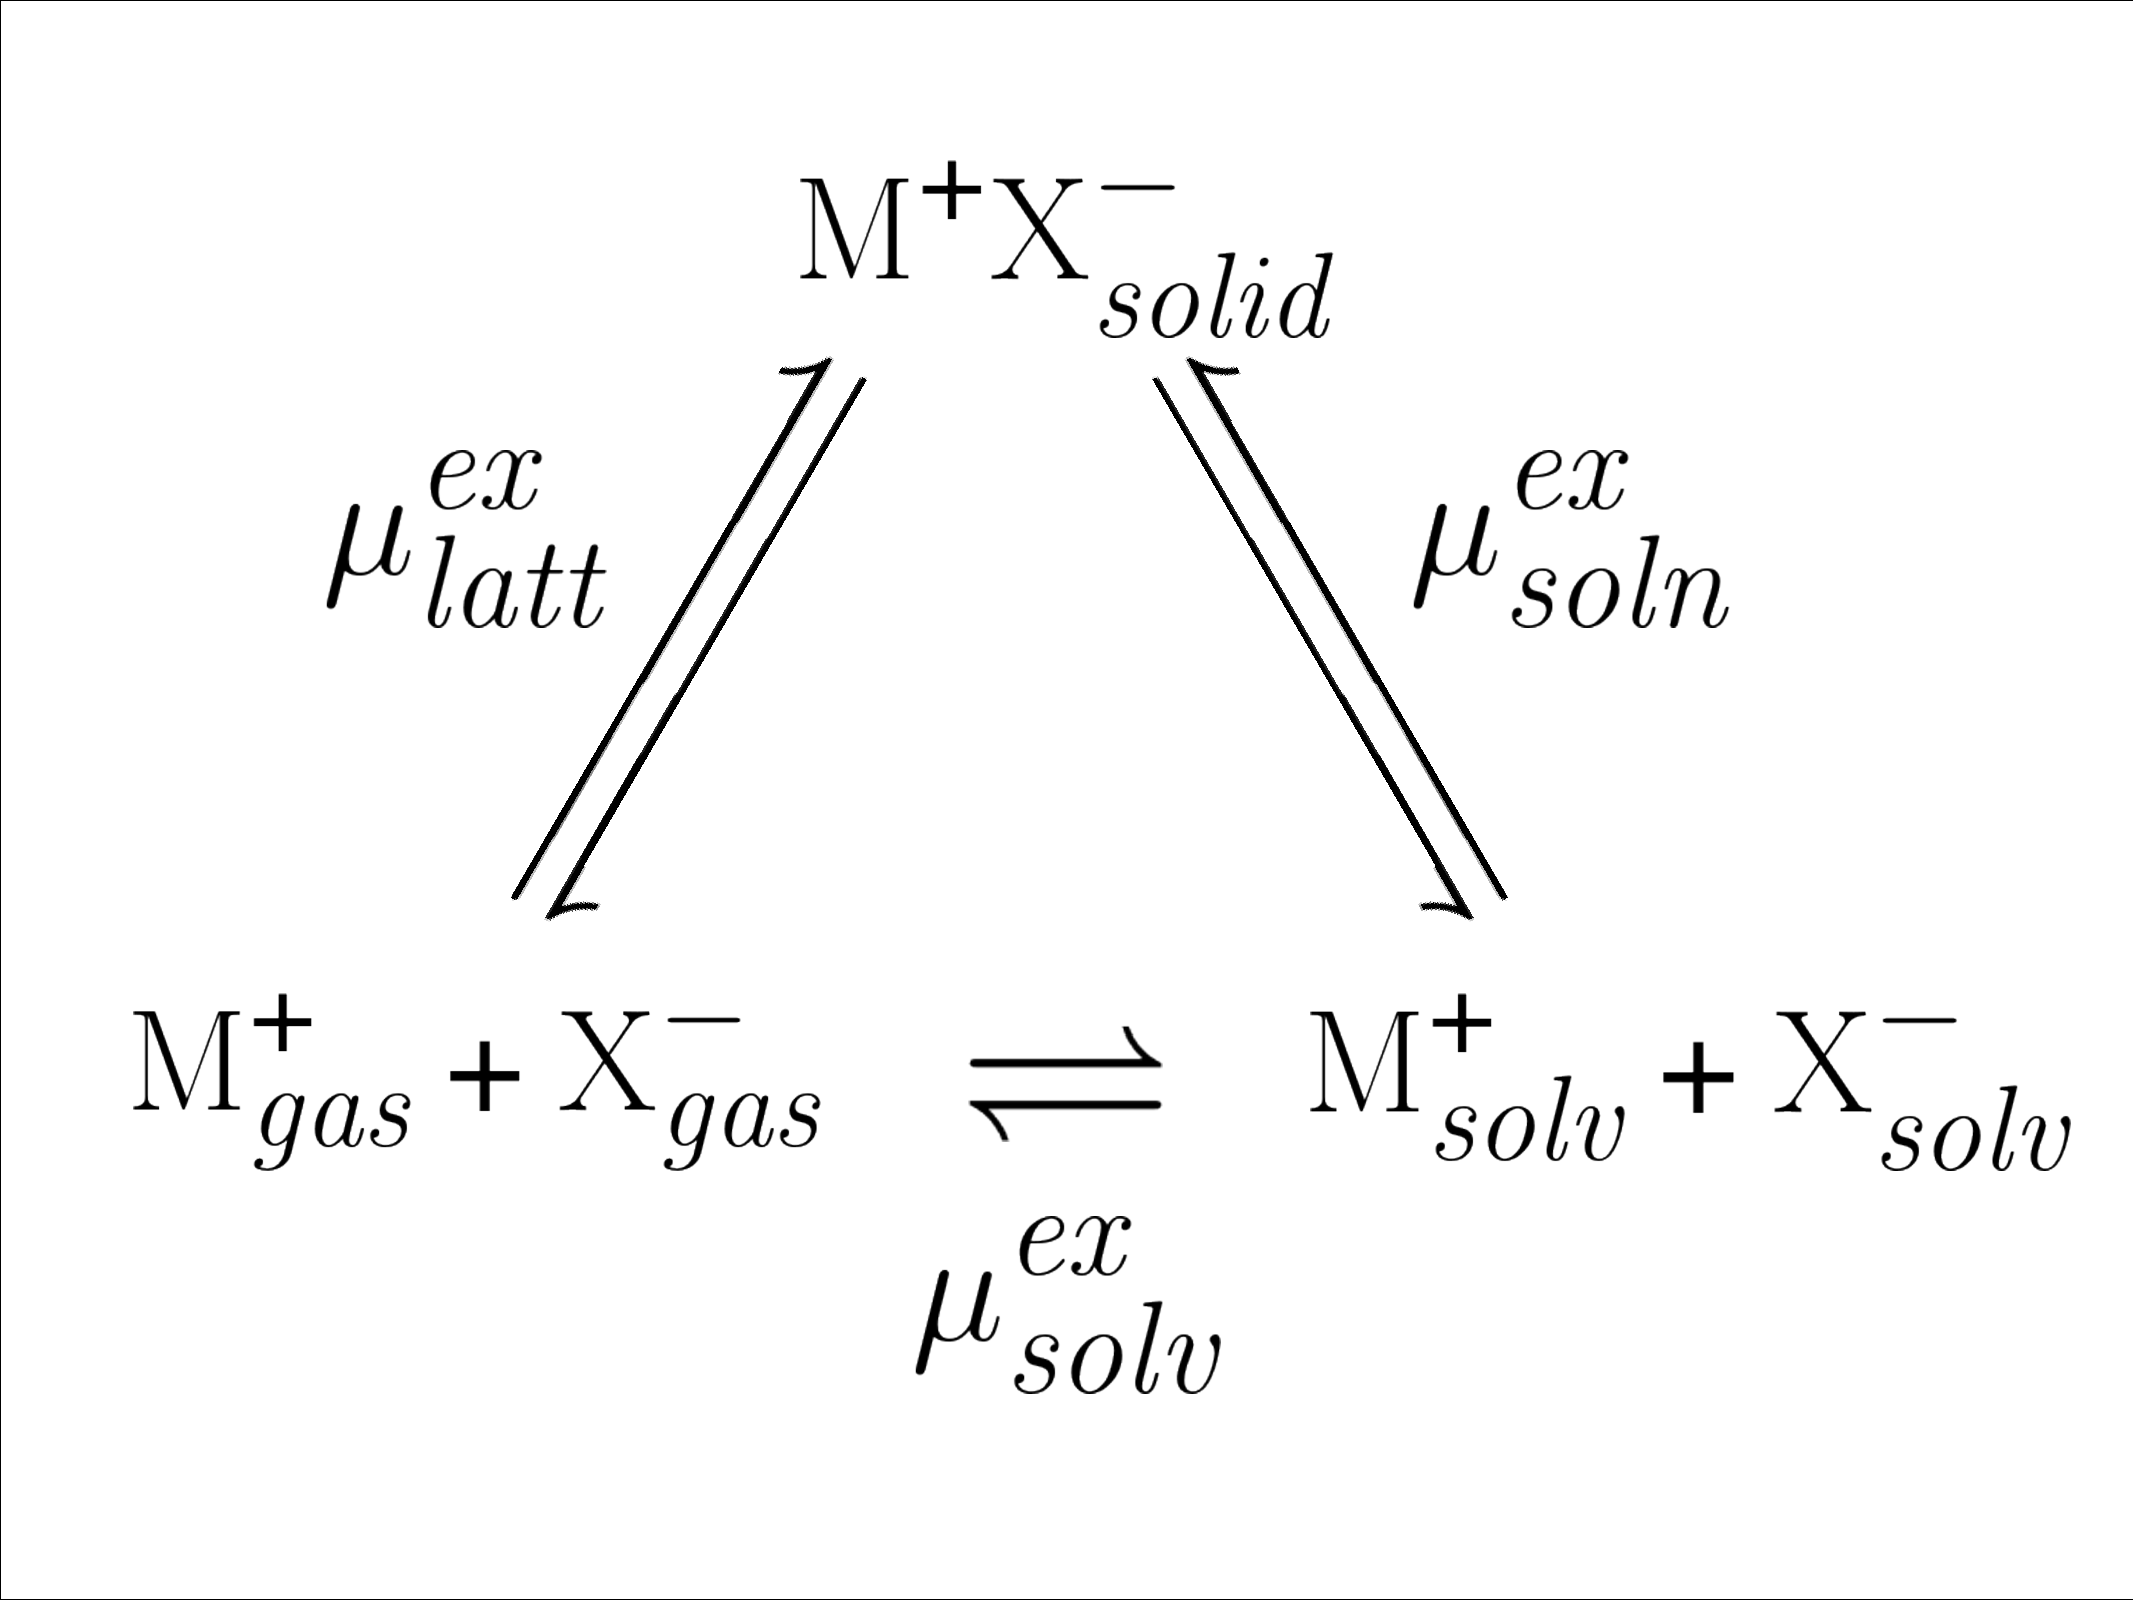
\includegraphics[width=0.98\linewidth,trim=0.2cm 2.2cm 0.2cm 0.2cm,clip=true]{images/thermocycle.pdf}
  \caption[Schematic of the thermodynamic cycle]{A thermodynamic cycle relates the lattice free energy, solution free energy, and solvation free energy through a series of 
  transitions/transfers.}
  \label{fig:thermocycle}
 \end{center} 
\end{figure}     
   
   The solvation free energy and related properties are a specific case of transfer free energy from vapor into solution rather than between two solutions. More generally, 
   transfer experiments can be conducted in mutually saturated solvents that are in contact with one another or in the pure solvent. The choice can often lead to very different 
   results as the more hydrophilic ions tend to coextract with residual waters into the non-aqueous phase\cite{rose2009, darvas2011, darvas2013}. Electrochemical
   methods can be used as well\cite{gomer1977experimental,randles1956real}. More recently advanced mass spectrometry setups have been used to determine sequential hydration
   enthalpies and based on my results from Chapter \ref{ch5:sec0:level1} may be able to establish the most accurate thermodynamic scale to date\cite{wheeler2015hydration,bard2014electroanalytical}.
   A list of pair free energies for alkali/halide salts is shown in Table 6 of Ref. \cite{lamoureux2006absolute}. There is typically very little variation in the pair
   solvation properties between different measurements and these are known to high accuracy\cite{ren2003amoebaion}. 
   
   The solvation free energy for a salt is very simple,
   
   \begin{equation}\label{eq:pairmu}
       \mu^{ex}_{pair} = \mu^{ex}_{P,b} + \mu^{ex}_{N,b},
   \end{equation}

   \noindent so long as we don't try to separate the contribution made by each ion individually. Once we try to do that, the best we can come up with is the \emph{conventional}
   scale where everything is measured relative to the proton,
   
   \begin{equation}
     \mu_N^{ex,con} =  \mu^{ex}_{N} + \mu^{ex}_{\mathrm{H}^+} = \mu^{ex}_{N,b} + \mu^{ex}_{\mathrm{H}^+,b}
     \label{eq:conv1}
   \end{equation}

   \noindent for a negatively charged ion and

   \begin{equation}
     \mu_P^{ex,con} =  \mu^{ex}_{P} - \mu^{ex}_{\mathrm{H}^+} = \mu^{ex}_{P,b} - \mu^{ex}_{\mathrm{H}^+,b}
     \label{eq:conv2}
   \end{equation}   
   
   \noindent for a positive one. This is because with the exception of mass spectrometry, no other experimental method is able to make measurements on isolated charges. Even
   then, these studies are limited to the determination of sequential hydration enthalpies for clusters extending just beyond the first shell. It's more common to split
   bulk thermodynamic and electrochemical measurements using an extrathermodynamic assumption to solve for the proton quantities and thus all others through Eqns. \ref{eq:conv1}
   and \ref{eq:conv2}. Some of the more cited of these are reviewed below.
  
   Another problem in the determination of a single-ion scale is the fact that dragging charges across solution interfaces also incurs a contribution from the electrostatic 
   potential associated with the interface. This is often called the surface potential, phase potential, or contact potential\cite{lamoureux2006absolute,pratt1992contact}. 
   Pioneering minds like Gibbs and Guggenheim long ago ruled this pursuit out concluding potential shifts experienced by single ions moving across interfaces are not 
   thermodynamically measurable\cite{gibbs1,guggenheim28,guggenheim-td}.
   
   Nevertheless, the real electrochemical solvation free energy for a single ion is expressed as\cite{aquaincognita2014,pratt1992contact,fawcett,beck2013sp},
   
  \begin{equation} 
    \mu_X^{ex} = \mu_{X,b}^{ex} + q\phi_{np}
    \label{eq:echemmu1}
  \end{equation}

  \noindent where $\mu_{X,b}^{ex}$ is the bulk hydration free energy (that includes all interactions of the ion with water except for the surface potential 
  contribution). $\mu_{X,b}^{ex}$ is also called the \emph{intrinsic} free energy\cite{hunenberger2011sp} and $\mu_X^{ex}$ the \emph{real} free energy. Similar
  nomenclature is extended to the hydration enthalpy which is
  
  \begin{equation}
    h_X^{ex} = h_{X,b}^{ex} + q\phi_{np} - qT\left(\frac{\partial \phi_{np}}{\partial T}\right)_P
    \label{eq:echemh1}
  \end{equation}

  \noindent and the hydration entropy\cite{lynden1997hydrophobic} is

  \begin{equation}
    s_X^{ex} = s_{X,b}^{ex} - q\left(\frac{\partial \phi_{np}}{\partial T}\right)_P.
    \label{eq:echem1}
  \end{equation}

   \noindent The enthalpy and entropy add a new term which corresponds to the temperature derivative of the surface potential. The enthalpy also contains a contribution
   made by the surface potential itself, while the entropy does not. The surface potential contributions cancel out in Eqns. \ref{eq:pairmu}--\ref{eq:conv2} leading to the
   excellent agreement among the various methods for pair and conventional free energies and the like. These figures become less agreeable when the pair quantities are 
   divided into their respective single-ion scales, see Figure 2 in Ref. \cite{lamoureux2006absolute}. With this in mind, let's review some of the more commonly cited 
   extrathermodynamic assumptions.
   
   \begin{itemize}
       \item Marcus scale\cite{marcus1985book} using the method of Halliwell and Nyburg\cite{halliwell1963enthalpy} for the proton enthalpy and Conway's bulk proton solvation
       entropy\cite{conway1978evaluation}. The values are -254.3 kcal/mol, -261.5 kcal/mol, and -24.0 cal/mol-K for the free energy, enthalpy, and entropy respectively.
       \item Born model with adjusted radii (Latimer-Pitzer-Slansky)\cite{ashbaugh2008lps,latimer1939freenergy}, giving identical results to the Marcus method.
       \item Assuming equal solvation entropies between H\sur{+} and OH\sur{-} (s\sursous{ex}{H\sur{+}} = s\sursous{ex}{OH\sur{-}})\cite{schmid2000blkfe}. The proton 
        quantities are -251.4 kcal/mol, -257.6 kcal/mol, and -20.7 cal/mol-K for the free energy, enthalpy, and entropy respectively.
       \item Assuming very large, ligand-screened, hydrophobic ions of opposite charge  have the same solvation properties in \emph{every} solvent 
       (tetraphenylarsonium/tetraphenylborate, TA\sur{+}/TB\sur{-})\cite{marcus1987tatb}. These results are slightly shifted from those of Marcus above. The hydration enthalpy
       of the proton is -263.6 $\pm$ 1.7 kcal/mol. The Conway entropy is assumed again\cite{conway1978evaluation}. The hydration free energy is then -256.4 kcal/mol.
       \item The extrapolation of gas phase, sequential hydration properties to the bulk via the cluster pair approximation\cite{coe1998cpa1,coe2001cpa2,coe2002cpa3,kelly2006cpa}. 
       The values here are very different from those above: -265.9 kcal/mol, -274.9 kcal/mol, and -30.0 cal/mol-K for the free energy, enthalpy, and entropy respectively.
       More recent re-evaluations with the method have led to a new set of recommended values: -265.3 kcal/mol, -275.3 kcal/mol, and -33.3 cal/mol-K\cite{donald2010expand_cpa}.
   \end{itemize}
   
   The last result here very clearly differs from the others, but it is most certainly not the only one in that range, more are listed in Ref. \cite{ishikawa2016quantum}. This 
   difference extends to the other ions when these proton values are inputted into the \emph{conventional} free energy scale above (again, see Figure 2 in Ref. \cite{lamoureux2006absolute}). 
   Previous efforts have determined that all but the last of the listed approaches above \textbf{excludes} the charge-dependent, linear surface potential term in the free 
   energy\cite{asthagiri2003absolute,ashbaugh2008lps,beck2013sp,shi2013length}. I refer to these values as the ``bulk'' quantities from Eqns. \ref{eq:echemmu1} -- \ref{eq:echem1}. 
   Could the surface potential in Eqns. \ref{eq:echemmu1} and \ref{eq:echemh1} be the piece that links these scales together and explains why they appear shifted from one another? 
   What even is this surface potential contribution? These questions are central to my work in Chapter \ref{ch5:sec0:level1}.

  \subsection{\label{ch1:sec4:level3}The air/water surface potential}
   In reference to Figure \ref{fig:potqct}, $\phi\sous{sp}$ is the total surface potential across the air/water interface and $\phi\sous{lp}$ is the imaginary inner interface 
   across the solvent/solute boundary where the electrostatic potential differs from that of the bulk solvent. I'll refer to $\phi\sous{lp}$ as the local potential, a
   recent study has also identified this potential\cite{remsing2016role}. $\phi\sous{sp}$ has been characterized by simple point charge models, electrochemical experiments, 
   density functional calculations, and complex electron holography measurements with values ranging from -1 to nearly +4 V\cite{leung2009sp_mag}. The origin of this tremendous 
   spread was beautifully illustrated by Kathmann et al.\cite{kathmann2011sp}. To summarize, density functional calculations and high energy electron holographic measurements
   have access to interrogate the full electron density while electrochemical measurements samples from the intermolecular density which leads to a smaller observed potential 
   jump relative to the vacuum. Contributions to this potential were found to be almost entirely due to molecular quadrupoles. A large cancellation of $\phi\sous{sp}$ occurs 
   crossing the solvent/cavity interface as $\phi\sous{lp}$ is of similar magnitude but opposite sign. Their sum produces the net potential ($\phi\sous{np}$), which is reduced
   from $\phi\sous{sp}$ and $\phi\sous{lp}$ by about an order of magnitude\cite{harder2008origin,kathmann2011sp,beck2013sp,remsing2014lp}. The shift in free energies due to interfacial 
   potentials has also been observed in several studies\cite{lamoureux2006absolute,ashbaugh2008lps,beck2013sp}.
   
\begin{figure}
 \begin{center}
  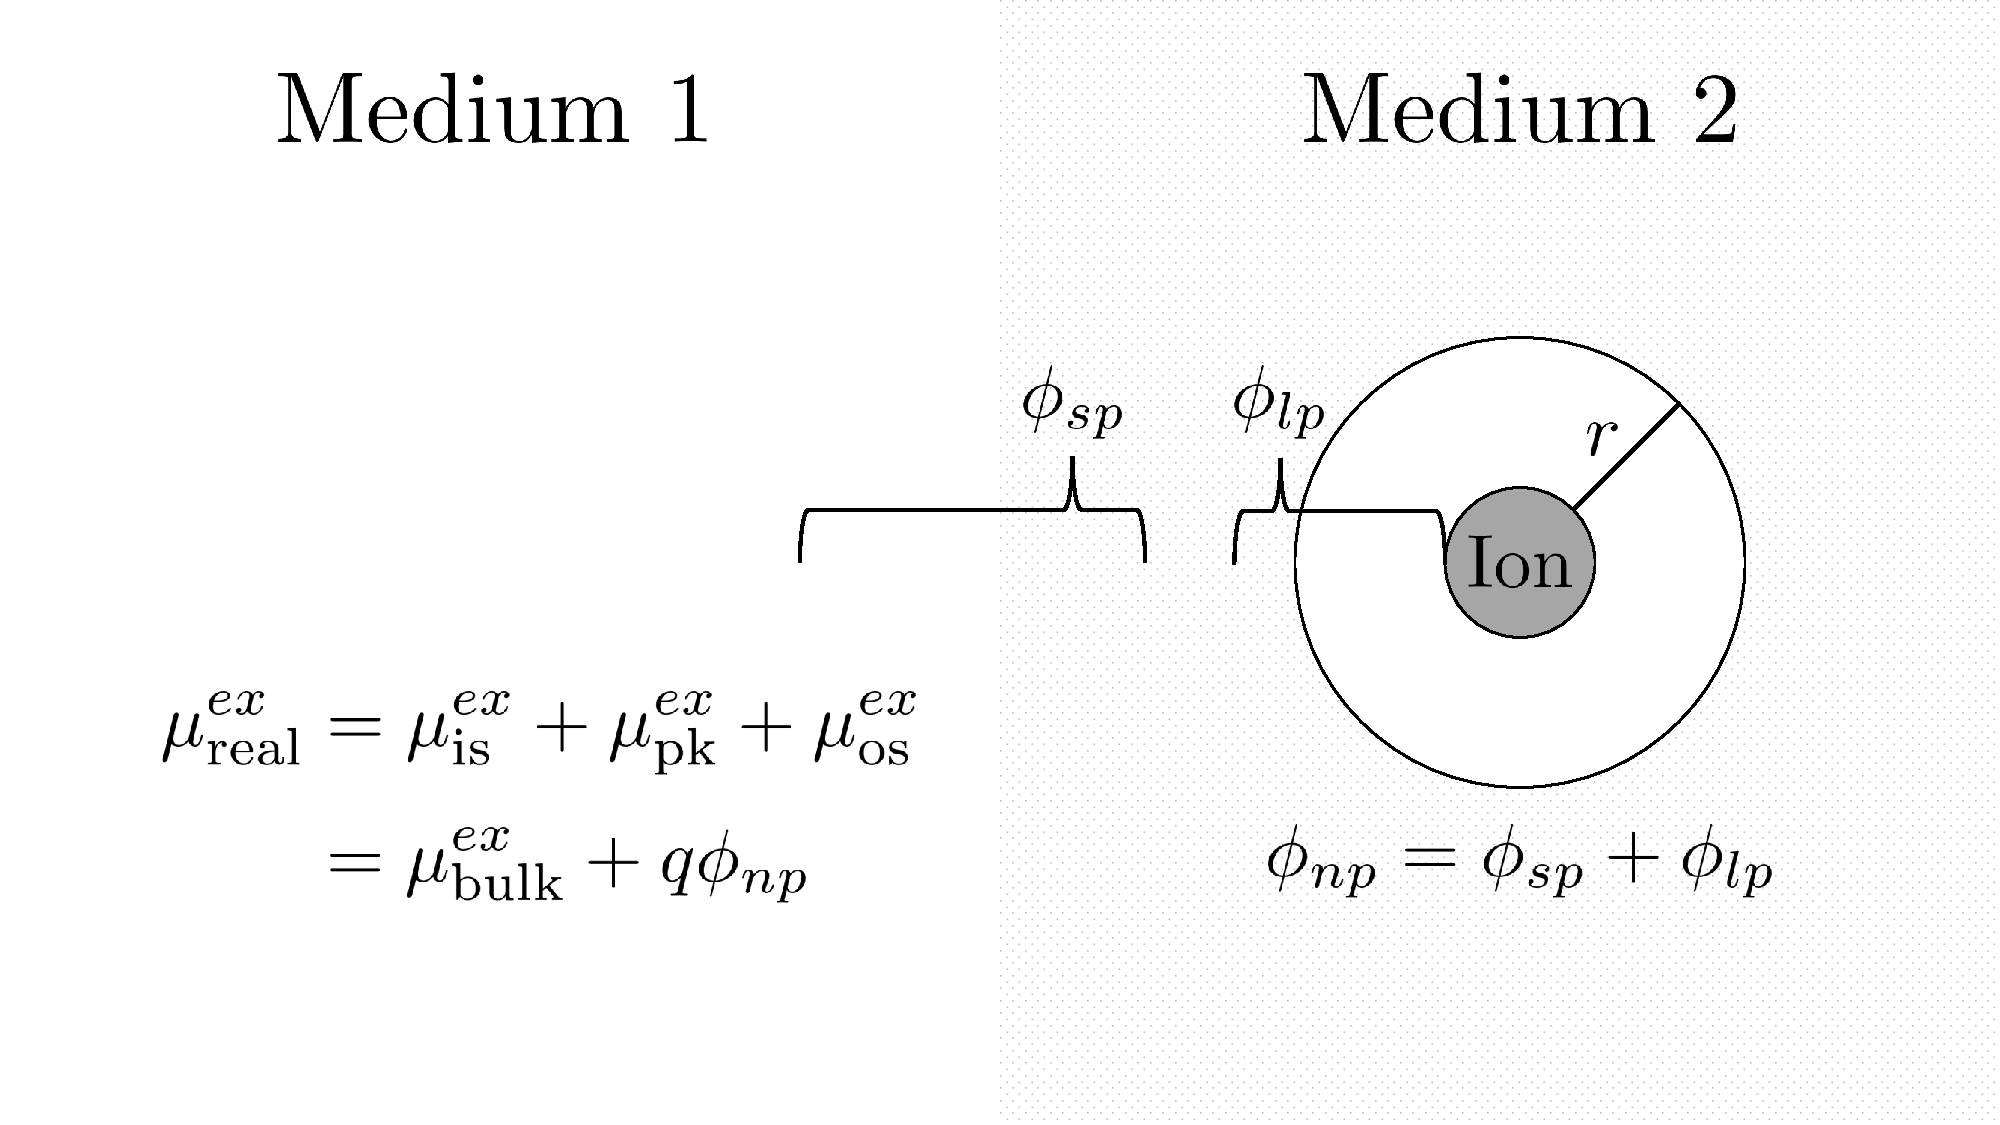
\includegraphics[width=0.98\linewidth]{images/qct_sp.pdf}
  \caption[Illustration of interfacial potentials]{Figure showing interfacial potential contributions across two distinct media to single-ion solvation free energy with 
  quasichemical partitioning. The net and local potentials can be measured as the average electrostatic potential felt by the ion solvated in medium 2 (i.e., water) in 
  a large exclusion zone with radius \emph{r}. For these calculations, the `ion' is modeled only as a spectator to define a location for the cavity. It bears no charge 
  nor interacts with the solvent in any way other than to exclude it. If medium 1 is vacuum, the potential measured in this way is the net potential. If medium 1 is 
  excluded and medium 2 is modeled in periodic boundaries then the local potential is measured. Neither potential is considered in a consistent (or correct) way in 
  molecular modeling using classical force fields and represents a serious error.}
  \label{fig:potqct}
 \end{center} 
\end{figure}  

   Point charge models yield results similar to electrochemical measurements, though there is no such simple explanation of why that is exactly. It is interesting to 
   note that applying a Gaussian smearing function to a point charge model has been seen to somewhat increase the measured surface potential suggesting that the 
   distribution of charge over all space may be important to correctly modeling surface chemistry\cite{pratt1988gaussian_sp}. Estimates of $\phi\sous{np}$ from classical 
   charge distributions or quantum estimates are very nearly identical though the magnitudes of $\phi\sous{sp}$ and $\phi\sous{lp}$ are very different and even of 
   opposite sign\cite{leung2009sp_mag,beck2013sp,remsing2014lp,warren2007hydration}. 
   
   The similarity between the surface potentials measured by electrochemical probes and $\phi\sous{np}$ led me to refer to the net potential as an electrochemical 
   surface potential. This is the average potential experienced by an ion crossing the air/water boundary and it shifts the free energy and enthalpy of solvation by 
   an amount equal to q$\phi\sous{np}$, where q is the ion charge. $\phi\sous{np}$, it's been argued\cite{ayse2012}, may play a role in anion adsorption to the air/water
   interface\cite{jungwirth2002airwat,jungwirth2006airwat}. The basicity of surface waters with an isoelectric point in the neighborhood of 
   2-4\cite{buch2007surfacid,mishra2012surfacid,beattie2014surfacid}, a shift in $\mu\sursous{ex}{H\sur{+}}$ from the bulk of +5.46 kcal/mol, also reflects the influence
   of $\phi\sous{np}$ (predicted to be half as large at the surface)\cite{ayse2012,duignan2015hydronium}. Surface effects could play a role in atmospheric 
   chemistry\cite{buch2007surfacid}. This is especially true of acid-base chemistry where the interface has been found to increase dissociation of carbonic acid
   relative to the bulk\cite{galib2014oceanacid,galib2014hbondingcarbonic} while it was noted by Baer et al. that both HCl and HNO\sous{3} are more likely to remain
   undissociated at the interface\cite{baer2014investigation}. In follow-up work, the authors found that HNO\sous{3} was about 20\% less dissociated in the interfacial 
   layers than in bulk solution even in nearly 8 M solutions\cite{lewis2011does}.

   H\"{u}nenberger and Reif\cite{hunenberger2011sp} have argued +0.13 V, the average of literature values, a reasonable estimate of $\phi\sous{np}$, which
   I contest is actually a composite of estimates of various $\phi\sous{np}$'s and $\phi\sous{sp}$'s and so the average has no physical meaning. However, this figure was
   recently adopted into a continuum model of ion solvation\cite{duignan2014ion} and to addressing the surface activity of the hydronium (H\sous{3}O\sur{+}) and hydroxide (OH\sur{-}) 
   ions\cite{duignan2015hydronium}. The free energies reported by Duignan et al.\cite{duignan2015hydronium} were observed to be particularly sensitive to the ion radius 
   used with the COSMO solvation model. An initial set of parameters produced a free energy (which includes the effect of the surface potential in the electrostatic term, 
   see Eqn. 8, of -167.5 k\sous{B}T for H\sous{3}O\sur{+} and -194.9 k\sous{B}T for OH\sur{-} at 293.15 K. In a second set, the ion radius was fit to reproduce
   experimental values with the proper standard state correction\cite{camaioni2005stdstcorr}. The radius of H\sous{3}O\sur{+} is decreased while OH\sur{-} is increased.
   The corrections adjust the electrostatic part of the free energy and reproduce the expected -189.2 k\sous{B}T and -179.4 k\sous{B}T hydration free energies for H\sous{3}O\sur{+} 
   and OH\sur{-}, respectively\cite{camaioni2005stdstcorr}. 

   The authors have adjusted the ion size to make up for what they attributed to errors in computing the ion-dependent part of the free energy but an 
   alternative explanation is that they've used the wrong surface potential. The shifts in the free energies reported by Duignan et al. are similar to the difference
   between H\"{u}nenberger and Reif's average value and the one I calculate in Chapter \ref{ch5:sec0:level1}. The charge dependent correction is another clue
   that the surface potential may be involved. But the point of this exercise is very simple: using the wrong surface potential can lead to an incorrect
   interpretation of ion solvation where interfacial effects are expected to be important. See also batteries and supercapacitors where performance is linked
   with the partitioning of ions between solid electrodes and some media (can be gas, water, organic solvent, or solid)\cite{li2015solid,schutter2015toward}.

  \section{\label{ch1:sec5:level1}Ion solvation in energy storage cyclic carbonate solvents}
   Non-aqueous environments provide a similar challenge, though there have been far fewer experiments conducted than in water. The scope of this discussion will
   be limited to carbonate solvents used in modern energy storage devices such as the Li-ion battery and supercapacitors, see Ref. \cite{goodenough2013li} for a 
   wonderful review of Li-ion technology and advancements over the years. 
   
   The Li-ion battery (LIB) is found in virtually all mobile devices (e.g., cell phones, laptops, tablets, etc.). They are also used in hybrid or all-electric 
   vehicles and have been used to power and warm our most intrepid explorers (i.e., the Mars rovers)\cite{ratnakumar2006li}. The Li-ion battery cell is composed 
   of an anode, cathode, electrolyte, and a separator. The anode is typically a carbon-based material like graphite, the cathode is a lithium metal oxide, and the
   electrolyte is a non-aqueous aprotic solvent\cite{voelker2014trace}. The separator is permeable to Li-ions and keeps the two electrodes from making contact. 
   Charging the cell with an externally supplied voltage (i.e., plugging in your device) pushes Li-ions and electrons from the cathode to the anode (electrons flow
   through an external circuit). These particles migrate back to the cathode when discharging. 
   
   Repeated cycling between charging and discharging leads to performance degradation over time through a series of chemical and/or thermal pathways. These 
   include oxidation of the electrolyte by the cathode, reduction of the electrolyte by the anode, and thermal decomposition of the electrolyte or electrodes\cite{voelker2014trace}. 
   However, some initial decomposition of the electrolyte is desired. This forms an ion permeable but nonconducting film at the electrolyte/electrode interface which
   prevents further decomposition of the electrolyte (called the solid/electrolyte interphase, SEI). Over time, the oxidative and reductive stresses of discharging
   and recharging lead to additional degradation products which not only affect battery performance but also introduce a number of safety concerns. These issues are 
   borne out of the fact that carbonate solvents have very low flash points compared to their expected operating temperature. The battery also requires a regularizing 
   mechanism to ensure the output falls between a finely specified range appropriate for the application and especially avoids overcharging (voltages greater 
   than 4.2 V)\cite{ohsaki2005overcharge,ratnakumar2006li}. Exceeding this voltage leads to rapid decomposition of the electrolyte, breakdown of the protective film, 
   evolution of CO\sous{2} at high pressure, and thermal instability resulting in irreversible damage to the cell\cite{voelker2014trace}.
   
   Suggested areas of improvement to the Li-ion battery design are delineated in a recent article by Brown et al.\cite{brown2015ion}. They are ``1) finding 
   electrodes that provide the highest energy densities, 2) developing an optimized electrolyte with the high ionic conductivity and stability at high 
   potential/temperature and 3) the appropriate solid electrode/electrolyte interphase (SEI).'' These improvements address safety concerns, capacity issues,
   small voltage range, relatively rapid degradation (even if the cell is never used), and lengthy recharge times which have limited the adoption of Li-ion 
   technology in the electrification of automobiles and other transport vehicles. The greater energy demands of the future (primarily from non-OECD countries) 
   also place a great emphasis on evolving the modern battery\cite{eia}. As does the use of storage technologies to supplement fluctuations in the output of a
   global energy grid increasingly reliant on renewable energy sources.
   
   Much of the focus to date has been on improving the materials of the cathode and anode to push the chemical potentials as far apart as possible, though under the
   new conditions the electrolyte is likely to become the bottleneck to further improvements\cite{husch2015large}. Computational screening has proven a useful tool 
   in screening potential electrolytes to limit the chemical space necessary to explore further with experiment. This reduces both cost and time of 
   development\cite{husch2015large,korth2015,schutter2015toward}. However, screening efforts thus far have focused on a number of simple to compute properties
   which makes use of continuum solvation models for the measurement of solvation free energies (a crucial factor in determining the effectiveness of an electrolyte 
   for shuttling ions between the electrodes\cite{xu2010differentiating,xu2012li}). The resulting free energies lack appropriate handling of the first solvation shell 
   and the surface potential of the solvent -- each critical to the accurate assessment of ion transport in these solvents. Additionally, it has been discussed in the
   literature that additives can greatly influence the cycling efficiency of the cell even at part per million concentrations, including in low temperature 
   conditions\cite{aurbach1992behaviour,zhang2002effect}. This reduces the relevance of studying bulk solvation properties in pure solvents as secondary and tertiary
   solvent effects are likely to significantly affect ion transport and SIE properties\cite{aurbach1992behaviour}. 
   
   It is also believed that the coordination structure around the Li\sur{+} is essential to the formation and structure of the SEI\cite{smith2014x}, though this is still
   poorly understood even in existing carbonate-based electrolytes. Thermodynamic data is almost non-existent in these solvents as well. Despite it being generally accepted 
   that both ethylene (EC) and propylene (PC) carbonate solvents tetrahedrally solvate the Li\sur{+}, there is no consensus in the literature on this point. Most experimental 
   and theoretical predictions place the coordination number in the neighborhood of \emph{n} = 4--5, with Raman intensity experiments and theoretical predictions on the lower 
   end of that range\cite{allen2014combined,bhatt2010interaction,bhatt2012density,borodin2006litfsi,borodin2009quantum,ganesh2011accurate,hyodo1989raman1,hyodo1989raman2,leung2010liion,li1999theoretical,morita1998raman,nie2013role,soetens1998molecular,takeuchi2009ion}
   while X-ray absorption, neutron scattering, and conductivity data predict 4.5 PC molecules to each Li\sur{+}\cite{kameda2007solvation,kondo2000conductivity,smith2014x}. 
   Smith et al. found that a classical polarizable force field underestimated (the same one used in Refs. \cite{borodin2006litfsi,borodin2009quantum}) the coordination 
   number relative to experiment\cite{smith2014x}. Bogle et al. found the coordination number in EC to be as high as 5.69\cite{bogle2013understanding}. The largest value yet
   was determined by Castriota et al. who estimated a Li/EC coordination number of $\sim$7 in 1 M solutions of LiClO\sous{4}\cite{castriota2003temperature}. My work in
   Chapter \ref{ch4:sec0:level1} also makes an estimate of the coordination number from density functional based simulation.
   
   A universal coordination number of 4 was assumed in the computational part of a recent study by Brown et al. which predicted the differences in binding energy between 
   Li\sur{+}-1s and Cl-2p\sous{3/2} (in ClO\sursous{-}{4}) core states in ethylene carbonate, dimethyl carbonate, (3:1) dimethyl carbonate to ethylene carbonate mixtures, 
   and dimethyl sulfoxide\cite{brown2015ion}. A comparison with near ambient pressure photoemission with liquid jet X-ray spectroscopy established that ethylene carbonate 
   more strongly solvates Li\sur{+} than the other carbonates\cite{brown2015ion}. This finding is consistent with a study by Yang et al. which established that \sur{13}C 
   chemical shifts of EC were more strongly shifted upon complexation with Li\sur{+} than other carbonate solvents\cite{yang2010investigation}. A similar conclusion was drawn 
   for the binding of EC relative to PC\cite{aurbach1992behaviour}. This strong binding contrasts with the weaker binding of anions such as ClO\sursous{-}{4} and PF\sursous{-}{6} 
   which are common constituents in commercial Li-ion batteries. 
   
   Recent efforts have also addressed whether the coordination number is shifted due to ion pairing or dissolution in the vein of the law of matching water affinities. 
   Whether ion-pairing exists in these solvents has been the subject of much debate\cite{smith2014x}. A recent pair of experimental assessments of the free energy, enthalpy, 
   and entropy of solution of KX salts, where X = (F\sur{-}, Cl\sur{-}, Br\sur{-}, I\sur{-}, NO\sursous{-}{3}, ClO\sursous{-}{4}, and SCN\sur{-}), in EC and PC were performed 
   by Peruzzi et al.\cite{peruzzi2012hofmeister,peruzzi2015solvation}. They make some attempt to connect their observations to the ``volcano'' plot I showed in Figure
   \ref{fig:collinsvolcano}. The authors note that the entropies of solution reverse sign between the two solvents despite their very similar coordination structures. This
   can only be chalked up to an anion effect which affects the EC structure more than the PC structure due to the symmetry of the molecule\cite{jones2009thermodynamic}. 
   KI was the only salt to give a negative entropy of solution in each solvent, but exhibited a terrible fit relative to the other pairs in EC which may account for this
   observation\cite{peruzzi2012hofmeister,peruzzi2015solvation}. Given the lattice energy, the enthalpy of solvation for the ion pair could be estimated. KI was also the
   only ion pair whose dissolution was exothermic in both solutions, though it was less negative in PC (though again this may reflect some error in EC). LiF, KF, KCl, and 
   KBr dissolutions are all very endothermic and larger in EC than in PC\cite{jones2009thermodynamic,peruzzi2012hofmeister,peruzzi2015solvation}. The other pairs are also
   endothermic but are more positive in PC than in EC. This has led to some discussion of a primitive kosmotrope v. chaotrope scale in the solvents\cite{peruzzi2012hofmeister,peruzzi2015solvation}.
   Since there are fewer overall sign changes in the properties of the salts it is difficult to assign kosmo/chaotropic character to the ions. Peruzzi et al. in their EC 
   paper established a single-ion scale for the potassium salts. K\sur{+} was found to be more strongly solvated than even F\sur{-}. The ``volcano'' plot the authors 
   drew from their data recovered only one slope and had no obvious kosmotrope/chaotrope cutoff as compared to water. 
   
   Attempts by Arslanargin et al. to reproduce this single-ion scale in simulation met with mixed success\cite{ayse2016ecpc}. Symmetry adapted perturbation theory calculations 
   which dissect parts of the interaction energy into chemically and physically interesting pieces (a more thorough discussion is given in Chapter \ref{ch2:sec2:level1}) 
   predicted that polarization was essential for accurate modeling of ion/EC and ion/PC complexes (even the anions). The authors also found many-body dispersion effects
   to play a role comparable to that of induction for the anions which interact with the diffuse positively charged back-end of these molecules\cite{ayse2016ecpc}. Their
   thermodynamic results for a standard force field fall short of the experimental results of Peruzzi et al.\cite{peruzzi2012hofmeister,peruzzi2015solvation}. After re-fitting
   the force field to reproduce an \emph{ab initio} binding energy curve of the ion/solvent dimer, their results overestimated those from the same experiments. The local
   potentials (-0.15 V in EC and -0.08 V in PC) were subtracted from the simulation result to establish a bulk single-ion scale in each solvent, though it is noted for pair 
   values this distinction does not matter. Thus, while these classical models may be able to appropriately mimic the dielectric behavior of pure EC and PC\cite{you2015dielectric},
   the models are simply too inflexible to exhibit an appropriate response when polarized by a nearby ion. In fact, the improvements in dielectric properties came at the
   expense of lowering the dipole of the EC and PC molecules\cite{you2015dielectric}!
   
   It was hypothesized that a proper description of polarization (not simply a universal scaling of charges to adjust the dipole) would bring the solvation free energies,
   enthalpies, and entropies into better agreement with experiment by improving the accuracy of the ion/solvent interaction part (enthalpy) and the solvent reorganization
   term (enthalpy and entropy, cancelling in free energy). The solvent reorganization term is expected to become more positive as the first solvation shell around cations
   points 4--5 large dipoles towards a central point, a clearly repulsive contribution. 
   
   My work in Chapter \ref{ch4:sec0:level1} also aims to test this hypothesis through determination of the dipole moment of molecules in the first solvation shell versus the 
   bulk. The induced dipole depends on the polarizability through a simple relation, $\vec{\mu} = \alpha\vec{E}$, where $\vec{\mu}$ is the induced dipole, $\alpha$ the molecular
   polarizability (a rank 2 tensor), and $\vec{E}$ the field. The polarizability of EC is 6.8 \AA\sur{3} and PC is 8.7 \AA\sur{3}. Compare this with water which is 1.42 \AA\sur{3}. 
   As I showed above, the polarizability is responsive to changes in molecular geometry. So they very well may be slightly larger than this around strongly polarizing cations. 
   This work is not yet ready for publication and future studies will be discussed.
   
  \section{\label{ch1:sec6:level1}Bringing it all together}
   I have presented a lot of information in this introductory section, so how best to summarize it? Ion solvation is a fundamental problem with far-reaching consequences
   in biological, industrial, atmospheric, and oceanic fields. Simple electrostatic theories exist to summarize and rationalize the behavior of salts in solution, though
   these are far from complete and often inaccurate at relevant concentrations. This is because they neglect some of the important details I discussed were essential to the
   prediction of single-ion solvation free energies: 1) ion/solvent interactions and 2) cavity formation, the reorganization of solvent around the ion. I discussed that 
   single-ion free energies in particular were essential to developing a quantitative and predictive model of ion solvation. Modern continuum theories supplement these 
   older models with non-electrostatic interactions such as polarization and dispersion through quantum chemistry, increasing their accuracy of contribution 1) and they make 
   an attempt to approximate 2). While these models are most certainly improvements over the originals, the granularity of an all-atom model is required to handle the most
   important parts of 1) and 2) which arise from the 1\sur{st} and 2\sur{nd} solvation shells. Chemical interfaces also contribute to the single-ion free energies and this
   surface potential has two contributions, at least one of which is present in \emph{all} simulations with ions. Recalling that the single-ion free energy is $\mu\sur{ex} 
   = \mu\sursous{ex}{b} + q\phi\sous{np}$, then my thesis can be broken down of as follows:
   
   \begin{itemize}
       \item Chapters 3 \& 4 -- Focus on interactions
        \begin{itemize}
            \item How can we solve $\mu\sursous{ex}{b}$ more accurately? 
            \item What level of theory is necessary?
        \end{itemize}
       \item Chapter 5 -- Focus on surface potential
        \begin{itemize}
            \item What is the value of $q\phi\sous{np}$? 
            \item Does it relate two existing thermodynamic scales?
        \end{itemize}
       \item Chapter 6 -- Focus on surface potential
        \begin{itemize}
            \item $q\phi\sous{np}$ is $q\phi\sous{sp}$ + $q\phi\sous{lp}$
            \item I demonstrate that $q\phi\sous{lp}$ contributes in periodic boundaries
        \end{itemize}
   \end{itemize}
   
\end{intro}
 % intro
 \begin{theory}
 \chapter{Theory}
 \hyperlink{toc}{Return to TOC}
 \section{\label{ch2:sec0:level1}Preface}
  This chapter introduces a number of basic concepts related to the work outlined in the later chapters.
  I'll begin with a cursory overview of quantum chemistry which will provide a background for a more
  thorough discussion on symmetry adapted perturbation theory. Following this, I'll introduce some basics
  of molecular simulation to set the stage for a more in depth examination of the computational free energy
  methods used in my work.
  
  Sections \ref{ch2:sec1:level2}--\ref{ch2:sec1:level4} draw extensively from Refs. \cite{eschrig1996dft,ostlund}.
  This includes equation format and outline, but the text itself is original.
  
 \section{\label{ch2:sec1:level1}A primer on general electronic structure theory}
  \subsection{\label{ch2:sec1:level2}The Schr\"{o}dinger equation and multielectron wave functions}
   The principle goal of quantum chemistry is to find approximate solutions to the Schr\"{o}dinger equation.
   Below the equation is presented in its non-relativistic, time-independent form. This form is the most 
   commonly used in chemical literature.
 
   \begin{equation}\label{tise}
    \hat{H}\left|\phi\right> = \epsilon\left|\phi\right>
   \end{equation}
 
   In Eq. \ref{tise}, $\left|\phi\right>$ is the wave function of some system, $\hat{H}$ the Hamiltonian 
   operator which acts on the wave function, and $\epsilon$ the resulting energy eigenvalues. The 
   dimensionless Hamiltonian takes the form
 
   \begin{equation}\label{hamiltonian}
    \hat{H} = -\sum_{i=1}^{N} \frac{1}{2}\nabla_{i}^{2} -\sum_{a=1}^{M} \frac{1}{2M_{a}}\nabla_{a}^{2}
              -\sum_{i=1}^{N} \sum_{a=1}^{M} \frac{Z_{a}}{r_{ia}} +\sum_{i=1}^{N} \sum_{j>i}^{N} \frac{1}{r_{ij}}
              +\sum_{a=1}^{M} \sum_{b>a}^{M} \frac{Z_{a}Z_{b}}{R_{ab}}.
   \end{equation}
 
   Above, the first pair of terms denote the kinetic energy contributions made by the \emph{i}th electron and
   \emph{a}th nucleus through twice differentiation with respect to the particle coordinates. The middle term
   expresses the attraction between the \emph{i}th electron and \emph{a}th nucleus with Z$_{a}$ in reference to
   the atomic number of the nucleus. The final two terms represent the repulsion between electrons and nuclei,
   respectively. Here, r$_{ia}$, r$_{ij}$, and R$_{ab}$ are distances between the relevant particles and M$_{a}$ 
   the ratio of the mass of nucleus \emph{a} to the mass of an electron.
 
   Quantum chemists often simplify this problem by invoking the Born-Oppenheimer approximation which uncouples 
   electronic motions (fast) from nuclear motions (slow). In Eq. \ref{hamiltonian}, this amounts to dropping
   the second term on the right hand side while the final term becomes a constant. This reduced form is often
   termed the electronic Hamiltonian. Nuclear motions are handled by incorporating the electronic potential 
   (\emph{ab initio} molecular dynamics) or as a greatly simplified approximation of the electronic potential
   (classical molecular dynamics). In most applications, the nuclei are handled as point charges as more 
   computationally demanding procedures are required to include nuclear quantum effects. These effects can also
   be mimicked somewhat by simply increasing the temperature of a simulation. This trick is utilized in Chapter
   \ref{ch4:sec1:level1} to simulate the ethylene and propylene carbonate solvents in their liquid state.
 
   The electronic Hamiltonian we've reviewed so far has only considered the coordinates of the electron in space.
   For a complete description of an electron, however, we need to specify its spin as well. Thus, we have 
   $x=\{r,\omega\}$ such that the wave function of an N-electron system is 
   $\phi(x_{1}, x_{2}, \dots, x_{N})$ and is now a function of both spatial and spin coordinates. 
   The wave function of a many-electron system is simply the product of all the single-electron wave functions, 
   where $\phi(x_{1}, x_{2}, \dots, x_{N}) = \chi(x_{1})\chi(x_{2})\dots\chi(x_{N})$ and $\chi(x_{N})$ is the spin
   orbital of the \emph{N}th electron. We place an additional requirement on the electronic wave function that 
   it must be antisymmetric (change sign) upon exchange of the $x=\{r,\omega\}$ coordinate of any two electrons. 
   Antisymmetry forms the basis for all exchange and exchange-coupled terms in the symmetry adapted perturbation 
   theory and postulates that no two electrons can possess the same $x=\{r,\omega\}$ coordinates. A convenient 
   representation of the wave function of many-electron systems which satisfies antisymmetry is called a Slater 
   determinant. The Slater determinant takes the form of \emph{N}$\times$\emph{N}-matrix for an \emph{N}-electron
   system.
   
   In conventional modern electronic structure codes each of the single-electron products discussed in the previous paragraph 
   are represented using atom-centered orbitals. Each orbital comprises a radial and a spherical part. The solutions
   to the spherical part of the wave function derive from spherical harmonics, imparting shape and direction to the
   orbital. The radial part of the wave function generally assumes one of two forms: an exponential or a Gaussian.
   Though the exponential description is far more accurate, the Gaussian representation is considerably more 
   computationally efficient thanks to the Gaussian product theorem. A linear combination of one or more Gaussian 
   functions is used to approximate the exponential representation. The collection of atom-centered Gaussian orbitals
   used to represent the electronic structure of an atom is called a \emph{basis set}. Molecular systems are then
   modeled as a linear combination of these atomic orbitals,
   
   \begin{equation}\label{lcao}
    \phi_{i} = \sum_{\mu}^{n} c_{\mu i}\chi_{\mu}.
   \end{equation}   
   
   Above, $\phi_{i}$ is the resultant \emph{i}th molecular orbital from the sum over the \emph{n} atomic orbitals,
   $\chi_{\mu}$, each contributing $c_{\mu i}$ to the sum. The \emph{n} molecular orbitals represented as a 
   Slater determinant make up the wave function of many-electron, molecular systems used as input to Eq. \ref{tise}.
   In the next section we'll discuss the variational principle behind the Hartree-Fock method which minimizes the 
   total energy defined by the Hamiltonian in Eq. \ref{hamiltonian} by optimizing the expansion coefficients, 
   $c_{\mu i}$ in Eq. \ref{lcao} using only a single Slater determinant. The Hartree-Fock method forms the basis 
   of many of the more accurate electron correlation methods I'll discuss in brief as well.
   
  \subsection{\label{ch2:sec1:level3}Hartree-Fock and electron correlation methods}
  The Hartree-Fock approximation is a mean field theory which takes the simplifications addressed above a step
  further, with individual electrons modeled in the averaged field of the other electrons. The Hamiltonian
  becomes a summation over single-electron Fock operators which may be presented in the familiar eigenvalue 
  form of Eq. \ref{tise} as,
  
  \begin{equation}
   \emph{f}\left|\chi_{\alpha}\right> = \epsilon_{\alpha}\left|\chi_{\alpha}\right>.
  \end{equation}
  
  The Fock operator, \emph{f}, is convenient to separate into single-electron and two-electron terms as shown in
  Eq. \ref{focksep}.
  
  \begin{equation}\label{focksep} % leave as is
    \begin{split}
      \hat{H}_{0} = \sum_{i} \emph{f}_{i} &= \sum_{i} \left(\emph{h}_{i} + \nu^{HF}_{i}\right) \\
      \emph{h}_{i} &= -\frac{1}{2}\nabla_{i}^{2} - \sum_{a} \frac{Z_{a}}{r_{ia}} \quad\quad \textrm{where,} \quad r_{ia} 
      \equiv \left|r_{i}-r_{a}^{nuc}\right| \\
      \nu^{HF}_{i} &= \sum_{i<j} \left(J_{ij} - K_{ij}\right)
    \end{split}
  \end{equation}
  
  In Eq. \ref{focksep}, \emph{h} are the one-electron operators over kinetic energy and nuclear attraction 
  contributions. $\nu^{HF}$ denotes the two-electron Coulomb, \emph{J}$_{ij}$, and exchange integrals, 
  \emph{K}$_{ij}$. Solving the Hartree-Fock equations requires an iterative scheme to achieve self-consistency 
  (i.e., the orbitals found are the eigenfunctions of the Hartree-Fock Hamiltonian).
  
  Use of the mean field treatment of electron repulsion coupled with the single Slater determinant expansion
  of the wave function limits the accuracy of Hartree-Fock. van der Waals complexes where dispersion forces 
  play a significant role in the chemistry will be particularly poorly handled with this method. To improve
  upon the results of the Hartree-Fock method, there are a number of post-Hartree-Fock methodologies to consider
  for capturing the opposite-spin part of the correlation energy, $\epsilon_{corr} = E_{exact} - E_{HF}$. 
  Perturbation theory approaches such as M$\text{\o}$ller-Plesset perturbation theory treat the correlation energy as
  a perturbation of the Hartree-Fock Hamiltonian which tends to overcorrect for the missing energy. There are
  empirically tuned corrections such as spin-component scaling which generally muffle the same-spin two-electron
  integral contribution (same-spin correlation is already handled by Hartree-Fock). Configuration interaction
  and coupled cluster approaches make clever use of excitation operators to add additional excited determinants
  to the single Hartree-Fock reference determinant. These expansions are typically truncated to double, triple,
  or quadruple excitations to compensate for the high computational overhead associated with these methods.
  The perturbation or coupled cluster approaches are generally preferred as they are both size extensive and
  size consistent while truncated configuration interaction is not. With some dependence on the computational 
  resources at hand, coupled cluster and configuration interaction methods are typically limited to small 
  systems with no more than $\sim$ 100 electrons with a modest basis set. Though the use of a liberally 
  truncated virtual orbital space extends the size of systems accessible to treatment with a coupled cluster 
  approach. I made use of this technique in the CCSD(T)-level calculations in Chapter \ref{ch5:sec1:level1}. 
  By contrast, I was able to use an approximate form of M$\text{\o}$ller-Plesset perturbation theory with about 350
  electrons, also in Chapter \ref{ch5:sec1:level1}. However, for many systems such as that studied in Chapter
  \ref{ch4:sec1:level1}, a cheaper method for handling electron correlation may be required.
  
  \subsection{\label{ch2:sec1:level4}Density functional theory}
   \subsubsection{\label{ch2:sec1:level4:chasm1}Thomas-Fermi model of the electron gas}
   The precursor to density functional theory is the Thomas-Fermi model, which describes a uniformly distributed
   electron gas with electron density,
   
   \begin{equation}\label{thomasfermi}
       \rho(\vec{r}) = \frac{N}{V} = \frac{8\pi}{3h^{3}}p_{F}^{3},
   \end{equation}
  
  \noindent where $\rho(\vec{r})$ is the electron density, \emph{N} the particle number, \emph{V} the volume, 
  \emph{h} is Planck's constant, and \emph{p}$_{F}$ the Fermi momentum. The maximum allowed density is 2 
  electrons per \emph{h}$^{3}$. This theory is not suitable for describing bonding without a correction to the 
  kinetic energy which assumes the following form,
  
  \begin{equation}\label{weizsacker}
      T_{W}\left[\rho(\vec{r})\right] = \frac{\hslash^2}{8m} \int d^{3}r~ 
      \frac{\left|\nabla\rho(\vec{r})\right|^{2}}{\rho(\vec{r})}.
  \end{equation}
  
  \noindent Despite the deficiencies in the theory, Eq. \ref{weizsacker} highlights the fact that the properties
  of an electronic system can be expressed uniquely through the electron density itself. Hohenberg and Kohn built
  on this idea and developed an energy functional (\emph{E}$\left[\rho(\vec{r})\right]$) which is minimized for 
  the ground state electron density. They also proved that while the density is not known initially, it is possible 
  to variationally optimize it so as to minimize the functional. The solution also gives the ground state energy
  to within an additive constant. The energy functional is expanded below in Eq. \ref{hohenberg}.
  
  \begin{equation}\label{hohenberg}
      E\left[\rho(\vec{r})\right] = F\left[\rho(\vec{r})\right] + \int d^{3}r~ \rho(\vec{r})\nu_{ext}(\vec{r})
  \end{equation}
  
  The \emph{F}$\left[\rho(\vec{r})\right]$ functional is simply the kinetic and electron-electron repulsion terms
  from Eq. \ref{hamiltonian} (that's terms 1 and 4 on the rhs of the equation). $\nu_{ext}(\vec{r})$ is the 
  external potential created by the distribution of nuclei (term 3 in the Hamiltonian expression above). Recalling
  that under the Born-Oppenheimer approximation the kinetic energy contribution made by the nuclei is neglected
  and the nuclear-nuclear repulsion is constant, it is seen that the density functional theory provides an 
  alternative to Hartree-Fock theory to approximately solve the Schr\"{o}dinger equation using the electronic 
  Hamiltonian.
  
  Orbital-free or `pure' density functional theory seeks to solve Eq. \ref{hohenberg} through guessing the form
  of \emph{F}$\left[\rho(\vec{r})\right]$ and then optimizing the electron density from a trial density (i.e.,
  a guess) to minimize the energy functional. As with the Thomas-Fermi model, the kinetic energy functional is
  exceptionally difficult to characterize. The use of poor functionals produces considerable errors in the 
  properties of molecules compared to wave function theory. Nevertheless, Hohenberg and Kohn's theory for an 
  inhomogeneous electron gas laid the groundwork for the workhorse of modern day quantum chemistry which is 
  the Kohn-Sham formulation of density functional theory (KS-DFT).
  
  \subsubsection{\label{ch2:sec1:level4:chasm2}Kohn-Sham density functional theory}
  The Kohn-Sham equations build on the discussion above, improving the accuracy of the results through a clever
  trick which models \emph{N}-uncoupled electrons as if they were fully coupled. As a result, the Hamiltonian 
  reduces to a summation over \emph{N} single-electron Hamiltonians with approximate functionals to mimic proper
  electron-electron repulsion and electron correlation effects. This presents a similar eigenvalue problem to 
  that discussed in Chapter \ref{ch2:sec1:level3}. The benefit to this approach is that the kinetic energy of 
  non-interacting electrons is known \emph{exactly} in an orbital representation (KS-DFT uses basis sets and 
  produces orbitals just like Hartree-Fock) and the perturbation to fully interacting electrons is small compared 
  to the error in `pure' density functional methods. The energy functional in the Kohn-Sham approximation becomes,
  
  \begin{equation}\label{ksdft}
      E_{KS}\left[\rho\right] = E_{kin,KS}\left[\rho\right] + E_{Coul}\left[\rho\right] + E_{ext}\left[\rho\right]
      + \underbrace{\overbrace{\left(E_{kin}\left[\rho\right] - E_{kin,KS}\left[\rho\right]\right)}^{\lambda} + 
      E_{XC}\left[\rho\right]}_{E_{XC^{\prime}}\left[\rho\right]}
  \end{equation}
  
  \noindent where $\lambda$ is the uncoupled $\rightarrow$ coupled perturbation correction in the kinetic energy
  which is lumped in with the approximate exchange-correlation functional, E$_{XC^{\prime}}\left[\rho\right]$.
  
  The E$_{XC^{\prime}}\left[\rho\right]$ functional is not known exactly, just as the kinetic energy functional
  in Thomas-Fermi or Hohenberg-Kohn theories, but it turns out that even relatively simple forms work exceptionally
  well for estimating the exchange-correlation (XC) energy, see the \emph{local density approximation} (LDA). The 
  LDA method assumes the XC energy depends only on $\rho(r)$ without any dependence on the gradient of the density
  or the Kohn-Sham orbitals. This tends to lead to an over-estimation of the XC energy. Gradient-corrected XC
  functionals which include some contribution from $\nabla\rho(r)$ provide a substantial improvement over the LDA
  methods for molecular systems. Gradient-corrected functionals can be combined with some contribution from 
  \emph{exact} Hartree-Fock exchange to improve the results even further in so-called hybrid density functionals.
  Nowadays there are even double-hybrid density functionals which incorporate 2$^{nd}$ order M$\text{\o}$ller-Plesset 
  perturbation theory to add dispersion interactions without relying on empirically designed dispersion potentials
  (e.g., the D, D2, D3, and damped D3BJ corrections of Grimme or the exchange-hole dipole moment method of Johnson
  et al.\cite{becke2005exchange}). 
  
  In some cases it will be appropriate to add a further correction to condition the unphysical exponentially 
  decaying asymptotic behavior of the XC functionals which should go as 1/r at long range. These corrections differ
  for LDA/gradient-corrected functionals and the (double-)hybrid functionals. Hybrid functionals use range 
  separation similar to the Ewald summation method discussed in Chapter \ref{ch2:sec3:level4} to smoothly switch 
  to Hartree-Fock exchange. LDA and gradient-corrected functionals require a more sophisticated treatment discussed
  by Herbert et al.\cite{lao2014xsaptksd3}.
  
  \subsection{\label{ch2:sec1:level5}Wannier localization}
  Localization procedures are commonplace in quantum chemistry for concentrating charge density within atom-centered
  orbitals to speed up post-Hartree-Fock methods (e.g., local MP2\cite{lee2000closely}), be used in energy decomposition 
  analysis (e.g., the absolutely localized molecular orbitals method of Khaliullin et al.\cite{khaliullin2008almo}), or 
  discretize large clusters for decomposition into well-defined fragments which interact via a many-body expansion (e.g., 
  the fragment molecular orbital method\cite{kitaura1999fragment}). In many cases, researchers may be interested in
  simulating crystalline materials or solutions which make use of periodic 
  boundary conditions discussed in Chapter \ref{ch2:sec3:level3} to remove errors attributed to finite-size
  effects. At the \emph{ab initio} level, periodic codes make use of plane wave basis functions instead of
  conventional Gaussian ones or combine the technologies in a hybrid Gaussian plane wave method, which I use
  in Chapter \ref{ch4:sec1:level1}. The plane waves prevent us from simply being able to produce molecular
  orbitals as is commonplace in conventional electronic structure codes. This can be circumvented through
  the use of the Wannier localization which can condense even periodic plane wave basis functions into a set 
  of orthogonal atom-centered orbitals, each with -2\emph{e} charge where \emph{e} is the elementary charge.
  I use these orbitals to calculate the dipole moment of molecules of ethylene and propylene carbonate 
  molecules in the gas, condensed, and Li$^{+}$-solvating phases. These orbitals can also be used to calculate
  a number of other molecular or spectral properties. A more thorough discussion of the method can be found 
  here\cite{marzari2003mlwf}.
  
 \section{\label{ch2:sec2:level1}Symmetry adapted perturbation theory}
  The overall presentation and equation format is modeled after the Psi4 manual\cite{psi4sapt}, though the text 
  is original.
 
  The symmetry adapted perturbation theory (SAPT) is a technique used to partition interaction energies between
  fragments (i.e., between molecules but also now within 
  molecules\cite{parrish2015communication,pastorczak2015intramolecular}). The energies are partitioned
  into chemically interesting components: electrostatics, exchange-repulsion, induction, and dispersion. The
  induction contribution in SAPT is argued to be comprised of an intramolecular polarization component and a
  charge transfer component due to the exchange of fractional charge between molecules. Unlike other energy 
  decomposition schemes however, the polarization and charge transfer components of the interaction energy are
  not uniquely separable. A more thorough disucssion on this topic is presented in Chapter \ref{ch3:sec1:level1}.
  
  The SAPT Hamiltonian differs from the Hamiltonians we've examined previously. Instead of calculating the total
  energy of a molecule, we're only after the energy a system partitioned into fragments \emph{A} and \emph{B} is 
  lowered by due to their proximity to one another. This is handled through a perturbation theoretic expansion
  of the interaction energy in \emph{W}$_{A}$ + \emph{W}$_{B}$ and an interaction potential \emph{V} as shown in
  Eq. \ref{saptham}.
  
  \begin{equation}\label{saptham}
      \hat{H} = \emph{f}_{A} + \emph{f}_{B} + \left(W_{A} + W_{B}\right) + V
  \end{equation}
  
  In Eq. \ref{saptham}, the first two terms are the Fock operators we discussed in Chapter \ref{ch2:sec1:level1}.
  The next terms in parentheses, \emph{W}$_{A}$ + \emph{W}$_{B}$, are correlation operators. They are often 
  referred to as \emph{fluctuation potentials} for each of the monomers because the M$\text{\o}$ller-Plesset perturbation
  theory can also be interpreted as a measure of the deviation of the electron-electron repulsion from the mean
  (i.e., Hartree-Fock). These values are always the same since it makes no sense to treat one fragment at a higher
  perturbation order than the other. The interaction potential, \emph{V}, to first order decomposes into 
  electrostatic and exchange contributions and further into induction and dispersion components at second order.
  The \emph{symmetry adapted} part of the theory comes in the form of applying antisymmetrizers to project out 
  contributions made by Pauli-forbidden components of the interaction energy. These operators are applied to each 
  order in \emph{V} so, for example, the dispersion energy is equal to the sum of an attractive component and the 
  coupled exchange contribution. This is a separate energy from the 1$^{st}$-order exchange energy. An attractive
  feature of the SAPT formalism is that it is inherently free of basis set superposition error effects where 
  monomers `borrow' basis functions from neighboring atoms to approximate a more complete basis set. Below I'll 
  discuss some of the most common truncations of the theory.
  
  \subsection{\label{ch2:sec2:level2}SAPT0 and DFT-SAPT}
  SAPT0 is the lowest order truncation of the interaction energy. The `0' associated with the name of this truncation
  arises from each of the W$_{A}$ and W$_{B}$ perturbation operators set to 0\emph{th} order. The SAPT0 method 
  collects terms up to 2$^{nd}$ order in the interaction potential, however. The perturbation orders in the 
  expressions below are given as (\emph{V}\emph{W}).
  
  \begin{equation}\label{sapt0}
      E_{SAPT0} = E_{elst}^{(10)} + E_{exch}^{(10)} + E_{ind,resp}^{(20)} + E_{exch-ind,resp}^{(20)} + 
      E_{disp}^{(20)} + E_{exch-disp}^{(20)} + \delta_{HF}^{(2)}
  \end{equation}
  
  Above the `\emph{resp}' subscript denotes inclusion of orbital relaxation effects calculated through 
  coupled-perturbed Hartree-Fock. Where polarization effects are expected to be large, as is the case in the 
  ion/solvent cases explored in later chapters, the modeling of orbital response effects are necessary for 
  accurate energies. The final term in this series can be thought of as an \emph{ad hoc} correction to the 
  induction energy at low orders in \emph{V}.
  
  \begin{equation}\label{deltahf}
      \delta_{HF}^{(2)} = E_{int}^{HF} - (E_{elst}^{(10)} + E_{exch}^{(10)} + E_{ind,resp}^{(20)} + 
      E_{exch-ind,resp}^{(20)})
  \end{equation}
  
  In principle, the Hartree-Fock interaction energy accounts for electrostatic and induction components in the
  SAPT0 truncation to infinite order. It is also expected that the term is dominated by charge transfer 
  effects\cite{lande2015cdftct}. Taking the difference in the Hartree-Fock interaction energy and the 
  electrostatic and induction contributions recovered from SAPT0 is seen as an approximate way to add these 
  higher order effects in with no additional computational overhead.
  
  Density functional theory SAPT (or DFT-SAPT/SAPT(KS) for short) replaces the need for the correlation 
  operators in Hartree-Fock based SAPT and so is an attractive option for low cost and potentially highly
  accurate interaction energies. The expansion in \emph{V} is the same between the theories.
  
  \begin{equation}\label{dftsapt}
      E_{DFT-SAPT} = E_{elst}^{(1)} + E_{exch}^{(1)} + E_{ind,resp}^{(2)} + E_{exch-ind,resp}^{(2)} + 
      E_{disp}^{(2)} + E_{exch-disp}^{(2)}
  \end{equation}
  
  Assuming the \emph{exact} functional were known, the above expression would similarly be an \emph{exact}
  decomposition of the interaction energy within the SAPT formalism. It is critical to note that there is no
  singular way to carve up the interaction energy. Additionally, the poor asymptotic behavior in the Coulomb
  potential of modern density functionals must be corrected in order to improve the accuracy of the method 
  relative to the Hartree-Fock analogue. I make use of the Hartree-Fock reference SAPT scheme in Chapter
  \ref{ch3:sec1:level1} and a long-range corrected DFT-SAPT model in Chapter \ref{ch4:sec1:level1}. Dispersion
  interactions are treated explicitly in the former and via an empirical 
  model\cite{herbert2011xsapt1,herbert2012xsapt2,lao2014xsaptksd3} in the latter study.
  
  \subsection{\label{ch2:sec2:level3}SAPT2 and beyond}
  In this section I'll complete our discussion on the common truncations of the symmetry adapted perturbation
  theory, focusing now on the higher order terms. Higher orders of SAPT include 3$^{rd}$ order contributions
  in the interaction potential, \emph{V}, and non-zero orders in the correlation perturbation. For the following
  series of truncations to the SAPT interaction energy, the higher levels include all the terms for the previous
  levels and include correlation effects in electrostatic and induction terms (SAPT2), dispersion (SAPT2+),
  higher level electrostatic and dispersion effects (SAPT2+(3)), and full 3$^{rd}$ order terms in the exchange 
  and induction energies (SAPT2+3). This final truncation is typically the highest level offered by modern
  codes.
  
  \begin{equation}\label{sapt2}
   \begin{split}
      E_{SAPT2} = &E_{SAPT0} + E_{elst,resp}^{(12)} + E_{exch}^{(11)} + E_{exch}^{(12)} + ^{t}E_{ind}^{(22)} + \\
                  &^{t}E_{exch-ind}^{(22)}
   \end{split}
  \end{equation}
  
  \begin{equation}\label{sapt2p}
   \begin{split}
      E_{SAPT2+} = &E_{SAPT2} + E_{disp}^{(21)} + E_{disp}^{(22)}
   \end{split}
  \end{equation}
  
  \begin{equation}\label{sapt2p_3}
   \begin{split}
      E_{SAPT2+(3)} = &E_{SAPT2+} + E_{elst,resp}^{(13)} + E_{disp}^{(30)}
   \end{split}
  \end{equation}
  
  \begin{equation}\label{sapt2p3}
   \begin{split}
      E_{SAPT2+3} = &E_{SAPT2+(3)} + E_{ind,resp}^{(30)} + E_{exch-ind}^{(30)} + E_{exch-disp}^{(30)} + \\
                    &E_{ind-disp}^{(30)} + E_{exch-ind-disp}^{(30)} - \delta_{HF}^{(2)} + \delta_{HF}^{(3)}
   \end{split}
  \end{equation}  
  
  \begin{equation}\label{deltahf3}
      \delta_{HF}^{(3)} = \delta_{HF}^{(2)} - \left(E_{ind,resp}^{(30)} + E_{exch-ind}^{(30)}\right)
  \end{equation}
  
  Dispersion terms with non-zero correlation perturbation orders can be solved with coupled-cluster
  instead of M$\text{\o}$ller-Plesset \emph{t}-amplitudes. I make this substitution in later chapters involving
  SAPT2+ and higher calculations. I'm also truncating the correlated virtual orbital space by discarding
  natural orbitals below a defined threshold occupancy. This approximation, ideally, comes with negligible
  losses in accuracy. 
  
  The next sections will shift our focus from highly accurate but static descriptions of the electronic 
  structure in small ion/solvent clusters to modeling the motions of hundreds of particles for extended 
  lengths of time. To do this, I need to greatly simplify the physics and approximate the electronic energy 
  with efficient van der Waals potentials such as the Lennard-Jones, Buckingham, or Halgren functions.
  
 \section{\label{ch2:sec3:level1}A primer on molecular dynamics methods}
 Molecular dynamics (MD) is a computational technique for evaluating equilibrium and transport properties 
 of a many-body system\cite{smit}. MD simulation can be applied to a diverse range of chemical problems
 in the gas, condensed, or solid phase. The method is often used to compliment experimental results or 
 make predictions of behaviors that might ultimately be confirmed in subsequent experiments. However, the
 accuracy of these predictions hinges on a reasonable description of the interactions between molecules
 through some potential function, \emph{U}, typically modeled as a \emph{force field}. A force field applies
 a general formula for the interactions between atoms which become atom-specific through parameters tuned 
 for each atom, an atom in a specific functional group, or with a particular hybridization. In Chapter 
 \ref{ch4:sec1:level1} and other work not included in this thesis, I simulate with an \emph{ab initio} 
 potential directly. Much of the discussion below is applicable to these types of simulations as well.
 
 The scope of computer simulations has grown considerably since its infancy, with highly parallelized and
 efficient codes now handling up to millions of atoms. However, this still puts us many orders of magnitude 
 below the molar scale of Avogadro's number of particles, N$_{A}$. As such, molecular simulation \emph{in
 vacuo} operates well below the proper limit for simulating bulk liquids. This is because the forces acting 
 on surface molecules deviate from bulk behavior, introducing a set of finite-size artifacts into many 
 calculated properties. To circumvent this issue, we implement periodic boundary conditions to replicate the 
 finite system throughout space to remove the surface. Coulomb forces in periodic conditions require a unique 
 formula which splits the interactions into real space and reciprocal space. This technique is called Ewald
 summation. Modern MD codes typically use a more efficient solver than the one I will present in Chapter 
 \ref{ch2:sec3:level3}. Once we have solved for the potential and forces acting on the particles, we integrate
 Newton's equations of motion and solve for the new positions of all of the particles. The updated positions 
 have all new properties compared to the previous configuration -- and sometimes we wish to exert some level 
 of control over some of those properties to facilitate comparison to experiment. In this section, we'll 
 explore some of the tools behind the molecular dynamics method.
 
 The format of equations and general outline are modeled after Refs. \cite{tildesley,smit}. The wording is otherwise 
 original, as is the image.

 
  \subsection{\label{ch2:sec3:level2}Force fields and the potential energy function}
  At the heart of all classical simulations is the force field. The force field is two parts: (1) the potential
  energy function, \emph{U}, and (2) the optimized parameters used to represent a specific atom in the potential.
  The potential is an attempt to condense the Schr\"{o}dinger equation (Eq. \ref{tise}) to a more manageable
  level which can trace the dynamics of thousands of atoms across millions of individual force evaluations. 
  It is commonly expressed as a sum of a system's bonded and non-bonded contributions, with bonds, angles, and
  torsions modeled as harmonic springs (or periodic functions) with the stiffness controlled via a spring 
  constant as in Eq. \ref{gaff}.
  
  \begin{equation}\label{gaff}
   \begin{split}
      U = U^{bnd} + U^{nb} = &\sum_{bonds} k_{r}\left(r - r_{0}\right)^{2} + 
          \sum_{angles} k_{\theta}\left(\theta - \theta_{0}\right)^{2} + \\
          &\sum_{torsions} k_{\phi}\left(1 + cos\left(n_{\phi}\theta - \theta_{0}\right)\right) + \\
          &\sum_{Urey} k_{u}\left(u - u_{0}\right)^{2} + \\
          &\sum_{i\neq j} \frac{q_{i}q_{j}}{r_{ij}} + 
           \sum_{i\neq j} 4\varepsilon_{ij}\left(\left(\frac{\sigma_{ij}}{r_{ij}}\right)^{12} 
          - \left(\frac{\sigma_{ij}}{r_{ij}}\right)^{6}\right)
   \end{split}
  \end{equation}
  
  For some force fields, the torsion potential may be expressed with a harmonic potential similar to that 
  of the bonds, Urey-Bradley, and angle potentials. Not all force fields include the Urey-Bradley term which
  is sometimes called the (1,3) interaction where the indices refer to $\angle$123. In the periodic torsional
  potential, n$_{\phi}$ is the multiplicity. The last two terms in Eq. \ref{gaff} are the non-bonded terms,
  corresponding to the Coulomb and van der Waals (vdW) interactions, respectively. The vdW potential can take
  a number of different forms. Here, it is expressed as the Lennard-Jones potential where electron-electron
  repulsion is modeled as an \emph{r}$^{-12}$ potential instead of with an exponential as is the case with 
  the Buckingham potential. The \emph{r}$^{-6}$ dependent term is for dispersion interactions. In compliance
  with requirement (2) above, each atom is designated a partial charge, Lennard-Jones well-depth 
  $\varepsilon_{i}$, and radius $\sigma_{i}$. Mixing rules are used to generate the $\varepsilon_{ij}$ and
  $\sigma_{ij}$ terms specific to each atom/atom interacting pair. Another common exponent pair here is 14-7, 
  the buffered Halgren potential which I use with the AMOEBA polarizable force field in Chapter 
  \ref{ch5:sec1:level1}; additional sources on this force field can be found here\cite{laury2015revised}. 
  
  Partial charges (\emph{q}$_{i}$) are fit to reproduce the electrostatic potential of the atom or molecule at the
  Hartree-Fock, density functional, or M$\text{\o}$ller-Plesset perturbation level of theory. $\varepsilon_{i}$ and
  $\sigma_{i}$ for solvents are tuned to reproduce a plethora of macroscopic, mechanical, or solvation properties
  against experiment for the `pure' solvents. This causes issues when trying to model ion solvation in energy
  storage solvents which haven't seen as much attention from the community as has water. These parameters also
  tend to collect a lot of artificial contributions from sources that are not fully understood (see, for example,
  the surface potential of water). I show in Chapter \ref{ch6:sec1:level1} how this practice is troublesome.
  
  \subsection{\label{ch2:sec3:level3}Periodic boundary conditions}
  As described above, periodic boundary conditions are often used in simulations to remove non-negligible 
  surface effects which are present when the system is surrounded by a vacuum. A representation of a periodic
  cell is shown in Figure \ref{fig:pbc}. There are no hard walls to reflect molecules back into the box. 
  There are no longer spurious surface forces at the boundary as the mirrored exchange between the unit cell 
  and the image cells prevents the formation of a surface. 
  
  Applying periodic boundaries helps theorists to simulate the behavior of a much larger system with fewer
  particles and at greatly reduced computational cost. While abundantly useful in these purposes, there are a
  couple drawbacks to relying on periodic cells to mimic larger systems: (a) interactions between a particle and
  its image due to long-ranged (\emph{r}$^{-\nu}$) forces, where $\nu$ is less than the lattice dimensionality,
  (b) suppression of fluctuations with a wavelength longer than the lattice length, and (c) the presence of poorly
  understood, minor artifacts\cite{shirts2013simple}. The latter points (b, c) are not so critical for the work I've
  performed in this thesis, while the former (a) is a much more pressing concern. I'll discuss in the next 
  section the necessary corrections to the long-ranged Coulomb potential to remove unwanted image forces. 
  However, in the simulations I describe in Chapter \ref{ch6:sec1:level1}, I must consider the damping of 
  ion/dipole interactions via the solvent dielectric constant for which I have no correction. In this scenario,
  I want the lattice vector length to be at least as large as the Bjerrum length for a solvent, where Coulomb
  interactions between a particle and its periodic image become comparable to the thermal energy, k$_{B}$T, 
  with k$_{B}$ as Boltzmann's constant. This length scale varies with the inverse of the solvent dielectric 
  constant, $\lambda_{B} \propto \frac{1}{\epsilon}$. vdW forces on the other hand are short-ranged, requiring
  a lattice with a size of only $\approx$6$\sigma$ when using the Lennard-Jones potential.
  
  \newpage
  \begin{figure}
      \centering
      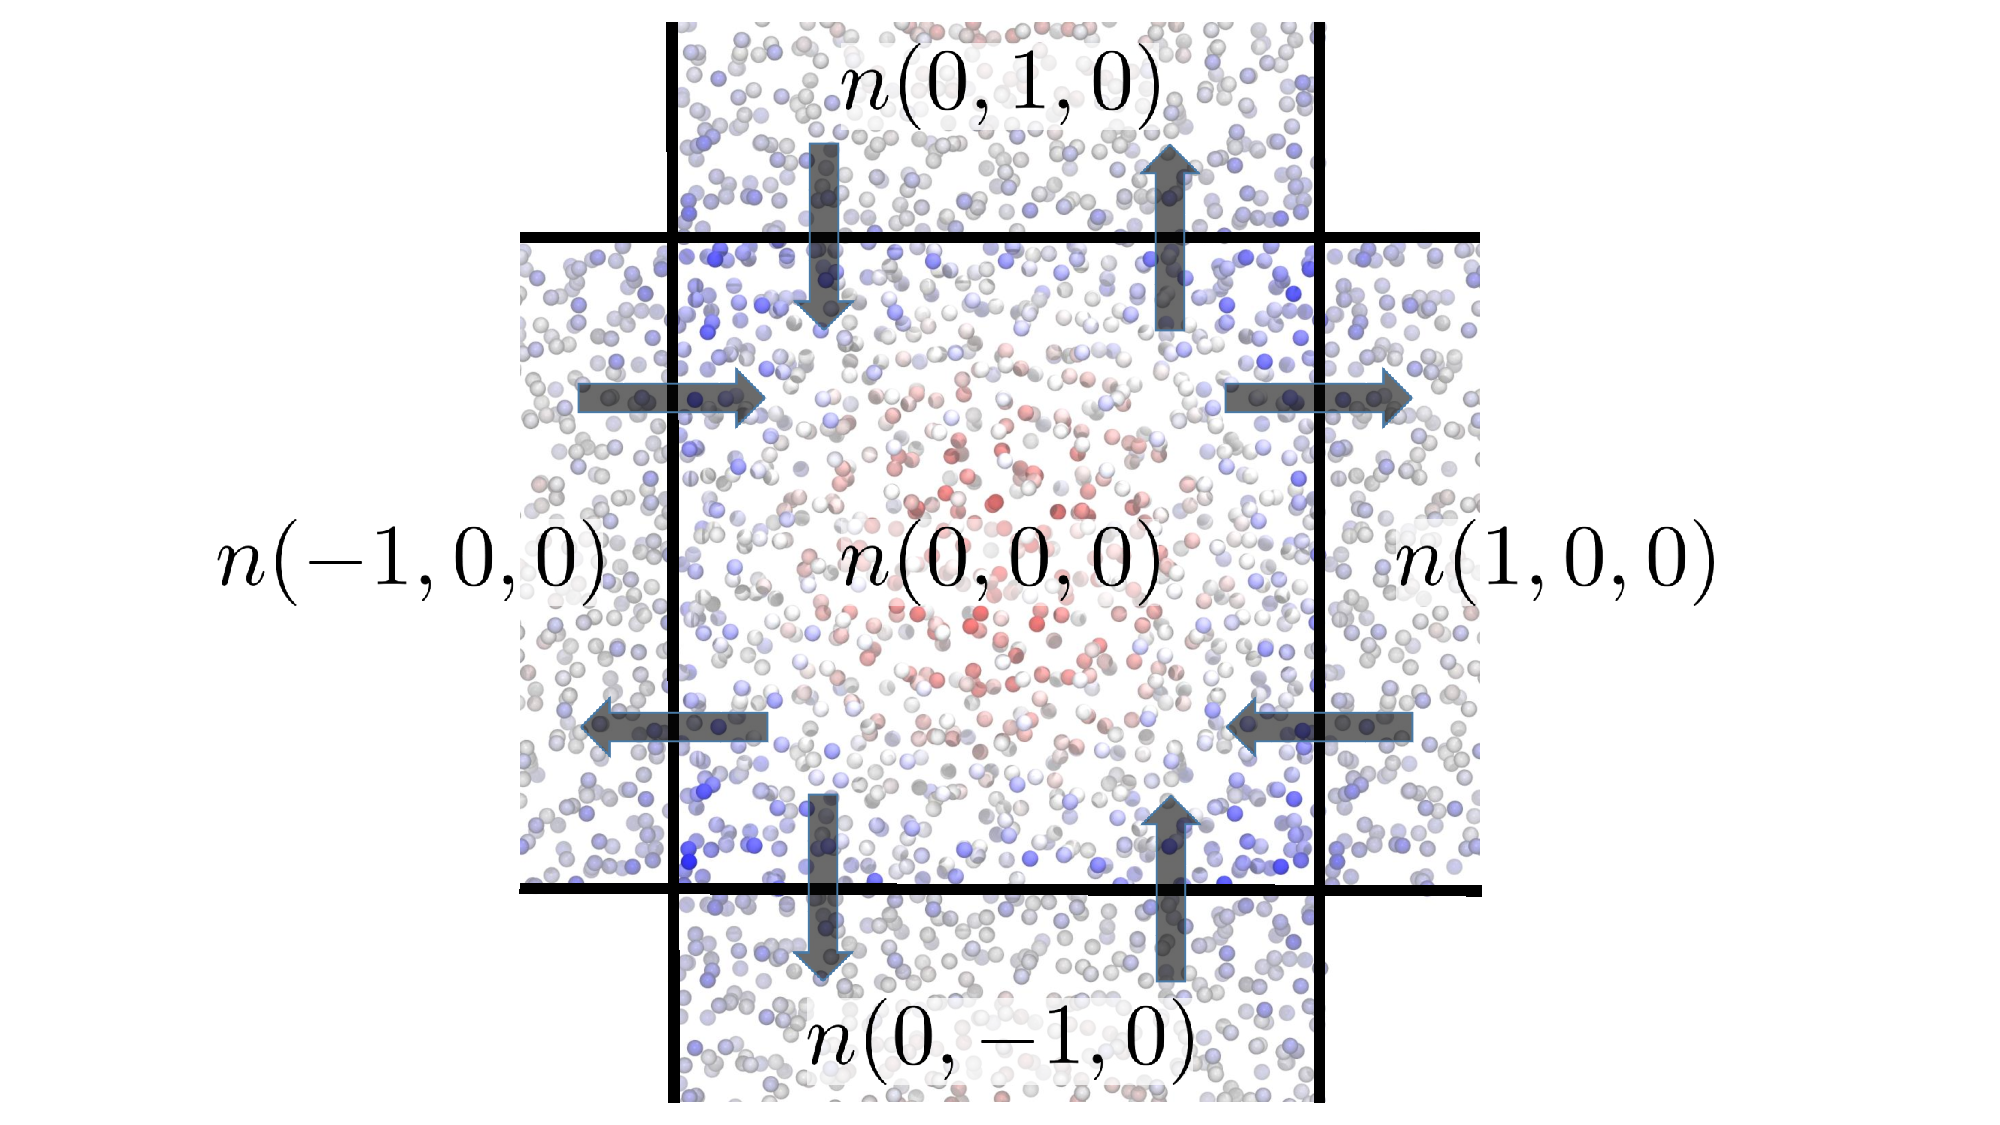
\includegraphics[width=0.98\linewidth]{images/pbc_example.pdf}
      \caption[Cartoon of a cubic periodic system]{Cartoon of a periodic cell with cubic lattice vectors of 
      length, \emph{L}. Particles are colored on a spectrum from red $\rightarrow$ white $\rightarrow$ blue
      by distance from the center of the cell. Each arrow is coupled with the one opposite it and indicates
      the direction of particle exchange between the unit cell \emph{n}(0,0,0) and the image cells 
      \emph{n}($\pm$x,$\pm$x,0). Because the motions are coupled between the unit and image cells, a particle
      exiting \emph{n}(0,0,0) and crossing into \emph{n}(1,0,0) is mirrored in \emph{n}(-1,0,0) as crossing 
      into \emph{n}(0,0,0) on the other side of the box.}
      \label{fig:pbc}
  \end{figure}
  
  \subsection{\label{ch2:sec3:level4}The Ewald summation}
  Assume we have a distribution of both positive and negative point charges scattered about a periodic and cubic
  cell of length, \emph{L}, and volume, \emph{L}$^{3}$. The total number of particles is \emph{N} and while we
  generally want \emph{N}/2 positive and \emph{N}/2 negative charges for charge neutrality, the discussion here
  will make no such demands. This makes sense especially since we are simulating \emph{infinitely dilute} single 
  ions where the unit cell is expected to take the same net charge as the ion inside. We want to calculate the
  Coulomb contribution to the potential energy of the system, which is expressed using a direct summation in Eq.
  \ref{directsum} (as in above sections, Gaussian units are assumed).
  
  \begin{equation}\label{directsum}
      U_{Coulomb} = \frac{1}{2} \sum_{i=1}^{N} \sum_{j=1}^{N} \sideset{}{'}\sum_{\textbf{n} \in \mathbb{R}} 
      \frac{q_{i}q_{j}}{\left|r_{ij} + \textbf{n}L\right|}
  \end{equation}
  
  The double sum runs over particle indices \emph{i} and \emph{j} up to the total number of particles \emph{N}
  over all cubic lattices where \textbf{n} = ($n_{x}$, $n_{y}$, $n_{z}$). $n_{x}$, $n_{y}$, and $n_{z}$ are
  integers which provide for the location of the lattice in 3D space, $\mathbb{R}$. The prime indicates that the 
  \textbf{n} = 0 sums should omit the \emph{i} = \emph{j} case so a particle does not interact with itself. In 
  principle the infinite sum of the series gives the true Coulomb energy in a lattice -- keyword, \emph{infinite}.
  To solve numerically, a finite set of lattice vectors are used under the assumption that as the distance from 
  the unit cell increases, the contribution to the potential will decrease as well. However, because the sum 
  converges very slowly a large cutoff must still be used to achieve sufficient accuracy. Combine this with a 
  hefty computational overhead of \textbf{\emph{O}}(\emph{N}$^{2}$) on the direct sum and it's easy to see why 
  a more efficient solver is desired. Ideally, an algorithm should scale linearly in cost with system size, 
  \textbf{\emph{O}}(\emph{N}). The most widely adopted algorithm in modern MD codes is the Ewald summation 
  \textbf{\emph{O}}(\emph{N}$^{\frac{3}{2}}$) or an even more efficient variant (i.e., particle mesh Ewald
  \textbf{\emph{O}}(\emph{N}log~\emph{N})).
  
  The Ewald summation splits the slowly converging series above into two components which can each be solved
  faster than the direct summation method. The series in 1/\emph{r} is usually split with the use of the error
  function $\erf$($\eta$r) and its complimentary form $\erfc$($\eta$r), where
  
  \begin{equation}
      \frac{1}{r} = \frac{erfc(\eta r)}{r} + \frac{erf(\eta r)}{r}.
  \end{equation}
  
  \noindent $\eta$ is a splitting parameter controlling the length scale and balance between the real space
  part, $\erfc$($\eta$r), and the reciprocal space part, $\erf$($\eta$r). In a cubic unit cell, $\eta$
  has an optimal value of 5.6/\emph{L} measured in \AA~with the real space part truncated to $\sim$10 \AA~and
  the reciprocal space part capturing the rest. The resulting formula takes the form,
  
  \begin{equation}\label{ewald}
   \begin{split}
      U_{Ewald} = &U_{real} + U_{recip} + U_{surf} + U_{self} + U_{net} \\
                = &\frac{1}{2} \sum_{i=1}^{N} \sum_{j=1}^{N} q_{i}q_{j} \left(\sideset{}{'}\sum_{\textbf{n} \in 
                \mathbb{R}} \frac{erfc(\eta\left|r_{ij} + \textbf{n}L\right|)}{\left|r_{ij} + \textbf{n}L\right|} + 
                \sum_{k \in \mathbb{K}, k \neq 0} \frac{4\pi}{L^3}\frac{e^{-\frac{k^2}{4\eta^2}}}{k^2}e^{-ik 
                \cdot r_{ij}}\right) + \\
                  & \frac{2\pi}{\left(2\epsilon^{\prime} + 1\right)L^3} \left(\sum_{i=1}^{N} q_{i}r_{i}\right)^2 + 
                  \frac{\zeta}{2L} \sum_{i}^{N} q_{i}^2 + \frac{\pi}{L^3\eta^2}Q^2,
   \end{split}
  \end{equation}
  
  \noindent where k=$\frac{2\pi}{L}\textbf{n}$ is the reciprocal space lattice vector, $\epsilon^{\prime}$ is the 
  dielectric of the surrounding medium, which is taken as $\infty$ in so-called `tin-foil' or conducting boundary
  conditions common to MD simulations and so vanishes, and Q$^{2}$ is the square of the net charge in the unit cell.
  The self-energy includes a constant $\zeta$ = -2.837297 for a cubic lattice. The corrections beyond the real and
  reciprocal space terms require little to no computational overhead and can sometimes be pre-computed and added in
  as a constant at each timestep, specifically when the volume is constrained. I use the more efficient 
  \textbf{\emph{O}}(\emph{N}$^{\frac{3}{2}}$) scaling algorithm in Chapter \ref{ch6:sec1:level1} for generating 
  trajectories but use a single sum version of the formula as presented in Eq. \ref{ewald} to compute the local 
  potential I described in Chapter \ref{ch1:sec4:level1}.
  
  \subsection{\label{ch2:sec3:level5}Equations of motion and time propagation}
  Once we have evaluated the potential energy of a configuration of particles, we calculate the force as the negative
  derivative of the potential with respect to the coordinate, $-\frac{\partial U}{\partial r}$. With forces in hand,
  we have a variety of mathematics to choose from to update the particle positions. One of the simplest and most 
  effective integrators is called the Verlet algorithm which is nearly universally available in modern MD codes.
  This method results from a Taylor series expansion in \emph{r} about time, \emph{t},
  
  \begin{equation}
      r(t+\delta t) \approx 2r(t) - r(t-\delta t) + \frac{f(t)}{m}\delta t^2,
  \end{equation}
  
  \noindent where $\delta$t is the length of the timestep and $\frac{f(t)}{m}$ is the acceleration on the particle
  for the current configuration. To compute the new location of a particle, various algorithms will require knowledge
  of one or more previous locations. The velocity of the particle can be computed from
  
  \begin{equation}
      v(t) = \frac{r(t+\delta t) - r(t-\delta T)}{2\delta t},
  \end{equation}

  \noindent which is accurate to order $\delta t^{2}$. From this, the kinetic energy and the system temperature can 
  be constructed. We'll see in the next section that this relation is important in monitoring the stability of a 
  simulation and/or conditioned so as to compare to an experiment under the same conditions.

  \subsection{\label{ch2:sec3:level6}Thermodynamic ensembles: controlling the variables}
  Thermodynamic ensembles are relations which establish a complete statistical knowledge of a system under certain
  conditions that are linked to macroscopic observables such as particle number, \emph{N}, temperature, \emph{T},
  energy, \emph{U}, or volume, \emph{V}. The natural ensemble for molecular dynamics simulations is the 
  \emph{microcanonical ensemble}, S(N,V,U), which is isolated from an external bath and the myriad parts merely 
  exchange the available energy to maximize the entropy throughout. This ensemble, in the limit of large systems,
  approximates the \emph{canonical ensemble} where average temperature is constant. Though in the \emph{canonical ensemble}, 
  this is accomplished through coupling to an external bath. 
  
  In both of these ensembles, the particle number and system volume are also fixed. The bath allows endo-/exothermic 
  processes to absorb/release excess energy through artificial modification of particle velocities. The \emph{canonical 
  ensemble} is widely used in molecular dynamics as precise control of the temperature is often necessary for studies of 
  protein folding, solvation thermodynamics, transport properties, etc. 
  
  The third most commonly used ensemble in molecular  dynamics is the \emph{isobaric-isothermal ensemble} where particle 
  number and temperature remain fixed as in the \emph{canonical ensemble} but the volume of the system is allowed to change
  to match a desired pressure. Motivations for controlling the pressure are similar to those for precise control on the 
  system temperature. Simulations incorporate barostats which scale the unit cell size in response to the virial pressure
  tensor which depends on the forces on the atoms. This ensemble is commonly used to relieve strain on the solvent after 
  adding large solutes such as proteins or other biomolecules to the unit cell and achieve a proper solvent density 
  especially at the cell edges. 
  
  Molecular dynamics relies on the ergodic principle to generate statistical averages of the behavior of molecular 
  systems through equivalence of averages in time to ensemble averages over all space. We must take great care with the 
  selection of an algorithm to constrain a particular property that it does not violate this condition, such as the original 
  Nos$\acute{e}$-Hoover thermostat. In the limit of large system size (\emph{N} $\rightarrow \infty$) the averages in 
  properties measured from each of the ensembles become identical. And so for the free energy work below, there is often
  very little difference between the averages computed in the (NVT) or (NpT) thermodynamic ensembles\cite{tlbbook}.
  
 \section{\label{ch2:sec4:level1}Free energy calculations using molecular dynamics}
 A knowledge of free energy and temperature derivatives is essential in advancing our understanding of a number of physical 
 phenomena including binding and equilibrium constants, rate constants of reactions, pH, pKa, activity coefficients 
 (solubilities), osmotic coefficients, surface tension, and partitioning behavior between phases (including phase transitions). 
 I will first present common methods for directly calculating free energies from molecular dynamics simulations. This will
 be followed by a thorough derivation and discussion of the quasichemical theory used in later chapters. The quasichemical 
 method partitions the solvation free energy through spatial conditioning. Taken together, the fragments add to the conventional
 solvation free energy but offer additional information not available to the other methods discussed here. The quasichemical 
 theory is particularly well-suited for the determination of single-ion solvation free energies because it is able to uniquely
 separate the local and distant solvation effects.
 
 The format of equations and general outline are modeled after Refs. \cite{smit,tlbbook}. The wording is otherwise original.
 
 \subsection{\label{ch2:sec4:level2}Free energy perturbation and thermodynamic integration}
 Free energy perturbation is one of the oldest and most successful methods for computing free energy differences between a
 reference state (A) and a target state (B). Recall that in the canonical ensemble, the Helmholtz free energy has the form,
 
 \begin{equation}\label{helmholtz}
     F(N,V,T) = -\frac{1}{\beta}\ln~Q_{NVT}.
 \end{equation}
 
 \noindent $\beta$ is the inverse temperature $\frac{1}{k_{B}T}$ and Q$_{NVT}$ is the canonical partition function. The partition 
 function can be split into coordinate and momentum space contributions, leading to an excess and an ideal contribution, 
 respectively.
 
 \begin{equation}\label{q_nvt}
  \begin{split}
      Q_{NVT} &= \frac{1}{N!}\frac{1}{h^{3N}}\int dp e^{-\beta\mathcal{K}} \int dq e^{-\beta\mathcal{V}} \\
              &= Q^{id}_{NVT}Q^{ex}_{NVT}
  \end{split}
 \end{equation}
 
 \noindent The ideal part is an analytical expression,
 
 \begin{equation}\label{q_id}
     Q^{id}_{NVT} = \frac{V^N}{N!\Lambda^{3N}}
 \end{equation}
 
 \noindent where the thermal de Broglie wavelength is $\Lambda = \sqrt{h^2/2\pi mk_{B}T}$. The excess part is
 
 \begin{equation}\label{q_ex}
     Q^{ex}_{NVT} = V^{-N}\int dr e^{-\beta\mathcal{V}(r)}.
 \end{equation}
 
 The free energy difference in the canonical ensemble, is
 
 \begin{equation}\label{fep}
     \Delta F(A\rightarrow B) = -\frac{1}{\beta}\ln\left<e^{-\beta\left(\mathcal{V}_{B}-\mathcal{V}_{A}\right)}\right>_{A}.
 \end{equation}
 
 \noindent $\mathcal{V}_{A}$ is the potential energy of the system in its reference state, and $\mathcal{V}_{B}$ is the energy
 of the system in the target state. The subscript indicates configurations are generated in the reference state. Angled brackets 
 indicate ensemble averaging. The single-perturbation result is only considered accurate if states A and B are very similar with
 strong overlap between the energy landscape outlined by their respective partition functions. If the mass does not change with 
 the perturbation, the ideal part vanishes. 
 
 Free energies between states with large perturbations (i.e., opposite charges, structural isomers, etc.) can be modeled as 
 incremental changes in the chemical properties of A to match B -- also known as `alchemical transformation.' The intermediate 
 states can be entirely fictitious so long as the i\emph{th} and (i+1)\emph{th} states are sufficiently similar. A coupling 
 parameter $\lambda$ is used to smoothly vary the A-state to B over (N-1) intervals. The coupling parameter can be chosen to 
 alter a single property at a time or several.
 
  \begin{equation}\label{alchemical}
     \Delta F(A\rightarrow B) = -\frac{1}{\beta} \sum_{i=1}^{N-1} \ln\left<e^{-\beta\left(\mathcal{V}_{\lambda_{i+1}}-\mathcal{V}_{\lambda_{i}}\right)}\right>_{\lambda_{i}}
 \end{equation}
 
 An alternative approach that also sees a great deal of use in the community is the thermodynamic integration method. This is 
 similar to the alchemical transformation approach described above in that we are attempting to connect two chemically 
 dissimilar endpoints using fictitious intermediates. However, instead of sampling the ensemble average in the difference of
 the energies between the (i+1)\emph{th} and i\emph{th} states, we sample the ensemble average of the derivative of the 
 potential with respect to the coupling parameter and then integrate,
 
 \begin{equation}\label{ti}
     \Delta F(A\rightarrow B) = \int_{0}^{1} d\lambda \left< \frac{\partial \mathcal{V}(\lambda)}{\partial \lambda}\right>_{\lambda}.
 \end{equation}
 
 As with free energy perturbation, numerous independent simulations at each $\lambda$ are required to assemble the final result. 
 These paths can be used to compute relative ion solvation free energies (e.g., K$^{+}$ to Na$^{+}$ or K$^{+}$ to Cl$^{-}$) and 
 absolute ion solvation free energies where the reference state is the ion uncoupled from the solvent. The ideal part of the free 
 energy is dropped here because it can be determined analytically, while the excess part is both the more interesting part and 
 far more difficult to compute. It is desirable to devise methods which require very few calculations for this excess part.
 
 \subsection{\label{ch2:sec4:level3}The potential distribution theorem}
 The potential distribution theorem of Widom \emph{sometimes called the particle insertion method} was developed to compute the 
 \emph{excess} chemical potential (i.e., partial molar free energy) of a solute in pure liquids or complex mixtures. In the 
 canonical ensemble, the excess chemical potential of a distinguished ion ($\alpha$) is
 
 \begin{equation}\label{mu}
     \mu^{ex}_{\alpha} = -\frac{1}{\beta}\ln\left<e^{-\beta\Delta\mathcal{V}}\right>_{0}; \quad\quad \textrm{where,} \quad \Delta\mathcal{V} = \mathcal{V}(N+\alpha)-\mathcal{V}(N)-\mathcal{V}(\alpha).
 \end{equation}
 
 \noindent $\Delta\mathcal{V}$ is the interaction energy between the ion and the solvent, with an ensemble average computed over
 configurations sampled with the ion uncoupled from the solvent (as indicated by the subscript `0'). The quantity is more 
 often expressed as
 
 \begin{equation}\label{bmu}
     \beta\mu^{ex}_{\alpha} = -\ln\left<e^{-\beta\Delta\mathcal{V}}\right>_{0}
 \end{equation}

 \noindent with an inverse form

 \begin{equation}\label{invbmu}
     \beta\mu^{ex}_{\alpha} = \ln\left<e^{\beta\Delta\mathcal{V}}\right>
 \end{equation} 
 
 \noindent where the sampling is now done over configurations which include the fully coupled ion/solvent interactions.
 Rearranging Eq. \ref{bmu} gives
 
 \begin{equation}\label{pmu}
     e^{-\beta\mu^{ex}_{\alpha}} = \left<e^{-\beta\Delta\mathcal{V}}\right>_{0} = \int d\varepsilon P_{\alpha}^{(0)}(\varepsilon)e^{-\beta\varepsilon}
 \end{equation}

 \noindent where $P_{\alpha}^{(0)}(\varepsilon) = \left<\delta\left(\varepsilon-\Delta\mathcal{V}\right)\right>_{0}$ is 
 a probability distribution of ion/solvent interaction energies from an uncoupled trajectory. Conversely, the distribution 
 from the fully coupled trajectory is $P_{\alpha}(\varepsilon) = 
 \left<\delta\left(\varepsilon-\Delta\mathcal{V}\right)\right>$. Using the law of averages we can relate these two 
 distributions through
 
 \begin{equation}\label{cross}
     P_{\alpha}(\varepsilon) = e^{-\beta\left(\varepsilon-\mu^{ex}_{\alpha}\right)}P_{\alpha}^{(0)}(\varepsilon).
 \end{equation}
 
 \noindent The crossing point of these distributions at some interaction energy $\varepsilon$ will yield the exact excess 
 chemical potential. If however, the distributions do not overlap, the method fails outright. The excess chemical potential
 can be assessed from one of the distributions as well, though the wings of these distributions are poorly, if ever, sampled
 over the course of a simulation making it difficult to integrate accurately. The quasichemical theory I discuss next addresses
 this by applying spatial conditioning to the interaction energy distributions. This removes the need to sample rare events 
 at the high- and low-energy tails of the distributions and yields Gaussian or nearly-Gaussian behavior in 
 $P_{\alpha}(\varepsilon)$. The conditioning is done using hard spheres with interaction energies computed only when all solvent
 is beyond a certain distance, or by adding an external potential into the simulation to push the solvent away. The latter is
 done gradually using thermodynamic integration.

 \subsection{\label{ch2:sec4:level4}Quasichemical theory}
 This section borrows equation format and outline from Refs. \cite{shi2013length,tlbbook}. The wording is otherwise
 original.
 
  \subsubsection{\label{ch2:sec4:level4:zone1}Hard sphere conditioning}
  Recall that the excess chemical potential of a monoatomic ion may be evaluated using the following expressions, derived 
  from the potential distribution theorem,

  \begin{equation}
   \begin{split}
    \beta\mu\sur{ex} &= -\mathrm{ln}\left<e^{-\beta\Delta\mathcal{V}}\right>\sous{0} \\
                     &=  \mathrm{ln}\left<e^{\beta\Delta\mathcal{V}}\right>,
    \label{eqn:pdt}
   \end{split}
  \end{equation}

  \noindent where $\beta = 1/k\sous{B}\mathrm{T}$ and $\Delta\mathcal{V}$ is the interaction energy between ion
  and solvent. Brackets indicate ensemble averaging. The subscript zero implies uncoupled ion/solvent motions
  during sampling and fully coupled ion/solvent interactions in the second case. In both cases, full 
  solvent/solvent interactions are in place. Inclusion of a hard-sphere cavity potential with radius, \emph{r}, 
  in the above expressions allows us to spatially separate contributions to the free energy,

  \begin{equation}
   \begin{split}
    \beta\mu\sur{ex} &= \mathrm{ln}\left<e^{-\beta\mathcal{V}\sous{HS}(r)}\right> - \mathrm{ln}\left<e^{-\beta\mathcal{V}\sous{HS}(r)}\right>\sous{0} - 
                        \mathrm{ln}\left<e^{-\beta\Delta\mathcal{V}}\right>\sous{\mathcal{V}\sous{HS}(r)} \\
                     &= \mathrm{ln}x\sous{0}(r) - \mathrm{ln}p\sous{0}(r) - \mathrm{ln}\left<e^{-\beta\Delta\mathcal{V}}\right>\sous{\mathcal{V}\sous{HS}(r)} \\
                     &= \mu\sursous{ex}{is}(r) + \mu\sursous{ex}{pk}(r) + \mu\sursous{ex}{os}(r).
    \label{eqn:hsqct}
   \end{split}
  \end{equation}

  Above, \emph{x}\sous{0} is the inner shell (is) term which is the probability of finding no solvent in the 
  excluded volume defined by $\mathcal{V}$\sous{HS} with full ion/solvent interactions, \emph{p}\sous{0} is 
  the packing (pk) term which is the probability of finding no solvent in this same cavity placed in pure 
  solvent, and the final term is the outer shell (os) or long-range term corresponding to the residual 
  interaction energy of the ion with solvent molecules beyond this excluded volume. A hard-sphere potential 
  suffices for small cavities typically around 0.3 nm or less, beyond which \emph{x}\sous{0} and 
  \emph{p}\sous{0} are generally poorly sampled in typical simulations. An external potential applied to the
  solvent is critical for reaching length scales far enough to see convergence in the interfacial potentials
  monitored as the mean-field electrostatic potential at the cavity's core.
  
  \subsubsection{\label{ch2:sec4:level4:zone2}Soft-core conditioning}
  I can reach any length scale by gradually introducing a soft-core M(\emph{r})-potential instead (Eq. \ref{eqn:scqct}).
  
  \begin{equation}
   \begin{aligned}
    \beta\mu\sur{ex} &= \mathrm{ln}\left<e^{-\beta M(r)}\right> - \mathrm{ln}\left<e^{-\beta M(r)}\right>\sous{0} - 
                        \mathrm{ln}\left<e^{-\beta\Delta\mathcal{V}}\right>\sous{M(r)} \\
                     &= \mathrm{ln}\left<e^{-\beta M(r)}\right> - \mathrm{ln}\left<e^{-\beta M(r)}\right>\sous{0} +
                        \mathrm{ln}\left<e^{\beta\Delta\mathcal{V}}\right>_{M(r)+\Delta\mathcal{V}}
    \label{eqn:scqct}
   \end{aligned}
  \end{equation}  
  
  In this framework, the packing and inner shell parts of the solvation free energy are captured by the work to dig
  a cavity in the bare solvent and around the ion, respectively. The inner shell portion is often referred to as the
  chemical part of the free energy as it's magnitude reflects the intensity of the interactions between the ion with 
  the retreating solvent. The thermodynamic integration procedure and M(\emph{r})-potential used in Chapter 
  \ref{ch6:sec1:level1} are the same as in a previous study\cite{shi2013length}. This arrangement requires two simulations
  for the outer shell contribution where ion/solvent interaction energy distributions are sampled from an uncoupled 
  and a separate coupled trajectory. The cavity radius, \emph{r}, should be tuned such that both distributions are
  accurately Gaussian. A mean-field approximation to $\mu$\sursous{ex}{os} can be obtained this 
  way\cite{hummer1996, hummer1998}, but as Shi and Beck demonstrated especially for anions, the fluctuation terms often
  do not match until reaching extreme length scales which can lead to inaccuracies\cite{shi2013length}. This behavior 
  has quite a bit to do with the similarities in the solvation shell between a neutral particle and one bearing 
  $\pm$q charge (e.g., orientation of solvent dipoles). I discuss more on this later in Chapter \ref{ch6:sec1:level1}.

  To work around this issue I invoke the midpoint-rule to generate an approximation to the long-range term from a 
  single simulation. Here the average interaction energy is sampled from a half-coupled trajectory where the ion's 
  charge is halved but all other interactions are unchanged. The approximation is accurate to second order in 
  perturbation theory and has proven remarkably reliable in previous free energy work\cite{beck2011lmft, shi2013length}.

\end{theory}
 % theory
 \begin{sie}
 \chapter{Toward a quantitative theory of Hofmeister effects: from quantum effects to thermodynamics}
 \hyperlink{toc}{Return to TOC}
  \section{\label{ch3:sec0:level1}Preface}
  This chapter draws text and data from a published article,
  
  \vspace{12pt}
  \noindent \emph{Travis P.~Pollard, Thomas L.~Beck, Toward a quantitative theory of Hofmeister phenomena: From quantum effects to 
  thermodynamics, Current Opinion in Colloid $\&$ Interface Science, Volume 23, June 2016, Pages 110-118.}
  \vspace{12pt}
  
  \noindent Additional data is supplied here that will be published in a forthcoming article. 
  
  These articles concern the local solvation structure around the alkali/halide ions which is critical in developing a quantitative 
  theory of the specific ion effects discussed throughout Chapter \ref{ch1:sec1:level1}. This is because the solvation structure is
  shaped not only by electrostatic forces but also dispersion and induction contributions, which requires electronic resolution. Recent 
  simulation work has also observed that charge transfer between anions to surrounding waters decreases overall solvation asymmetry. 
  I sought to explore the relationship between solvation structure and the presence of these non-electrostatic forces. To do this, I 
  carried out a series of electronic structure calculations to optimize myriad X$^{\pm}$(H$_{2}$O)$_{n}$ clusters, where X is one of 
  Li$^{+}$, Na$^{+}$, K$^{+}$, F$^{-}$, Cl$^{-}$, or Br$^{-}$, and \emph{n} = 1, \dots, 6. Following this, I used the symmetry adapted 
  perturbation theory (discussed in Chapter \ref{ch2:sec2:level1}) to extract interaction energies and components. Energies are complemented
  with the use of quantum theory of atoms in molecules to estimate the ion charge from gas phase to several states with a (nearly) 
  completed first solvation shell. From this I learned that dispersion and induction forces make up approximately $\frac{1}{3}$ of
  the attractive contributions to the interaction energy for anion/water clusters -- though, these effects tended to (nearly) saturate
  within the first shell regardless of ion charge. I also discovered that the symmetry adapted perturbation theory is not suitable to 
  estimating the stabilization energy of ion/water complexes due to partial charge transfer. However, I proposed that it may be better 
  suited to providing an upper bound on the polarization energy. Combined with the polarized orthogonally localized molecular orbital
  method, the polarization energy can be bounded from below too (this likewise produces upper and lower bounds to the charge transfer 
  energy). However, assuming the relative values for a given ion and cluster size were qualitatively correct, I found that for 
  F$^{-}$(H$_{2}$O)$_{6}$, the charge transfer interaction energy favored clusters where the ion was internally solvated (as opposed
  to surface solvated). This is consistent with the findings of others which suggest that the inclusion of partial charge transfer 
  in simulation promotes the reduction of solvent distribution anisotropy around the ion.
  
  This section addresses three of the questions I posed in Chapter \ref{ch1:sec1:level4},

  \begin{itemize}
      \item What sort of interactions? 
      \item How strong are they relative to one another?
      \item Do we need electronic structure theory to solve everything?
      \item Will a simpler model work far away from the ion?
  \end{itemize}
  
  \section{\label{ch3:sec1:level1}Computational methods}
  This chapter covers the findings outlined in two separate studies. In this case, the studies share a significant degree of overlap so a 
  combined methods section is covered below.
  
   \subsection{\label{ch3:sec1:level2}Optimization and atomic partial charges}
    Small ion/water clusters were optimized to the SCS-MP2/CVTZ level of theory\cite{grimme2003scsmp2} (details of the basis sets used are 
    explained later) using the Orca 3.0.3 quantum chemistry package\cite{neese2012orca,valeev2014libint}. A number of favorable initial 
    geometries were extracted from the literature for each cluster size to explore the variation in charge transfer that accompanies partial 
    solvation\cite{kim1999bigf,kim2000smallall,kim2002bigall}. Molden-type inputs of the MP2 natural orbitals were converted 
    to standard wave function files (WFN) using the molden2aim script available here, (\url{http://people.smu.edu/wzou/program/}). The electron 
    density was partitioned by computing the so-called zero-flux surface about the ion within the framework of the quantum theory of atoms 
    in molecules (AIM) pioneered by Bader\cite{bader1990book}. Calculations were carried out for each of the complexes and also the isolated 
    fragments with the difference in the net charge values taken as an estimate of the charge exchanged upon complexation. AIM calculations 
    were performed using the AIMAll package\cite{bader1982proaim,keith2012aimall}. All data necessary for visualization of electron 
    density surfaces or contours were generated using Multiwfn\cite{lu2012multiwfn} and viewed using VMD\cite{humphrey1996vmd} (surface) or the 
    native plotting utility in Multiwfn (contours).

   \subsection{\label{ch3:sec1:level3}Energy decomposition using symmetry adapted perturbation theory}
    Interaction energies were computed at the density fit SCS-MP2 level of theory with counterpoise corrections\cite{boys1970bsse} and the 
    SAPT2+3(CCD)\cite{jeziorski1994sapt,hohenstein2010df,hohenstein2012sapt} level of theory using the open source Psi4\cite{sherrill2012psi4} 
    software. We report the error in the exchange-induction coupled terms at 2\sur{nd}- and 3\sur{rd}-orders of SAPT but otherwise do not scale the
    affected terms as discussed elsewhere in the literature\cite{hohenstein2011scale,herbert2012break}. Errors in the SAPT energies relative
    to SCS-MP2 are in the neighborhood of 6-8\% for the largest cluster sizes with SAPT almost always overshooting the counterpoise-corrected 
    estimate.
    
   \subsection{\label{sec3:sec1:level4}The charge transfer energy}
    The Hellmann-Feynman theorem states that once an electron distribution has been solved, all forces within the system can be calculated
    purely through classical electrostatics and the Coulomb operator. Partitioning of these energies has a physical basis but is purely
    `modeling' in many cases\cite{politzer2015mathematical}. However, this modeling is imported into classical force fields which tends to 
    make them more accurate and so it is instructive to partition energies into separable components in an attempt to translate them to simpler
    force field based simulation. As an interesting aside, non-variational methods (e.g., MP2) do not satisfy the Hellmann-Feynman theorem\cite{jensen2013introduction}.
    Nevertheless, charge transfer contributions to the interaction energy between ion/water clusters were modeled using a pair of partitioning schemes
    within the symmetry adapted perturbation theory (SAPT)\cite{jeziorski1994sapt}. We'll refer to these methods as SM09 and reg-SAPT. The
    SM09 method was outlined by Stone et al. and entails taking the difference in the induction energy to arbitrary order between a dimer-
    centered and monomer-centered basis set calculation\cite{stone2009ct}. In this case, charge transfer is modeled only as a basis set 
    superposition error artifact and so vanishes in the limit of a complete basis. Recent work by Lande et al. has shown this method to be 
    most `reliable' for moderate-sized basis sets, e.g., aug-cc-pVTZ\cite{lande2015cdftct}. To overcome the shortcomings of the SM09 method,
    Misquitta replaced the monomer-centered basis calculation with one in which the nuclear potential of each fragment is screened from the
    opposite\cite{misquitta2013regsapt}. Inclusion of the screening potential prevents charge transfer but allows for polarization. The sole 
    adjustable parameter in the method is the length scale of the screening potential which is modeled as a Gaussian \emph{s}-orbital with
    width, $\eta$. Misquitta found that $\eta =$ 3.0 au (units are L\sur{-2}) was sufficient for most applications involving the first and 
    second row elements\cite{misquitta2013regsapt}. The parameter is tuned by minimizing the difference in the total induction energy,
    E\sursous{(2)}{ind,tot}, between the dimer- and monomer-centered basis over a range of intermolecular separations, including some points
    below the equilibrium bond length. Tuning was only done for ion/water dimers. Anions presented a bit of a challenge in that the differences
    varied little with changes in the width of the screening orbital. We selected the value in the range of $\eta =$ 1.0 au to 3.0 au which
    also minimized the change in E\sursous{(2)}{ind,tot} computed with the dimer-centered basis set alone. Once a range parameter is determined,
    the charge transfer energy is simply equal to the difference in induction energies computed with and then without the conditioning, both
    using a dimer-centered (or extended monomer-centered) basis representation. These energies exhibit significantly less variance with 
    increasing basis set size. SM09 calculations were performed up to the SAPT2 level using the cc-pVTZ (+ diffuse, where appropriate and 
    def2-TZVPP for K\sur{+})\cite{dunning1989h,dunning1992of,dunning1993cl,dunning1999br,hattig2002ri,rappoport2010def2,rappoport2015kri}
    with the Psi4 package\cite{sherrill2012psi4,hohenstein2010df,hohenstein2012sapt}. Regularized SAPT was handled with the regSAPT
    script included in the SAPT2008 package\cite{jeziorski2012sapt}. The rather dated ATMOL1024 SCF interface\cite{saundersatmol} to the SAPT2008 
    package required an additional change in basis set due to small contraction and total orbital limits. All clusters were successfully modeled with 
    (aug-)cc-pVDZ (Feller's CVDZ) and the (aug-)pc-1 polarization consistent basis 
    set\cite{jensen2001principles,jensen2002diffusefxns,jensen2004cl,jensen2007lina,jensen2012kbr}. However we 
    addressed optimization of the regularization length scale with the def2-QZVPP (+ diffuse, where appropriate) basis\cite{rappoport2010def2}
    and these results are listed in Table \ref{tab:ion_params}. All basis sets were retrieved from the EMSL Basis Set Exchange\cite{emsl1996,emsl2007}.
    
\begin{table}
 \begin{center}
  \begin{tabular}{lc}
   \hline
   \hline
    A & $\eta$ \tabularnewline
   \hline
    H         & 3.0  \tabularnewline
    Li\sur{+} & 3.0  \tabularnewline
    O         & 3.0  \tabularnewline
    F\sur{-}  & 2.5  \tabularnewline
    Na\sur{+} & 3.0  \tabularnewline
    Cl\sur{-} & 1.5  \tabularnewline
    K\sur{+}  & 1.5  \tabularnewline  
    Br\sur{-} & 1.5  \tabularnewline 
   \hline 
   \hline
  \end{tabular}
 \end{center}
 \caption[Optimal range parameters for regularizing potential]{\label{tab:ion_params} Optimal $\eta$ parameters for each element in atomic units ($\eta$ 
 has units of L\sur{-2}). These results support the conclusion of Misquitta that an $\eta$ value near 3.0 au produces adequate screening for the first and 
 second row elements.}
 \end{table}

   \subsection{\label{ch3:sec1:level5}Basis sets}
    Geometry optimization and subsequent generation of WFN files for use with the AIMAll package was carried out with a triple-$\zeta$ quality 
    basis with core-valence functions included for second row and beyond elements 
    (aug-cc-pwCVTZ)\cite{dunning1989h,peterson2002ofcl,peterson2007br,peterson2011lina}. Diffuse functions were removed from the 
    cation basis sets to be consistent with K\sur{+} which had to be modeled with Feller's CVTZ\cite{feller1995k} due to a lack of parameterization 
    in the Dunning sets. The emphasis on density fitting algorithms in Psi4 ultimately required us to pursue the valence-only flavors of the preceding
    basis sets (we substituted the def2-TZVPP basis in for K\sur{+} calculations\cite{rappoport2010def2,rappoport2015kri}). For density fit procedures 
    a Cholesky decomposed basis was constructed with a tolerance 1e-4.
    
  \section{\label{ch3:sec2:level1}Results $\&$ Discussion}
  \subsection{\label{ch3:sec2:level1:chasm1}Interaction energies, atoms in molecules, and partial charges}
  I begin with a survey of the SAPT2+3 (CCD) interaction energies for clusters with up to 6 attached waters, see  Tables \ref{tab:sapt1}--\ref{tab:sapt4}. 
  Even a cursory look over these data confirms the presence of a great deal of ion specificity across all of the components of the interaction energies 
  -- especially in the induction and dispersion contributions for F\sur{-} clusters relative to both Cl\sur{-} and Br\sur{-}.

\begin{table}
 \begin{center}
 \begin{tabular}{lrrrrccrr}
   Cluster & Elst & Ind & Disp & Exch & Exch Err & E\sur{PT} & E\sur{CP} \tabularnewline
  \hline
  \tabularnewline
   \multicolumn{8}{c}{\textbf{X\sur{\pm}(H\sous{2}O)}}  \tabularnewline
  \tabularnewline
Li\sur{+} C\sous{2v} &-32.90 &-13.52 &-0.68 &12.55 &1.00 &-34.56 &-33.46 \tabularnewline
Na\sur{+} C\sous{2v} &-24.95 & -6.39 &-0.43 & 8.43 &1.00 &-23.33 &-22.53 \tabularnewline
K\sur{+}  C\sous{2v} &-19.73 & -4.78 &-1.73 & 8.73 &1.01 &-17.51 &-16.63 \tabularnewline
F\sur{-}  C\sous{1}  &-44.50 &-29.26 &-7.80 &49.33 &1.03 &-32.23 &-29.35 \tabularnewline
Cl\sur{-} C\sous{1}  &-19.01 & -7.57 &-4.42 &15.41 &1.01 &-15.58 &-14.24 \tabularnewline
Br\sur{-} C\sous{1}  &-16.35 & -6.03 &-4.15 &13.13 &1.01 &-13.39 &-12.18 \tabularnewline
  \tabularnewline
   \multicolumn{8}{c}{\textbf{X\sur{\pm}(H\sous{2}O)\sous{2}}}  \tabularnewline
  \tabularnewline
Li\sur{+} D\sous{2d} &-60.95 &-24.85 & -1.36 &20.85 &1.01 &-66.31 &-63.79 \tabularnewline
Na\sur{+} D\sous{2d} &-47.26 &-12.09 & -0.79 &14.76 &1.00 &-45.38 &-43.76 \tabularnewline
K\sur{+}  D\sous{2d} &-36.63 & -8.05 & -3.10 &14.04 &1.00 &-33.74 &-32.13 \tabularnewline
F\sur{-}  C\sous{2}  &-71.95 &-37.84 &-11.76 &69.29 &1.01 &-52.25 &-48.95 \tabularnewline
Cl\sur{-} C\sous{1}  &-35.03 &-13.09 & -8.02 &26.53 &1.02 &-29.62 &-27.05 \tabularnewline
Br\sur{-} C\sous{1}  &-30.37 &-10.64 & -7.58 &22.82 &1.02 &-25.78 &-23.42 \tabularnewline
  \tabularnewline
   \multicolumn{8}{c}{\textbf{X\sur{\pm}(H\sous{2}O)\sous{3}}}  \tabularnewline
  \tabularnewline
Li\sur{+} D\sous{3}      &-82.63 &-33.99 & -1.82 &24.70 &1.01 &-93.74 &-89.70 \tabularnewline
Li\sur{+} 2+1(C\sous{2}) &-71.65 &-26.84 & -1.42 &21.88 &1.01 &-78.03 &-75.15 \tabularnewline
Na\sur{+} D\sous{3}      &-66.13 &-17.10 & -1.14 &18.88 &1.00 &-65.49 &-62.92 \tabularnewline
Na\sur{+} 2+1(C\sous{2}) &-56.86 &-13.26 & -0.92 &16.08 &1.00 &-54.95 &-52.99 \tabularnewline
K\sur{+}  D\sous{3}      &-52.40 &-11.43 & -4.47 &18.98 &1.00 &-49.32 &-46.89 \tabularnewline
K\sur{+}  2+1(C\sous{2}) &-46.20 &-10.08 & -3.57 &17.07 &1.01 &-42.78 &-40.76 \tabularnewline
F\sur{-}  C\sous{3}      &-89.25 &-40.46 &-14.48 &75.84 &1.00 &-68.46 &-64.43 \tabularnewline
F\sur{-}  2+1(C\sous{s}) &-86.00 &-42.36 &-12.72 &75.89 &1.01 &-65.19 &-61.48 \tabularnewline
Cl\sur{-} C\sous{3}      &-48.54 &-16.14 &-10.92 &33.74 &1.01 &-41.86 &-38.20 \tabularnewline
Cl\sur{-} 2+1(C\sous{s}) &-45.72 &-16.48 & -9.34 &32.49 &1.01 &-39.05 &-36.16 \tabularnewline
Br\sur{-} C\sous{3}      &-42.52 &-13.36 &-10.47 &29.58 &1.02 &-36.77 &-33.33 \tabularnewline
Br\sur{-} 2+1(C\sous{s}) &-40.03 &-13.63 & -8.91 &28.20 &1.01 &-34.37 &-31.69 \tabularnewline
  \hline
 \end{tabular}
 \end{center}
 \caption[Interaction energies for ion/water clusters with \emph{n} = 1, 2, and 3]{\label{tab:sapt1} SAPT2+3(CCD) energy decomposition: 
 electrostatics (Elst), induction (Ind), dispersion (Disp), exchange (Exch), 
 and total interaction energy (E\sur{PT}) in the dimer-centered aug-cc-pVTZ basis set. All energies expressed in kcal/mol. Exch Err is a 
 value quantifying the degree of error in the single-exchange approximation which affects the accuracy of exchange-coupled higher order 
 induction terms. A value greater than unity indicates an overestimation of the induction energy and vice versa. This figure represents
 a large source of error in the difference between E\sur{PT} and the conventional counterpoise-corrected interaction energy, E\sur{CP}.}
\end{table}

\begin{table}
 \begin{center}
 \begin{tabular}{lrrrrccrr}
   Cluster & Elst & Ind & Disp & Exch & Exch Err & E\sur{PT} & E\sur{CP} \tabularnewline
  \hline
  \tabularnewline
   \multicolumn{8}{c}{\textbf{X\sur{\pm}(H\sous{2}O)\sous{4}}}  \tabularnewline
  \tabularnewline
Li\sur{+} S\sous{4}                  & -98.29 &-40.57 & -2.16 &24.38 &1.01 &-116.64 &-111.20 \tabularnewline
Li\sur{+} 3+1(C\sous{2})             & -93.67 &-34.78 & -1.53 &25.39 &1.01 &-104.59 &-101.11 \tabularnewline
Na\sur{+} S\sous{4}                  & -82.16 &-21.50 & -1.60 &21.40 &1.00 & -83.87 &-80.29 \tabularnewline
Na\sur{+} 3+1(C\sous{2})             & -75.69 &-18.12 & -1.23 &19.93 &1.00 & -75.11 &-72.30 \tabularnewline
K\sur{+}  S\sous{4}                  & -66.01 &-14.33 & -5.65 &22.31 &1.00 & -63.70 &-60.47 \tabularnewline
K\sur{+}  3+1(C\sous{2})             & -60.66 &-12.37 & -4.71 &20.16 &1.00 & -57.58 &-54.92 \tabularnewline
F\sur{-}  C\sous{1}                  &-107.86 &-42.49 &-16.68 &83.45 &0.99 & -83.59 &-79.51 \tabularnewline
F\sur{-}  C\sursous{\prime\prime}{1} &-108.26 &-43.64 &-16.84 &85.30 &0.99 & -83.43 &-79.41 \tabularnewline
F\sur{-}  C\sous{4}                  &-102.93 &-42.06 &-16.34 &78.96 &1.00 & -82.37 &-78.06 \tabularnewline
F\sur{-}  3+1(C\sous{s})             &-105.96 &-45.02 &-15.28 &85.82 &1.00 & -80.45 &-76.79 \tabularnewline
Cl\sur{-} C\sursous{\prime}{1}       & -61.65 &-19.84 &-13.70 &41.32 &1.01 & -53.87 &-49.27 \tabularnewline
Cl\sur{-} C\sursous{\prime\prime}{1} & -60.60 &-19.18 &-13.39 &40.60 &1.01 & -52.58 &-48.23 \tabularnewline
Cl\sur{-} C\sous{4}                  & -58.94 &-18.16 &-13.03 &38.07 &1.01 & -52.06 &-47.69 \tabularnewline
Br\sur{-} C\sursous{\prime}{1}       & -54.42 &-16.90 &-13.27 &36.81 &1.02 & -47.79 &-43.38 \tabularnewline
Br\sur{-} C\sursous{\prime\prime}{1} & -53.35 &-16.23 &-12.93 &36.06 &1.01 & -46.45 &-42.30 \tabularnewline
Br\sur{-} C\sous{4}                  & -51.90 &-15.12 &-12.60 &33.78 &1.01 & -45.84 &-41.67 \tabularnewline
  \hline
 \end{tabular}
 \end{center}
 \caption[Interaction energies for ion/water clusters with \emph{n} = 4]{\label{tab:sapt2} SAPT2+3(CCD) energy decomposition: electrostatics 
 (Elst), induction (Ind), dispersion (Disp), exchange (Exch), 
 and total interaction energy (E\sur{PT}) in the dimer-centered aug-cc-pVTZ basis set. All energies expressed in kcal/mol. Exch Err is a 
 value quantifying the degree of error in the single-exchange approximation which affects the accuracy of exchange-coupled higher order 
 induction terms. A value greater than unity indicates an overestimation of the induction energy and vice versa. This figure represents
 a large source of error in the difference between E\sur{PT} and the conventional counterpoise-corrected interaction energy, E\sur{CP}.}
\end{table}

\begin{table}
 \begin{center}
 \begin{tabular}{lrrrrccrr}
   Cluster & Elst & Ind & Disp & Exch & Exch Err & E\sur{PT} & E\sur{CP} \tabularnewline
  \hline
  \tabularnewline
   \multicolumn{8}{c}{\textbf{X\sur{\pm}(H\sous{2}O)\sous{5}}}  \tabularnewline
  \tabularnewline
Li\sur{+} C\sous{2}        &-106.66 &-41.11 & -1.60 &19.44 &1.01 &-129.93 &-124.73 \tabularnewline
Li\sur{+} 4+1(C\sous{2})   &-108.62 &-40.76 & -1.79 &24.97 &1.01 &-126.20 &-121.46 \tabularnewline
Na\sur{+} 4+1(C\sous{2})   & -90.97 &-22.37 & -1.64 &22.05 &1.00 & -92.92 &-89.12 \tabularnewline
Na\sur{+} C\sous{2}        & -84.15 &-24.06 & -1.91 &19.92 &1.00 & -90.20 &-85.82 \tabularnewline
K\sur{+}  4+1(C\sous{2})   & -73.70 &-14.96 & -5.79 &22.77 &1.00 & -71.68 &-68.29 \tabularnewline
K\sur{+}  C\sous{2}        & -58.86 &-15.09 & -5.93 &18.47 &1.00 & -59.40 &-55.81 \tabularnewline
K\sur{+}  4+1(C\sous{1})   & -53.79 &-14.49 & -5.40 &18.92 &1.00 & -54.76 &-51.39 \tabularnewline
F\sur{-}  R3L2             &-119.58 &-43.83 &-18.43 &85.14 &0.99 & -96.70 &-92.03 \tabularnewline
F\sur{-}  R4L              &-118.12 &-43.22 &-18.07 &83.61 &0.99 & -95.80 &-91.37 \tabularnewline
F\sur{-}  L3DL             &-114.53 &-46.02 &-17.39 &86.66 &1.00 & -91.29 &-86.80 \tabularnewline
F\sur{-}  R4A              &-112.76 &-44.37 &-17.10 &83.54 &1.00 & -90.69 &-86.17 \tabularnewline
F\sur{-}  R43f             &-111.75 &-44.42 &-16.99 &83.17 &1.00 & -89.98 &-85.50 \tabularnewline
F\sur{-}  R4L\sur{\prime}  &-112.94 &-44.56 &-17.05 &86.16 &0.99 & -88.39 &-84.17 \tabularnewline
F\sur{-}  R3AA             &-109.36 &-47.27 &-15.78 &86.30 &1.00 & -86.12 &-81.89 \tabularnewline
Cl\sur{-} R4A1             & -67.14 &-22.32 &-14.67 &44.79 &1.01 & -59.34 &-54.53 \tabularnewline
Cl\sur{-} R4A              & -66.57 &-21.19 &-14.36 &43.35 &1.01 & -58.77 &-54.07 \tabularnewline
Cl\sur{-} R43f             & -65.47 &-20.92 &-14.13 &42.65 &1.01 & -57.88 &-53.30 \tabularnewline
Cl\sur{-} R3AA\sur{\prime} & -63.09 &-22.16 &-12.98 &43.02 &1.01 & -55.21 &-51.15 \tabularnewline
Cl\sur{-} R5               & -61.92 &-20.16 &-13.65 &40.66 &1.01 & -55.07 &-50.59 \tabularnewline
Cl\sur{-} R3AA             & -62.01 &-22.20 &-12.86 &42.35 &1.01 & -54.71 &-50.59 \tabularnewline
Cl\sur{-} R4f3             & -62.03 &-22.21 &-12.87 &42.40 &1.01 & -54.71 &-50.58 \tabularnewline
Br\sur{-} R4A1             & -59.22 &-19.09 &-14.29 &40.00 &1.01 & -52.61 &-47.96 \tabularnewline
Br\sur{-} R4A              & -59.07 &-18.20 &-14.06 &39.07 &1.01 & -52.27 &-47.72 \tabularnewline
Br\sur{-} R43f             & -57.89 &-17.84 &-13.78 &38.22 &1.01 & -51.29 &-46.89 \tabularnewline
Br\sur{-} R3AA\sur{\prime} & -55.46 &-18.89 &-12.57 &38.02 &1.01 & -48.90 &-45.03 \tabularnewline
Br\sur{-} R5               & -54.46 &-16.94 &-13.25 &36.16 &1.01 & -48.49 &-44.21 \tabularnewline
Br\sur{-} R4f3             & -54.40 &-18.89 &-12.41 &37.29 &1.02 & -48.41 &-44.89 \tabularnewline
  \hline
 \end{tabular}
 \end{center}
 \caption[Interaction energies for ion/water clusters with \emph{n} = 5]{\label{tab:sapt3} SAPT2+3(CCD) energy decomposition: electrostatics
 (Elst), induction (Ind), dispersion (Disp), exchange (Exch), 
 and total interaction energy (E\sur{PT}) in the dimer-centered aug-cc-pVTZ basis set. All energies expressed in kcal/mol. Exch Err is a 
 value quantifying the degree of error in the single-exchange approximation which affects the accuracy of exchange-coupled higher order 
 induction terms. A value greater than unity indicates an overestimation of the induction energy and vice versa. This figure represents
 a large source of error in the difference between E\sur{PT} and the conventional counterpoise-corrected interaction energy, E\sur{CP}.}
\end{table}

\begin{table}
 \begin{center}
 \begin{tabular}{lrrrrccrr}
   Cluster & Elst & Ind & Disp & Exch & Exch Err & E\sur{PT} & E\sur{CP} \tabularnewline
  \hline
  \tabularnewline
   \multicolumn{8}{c}{\textbf{X\sur{\pm}(H\sous{2}O)\sous{6}}}  \tabularnewline
  \tabularnewline
Li\sur{+} D\sous{2d}      &-118.06 &-42.73 & -2.22 &24.80 &1.01 &-138.22 &-132.30 \tabularnewline
Li\sur{+} 4+2(C\sous{s})  &-116.73 &-42.62 & -2.22 &25.07 &1.01 &-136.49 &-130.58 \tabularnewline
Li\sur{+} C\sous{2}       &-100.80 &-42.33 & -2.17 &24.59 &1.01 &-120.71 &-114.86 \tabularnewline
Na\sur{+} D\sous{2d}      & -99.78 &-23.13 & -1.69 &22.41 &1.00 &-102.20 &-98.22 \tabularnewline
Na\sur{+} 4+2(C\sous{s})  & -98.78 &-23.09 & -1.67 &22.50 &1.00 &-101.04 &-97.02 \tabularnewline
Na\sur{+} C\sous{2}       & -80.14 &-22.73 & -1.75 &20.64 &1.00 & -83.98 &-79.96 \tabularnewline
K\sur{+} D\sous{2d}       & -81.37 &-15.60 & -5.96 &23.39 &1.00 & -79.55 &-75.99 \tabularnewline
K\sur{+} 4+2(C\sous{s})   & -81.16 &-15.88 & -6.02 &24.03 &1.00 & -79.04 &-75.40 \tabularnewline
K\sur{+} C\sous{2}        & -63.04 &-15.48 & -5.84 &21.33 &1.00 & -63.04 &-59.42 \tabularnewline
F\sur{-}  L3L3            &-131.76 &-48.85 &-17.81 &94.79 &0.99 &-103.63 &-99.80 \tabularnewline
F\sur{-}  R3ADA           &-127.09 &-47.74 &-17.80 &91.05 &0.99 &-101.58 &-97.25 \tabularnewline
F\sur{-}  R4AA            &-122.08 &-46.32 &-17.83 &88.24 &0.99 & -98.00 &-93.49 \tabularnewline
F\sur{-}  Bf\sur{\prime}  &-117.83 &-46.00 &-17.40 &84.66 &1.00 & -96.57 &-91.96 \tabularnewline
F\sur{-}  R3AAL           &-119.96 &-47.02 &-17.47 &88.28 &1.00 & -96.18 &-91.69 \tabularnewline
F\sur{-}  Bf              &-116.66 &-45.79 &-17.23 &83.64 &1.00 & -96.04 &-91.42 \tabularnewline
Cl\sur{-} R4AA            & -73.89 &-23.27 &-15.58 &47.91 &1.01 & -64.82 &-59.87 \tabularnewline
Cl\sur{-} Bf\sur{\prime}  & -70.79 &-23.19 &-14.88 &45.64 &1.01 & -63.22 &-58.46 \tabularnewline
Cl\sur{-} Bf              & -70.60 &-23.09 &-14.81 &45.42 &1.01 & -63.09 &-58.34 \tabularnewline
Cl\sur{-} Bd              & -64.24 &-21.04 &-14.34 &42.58 &1.01 & -57.04 &-52.42 \tabularnewline
Cl\sur{-} Bd\sur{\prime}  & -63.81 &-20.94 &-14.46 &42.68 &1.01 & -56.53 &-51.92 \tabularnewline
Br\sur{-} R4AA            & -65.56 &-20.19 &-15.28 &43.24 &1.01 & -57.78 &-52.99 \tabularnewline
Br\sur{-} Bf\sur{\prime}  & -62.78 &-20.08 &-14.56 &41.15 &1.01 & -56.27 &-51.68 \tabularnewline
Br\sur{-} Bf              & -62.62 &-20.01 &-14.50 &40.95 &1.01 & -56.17 &-51.58 \tabularnewline
Br\sur{-} Bd              & -56.55 &-17.96 &-14.02 &38.27 &1.01 & -50.26 &-45.83 \tabularnewline
Br\sur{-} Bd\sur{\prime}  & -56.27 &-17.93 &-14.14 &38.45 &1.01 & -49.88 &-45.46 \tabularnewline
  \hline
 \end{tabular}
 \end{center}
 \caption[Interaction energies for ion/water clusters with \emph{n} = 6]{\label{tab:sapt4} SAPT2+3(CCD) energy decomposition: electrostatics
 (Elst), induction (Ind), dispersion (Disp), exchange (Exch), 
 and total interaction energy (E\sur{PT}) in the dimer-centered aug-cc-pVTZ basis set. All energies expressed in kcal/mol. Exch Err is a 
 value quantifying the degree of error in the single-exchange approximation which affects the accuracy of exchange-coupled higher order 
 induction terms. A value greater than unity indicates an overestimation of the induction energy and vice versa. This figure represents
 a large source of error in the difference between E\sur{PT} and the conventional counterpoise-corrected interaction energy, E\sur{CP}.}
\end{table}

  All the interactions described here were found to be dominated by electrostatics with induction playing a more significant role than dispersion in each
  of the clusters. This is not to dismiss the role of dispersion interactions as they are often of comparable magnitude to the induction term for anionic
  clusters and combined they represent about $\frac{1}{3}$ of the total attractive energy contributions. I address dispersion energies in more detail in 
  the next paragraph. Recalling that many force fields completely neglect or generalize these interactions as corrections to other terms (e.g., scaled 
  charges to mimic polarization) it is perhaps not terribly surprising to see some speculation on whether we've reached the limits of accuracy of our 
  simplest models\cite{izadi2016limit3ptaccuracy,li2016replacewatmod}. This is not to say that these models are wrong, but rather that we'll need to part 
  ways with them if we wish to pursue greater \emph{accuracy} in our simulations. Not all problems are amenable to a more detailed treatment however. More
  complex physics comes with additional computational overhead and limits the size and length of the simulations that can be routinely performed.
  Fortunately, these simple models come pretty close for a number of properties in much the same way that Hartree-Fock captures 99$\%$ of the electronic 
  energy.

  The dispersion energies captured here with high level coupled-cluster theory are expected to be of higher quality than the results of Duignan and 
  coworkers obtained with DFT-SAPT\cite{duignan2014collins}. In their work, the authors compared dispersion free energies taken from an internally 
  developed continuum solvation model to a linear scaling of the DFT-SAPT dispersion contribution which met with mixed success. A critical feature 
  of the data they have shown is that it is assumed the dispersion portion of the interaction energy increase linearly with additional waters if the
  initial energy were estimated with an ion/water separation taken as the first peak in condensed phase radial distribution functions. The 
  continuum model of Duignan et al. was designed to incorporate contributions from dipoles, quadrupoles, and octupoles\cite{duignan2014collins}. DFT-SAPT
  and lower order wave function based SAPT recover only the dipole dispersion forces (the 2$^{nd}$ order formula is equivalent to the generalized 
  Casimir-Polder integral assuming no overlap of the monomer wave functions, integrating a product of the dynamic polarizabilities of each 
  monomer\cite{tang_disp}). The results assuming linear scaling that the authors obtained were fortuitous, but necessarily over-estimated the dispersion
  energy. This is especially true for anions where a significant fraction of the interaction energy is derived from fluctuations between higher order
  multipoles. Linearly scaling the dimer dispersion energy measured with SAPT2+3(CCD) likewise overshot the dispersion free energy G$_{disp}$ for the
  N$_{c}$E$_{disp}$ estimate. This tells us that the various interaction components do not scale linearly with additional solvent even within just the 
  first solvation shell. Sampling dispersion energies directly from \emph{n} $=$ 6 clusters, I found that I underestimated G$_{disp}$, see Figure 
  \ref{fig:duignan_disp}. This is the type of behavior we should expect to see if higher order contributions are missing from the SAPT2+3(CCD) energy.
  
\begin{figure}
 \begin{center}
  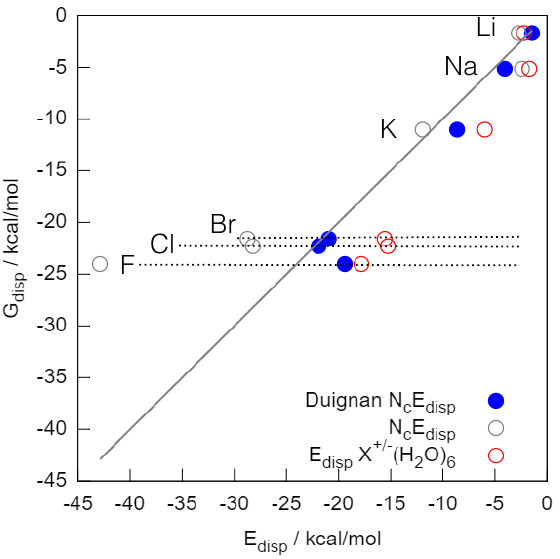
\includegraphics[width=0.8\linewidth]{images/ct_main/duignan_disp.png}
 \end{center}
 \caption[Ion/water dispersion energies and non-linear scaling]{\label{fig:duignan_disp}Figure adapted from Duignan et al.\cite{duignan2014collins}. 
 Figure highlights the non-linear scaling of interaction energy components, both N$_{c}$E$_{disp}$ estimates are too large to fit the continuum
 model described in the same reference. The SAPT2+3(CCD) results for explicitly modeled larger clusters I present here underestimate the dispersion 
 energy relative to the higher order estimate of G$_{disp}$ and so is the more physically consistent result. This demonstrates that interaction 
 energy components are not additive even within the first solvation shell. N$_{c}$ are experimental coordination numbers and E$_{disp}$ are dispersion
 energies from DFT-SAPT or SAPT2+3(CCD) depending on source.}
\end{figure}

  A term often left out of discussions of the SAPT interaction energy is the exchange component which is evaluated with an approximation
  in Psi4 that scales with the square of the overlap integral between basis functions centered on the separate monomers. This property allows for a quantitative 
  assessment of the degree of charge overlap within the clusters and is seen to track the charge transfer values from AIM in Table \ref{tab:ct_all} reasonably 
  well. A charge transfer component of the SAPT induction energy can be separated from polarization using one of the two methods discussed in Ref. \cite{stone2009ct} 
  and Ref. \cite{jeziorski2004regsapt,misquitta2013regsapt}. I discuss more on this later as well.

  The energetic analysis is complemented here with QTAIM descriptors highlighted in Table \ref{tab:dimer_aim}. As with the SAPT energies, each of the properties
  correlates with the strongly ionic/electrostatic nature of ion/water association (positive $\nabla\sur{2}\rho$ at the bond critical point (\emph{bcp}) and a 
  ratio of the magnitude of the largest attractive curvature to the repulsive curvature, $\frac{\left|\lambda\sous{1}\right|}{\lambda\sous{3}}$, less than unity). 
  However hydrogen-bonding within the AIM theory is characterized by an electrostatic presentation of the electron density curvature but a negative total energy
  density which is dominated by the potential energy density. This differs from a covalent linkage which  would also have a negative second derivative at the 
  \emph{bcp}. The large amount of electron density ($\rho$) located at the F\sur{-}(H\sous{2}O) dimer \emph{bcp} coupled with the negative total energy per charge
  is consistent with the uncharacteristically high induction and exchange contributions to the SAPT interaction energies relative to Cl\sur{-} and Br\sur{-}. This
  may offer some insight into the origin of the argument for the apparent chemical character of the interaction discussed in Refs. 
  \cite{collins2007review,mccoy2006prywaterf}. 
  
  It is evident that the F\sur{-} ion is much more strongly associated with the water than are the other halides likely owing to its small size and relatively 
  large proton affinity\cite{kim2002bigall}. This is also seen through the extent of charge penetration of the ion into the water ``electron cloud.'' I found 0.79 
  Bohr separation of the ion from the \emph{bcp} as compared to 1.32 and 1.43 Bohr for Cl\sur{-} and Br\sur{-}, respectively. However, an AIM analysis of a series 
  of halogen and hydrogen bonded complexes together with the reduced variational space (RVS) energy decomposition analysis (at the SCF level) revealed that the 
  decrease in the total energy density and increasing electron density at the intermolecular \emph{bcp} are principally due to a marked increase in attractive
  electrostatic interactions\cite{angelina2013cov}. In the RVS theory, charge transfer is considered a component of the chemical or covalent energy terms.

\begin{table}
 \begin{center}
 \begin{tabular}{cccccrc}
  \multicolumn{1}{c}{Ion} & \multicolumn{1}{c}{r(H\sous{2}O-\emph{bcp})} & \multicolumn{1}{c}{$\rho$} & \multicolumn{1}{c}{$\nabla^2\rho$} & \multicolumn{1}{c}{$\left|\lambda_{1}\right|/\lambda_{3}$} & \multicolumn{1}{c}{$H$/$\rho$} & \multicolumn{1}{c}{$\left|V\right|$/G} \tabularnewline
 \hline
  Li$^+$ & 2.16 & 0.0367 & 0.2984 & 0.17 &  0.3229 & 0.81 \tabularnewline
  Na$^+$ & 2.31 & 0.0249 & 0.1865 & 0.14 &  0.3212 & 0.79 \tabularnewline
  K$^+$  & 2.40 & 0.0213 & 0.1137 & 0.15 &  0.2101 & 0.81 \tabularnewline
  F$^-$  & 0.79 & 0.0882 & 0.1351 & 0.38 & -0.4848 & 1.56 \tabularnewline
  Cl$^-$ & 1.32 & 0.0291 & 0.0589 & 0.28 & -0.1456 & 1.22 \tabularnewline
  Br$^-$ & 1.43 & 0.0238 & 0.0472 & 0.26 & -0.1042 & 1.17 \tabularnewline
 \hline
 \end{tabular}
 \end{center}
 \caption[Atoms in molecules properties at \emph{bond critical point}]{\label{tab:dimer_aim} AIMAll output of several chemical indicators computed 
 at the intermolecular bond critical point (\emph{bcp}). 
 r(H\sous{2}O-\emph{bcp}) is the distance from the participating atom in the water molecule to the intermolecular \emph{bcp} and is a 
 measure of ion penetration. $\rho$ is the value of the density and $\nabla\sur{2}\rho$ the Laplacian at the \emph{bcp}. In the fourth 
 column, we report the ratio of the largest negative curvature (attraction) to the curvature along the bond path (repulsion). This is 
 typically interpreted as a measure of the local balance between potential and kinetic energies and is usually much less than unity for
 closed-shell, primarily electrostatic interactions. Additionally, we report the total energy density per unit charge and the ratio of 
 the potential to kinetic energy at the critical point. Hydrogen bonds in the AIM theory display largely electrostatic character in the
 Laplacian but somewhat chemical character in the energy terms. It is the uncharacteristically high amount of charge and enormously 
 negative total energy density which may fuel speculation that F\sur{-}/water interactions possess some chemical character. All  values 
 are reported in atomic units.}
\end{table}

  My discussion on charge transfer (or delocalization) in ion/water dimers focuses on the data presented in Table \ref{tab:dimer_ct}. 
  The sign convention used here is that charge depletion is given a negative value and accumulation a positive one. The data indicated that there was a loss 
  of charge for anions and an accumulation in the virtual orbitals of each of the cations. In the anion/water dimer, charge is also lost by the ion-bound hydrogen 
  (H\sous{b}) and populates a \emph{p}-state centered on the oxygen and also a diffuse Rydberg state bridging the oxygen and trailing hydrogen (resembling
  $\frac{1}{2}$ the lowest unoccupied molecular orbital, LUMO). 

\begin{table}
 \begin{center}
 \begin{tabular}{lrlrlrlrlrlr}
  A & $\delta$q(A) & A & $\delta$q(A) & A & $\delta$q(A) & A & $\delta$q(A) & A & $\delta$q(A) & A & $\delta$q(A) \tabularnewline
 \hline
  Li\sur{+} &  32.4 & O         &  117.0 & Na\sur{+} &  27.4 & O         &  86.2 & K\sur{+}  &  21.9 & O         &  68.3 \tabularnewline
            &       & H\sous{1} &  -74.7 &           &       & H\sous{1} & -56.8 &           &       & H\sous{1} & -45.1 \tabularnewline
            &       & H\sous{2} &  -74.7 &           &       & H\sous{2} & -56.8 &           &       & H\sous{2} & -45.1 \tabularnewline
  F\sur{-}  & -83.4 & O         &  191.3 & Cl\sur{-} & -62.1 & O         & 110.0 & Br\sur{-} & -62.5 & O         &  98.5 \tabularnewline
            &       & H\sous{b} & -174.3 &           &       & H\sous{b} & -77.3 &           &       & H\sous{b} & -60.7 \tabularnewline
            &       & H\sous{f} &   66.3 &           &       & H\sous{f} &  29.3 &           &       & H\sous{f} &  24.7 \tabularnewline
 \hline
 \end{tabular}
 \end{center}
 \caption[Atoms in molecules atomic charges for ion/water dimers]{\label{tab:dimer_ct} AIM-derived charge transfer values (in m\emph{e}, millielectrons) 
 for dimers computed with AIMAll. Negative values reflect charge loss, positive values reflect charge accumulation.}
\end{table}
  
  \noindent These features are illustrated in the electron density difference maps of Figures \ref{fig:f-6-r4aa-delrho}
  and \ref{fig:f-2-contour}. The oxygen amasses charge also in the cation/water dimers, drawing equal quantities of charge from the dangling hydrogens. About one 
  half of the charge exchanged in the weakest anion/water dimers (Cl\sur{-} and Br\sur{-}) is exchanged by even the most strongly bound cation/water dimer 
  (Li\sur{+}). These results compare well to the values obtained by Soniat et al. for Na\sur{+}, K\sur{+}, and Cl\sur{-}\cite{soniat2012ct}and we agree 
  qualitatively with trends which conclude charge transfer increases in the order of Br\sur{-} $<$ Cl\sur{-} $<$ F\sur{-} originating from studies
  of CT in halide/water dimers with L\"{o}wdin and natural bond orbital (NBO) charges\cite{kim1999bigf,kim2000smallall,kim2002bigall,hynes2000cthalides}. 

\begin{figure}
 \begin{center}
  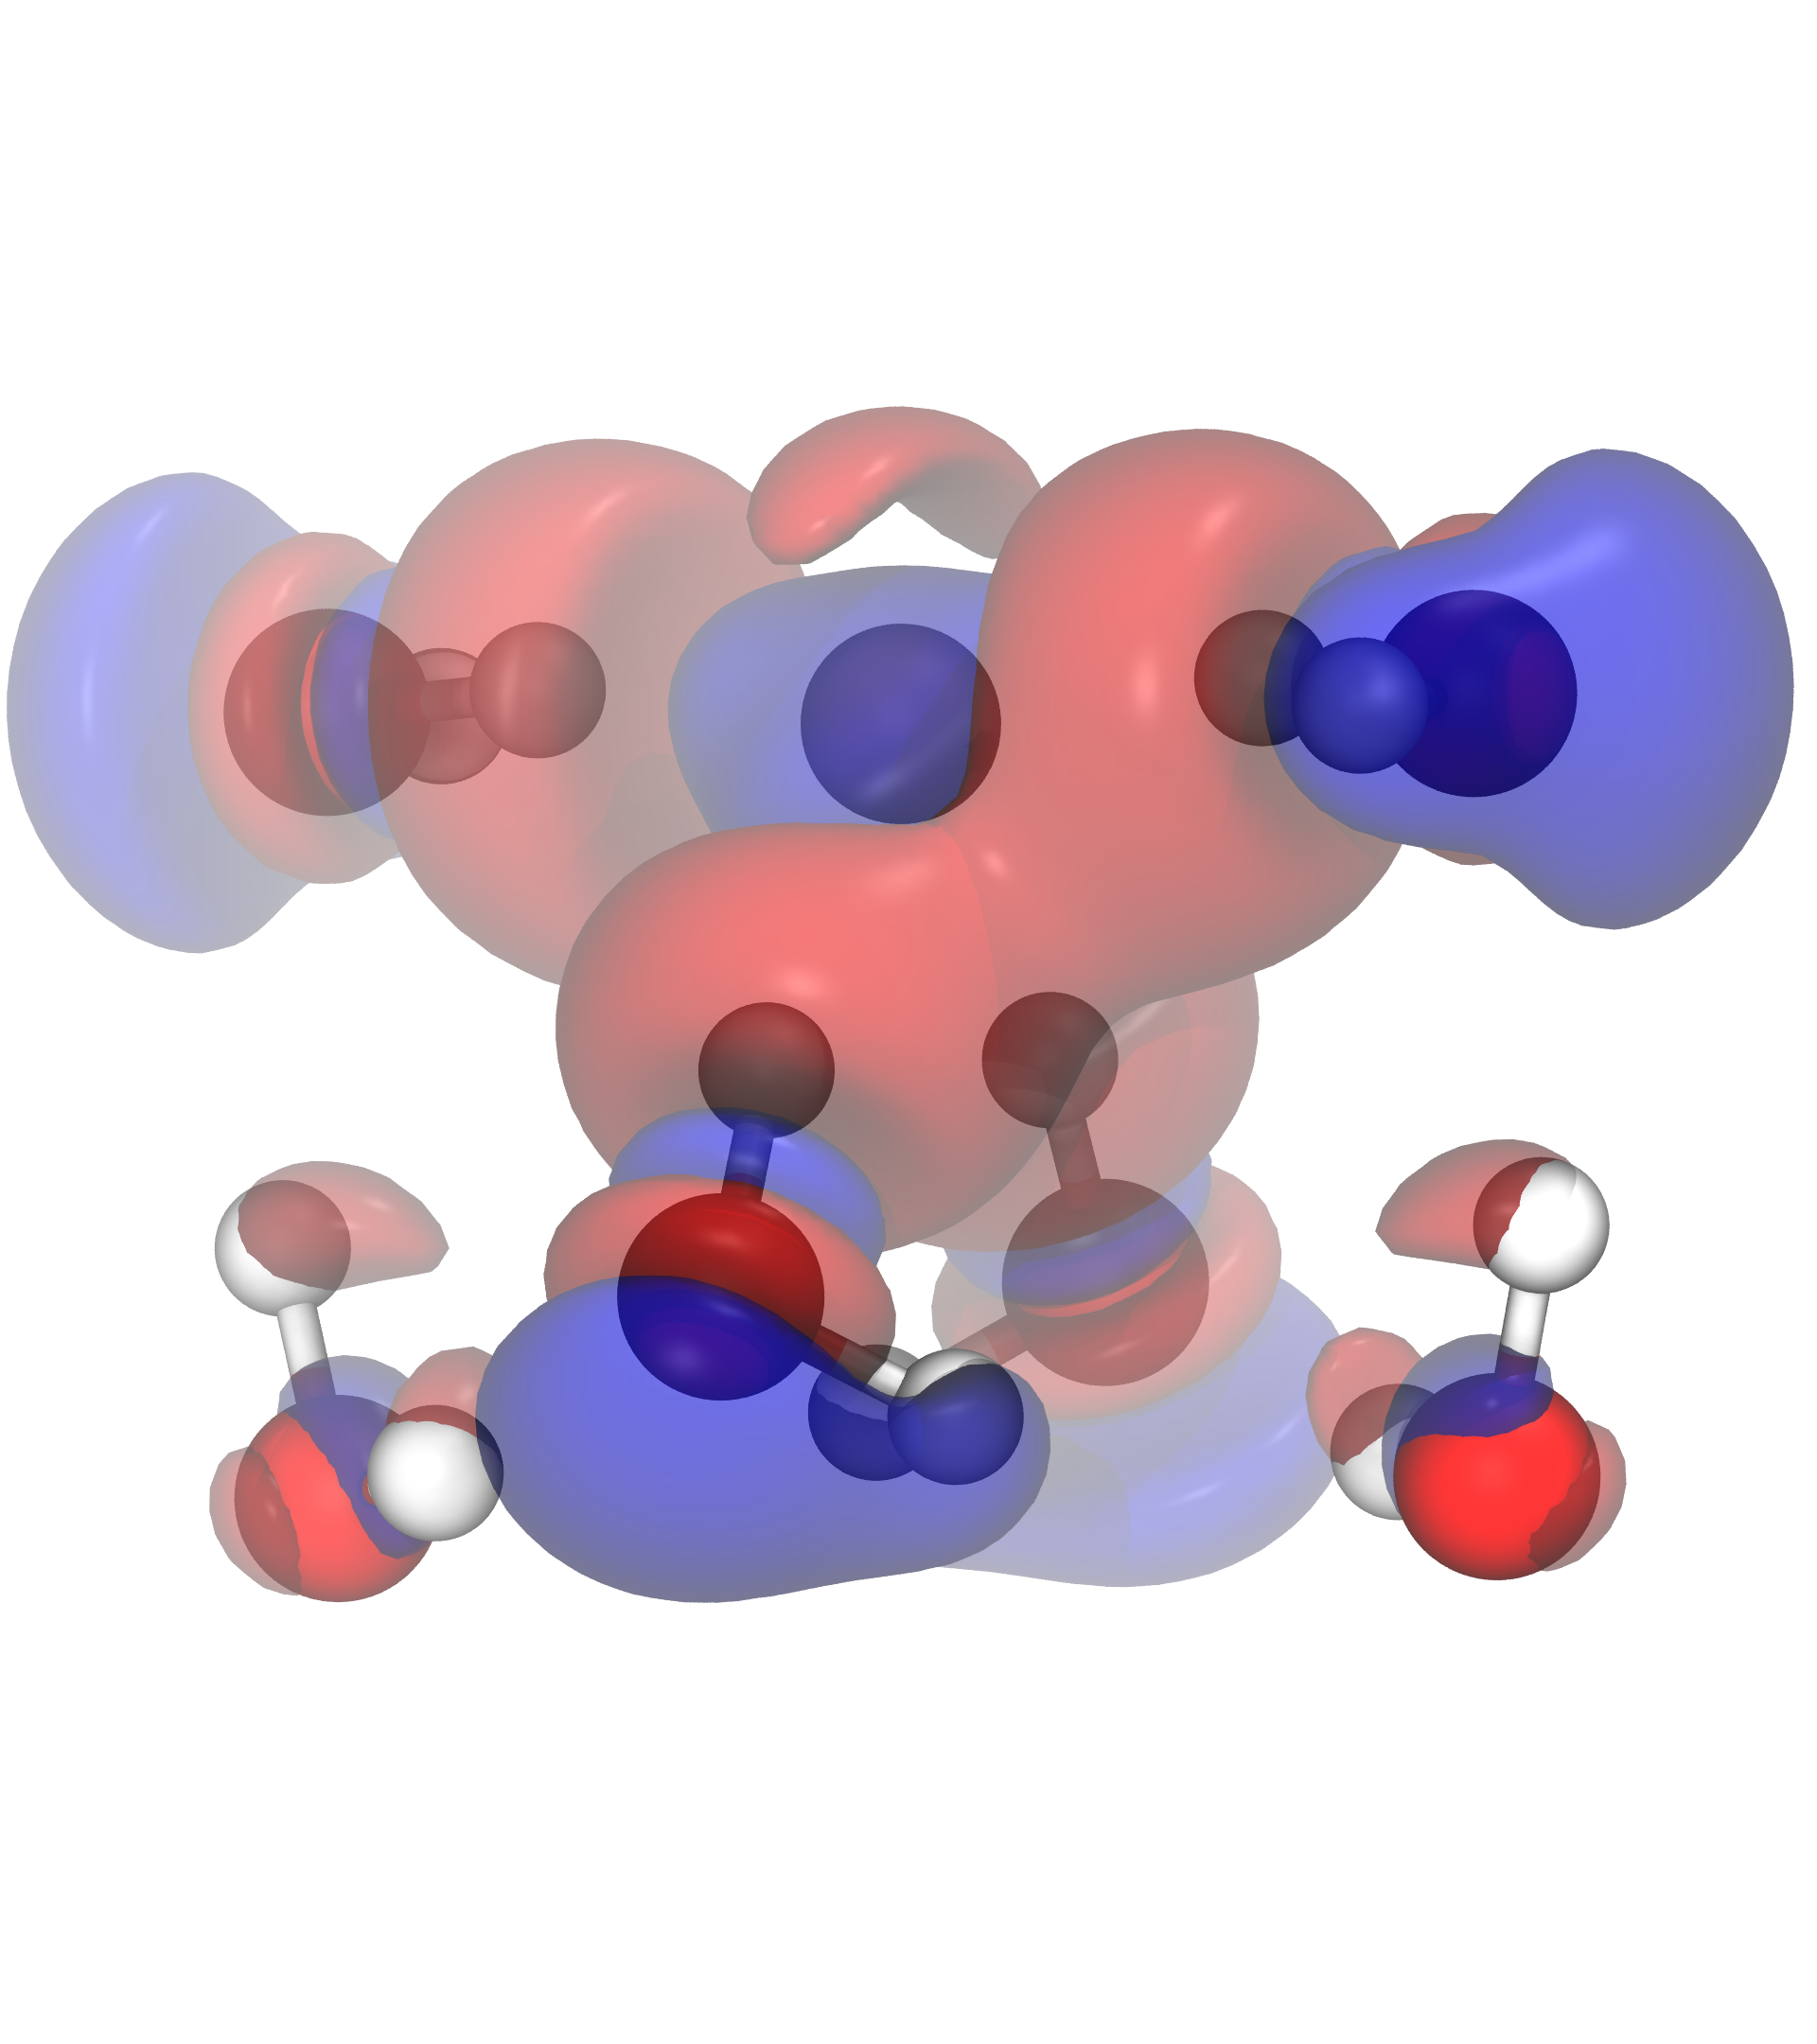
\includegraphics[width=0.98\linewidth]{images/ct_main/f-6-r4aa.png}
 \end{center}
 \caption[Electron density difference map in F$^{-}$(H$_{2}$O)$_{6}$]{\label{fig:f-6-r4aa-delrho}An electron density difference map of the $\pm$0.0022 \emph{e}
 isosurfaces of one of the F$^{-}$(H$_{2}$O)$_{6}$ clusters.}
\end{figure}

\begin{figure}
 \begin{center}
  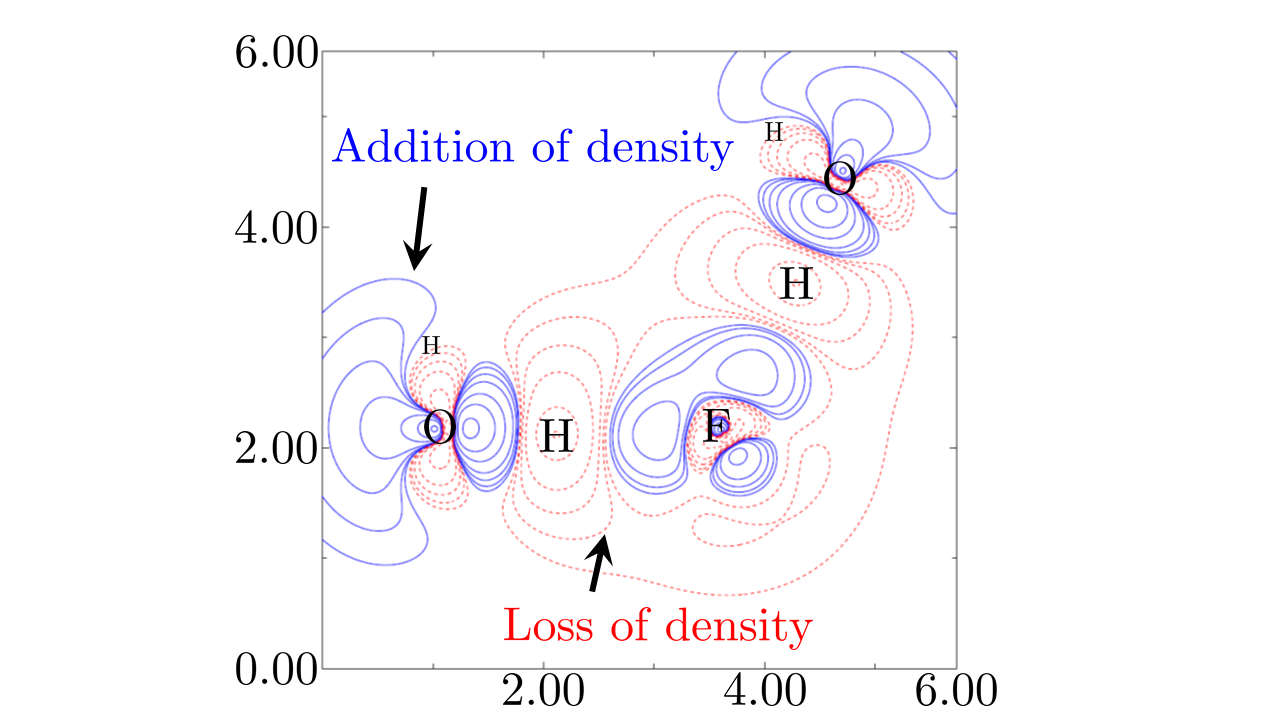
\includegraphics[width=0.98\linewidth]{images/ct_main/f-2-deltarho-Hb1XHb2.jpg}
 \end{center}
 \caption[Electron density difference contours in F$^{-}$(H$_{2}$O)$_{2}$]{\label{fig:f-2-contour}An electron density difference contour map of 
 F$^{-}$(H$_{2}$O)$_{2}$ clusters showing regions of charge accumulation and depletion.}
\end{figure}

  Moving beyond dimers into clusters, I'll be referring to Table \ref{tab:ct_all}. For trimers, there is a notable increase
  in the amount of charge redistribution throughout the system which falls well short of a doubling of the result for the dimers. Competition between ion/water
  versus water/water is not seen until reaching a coordination number of \emph{n} $=$ 3. We also point out that the trend observed for the anion/water dimers, 
  namely that charge transferred increases in the order Br\sur{-} $<$ Cl\sur{-} $<$ F\sur{-}, is in danger of reversing as the effect for F\sur{-} appears to 
  saturate rather quickly. This transition in anions is consistent with a study by Patel et al. in which they've found that for F\sur{-}/water clusters up to 
  \emph{n} $=$ 3, the ion polarizability was somewhat enhanced relative to the gas phase F\sur{-} polarizability\cite{patel2010polarizability}. Beyond a cluster 
  size of \emph{n} $=$ 3, the ion polarizability was reduced relative to the gas phase and as a consequence the observed ion-to-solvent transfer is quickly exhausted. 
  Figure \ref{fig:f-6-r4aa-delrho} shows that the water distorts the electron density of the ion towards poles directed at neighboring hydrogens. These polarized 
  electron-rich clouds are simply more willing to relinquish their charge from softer ions like Cl\sur{-} and Br\sur{-} than harder ones like F\sur{-}; and we 
  note that all anions eventually see a decrease in polarizability in the condensed phase limit -- a conclusion also reached by Masia\cite{masia2009polarize,masia2013polar} 
  and other researchers, see page 4 of Ref. \cite{ren2003amoeba} and the related discussion for more references.

  In clusters with more than 3 waters we see very little in the way of change from cation/water systems, maintaining a steady 60 to 80 millielectron draw from
  surrounding waters with a general preference for arrangements producing a high symmetry and maximizing the number of direct ion/water contacts. The same trend
  we observed for dimers is preserved in the micro-solvated states with Li\sur{+} drawing more charge than Na\sur{+} and K\sur{+}. However, the anion trend has
  reversed with Br\sur{-} shedding up to about 170 millielectrons while F\sur{-} has lost around 150 millielectrons at most. These figures are similar to the 
  results from Zhao, Rogers, and Beck where they found Cl\sur{-} to lose about 200 millielectrons\cite{rogers2010ctpolar}. Their calculations included the dipole 
  and quadrupole field of waters beyond the first hydration shell suggesting there may be a small amount of additional charge displaced as we approach the bulk
  limit. Finally, we note that the amounts of charge exchanged between the ions and water, just as we saw for the energies, did not increase linearly with each
  additional water -- in fact, most of these figures barely doubled with the addition of 5 more waters!

\begin{table}
 \begin{center}
  \begin{tabular}{lrlrlr}
   Cluster & $\delta$q(X\sur{\pm}) & Cluster & $\delta$q(X\sur{\pm}) & Cluster & $\delta$q(X\sur{\pm})\tabularnewline
  \hline
   \tabularnewline
   \multicolumn{2}{c}{\textbf{X\sur{\pm}(H\sous{2}O)\sous{1-4}}} & \multicolumn{2}{c}{\textbf{X\sur{\pm}(H\sous{2}O)\sous{4-5}}} & \multicolumn{2}{c}{\textbf{X\sur{\pm}(H\sous{2}O)\sous{5-6}}}\tabularnewline
   \tabularnewline
Li\sur{+} C\sous{2v}      &  32.4& F\sur{-} C\sous{1}                   &-138.7& Br\sur{-} R4A1             &-163.1 \\
Na\sur{+} C\sous{2v}      &  27.4& F\sur{-} C\sursous{\prime\prime}{1}  &-139.7& Br\sur{-} R4A              &-159.4 \\
K\sur{+} C\sous{2v}       &  21.9& F\sur{-} C\sous{4}                   &-134.6& Br\sur{-} R43f             &-157.8 \\
F\sur{-} C\sous{1}        & -83.4& F\sur{-} 3+1(C\sous{s})              &-139.2& Br\sur{-} R3AA\sur{\prime} &-162.3 \\
Cl\sur{-} C\sous{1}       & -62.1& Cl\sur{-} C\sursous{\prime}{1}       &-144.6& Br\sur{-} R5               &-149.4 \\
Br\sur{-} C\sous{1}       & -62.5& Cl\sur{-} C\sursous{\prime\prime}{1} &-143.0& Br\sur{-} R4f3             &-156.1 \\
                          &      & Cl\sur{-} C\sous{4}                  &-135.3&                            &       \\
Li\sur{+} D\sous{2d}      &  58.9& Br\sur{-} C\sursous{\prime}{1}       &-150.9& Li\sur{+} D\sous{2d}       &  82.0 \\
Na\sur{+} D\sous{2d}      &  49.7& Br\sur{-} C\sursous{\prime\prime}{1} &-149.1& Li\sur{+} 4+2(C\sous{s})   &  82.5 \\
K\sur{+} D\sous{2d}       &  37.6& Br\sur{-} C\sous{4}                  &-139.4& Li\sur{+} C\sous{2}        &  82.2 \\
F\sur{-} C\sous{2}        &-117.4&                                      &      & Na\sur{+} D\sous{2d}       &  77.2 \\
Cl\sur{-} C\sous{1}       &-100.0& Li\sur{+} C\sous{2}                  &  74.7& Na\sur{+} 4+2(C\sous{s})   &  76.9 \\
Br\sur{-} C\sous{1}       &-101.5& Li\sur{+} 4+1(C\sous{2})             &  82.4& Na\sur{+} C\sous{2}        &  74.7 \\
                          &      & Na\sur{+} C\sous{2}                  &  77.1& K\sur{+} D\sous{2d}        &  63.9 \\
Li\sur{+} D\sous{3}       &  74.4& Na\sur{+} 4+1(C\sous{2})             &  76.9& K\sur{+} 4+2(C\sous{s})    &  64.3 \\
Li\sur{+} 2+1(C\sous{2v}) &  58.6& K\sur{+} 4+1(C\sous{2})              &  62.6& K\sur{+} C\sous{2}         &  61.5 \\
Na\sur{+} D\sous{3}       &  65.4& K\sur{+} C\sous{2}                   &  59.0& F\sur{-} L3L3              &-150.9 \\
Na\sur{+} 2+1(C\sous{2v}) &  50.3& K\sur{+} 4+1(C\sous{1})              &  57.2& F\sur{-} R3ADA             &-145.7 \\
K\sur{+} D\sous{3}        &  51.5& F\sur{-} R3L2                        &-140.5& F\sur{-} R4AA              &-142.1 \\
K\sur{+} 2+1(C\sous{2v})  &  42.3& F\sur{-} R4L                         &-140.9& F\sur{-} Bf\sur{\prime}    &-140.0 \\
F\sur{-} C\sous{3}        &-128.4& F\sur{-} L3DL                        &-141.3& F\sur{-} R3AAL             &-141.6 \\
F\sur{-} 2+1(C\sous{s})   &-124.0& F\sur{-} R4A                         &-138.1& F\sur{-} Bf                &-138.9 \\
Cl\sur{-} C\sous{3}       &-121.1& F\sur{-} R43f                        &-137.4& Cl\sur{-} R4AA             &-163.8 \\
Cl\sur{-} 2+1(C\sous{s})  &-119.5& F\sur{-} R4L\sur{\prime}             &-141.4& Cl\sur{-} Bf\sur{\prime}   &-159.3 \\
Br\sur{-} C\sous{3}       &-124.2& F\sur{-} R3AA                        &-140.0& Cl\sur{-} Bf               &-158.7 \\
Br\sur{-} 2+1(C\sous{s})  &-123.1& Cl\sur{-} R4A1                       &-155.5& Cl\sur{-} Bd               &-150.6 \\
                          &      & Cl\sur{-} R4A                        &-151.2& Cl\sur{-} Bd\sur{\prime}   &-151.3 \\
Li\sur{+} S\sous{4}       &  81.2& Cl\sur{-} R43f                       &-150.0& Br\sur{-} R4AA             &-174.2 \\
Li\sur{+} 3+1(C\sous{2})  &  75.8& Cl\sur{-} R3AA\sur{\prime}           &-154.5& Br\sur{-} Bf\sur{\prime}   &-168.8 \\
Na\sur{+} S\sous{4}       &  76.0& Cl\sur{-} R5                         &-144.0& Br\sur{-} Bf               &-168.2 \\
Na\sur{+} 3+1(C\sous{2})  &  66.6& Cl\sur{-} R3AA                       &-149.4& Br\sur{-} Bd               &-158.2 \\
K\sur{+} S\sous{4}        &  61.4& Cl\sur{-} R4f3                       &-149.6& Br\sur{-} Bd\sur{\prime}   &-159.3 \\
K\sur{+} 3+1(C\sous{2})   &  53.5&                                      &      &                            &       \\
  \hline 
  \end{tabular}
 \end{center}
 \caption[Atoms in molecules partial charges on ions in all clusters]{\label{tab:ct_all} Charge transfer to ($\delta$q $>$ 0) or from 
 ($\delta$q $<$ 0) the ion measured in millielectrons for each complex examined. Note the increases are not linear when additional 
 waters are considered and the $\delta$q to cations and from F\sur{-} has already nearly plateaued when considering just the first 
 hydration shell.}
\end{table}

  An alternative approach to quantifying the amount of charge transfer was described by Belpassi and coworkers\cite{belpassi2009cd1,belpassi2010cd2} and is 
  particularly suited to examining charge displacement in or between linear or planar molecules. By slicing a cube file of the electron density difference 
  upon complexation into many planes perpendicular to the bond between the ion and nearest water atom and then integrating, I can examine the amount of charge
  transferred from one side of the plane to the other (direction depends on direction of integration, -z to +z or +z to -z). Belpassi has argued that between two
  interacting molecules there will be a minimum or a maximum in the curve which is the estimate of total charge transferred. Figure \ref{fig:belpassi} shows the
  charge displacement curve for all the ion/water dimers. The integration proceeds from -x to +x and so a positive value like we obtain for cations indicates 
  charge flow from the left side to the right (ion to water) and vice versa for negative values like that obtained for anions. The hills and valleys in this 
  curve coincide with the pattern of density accumulation or depletion like what is seen in Figure \ref{fig:f-2-contour} and provide an insightful new 
  perspective. Charge transfer values from this plot are as follows: 10.1 (Li\sur{+}), 10.1 (Na\sur{+}), 27.3 (K\sur{+}), 72.6 (F\sur{-}), 49.3 (Cl\sur{-}), 
  and 46.9 (Br\sur{-}) millielectrons which reverses the cation trend from that observed with AIM-derived partial charges but preserves the trend for anions.
  
\begin{figure}
 \begin{center}
  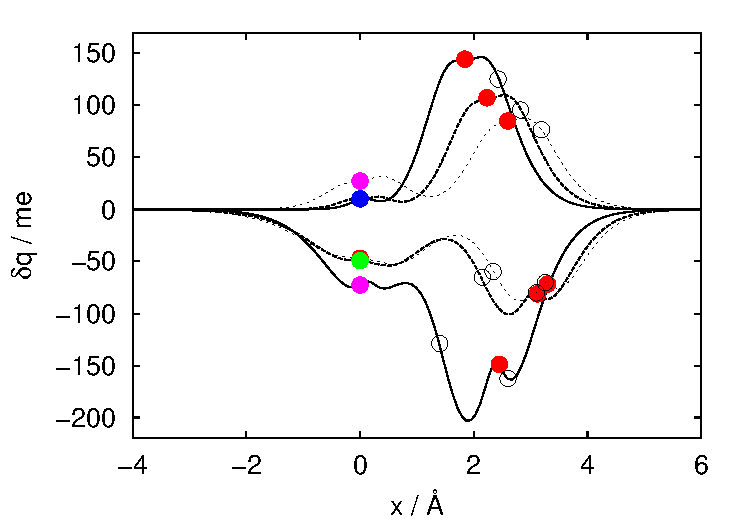
\includegraphics[width=0.98\linewidth]{images/ct_main/belpassi.pdf}
 \end{center}
 \caption[Charge displacement curves for ion/water dimers]{\label{fig:belpassi}Charge displacement curves following Refs. \cite{belpassi2009cd1,belpassi2010cd2}. 
  The curve indicates both direction and magnitude of charge passing through a moving plane perpendicular to the ion-water bond and so offers a unique
  perspective of charge redistribution in the dimers. Refs. \cite{belpassi2009cd1,belpassi2010cd2} and citations therein argue that an unambiguous 
  estimation of the charge transferred can be evaluated at the minimum/maximum appearing in the curve between the ion and the nearest water atom positions.
  The integration proceeds from left to right and so a positive value like we obtain for cations indicates charge flows from the right side to the 
  left (water to ion) and vice versa for negative values like those obtained for anions. All ions are located at x=0. Red and white circles not at
  the x=0 coordinate signify oxygen and hydrogen positions, respectively. Ions are colored magenta (F\sur{-}), green (Cl\sur{-}), red (Br\sur{-}), 
  larger red (Li\sur{+}), blue (Na\sur{+}), and magenta (K\sur{+}).}
\end{figure}
  
  \subsection{\label{ch3:sec2:level1:chasm2}Energy stabilization due to charge transfer}
  Tables \ref{tab:small_clust} and \ref{tab:3_clust} highlight the significant enhancement in basis set independence that regularization affords.
  Charge transfer energies are reported for basis sets ranging from a double-$\zeta$ through to a quadruple-$\zeta$ quality, yet exhibit little
  variance. This consistency is maintained as additional waters are added to create high or even low symmetry arrangements (see also Tables 
  \ref{tab:small_clusters}--\ref{tab:6_clusters}, with (X\sur{\pm}(H\sous{2}O)\sous{n}; \emph{n} = 1, \dots, 6)). However, there's an issue with
  these figures that was also observed by Lao et al.\cite{lao2016cdftsapt}. The cation/water dimers are considered to be a trivial case, with 
  the strength of polarization and charge transfer interactions increasing in the order of K\sur{+} < Na\sur{+} < Li\sur{+}, complimenting the
  decrease in ion/water distance. However, CT\sursous{(2)}{SM09}, CT\sursous{(2)}{Reg, aDZ}, and CT\sursous{(2)}{Reg, pc1} displayed a tendency
  to go positive for small cation/water clusters and only slightly negative for the largest clusters. This is with the exception of Na\sur{+} which
  always produced a positive charge transfer energy, regardless of cluster size, method, or basis set used. Ordering of the cation energies using
  the SM09 method trend varied with cluster size but remained constant among regularized energies as K\sur{+} > Na\sur{+} > Li\sur{+} (where K\sur{+} 
  is merely the least \emph{unfavorable}). It's also interesting to note that while Li\sur{+}/water and K\sur{+}/water energies became more negative 
  with increasing cluster size, the regularized energies increased.
  
\begin{table}
 \begin{center}
  \begin{tabular}{lcccccc}
   \hline
   \hline
    Cluster & CT\sursous{(2)}{Reg, aDZ} & CT\sursous{(2)}{Reg, pc1} & CT\sursous{(2)}{Reg, aTZ} & CT\sursous{(2)}{Reg, pc2} & CT\sursous{(2)}{Reg, dTZ} & CT\sursous{(2)}{Reg, dQZ} \tabularnewline
   \hline
    \tabularnewline
    \multicolumn{7}{c}{\textbf{X\sur{\pm}(H\sous{2}O)}}  \tabularnewline
    \tabularnewline
    Li\sur{+} C\sous{2v} & 1.38 & 1.28 & 1.58 & 1.53 & 1.59 & 1.58 \tabularnewline
    Na\sur{+} C\sous{2v} & 0.45 & 0.33 & 0.51 & 0.49 & 0.46 & 0.50 \tabularnewline
    K\sur{+}  C\sous{2v} & 0.06 & 0.04 & 0.06 & 0.05 & 0.06 & 0.06 \tabularnewline
    F\sur{-}  C\sous{1}  &-4.15 &-4.20 &-4.10 &-4.24 &-4.14 &-4.09 \tabularnewline
    Cl\sur{-} C\sous{1}  &-0.67 &-0.70 &-0.62 &-0.62 &-0.62 &-0.60 \tabularnewline
    Br\sur{-} C\sous{1}  &-0.50 &-0.52 &      &-0.46 &-0.45 &-0.44 \tabularnewline

    \tabularnewline
    \multicolumn{7}{c}{\textbf{X\sur{\pm}(H\sous{2}O)\sous{2}}}  \tabularnewline
    \tabularnewline
    Li\sur{+} D\sous{2d} & 2.11 & 2.11 & 2.35 & 2.31 & 2.36 & 2.34 \tabularnewline
    Na\sur{+} D\sous{2d} & 0.83 & 0.65 & 0.91 & 0.88 & 0.86 & 0.90 \tabularnewline
    K\sur{+}  D\sous{2d} & 0.18 & 0.14 & 0.18 & 0.17 & 0.17 & 0.17 \tabularnewline
    F\sur{-}  C\sous{2}  &-4.70 &-4.77 &-4.59 &-4.77 &-4.63 &-4.57 \tabularnewline
    Cl\sur{-} C\sous{1}  &-1.10 &-1.15 &-1.01 &-1.02 &-1.01 &-1.00 \tabularnewline
    Br\sur{-} C\sous{1}  &-0.84 &-0.88 &      &-0.77 &-0.76 &-0.75 \tabularnewline
   \hline
   \hline
  \end{tabular}
 \end{center}
 \caption[Charge transfer energies for ion/water clusters with \emph{n} = 1 and 2]{\label{tab:small_clust} Charge transfer energies from regularized 
 SAPT computed (by column) with the (aug-)cc-pVDZ, (aug-)pc-1, (aug-)cc-pVTZ, (aug-)pc-2, 
 def2-TZVPP(D), and def2-QZVPP(D) basis sets. All values expressed in kcal/mol. Some entries are left blank due to limitations with the software.}
\end{table}

\begin{table}
 \begin{center}
  \begin{tabular}{lcccccc}
   \hline
   \hline
    Cluster & CT\sursous{(2)}{Reg, aDZ} & CT\sursous{(2)}{Reg, pc1} & CT\sursous{(2)}{Reg, aTZ} & CT\sursous{(2)}{Reg, pc2} & CT\sursous{(2)}{Reg, dTZ} & CT\sursous{(2)}{Reg, dQZ} \tabularnewline
   \hline
    \tabularnewline
    \multicolumn{7}{c}{\textbf{X\sur{\pm}(H\sous{2}O)\sous{3}}}  \tabularnewline
    \tabularnewline
    Li\sur{+} 2+1(C\sous{2}) & 2.20 &  2.13 & 2.41 & 2.36 & 2.43 & 2.41 \tabularnewline
    Li\sur{+} D\sous{3}      & 2.27 &  2.24 & 2.50 & 2.46 & 2.52 & 2.50 \tabularnewline 
    Na\sur{+} 2+1(C\sous{2}) & 0.85 &  0.69 & 0.93 & 0.90 & 0.88 & 0.92 \tabularnewline
    Na\sur{+} D\sous{3}      & 1.03 &  0.83 & 1.12 & 1.08 & 1.07 & 1.11 \tabularnewline
    K\sur{+}  2+1(C\sous{2}) & 0.10 &  0.08 & 0.11 & 0.10 & 0.10 & 0.10 \tabularnewline
    K\sur{+}  D\sous{3}      & 0.24 &  0.22 & 0.25 & 0.24 & 0.24 & 0.25 \tabularnewline
    F\sur{-}  2+1(C\sous{s}) &-5.34 & -5.41 &-5.24 &-5.42 &-5.29 &      \tabularnewline
    F\sur{-}  C\sous{3}      &-4.31 & -4.38 &-4.18 &-4.33 &-4.21 &      \tabularnewline 
    Cl\sur{-} 2+1(C\sous{s}) &-1.48 & -1.55 &-1.39 &-1.39 &-1.38 &      \tabularnewline
    Cl\sur{-} C\sous{3}      &-1.21 & -1.29 &-1.09 &-1.13 &-1.11 &      \tabularnewline
    Br\sur{-} 2+1(C\sous{s}) &-1.15 & -1.20 &      &-1.07 &-1.05 &      \tabularnewline
    Br\sur{-} C\sous{3}      &-0.94 & -1.00 &      &-0.87 &-0.85 &      \tabularnewline
   \hline 
   \hline
  \end{tabular}
 \end{center}
 \caption[Charge transfer energies for ion/water clusters with \emph{n} = 3]{\label{tab:3_clust} Charge transfer energies from regularized SAPT 
 computed (by column) with the (aug-)cc-pVDZ, (aug-)pc-1, (aug-)cc-pVTZ, (aug-)pc-2, 
 def2-TZVPP(D), and def2-QZVPP(D) basis sets. All values expressed in kcal/mol. Some entries are left blank due to limitations with the software.}
\end{table}  

  Tables \ref{tab:small_clusters}--\ref{tab:6_clusters} do however suggest that electron correlation offers a bit of improvement as it was 
  always evaluated to be negative, but surely does not improve the reliability of the results from either method. The infinite-order correction 
  to the induction energies is argued to account for charge transfer effects wrapped up in higher order effects not captured in the 2\sur{nd}-order
  expansion\cite{lande2015cdftct}. As with electron correlation, this drives the CT energies more negative with the exception of Na\sur{+}, for 
  which the $\delta$\sursous{(2)}{HF}(DCBS) term is curiously positive. The same was observed here as well\cite{lao2016cdftsapt}.

  Anions consistently produced more reasonable values and in the proper ordering (from \emph{least} to \emph{most} favorable): Br\sur{-} < 
  Cl\sur{-} < F\sur{-}. Similar to what I observed for the atoms-in-molecules charge populations for the anions, the energies stagnated beyond
  \emph{n} $>$ 3 for F\sur{-} -- however, without falling behind either Cl\sur{-} or Br\sur{-}. CT\sursous{(2)}{SM09} energies hovered around
  twice the energies predicted by the regularized method, especially for larger clusters. This is an interesting result as the saturation in 
  the amount of charge transfer observed particularly for F\sur{-} might have been expected to lead to better agreement between the SM09 and
  reg-SAPT methods.

  These results are also visualized in Figure \ref{fig:ct_energy}. Though here, we are able to decompose the CT energies even further into 
  donor $\rightarrow$ acceptor and donor $\leftarrow$ acceptor contributions (here, donor and acceptor refer to electrons, not 
  protons)\cite{jeziorski1994sapt}. The CT\sur{(2)}(X$\leftarrow$W) values settled near 0. kcal/mol for the entire range of cation/water clusters
  considered. This is to be expected however, as CT\sur{(2)}(X$\leftarrow$W) represents the charge transfer energy change from the water polarizing
  the ion. This leaves only the water-to-ion transfer which appeared to somewhat destabilize these complexes as discussed previously. For the
  anion/water clusters, inductive effects due to charge transfer appeared beneficial in both directions, though with the larger 
  portion originating from the ion $\leftarrow$ water term. As discussed previously, it is apparent that CT\sur{(2)}(X$\leftarrow$W) has saturated 
  for F\sur{-} already by \emph{n} $=$ 3, while both Cl\sur{-} and Br\sur{-} appeared to not yet converge.
  
\begin{figure}
 \begin{center}
  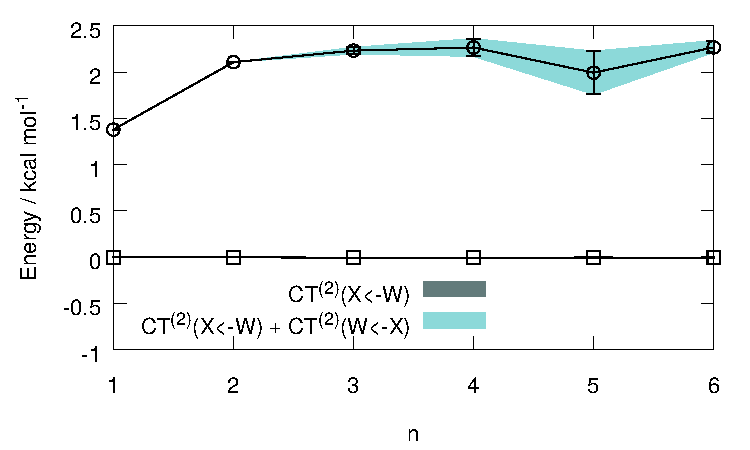
\includegraphics[width=0.48\linewidth]{images/ct_energy_data/e2ind_ct2_plots/pdf/li-ct.pdf}
  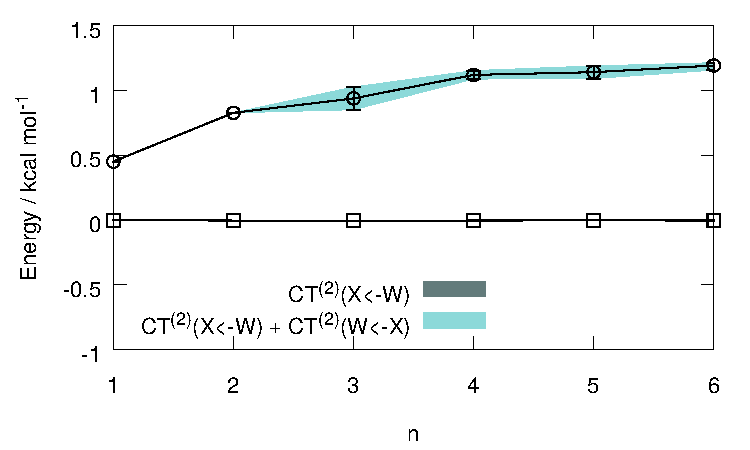
\includegraphics[width=0.48\linewidth]{images/ct_energy_data/e2ind_ct2_plots/pdf/na-ct.pdf} \\
  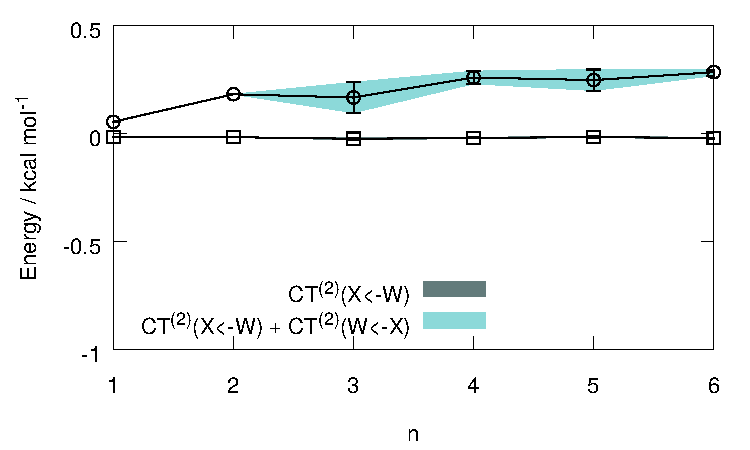
\includegraphics[width=0.48\linewidth]{images/ct_energy_data/e2ind_ct2_plots/pdf/k-ct.pdf} 
  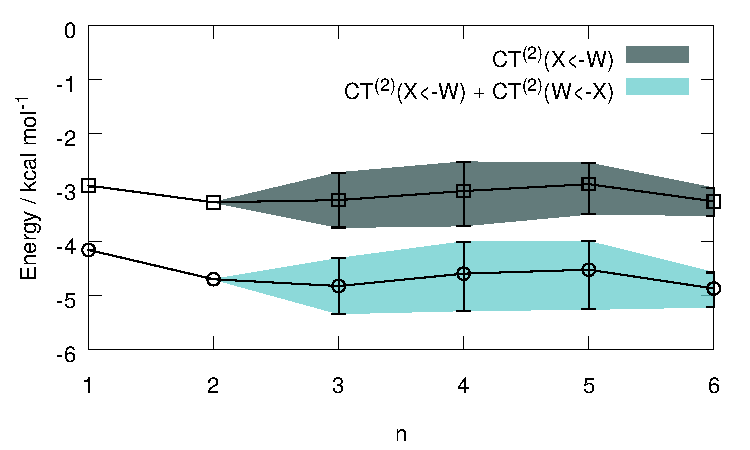
\includegraphics[width=0.48\linewidth]{images/ct_energy_data/e2ind_ct2_plots/pdf/f-ct.pdf} \\
  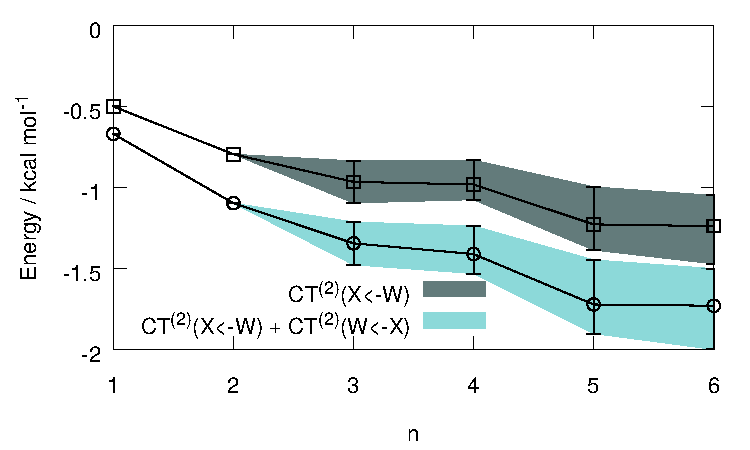
\includegraphics[width=0.48\linewidth]{images/ct_energy_data/e2ind_ct2_plots/pdf/cl-ct.pdf} 
  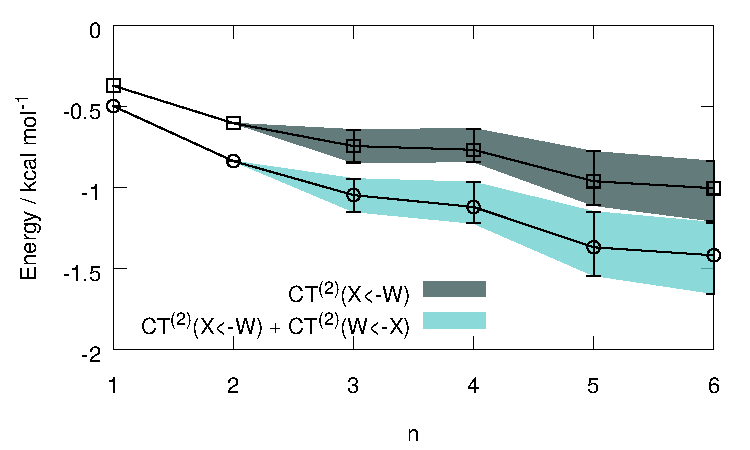
\includegraphics[width=0.48\linewidth]{images/ct_energy_data/e2ind_ct2_plots/pdf/br-ct.pdf} \\
 \end{center}
 \caption[Separate ion and solvent contributions to charge transfer energy]{\label{fig:ct_energy}Ionic and solvent contributions to total 
 charge transfer energies computed with the aug-cc-pVDZ basis set.
 CT\sur{(2)}(X$\leftarrow$W) is the charge transfer energy change for the ion induced by the permanent multipoles of the surrounding 
 solvent. Solvent effects due to the neighboring ion are taken as the difference in CT\sur{(2)}(X$\leftarrow$W) + CT\sur{(2)}(W$\leftarrow$X) 
 and the included ionic contribution. A solid line with points at each coordination number (\emph{n}) traces the mean values across all 
 structures and the shaded region is bounded by the maximum and minimum for a given cluster size. These extrema are identical to those found 
 in Tables 2-5. The procession of the ions from top left to bottom right is as follows: Li\sur{+}, Na\sur{+}, K\sur{+}, F\sur{-}, 
 Cl\sur{-}, and Br\sur{-}.}
\end{figure}

  So why the positive charge transfer energies? Table \ref{tab:liconverge} tells us that for the Li\sur{+}/water dimer, the presence of a regularizing
  potential even in the limit of large $\eta$ more aggressively screens the repulsive contributions than it does the attractive ones. This leads to the 
  systematic overestimation of the repulsive contribution, which may make this method more promising as an upper bound of the polarization energy instead 
  of an estimate of the charge transfer energy.
  
\begin{table}
 \begin{center}
 \resizebox{\columnwidth}{!}{
  \begin{tabular}{cccccccccc}
   \hline
   \hline
    $\eta$   & E\sursous{(2)}{tot,r} & E\sursous{(2)}{tot,r}(Reg) & CT\sur{(2)} & E\sursous{(2)}{ind,r} & E\sursous{(2)}{ind,r}(Reg) & CT\sursous{(2)}{attr} & E\sursous{(2)}{ex-ind,r} & E\sursous{(2)}{ex-ind,r}(Reg) & CT\sursous{(2)}{rep} \tabularnewline
   \hline
    2.0     &-11.43  &-12.54    &1.11  &-19.42  &-14.14   &-5.28    &7.99    &1.60   &6.39 \tabularnewline
    3.0     &-11.43  &-12.81    &1.38  &-19.42  &-15.47   &-3.95    &7.99    &2.66   &5.32 \tabularnewline
    4.0     &-11.43  &-12.82    &1.39  &-19.42  &-16.25   &-3.17    &7.99    &3.42   &4.56 \tabularnewline
    5.0     &-11.43  &-12.77    &1.34  &-19.42  &-16.76   &-2.66    &7.99    &3.99   &4.00 \tabularnewline
    6.0     &-11.43  &-12.70    &1.27  &-19.42  &-17.12   &-2.30    &7.99    &4.42   &3.56 \tabularnewline
    8.0     &-11.43  &-12.56    &1.12  &-19.42  &-17.61   &-1.82    &7.99    &5.05   &2.94 \tabularnewline
    10.0    &-11.43  &-12.44    &1.00  &-19.42  &-17.92   &-1.51    &7.99    &5.48   &2.51 \tabularnewline
    20.0    &-11.43  &-12.08    &0.64  &-19.42  &-18.59   &-0.83    &7.99    &6.51   &1.47 \tabularnewline
    100.0   &-11.43  &-11.60    &0.17  &-19.42  &-19.23   &-0.19    &7.99    &7.62   &0.37 \tabularnewline
    1000.0  &-11.43  &-11.45    &0.02  &-19.42  &-19.40   &-0.03    &7.99    &7.94   &0.04 \tabularnewline
   \hline 
   \hline
  \end{tabular}
  }
 \end{center}
 \caption[Regularized SAPT energy with varying screening width]{\label{tab:liconverge} Illustration of the effect of regularization in SAPT 
 induction energy components for Li\sur{+}(H\sous{2}O) 
 (units of kcal mol\sur{-1}). The exchange part of the interaction is more significantly impacted by the screening potential than is the 
 attractive part -- since CT\sur{(2)} is described nearly exclusively by the polarization of the water molecule, it is seen that the 
 positive CT energy results from the omission of the stresses leading to water-to-ion charge delocalization. Here E\sursous{(2)}{tot,r} is 
 the total induction energy, which is divided in other columns to the attractive induction term and the repulsive exchange coupled term. 
 E\sursous{(2)}{tot,r}(Reg) and CT\sur{(2)} are similarly decomposed. The full CT energy and its components are merely the differences 
 from the two columns preceding it. The table itself was slightly rescaled to fit the dimensions of the page.}
\end{table}

  There is much interest in correlating charge transfer energies in anion/water clusters with the degree of solvation asymmetry in the first 
  hydration shell. While it is known that the softer anions (e.g., Cl\sur{-}, Br\sur{-}, and I\sur{-}) tend to prefer a highly asymmetric 
  first solvation shell, the reduction in polarizability observed in the transition from gas phase to condensed phase for each
  ion\cite{masia2013polar,patel2010polarizability} (presumably from charge transfer to solvent making the ion appear `harder') has been seen to
  decrease solvation anisotropy when modeled with static multipoles using the AMOEBA polarizable force field\cite{rogers2010ctpolar} and the
  polarizable and fluctuating charge model of Soniat et al.\cite{soniat2012ct}. It would be quite useful to observe that semi-/internal bound
  clusters are selected for with enhanced CT energies relative to the surface-bound configurations, see the discussion on this in Ref.
  \cite{kim2002bigall}. Assuming the anion figures to be at least qualitatively accurate, the internal-bound configurations for 
  F\sur{-}(H\sous{2}O)\sous{6} (L3L3, R3AAL, and R3ADA) were selected over the surface bound states by both energy partitioning schemes.
  Perhaps the constrained density functional theory approach of Lande et al.\cite{lande2015cdftct} which showed greater consistency with
  cation/water dimers\cite{lao2016cdftsapt} than the SM09 method or the absolutely localized molecular orbital approach of Khaliullin et 
  al.\cite{khaliullin2008almo} can provide more solid answers using even larger clusters since it is based on DFT.

  This is all not to say that regularized SAPT isn't useful, rather it may be more fitting to interpret these energies in a similar manner to
  the polarized orthogonal local molecular orbitals (polMO) approach of Azar et al.\cite{azar2013polmo}. Where the polMO method has been shown
  to underestimate polarization effects, giving a lower bound to the polarization energy, reg-SAPT may reasonably be taken as an upper bound 
  for the polarization energy and lower bound for the charge transfer energy. My discussion on Table \ref{tab:liconverge} clearly demonstrated 
  that the reg-SAPT method overestimated the relaxation in the induction-exchange coupled term even in the limit of a vanishing conditioning
  potential. This effect leads to the positive CT energies observed in both the SM09 and reg-SAPT methods. It vanished with the CT energy itself
  in the SM09 method, but was retained in the reg-SAPT method which greatly improved the stability of the result with increasing basis set size.

  \section{\label{ch3:sec3:level1}Conclusions}
  My efforts show that there is an appreciable degree of ion specificity in the interactions between ions and associated solvent molecules. 
  These interactions are principally electrostatic in character. This is not to discount the role of induction (which is part polarization and
  part charge transfer) and dispersion which have been found by Rogers et al.\cite{rogers2010ctpolar,rogers2010qct}, Masia\cite{masia2013polar}, 
  Duignan et al.\cite{ninham2011review,duignan2013continuum1,duignan2013continuum2,duignan2014ion,duignan2014collins}, and 
  others\cite{collins2007review,soniat2012ct,soniat2014ct_surf,yao2014ct_diffusion,soniat2015znmg,soniat2015proton} to be of importance as well. The
  current study suggests up to $\approx\frac{1}{3}$ of the attractive contributions to the SAPT interaction energy arise from these 
  non-electrostatic forces. Despite the high level of complexity that has been found to be involved in ionic interactions, recent studies have 
  concluded that the effect of monovalent ions on water is surprisingly localized\cite{beck2011local,williams2012nanodrops}. I find evidence as
  well, with dispersion, charge transfer, and polarization showing signs of (near) saturation just within the first solvation shell. This invites 
  the possibility that more distant interactions can be treated with a coarse-grained or even continuum solvation model. Di- and trivalent ions 
  present yet another significant obstacle as the ion effects on the hydrogen bonding network in water have been found to be more
  far-reaching\cite{williams2012nanodrops,williams2015trivalent,williams2015crystal}.
  
  I have also conducted an in-depth analysis of small ion/water clusters in an effort to better understand what role(s) partial charge transfer between
  the ion and waters is expected to play. In particular, I was motivated by the recent attempts to develop fluctuating charge models which incorporate
  solute/solvent charge transfer and the suspected role this interaction may play in reshaping/restructuring the solvation shell around ions. This work
  explored the use of two approximate methods developed within the symmetry adapted perturbation theory to disentangle the charge transfer and 
  polarization energies from the total induction energy. I found the SM09 method based on differences in the induction term computed in the dimer- 
  and monomer-centered basis sets tended to overestimate the charge transfer energy relative to a method employing the use of regularized nuclear
  potentials to filter out charge transfer (which takes the place of the monomer-centered calculation). Charge transfer energies in anion/water clusters
  were found to be negative as expected, while cation/water clusters gave either positive or negative but very small energies. I showed that this effect
  was due to the regularizing potential overestimating the relaxation of the exchange-induction term even in the limit of the full Coulomb operator. I
  hypothesized that the regularized SAPT method may be better suited to providing an upper bound for the polarization energy rather than an estimate of the 
  charge transfer energy. However, assuming the relative values for a given ion to be qualitatively accurate, I observed that both partitioning schemes
  predicted that F\sur{-} would prefer internal-bound states relative to surface binding in the \emph{n} $=$ 6 clusters. This behavior is consistent with
  the prediction of previous simulations which saw reduced solvation anisotropy when including charge transfer explicitly or mimicking it by reducing the
  ion polarizability. A more thorough study would be needed to correlate the two with greater certainty and we discuss alternative approaches which may,
  in time, help us address this question.

\end{sie} % sie review
 \begin{ecpc}
 \chapter{Self- and ion-induced polarization in ethylene and propylene carbonate}
 \hyperlink{toc}{Return to TOC} 
  \section{\label{ch4:sec0:level1}Preface}
   
   Disclaimer: this chapter is subject to additional changes as it is not yet published.
   
   In this section I explore what effect an accurate treatment of polarizability has in simulations of liquid ethylene and propylene carbonate versus 
   the gas phase. Previous solvation thermodynamic work by Arslanargin et al. hypothesized that their results could be improved with a more physical
   treatment of polarization\cite{ayse2016ecpc}. This is because in a tetrahedrally coordinated complex with either of these solvents, each of the
   dipoles points in towards the ion, producing an effective repulsive interaction that the classical force field failed to capture. I begin with an
   examination of self-polarization which is an important effect in water, for example, where the dipole moment increases from $\sim$ 1.85 D in the 
   gas phase to somewhere between 2.3 -- 2.9 D. I find in both of these solvents the average dipole moment increase about 34\% over the gas phase 
   monomer sampled at the same temperature. Following this, I address the change of the dipole moment in molecules solvating a single Li\sur{+}.
   Unlike water where the dipole moment tends back towards the bulk value with increasing coordination number, the dipole moments of ethylene and
   propylene carbonate increase to just over 50\% greater than the gas phase average. The classical model using charges that reproduce bulk properties
   of each of these solvents underestimates the polarization effect, while re-fitted parameters to the ion/solvent dimer lead to an overestimation
   of the effect. I also examine interaction energies computed with the density functional flavor of SAPT between the \emph{ab initio} and classically
   generated trajectories. These results indicate that Li\sur{+} likely binds ethylene carbonate more tightly than propylene carbonate, though there
   remains no consensus on this in the literature. The coordination number is determined from the integral of the first peak in the ion/solvent 
   radial distribution function. Comparison to the literature indicates that my predicted coordination number of 3.8 in ethylene carbonate and 3.98
   in propylene carbonate are consistent with previous simulation results. However, these pretty uniformly underestimate the figure versus experimental
   methods. Since this is still a work in progress, some additional calculations and analysis steps are briefly discussed.
   
   This section addresses three of the questions I posed in Chapter \ref{ch1:sec6:level1},

   \begin{itemize}
       \item What sort of interactions? 
       \item How strong are they relative to one another?
       \item Do we need electronic structure theory to solve everything?
   \end{itemize}
  
  \section{\label{ch4:sec1:level1}Computational methods}
   \subsection{\label{ch4:sec1:level2}Initial configurations}
    Separate cubic boxes of 32 ethylene and propylene carbonate molecules were constructed and equilibrated in the NPT ensemble using Gromacs 4.6.7\cite{gromacs}.
    The molecules were modeled with the general Amber force field (GAFF). Simulations were propagated for 4 ns with configurations saved every 10
    steps to monitor solvent densities. Each simulation was performed at 310 K and 1 atm pressure. Velocity-rescaling and the Berendsen barostat
    were used to control temperature and pressure fluctuations, respectively. Final configurations were used as starting points for optimization at
    the density functional level.

    Single molecule and the previously described 32-molecule cells were optimized with CP2K 2.6.1\cite{hutter2014cp2k} at the PBE/DZVP-MOLOPT-SR-GTH
    level\cite{goedecker1996separable,perdew1996generalized,vandevondele2007gaussian}. The single molecule cells were created by simply deleting all 
    but one ethylene carbonate or propylene carbonate, while retaining the initial box dimensions. For optimization, force and displacement tolerances 
    were set to 1e-6 au (single molecule) or 1e-4 au (32-molecules). The coordinates and wave function were retained to reduce the cost of the first 
    dynamics step.
    
   \subsection{\label{ch4:sec1:level3}Dynamics and dipole moment calculation}
    Born-Oppenheimer dynamics were conducted with the PBE/DZVP-MOLOPT-SR-GTH potential energy surface. Appropriate PBE-optimized GTH 
    pseudopotentials were used to model core electrons throughout the study. The cutoff was set to 500 Ry with a relative cutoff of 60 Ry which 
    minimized the error relative to a calculation with a 2,000 Ry cutoff and 200 Ry relative cutoff. These values were also used for the single 
    molecule calculations for consistency. All systems were thermally equilibrated in the NVT ensemble with the velocity rescaling thermostat 
    using a time constant of 10 fs. To prevent freezing, temperatures of 450 K and 350 K were used for EC and PC, respectively. A 1.0 fs timestep
    was permissible by mutating hydrogens to tritium as was done in Ref. \cite{leung2010liion}. Constant temperature dynamics were carried out for 12 ps to allow
    for thermal equilibration saving restart files every 20 steps. Four configurations were selected at regular intervals from each simulation 
    following no less than 8 ps of equilibration. Production dynamics were performed in the NVT ensemble for 40 ps, with a change to the Nos\'{e}-Hoover 
    chain thermostat\cite{martyna1992nose} with an 80 fs time constant. Positions and full restart files were written every 20 steps during the production simulations. 
    Restart files were altered to compute Wannier centers using the 2x2 Jacobi transformation method with a tolerance of 1e-5 in thousands of 
    separate single-point calculations. The dipole moment of individual molecules was computed as a sum over nuclear and electronic contributions given
    by,

    \begin{equation}
       \mu = \mu\sous{n} + \mu\sous{e} = \sum\sous{i} Z\sous{i}\vec{r}\sous{i} + \sum\sous{j} -2e\vec{r}\sursous{W}{j}.
    \end{equation}

    \noindent In this expression, Z\sous{i} is the nuclear charge less any electrons replaced by the pseudopotential, $\vec{r}\sous{i}$, denotes 
    the position of each nucleus, while $\vec{r}\sursous{W}{j}$ is the position of the Wannier centers. Each Wannier function counts for -2e charge.
    To test variation in the dipole moment with basis set, energy calculations using DZVP-MOLOPT-GTH, TZVP-MOLOPT-GTH, TZV2P-MOLOPT-GTH, and 
    TZV2PX-MOLOPT-GTH basis sets were performed on configurations saved from the double-$\zeta$ trajectory. All calculations were performed on 
    machines hosted by the Ohio Supercomputer Center\cite{osc}. A quarter of the condensed phase configurations were run with the larger basis sets; the 
    configurations that were sampled were taken at regular intervals from the parent trajectory. All larger basis set calculations used cutoffs 
    optimized as described above. The calculations were carried out using the TRAVIS analyzer\cite{brehm2011travis}.

    A Li\sur{+} ion was introduced into the 32-molecule cells by replacing one of the carbonate molecules. A representative snapshot of the 
    resulting cell for Li\sur{+}EC\sous{31} is given in Figure \ref{fig:liec_snap}. An analogous cell was created for Li\sur{+}PC\sous{31}.
    Dynamics were handled just as above as well but with a total charge of +1.

\begin{figure}
 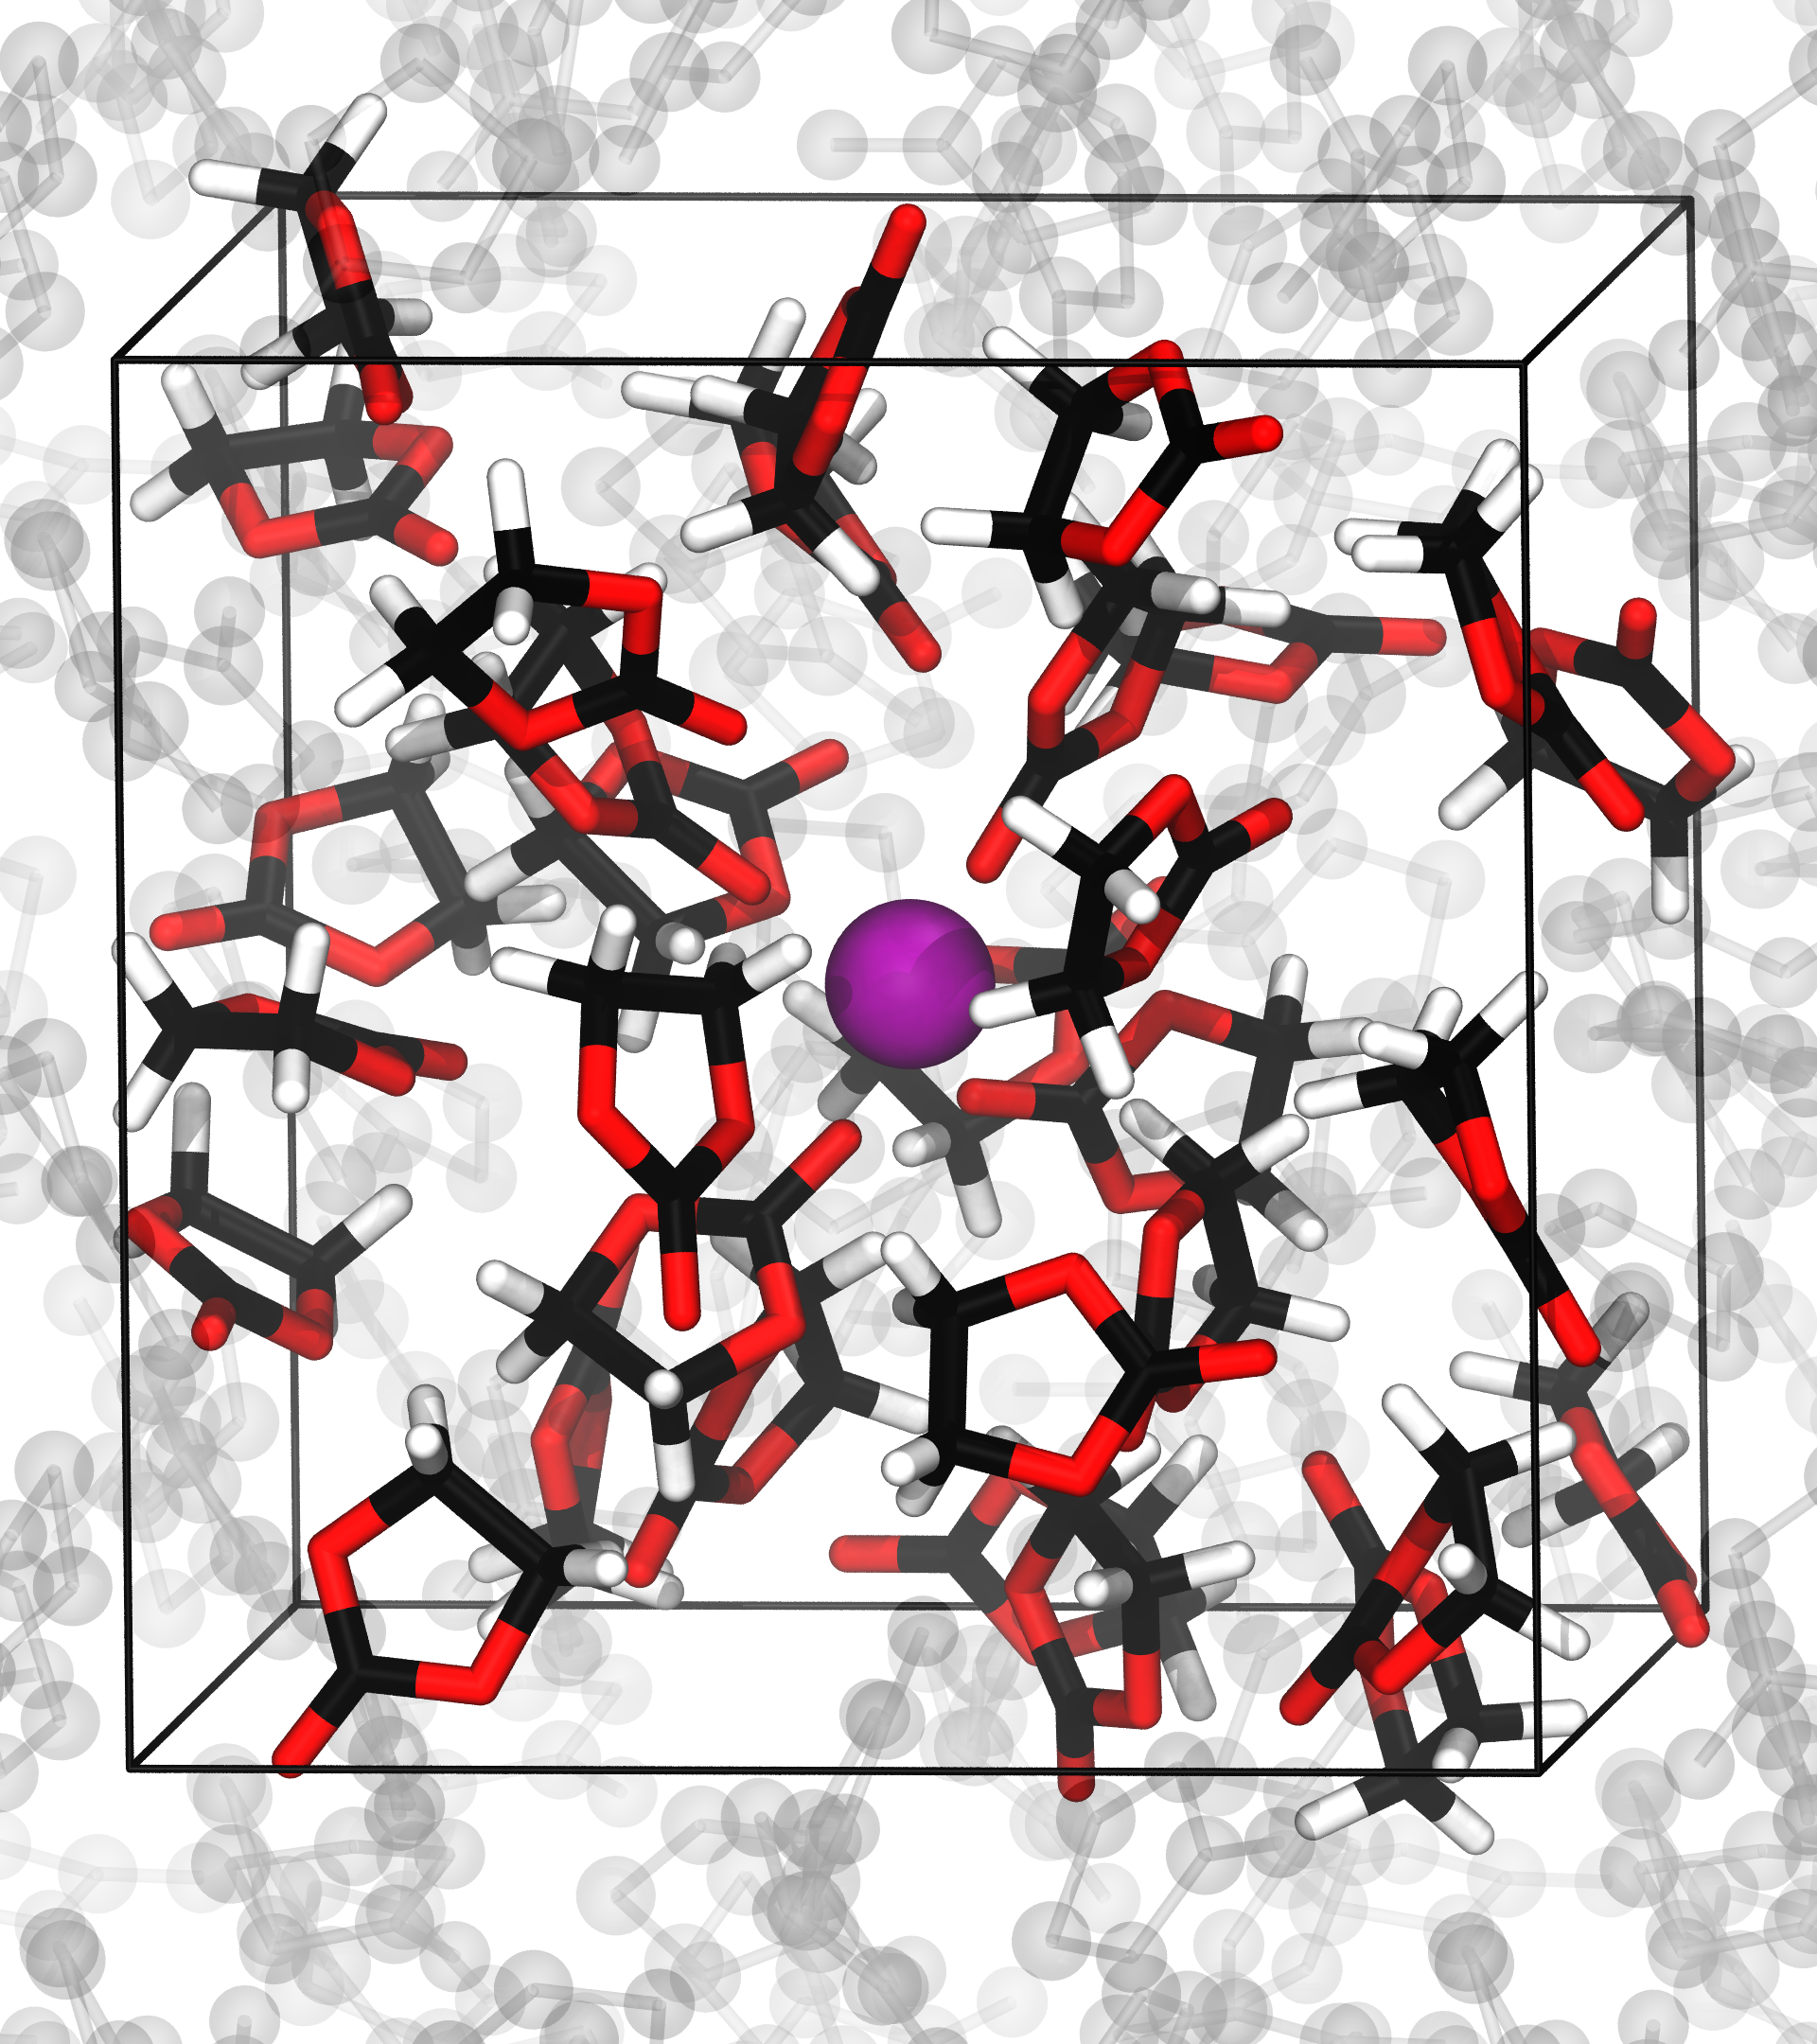
\includegraphics[width=0.98\linewidth]{images/ecpc/toc_liec_default.png}
 \caption[Snapshot of (Li\sur{+}EC\sous{31})]{\label{fig:liec_snap}Snapshot of (Li\sur{+}EC\sous{31}).}
\end{figure}

   \subsection{\label{ch4:sec1:level4}DFT-D3 symmetry adapted perturbation theory}
    Clusters of the nearest 4 molecules centered around the Li\sur{+} ion were extracted from both classical and density functional based trajectories
    of the slightly larger Li\sur{+}EC\sous{31} and Li\sur{+}PC\sous{31} systems. These coordinates were then used as inputs for a symmetry adapted 
    perturbation theory (SAPT) decomposition of the ion/solvent interaction energies at the SAPT(KS)-D3 level. D3 refers to the 3\sur{rd} generation
    dispersion potential of Herbert et al.\cite{lao2014xsaptksd3}. We picked 600 configurations initially, excluding only 2 outliers from the Li\sur{+}EC\sous{31} DFT-generated 
    trajectory and 8 each from the Li\sur{+}PC\sous{31} trajectories for which had produced nonsensical results. We have chosen to retain the the PBE 
    functional in this analysis but slightly increased the accuracy of the basis set to jun-cc-pVDZ and resolution of the identity (RI) approximation 
    optimized jun-cc-pVDZ-RI. Li\sur{+} uses the cc-pVDZ equivalent in both of these basis sets. Benchmarking shows SAPT(KS)-D3 and the related XSAPT 
    method performance is significantly enhanced through the introduction of diffuse functions. The version of SAPT(KS) implemented in QChem 4.4\cite{krylov2013qchem,shao2006qchem} takes 
    advantage of a long-range correction added to the Coulomb potential at a range controlled via a splitting parameter, $\omega$. We optimized the 
    parameters as reported by Herbert et al. with the above basis sets and method\cite{lao2014xsaptksd3}. A value of 8000 bohr\sur{-1} was required for Li\sur{+}, 540 
    bohr\sur{-1} for EC, and 365 bohr\sur{-1} for PC.
  
  \section{\label{ch4:sec2:level1}Results}
   Table \ref{tab:dipoles} lists the average dipole moment of the carbonate molecules from the gas and condensed phase simulations. Error bars were
   calculated with the block-averaging method. A single standard deviation is also included to assess the spread of width the distribution of dipoles.
   Gas phase dipoles for EC exhibited small fluctuations about a mean of 5.44 D. The change from H to CH\sous{3} in PC produced a small increase in 
   the average dipole moment to 5.65 D. In the condensed phase, these dipoles rose by 34\% each! The bulk EC value averaged to 7.30 D and the PC value
   to 7.56 D. Each of these solvents exhibited fluctuations in excess of 0.5 D with EC producing slightly larger fluctuations, possibly owing to the
   more mobile H group and potential steric clashes with neighboring molecules due to the larger CH\sous{3} group. 
   
   Basis set dependence of these quantities is also examined and I found virtually no change in the condensed phase dipoles. There was some 
   fluctuation in the gas phase dipoles just beyond my error estimate, but these settle back down to those predicted by the smallest basis
   set (which I used to generate the trajectories) for the largest basis considered.

\begin{table}
 \begin{center} 
  \begin{tabular}{cccc}
   \hline
   \hline
    System          & $\left<\mu\right>$ & $\sigma$ & $\left<\mu\sous{blk}\right>$/$\left<\mu\sous{gp}\right>$ \\
   \hline
    \\ 
    \multicolumn{4}{c}{\textbf{DZVP-MOLOPT-SR-GTH}} \\ 
    \\
    EC\sous{1,gp}   & 5.44 $\pm$ 0.05   & 0.28 &      \\
    EC\sous{32,blk} & 7.30 $\pm$ 0.22   & 0.55 & 1.34 \\
    PC\sous{1,gp}   & 5.65 $\pm$ 0.07   & 0.29 &      \\
    PC\sous{32,blk} & 7.56 $\pm$ 0.24   & 0.52 & 1.34 \\
    \\ 
    \multicolumn{4}{c}{\textbf{DZVP-MOLOPT-GTH}} \\ 
    \\
    EC\sous{1,gp}   & 5.51 $\pm$ 0.05   & 0.29 &      \\
    EC\sous{32,blk} & 7.30 $\pm$ 0.11   & 0.56 & 1.32 \\
    PC\sous{1,gp}   & 5.71 $\pm$ 0.06   & 0.30 &      \\
    PC\sous{32,blk} & 7.55 $\pm$ 0.14   & 0.53 & 1.32 \\
    \\ 
    \multicolumn{4}{c}{\textbf{TZVP-MOLOPT-GTH}} \\ 
    \\
    EC\sous{1,gp}   & 5.50 $\pm$ 0.05   & 0.29 &      \\
    EC\sous{32,blk} & 7.34 $\pm$ 0.11   & 0.57 & 1.33 \\
    PC\sous{1,gp}   & 5.70 $\pm$ 0.06   & 0.30 &      \\
    PC\sous{32,blk} & 7.59 $\pm$ 0.15   & 0.54 & 1.33 \\
    \\ 
    \multicolumn{4}{c}{\textbf{TZV2P-MOLOPT-GTH}} \\ 
    \\
    EC\sous{1,gp}   & 5.48 $\pm$ 0.05   & 0.29 &      \\
    EC\sous{32,blk} & 7.33 $\pm$ 0.11   & 0.57 & 1.34 \\
    PC\sous{1,gp}   & 5.67 $\pm$ 0.06   & 0.30 &      \\
    PC\sous{32,blk} & 7.58 $\pm$ 0.15   & 0.54 & 1.34 \\
    \\     
    \multicolumn{4}{c}{\textbf{TZV2PX-MOLOPT-GTH}} \\ 
    \\
    EC\sous{1,gp}   & 5.47 $\pm$ 0.05   & 0.29 &      \\
    EC\sous{32,blk} & 7.34 $\pm$ 0.09   & 0.56 & 1.34 \\
    PC\sous{1,gp}   & 5.66 $\pm$ 0.06   & 0.30 &      \\
    PC\sous{32,blk} & 7.58 $\pm$ 0.17   & 0.54 & 1.34 \\    
   \hline
   \hline
  \end{tabular}
  \caption[Gas and condensed phase dipole moments with varying basis set]{\label{tab:dipoles}Dipole moments (in Debye) $\pm$ 
  standard error in the mean using the block averaging method.
  A single sample standard deviation is provided to get a sense of the distribution of molecular dipoles about the mean. 
  The third column is the ratio of the bulk dipole moment to the gas phase measurement.}
 \end{center}
\end{table}

   Solvation structure around the Li\sur{+} ion is shown in Figure \ref{fig:rdf}. Both solvents give peaks in the radial distribution function at a distance of 200 pm.
   The coordination number resulting from integration to the first minimum is about 4 for each solvent. The actual values at the minima are 3.88 at 287.5 pm for EC and 
   3.98 at 277.5 pm for PC. The cutoff is very clean for PC and less so for EC where the g(r) smoothly increases through to the second, much broader shell which peaks 
   in both solvents just shy of 800 pm.

\begin{figure}
 \begin{center}
 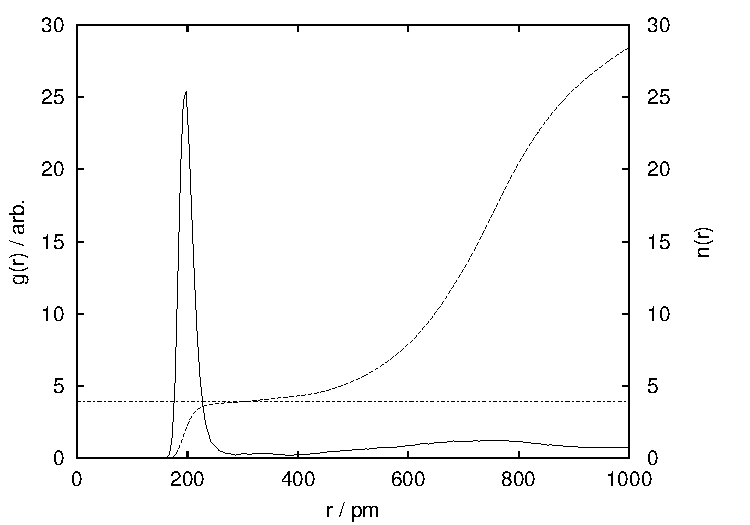
\includegraphics[width=0.8\linewidth]{images/ecpc/liec_32-noWC-rdf.pdf} \\
 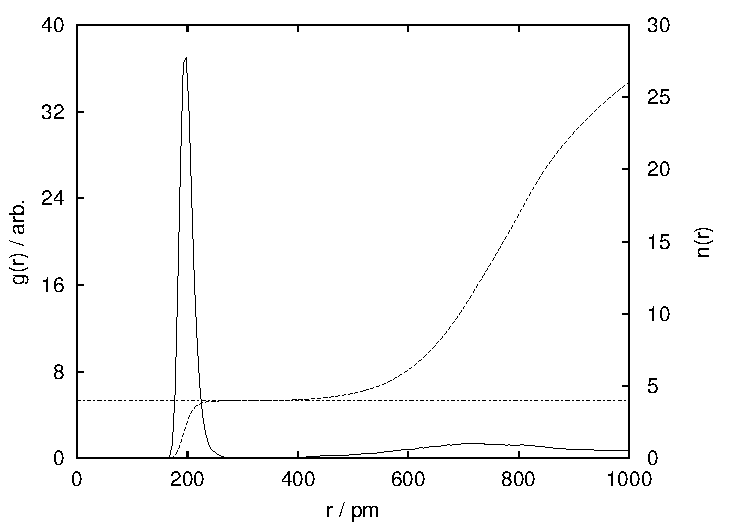
\includegraphics[width=0.8\linewidth]{images/ecpc/lipc_32-noWC-rdf.pdf}
 \end{center}
 \caption[Li$^{+}$ and carbonyl oxygen radial distribution functions]{\label{fig:rdf}Li\sur{+} and carbonyl oxygen radial distribution 
 functions for ethylene carbonate (top) and
 propylene carbonate (bottom). The distribution function is depicted with a solid line while the number integral is 
 shown as a dashed line. A dashed horizontal line passes provides an estimate of the coordination number in the first
 solvation shell which are both very close to n $=$ 4.}
\end{figure}

   The distribution of dipole moments of EC and PC molecules as a function of distance from the Li\sur{+} are shown in Figures \ref{fig:ec_cdf} and \ref{fig:pc_cdf}. 
   Horizontal lines in these plots point out the gas phase and condensed phase averages from above (from the DZVP-MOLOPT-SR-GTH data). These dipoles are also computed 
   with the short range basis. The x-axis reflects the distance between the ion and carbonyl oxygen. The density distribution of the EC molecules maxes near the ion
   at a dipole moment of $\sim$8.4--8.5 D and in PC at $\sim$8.7--8.8 D. Each of these figures is slightly greater than 50\% larger than those measured in the gas 
   phase and approaching 20\% larger than those measured in neat solutions. The wide spread of the dipole moments in the first shell is indicative of the fairly 
   labile nature of the solvation shell for EC especially. There's definitely more accumulation between the first and second solvation shells for this system which
   corresponds to the solvent in reverse orientation with the carbonyl directed away from the ion. This appeared to occur less frequently in PC, probably because 
   PC is modeled at a lower temperature.

\begin{figure}
 \begin{center}
 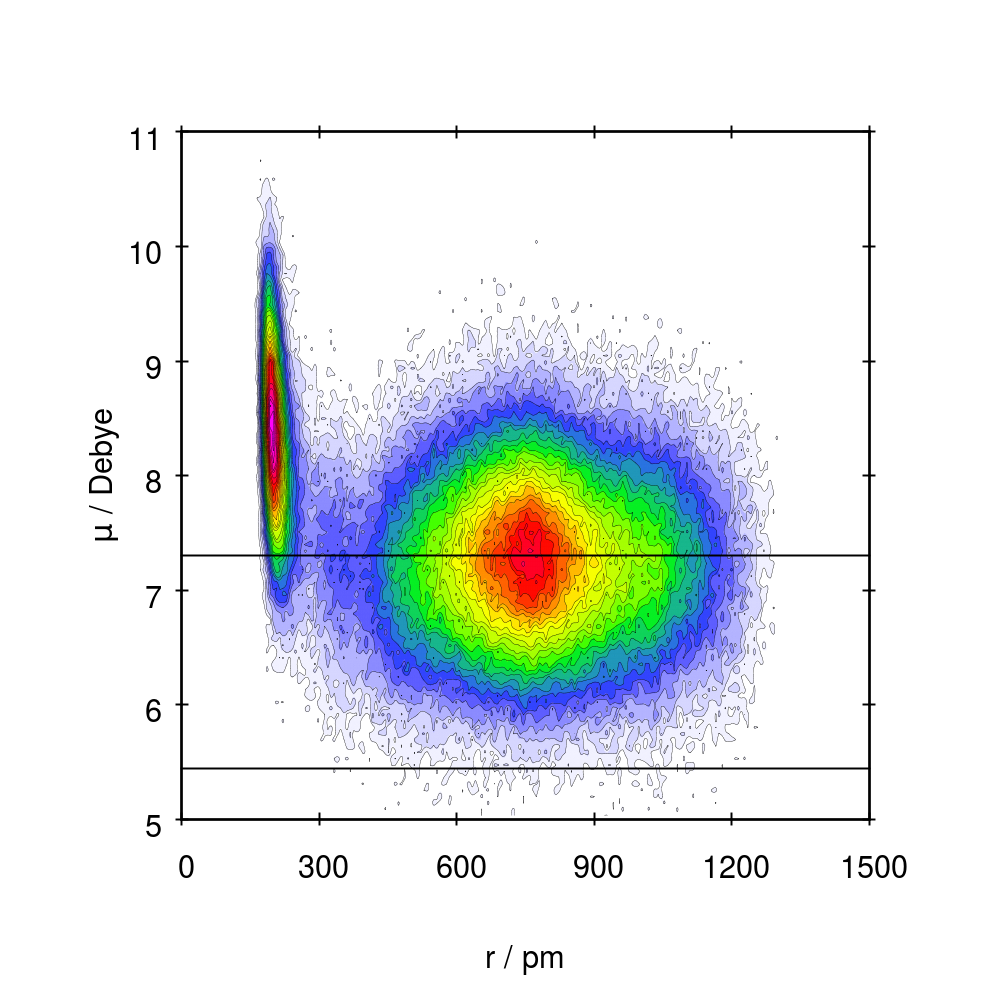
\includegraphics[width=0.98\linewidth]{images/ecpc/cdf_2_rdf_dipoleC3H4O3.png} \\
 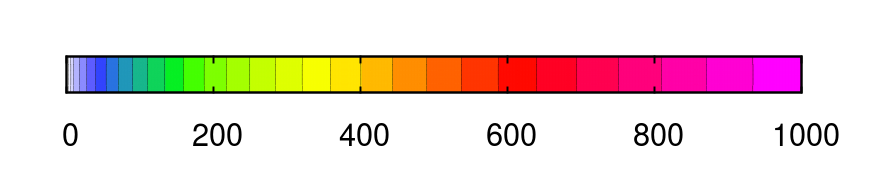
\includegraphics[width=0.5\linewidth]{images/ecpc/cdf_2_rdf_dipoleC3H4O3_box.png}
 \end{center} 
 \caption[Ethylene carbonate dipoles versus distance from ion]{\label{fig:ec_cdf}Combined density distribution of ethylene 
 carbonate dipole moment as a function of radial
 distance from the ion. Colors map to raw counts delineated in the color bar. Solid, horizontal lines highlight average
 gas and condensed phase dipole moments from Table \ref{tab:dipoles}. Images aren't centered because I will be adding an 
 image to the upper right corner.}
\end{figure}

\begin{figure}
 \begin{center}
 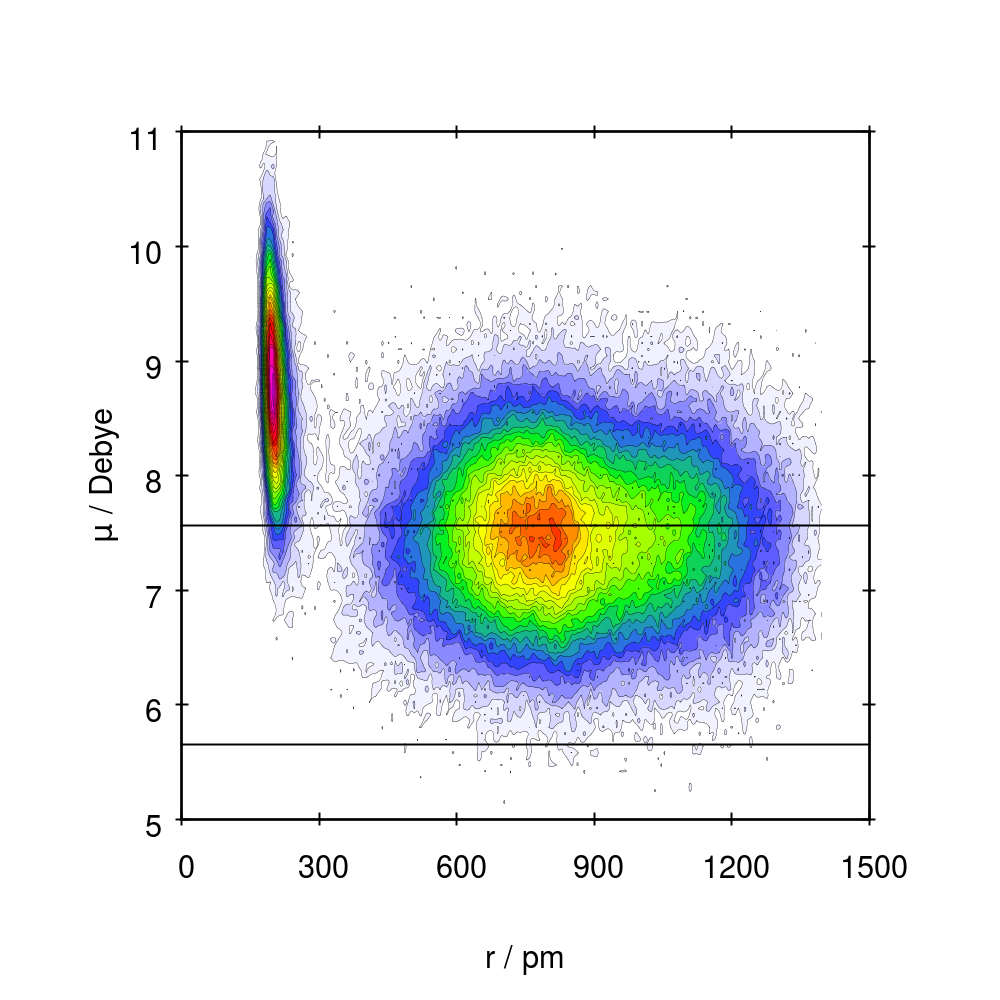
\includegraphics[width=0.98\linewidth]{images/ecpc/cdf_2_rdf_dipoleC4H6O3.png} \\
 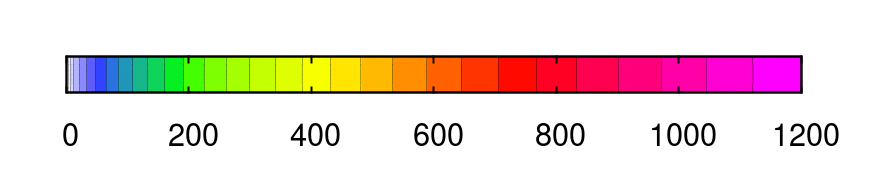
\includegraphics[width=0.5\linewidth]{images/ecpc/cdf_2_rdf_dipoleC4H6O3_box.png}
 \end{center} 
 \caption[Propylene carbonate dipoles versus distance from ion]{\label{fig:pc_cdf}Combined density distribution of propylene
 carbonate dipole moment as a function of radial
 distance from the ion. Colors map to raw counts delineated in the color bar. Solid, horizontal lines highlight average
 gas and condensed phase dipole moments from Table \ref{tab:dipoles}. Image not centered, same reason.}
\end{figure}

   SAPT(KS)-D3 results are shown in Figures \ref{fig:ecsapt1} through \ref{fig:pcsaptint}. The more rigid nature of the classical force field universally produced
   less broad distributions in the energy terms than the density-functional configurations. The greater bond length between the ion and solvent in the GAFF model
   likewise produced smaller attractive energies, though the disparity is greater for PC configurations than EC. This also produced less overlap between the atoms
   and so gave smaller exchange and exchange-coupled energy contributions. For EC, the greatest differences were reflected in the induction energies. In PC, both
   1\sur{st} and 2\sur{nd} order energy contributions failed to overlap significantly. In the total intermolecular energies (which include dispersion and the infinite
   order corrections), there is greater overlap between the classical and \emph{ab initio} models with EC and very little for PC. These data suggest that the force 
   field relies on error cancellation (the smaller exchange energies) to make up for their underestimation of attractive components due to the longer bond lengths.

  \section{\label{ch4:sec3:level1}Discussion}
   The dipole moments I report are a fair bit larger than those often used in literature. For pure EC and PC, 4.61 D and 4.81 D are most often cited\cite{ayse2016ecpc,peruzzi2015solvation}.
   These are each about 85\% of the values reported in Table \ref{tab:dipoles}. However, the larger dipole moments found here match those from the theoretical predictions of Hammer et 
   al.\cite{hammer2004dipole}, Luber\cite{luber2014local} (including the condensed phase $\left<\mu\right>$ and standard deviation for EC), Masia et al.\cite{masia2004ethylene}, Park et 
   al.\cite{park2011low}, Stark-effect measurements by Alonso et al.\cite{alonso1986microwave}, and back-calculating the dipole from capacitance measurements by Chernyak\cite{chernyak2006dielectric}. 
   Only the works of Park et al. and Chernyak made an attempt at the dipole moment of PC. Chernyak's estimate of the EC dipole is 4.81 D but 5.36 D for PC, closer to the result I 
   obtained\cite{chernyak2006dielectric}.
   
   Interaction energies are an interesting story as well. Averages taken of my data in Figures \ref{fig:ecsaptint} and \ref{fig:pcsaptint} are nearly identical, though the EC distribution
   is obviously a fair bit broader than the PC one. This reflects the increased frequency of structures where one of the solvent molecules is being exchanged with the bulk and is often
   nearly completely turned around. This is seen in Figures \ref{fig:ec_cdf} and \ref{fig:pc_cdf} as the increased density of ion-carbonyl oxygen distances around 300 pm. Given that an
   increased temperature in the Li\sur{+}/PC simulations would serve to broaden the interaction energy distribution and that the largest binding energies were observed for Li\sur{+}/EC 
   despite the greater thermal stresses, it is reasonable to conclude that the binding energy between Li\sur{+}/EC is greater than Li\sur{+}/PC, consistent with some of the experiments 
   discussed in Chapter \ref{ch1:sec5:level1}. However, Peruzzi et al. found the solvation enthalpies of KX salts were more favorable in PC than EC. The binding energies of Park et al.
   support this conclusion as well\cite{park2011low}, as does the SAPT work by Arslanargin et al.\cite{ayse2016ecpc}. There's a split in the thermodynamic data of anions at Cl\sur{-}
   which was determined to be better solvated in EC than PC. The similar solvent reorganization energies in this study suggest that the differences lie primarily in the strength of 
   ion/solvent interactions. My SAPT energies using classically generated coordinates favor Li\sur{+}/EC over Li\sur{+}/PC while K\sur{+} was found to be better solvated in PC\cite{ayse2016ecpc}. 
   There may be a cutoff here as well, similar to that in water. Clearly, there is no consensus on relative binding energies of ions with the cyclic carbonates.
   
   Radial distribution functions and the coordination number have been another point of contention in the literature. As reviewed earlier in Chapter \ref{ch1:sec5:level1}, the 
   coordination number is typically taken to be somewhere in the range of 4--5, though it has been determined to be as high as $\sim$7\cite{castriota2003temperature}. The integral
   taken to the minimum of the first peak of my radial distribution functions in Figures \ref{fig:rdf} is $\sim$4 in each solvent. Again, the actual values were found to be 3.88 for EC 
   and 3.98 for PC. These values are identical to those from other theoretical studies but smaller than most of the experimental measurements discussed previously. Since the methodology
   I used was based off of the work of Leung et al.\cite{leung2010liion}, it's excellent to see that our g(r) have very similar profiles. Both g(r)'s peak at 200 pm for the Li\sur{+}-O(carbonyl) distance
   and have an intensity of just over 25. Distributions taken from Arslanargin et al.\cite{ayse2016ecpc} and Masia et al.\cite{masia2004ethylene} show over-structuring of the first 
   solvation shell, each with intensities over 40. The location of the maximum in each of these distributions also differs from both mine and Leung's. The classical models tend to give
   too small an average bond length between Li\sur{+} and EC, though one of the results from Arslanargin et al.\cite{ayse2016ecpc} gives too great a distance (and a coordination number
   of 6). This model is identical to the one used in this study to prepare the initial coordinates for AIMD work. For PC, the location of the first peak was found by Smith et al.\cite{smith2014x} 
   to also be around 200 pm, though their simulated model is less structured than mine with an intensity similar to that of my Li\sur{+}/EC result. This may simply reflect temperature 
   differences.

  \section{\label{ch4:sec4:level1}Conclusions $\&$ Future Work}
   Up to this point, I have determined that polarizability is an important consideration in the condensed phase behavior of cyclic carbonates ethylene carbonate and propylene carbonate.
   The dipole moments which were found to be 5.44 D and 5.65 D in the gas phase increase by $\sim$34\% through self-polarization in the condensed phase to 7.30 D and 7.56 for EC and PC,
   respectively. This increase may be approximately handled in classical models which appear to reproduce the dielectric constant of the pure solvents over a broad temperature range\cite{you2015dielectric}.
   However, when attempting to address problems of ion solvation, the dipole moments of these solvents increase even further by about 50\% over the gas phase dipole moments to about
   $\sim$8.4--8.5 D and in PC at $\sim$8.7--8.8 D in the first solvation shell around Li\sur{+}. While in water there is some evidence to suggest that the dipole moments of waters
   coordinated to the ions more or less return to the bulk value or produce modest increases ($<$10\%)\cite{heuft2003cl,heuft2005f,heuft2005i,krekeler2006density,lightstone2001first}, it is clear from my results that this may not be the case 
   in solvents with larger polarizabilities. Interaction energies suggested better solvation of Li\sur{+} in EC than in PC, though the extent to which EC is favored cannot be predicted
   from these results. The coordination structure of EC and PC around Li\sur{+} compared well against other simulation results and the coordination numbers were found to be very close 
   to 4 in each of the solvents, consistent with other theoretical calculations. These fall short of the assumed values from experimental measurements which tend closer to 5 EC or PC
   per Li\sur{+}.
   
   Before publishing this work I have several other pieces of data to add and I may collaborate with Matthew Brown to calculate X-ray absorption spectra to predict Li\sur{+}-1s binding
   energies. The binding energy of the core state was shown by Matt Brown to be a probe of the strength of ion/solvent interactions\cite{brown2015ion}. By comparing the binding energy
   in a fictitious state where the gas phase optimized EC and PC molecules are superimposed on the positions of solvent molecules in Li\sur{+}/XC\sous{4} clusters (X = E and P) versus 
   the binding energy of the Li-core state in the fully interacting cluster, I hope to approximately determine the effect of polarization. Alternative approaches will likely be 
   considered as well. Another possibility is to perform a many-body expansion where a distinguished EC or PC interaction energy is measured with Li\sur{+} left out.
   I am also going to add data for PC simulated at 450 K as well. The choice of 350 K was motivated to mimic the temperature increase in EC over its melting point 
   to simulate a liquid phase just above each solvent's freezing temperature. It is clear that a 450 K simulation of PC would prove useful in addressing some other concerns about the
   binding energy and X-ray spectra by eliminating the thermal differences. The additional data includes sampling the dipole moments from the simulations using the GAFF model, calculating 
   interaction energies for small clusters using the GAFF interaction potential, and measuring EC and PC structural properties of molecules in the first shell and relating them to their
   dipole moment (to address how the structure changes to produce the larger dipole moment).
  
\end{ecpc}
 % ec/pc paper
 \begin{cpa}
 \chapter{Thermodynamics of proton hydration and the electrochemical surface potential}
 \hyperlink{toc}{Return to TOC}
  \section{\label{ch5:sec0:level1}Preface}
  Much of the text presented here has been adapted from the following publications,
  
  \vspace{12pt}
  \noindent \emph{Travis P.~Pollard, Thomas L.~Beck, Quasichemical analysis of the cluster-pair approximation for the thermodynamics of proton hydration, 
  J. Chem. Phys. \textbf{140} (22) 2014.}

  \noindent \emph{Travis P.~Pollard, Thomas L.~Beck, The thermodynamics of proton hydration and the electrochemical surface potential of water, J. Chem. Phys. 
  \textbf{141} (18C512) 2014.}
  \vspace{12pt}
  
  These articles summarize the findings of my computational analysis of the cluster-pair approximation (CPA) for the determination of single-ion free energies and
  enthalpies from the extrapolation of cluster data to the bulk. The CPA expression of these quantities for the proton includes an interfacial potential 
  contribution by definition. It is shown, however, that the CPA involves an extra-thermodynamic assumption that does not guarantee uniform convergence to a bulk 
  free energy or enthalpy value with increasing cluster size. I use computational modeling to examine the size-dependence of the differences in the hydration enthalpies 
  for the Na\sur{+}/F\sur{-} ion pair in water clusters of size \emph{n} = 1, 2, 3, \dots, 200 (not perfectly sequential, there are some breaks). A sizable shift from
  the accepted cluster-pair approximation value is found for the proton hydration enthalpy for cluster sizes just beyond the limits used in the CPA. The shifts arise 
  from a combination of sequential hydration and interfacial potential effects and converges at large \emph{n} to a value of -0.4 V to -0.5 V depending on the
  temperature derivative of the interfacial potential being used. The -0.4 V result is argued to be preferable and assumes the temperature derivative to be close to
  0.~cal/mol-K-\emph{e}. In response to concerns raised that the 2$^{nd}$ order M$\text{\o}$ller-Plesset (MP2) energy overestimates the dispersion energy in 
  F\sur{-}/water clusters leading to the shift\cite{herbert2014personal}, I have included previously unpublished evaluations of the enthalpy differences using the 
  `gold standard' CCSD(T) method. Though the cluster size is severely limited, the beginnings of the shift are shown to be preserved.
  
  This section addresses three of the questions I posed in Chapter \ref{ch1:sec1:level4},
   
   \begin{itemize}
       \item Do chemical interfaces contribute to single-ion thermodynamics? 
       \item If so, what is the contribution?
       \item How can we compare our simulation results to experiment?
   \end{itemize}
  
  \section{\label{ch5:sec1:level1}The cluster pair approximation}
  The cluster-pair approximation\cite{coe1998cpa1} (CPA) is widely viewed as the most accurate approach for determining the hydration free energy of the 
  proton\cite{camaioni2005stdstcorr,kelly2006cpa} Given the hydration free energy of one ion, all other single-ion free energies can be obtained from bulk 
  thermodynamic data\cite{conway1978evaluation,marcus1985book}. The CPA approach utilizes ion-water cluster data and bulk conventional ion hydration free energies 
  (referenced to the proton), along with an insightful analysis, to infer the proton hydration enthalpy and free energy. Recently, the issue has been
  raised as to whether the CPA may involve an extra-thermodynamic assumption that could result in proton values that deviate from those predicted based
  on small-cluster data\cite{donald2010expand_cpa,hunenberger2011sp,vlcek2013cpa,vlcek2016cpareview}. This deviation is predicted to result from two
  parts: 1) hydration effects and 2) the net potential of water $\phi\sous{np}$. At large \emph{n} it is expected that the shift be comprised of 
  $\phi\sous{np}$ alone.

  The excess chemical potential can be written as\cite{aquaincognita2014} 
  
  \begin{equation} 
    \mu_X^{ex} = \mu_{X,b}^{ex} + q\phi_{np}
    \label{eq:echemmu}
  \end{equation}

  \noindent where $\mu_{X,b}^{ex}$ is the bulk hydration free energy (that includes all interactions of the ion with water except for the net potential 
  contribution), see discussion in Chapter \ref{ch1:sec4:level1}. $\mu_{X,b}^{ex}$ is also called the \emph{intrinsic} free energy\cite{hunenberger2011sp}
  and $\mu_X^{ex}$ the \emph{real} free energy. Similar nomenclature is extended to the hydration enthalpy which is
  
  \begin{equation}
    h_X^{ex} = h_{X,b}^{ex} + q\phi_{np} - qT\left(\frac{\partial \phi_{np}}{\partial T}\right)_P
    \label{eq:echemh}
  \end{equation}

  \noindent and the hydration entropy\cite{lynden1997hydrophobic} is

  \begin{equation}
    s_X^{ex} = s_{X,b}^{ex} - q\left(\frac{\partial \phi_{np}}{\partial T}\right)_P.
    \label{eq:echems}
  \end{equation}

  \noindent In these papers, standard states of 1 M concentration in both the vapor and liquid phases are used so that the free energies and entropies 
  reflect excess quantities that do not include superfluous volume changes. The experimental value for the temperature derivative is taken as -9.9 
  cal/mol-K-\emph{e}\cite{randles1977structure}, though there is evidence this value is much too negative\cite{donald2010expand_cpa,vlcek2013cpa}.

  To understand the origins of the CPA, consider the exact QCT expression for the ion excess chemical potential from Ref. \cite{asthagiri2010ion}
  
  \begin{equation}
    \mu_X^{ex} = -kT \ln [K_{X,n}^{(0)} \rho_W^n] + kT \ln p_X(n) + \mu^{ex}_{XW_n} - n\mu^{ex}_W  
    \label{eq:qctcpl}
  \end{equation}

  \noindent where $K_{X,n}^{(0)}$ is the equilibrium constant for the formation of the $XW_n$ cluster in the gas phase, $\rho_W$ is the bulk density of 
  water, $p_X(n)$ is the probability of observing \emph{n} waters complexed with the ion in bulk water, $\mu^{ex}_{XW_n}$ is the free energy to insert the 
  cluster into bulk water, and $\mu^{ex}_W$ is the free energy to insert one water molecule into bulk water.

  Collecting all terms but the free energy to hydrate the cluster into a single term $\mu^{ex}_{X,n}$
  
  \begin{equation}
    \mu_X^{ex} =  \mu^{ex}_{X,n} + \mu^{ex}_{XW_n}  
    \label{eq:qctcpa}
  \end{equation}

  \noindent where
  
  \begin{equation}
    \mu^{ex}_{X,n} = -kT \ln K_{X,n}^{(0)} + kT \ln p_X(n) - n \left[ kT \ln \rho_W  + \mu^{ex}_W \right] 
    \label{eq:qctcpaxn}
  \end{equation}

  \noindent The first two terms on the right side of Eq. \ref{eq:qctcpaxn} are ion specific, while the last term involves properties of bulk water.
  The cluster experimental data employed in the CPA\cite{coe1998cpa1} involves the temperature dependence of $K_{X,n}^{(0)}$ for small clusters 
  \emph{n} = 1--6. The CPA relies on differences of free energy and enthalpy terms for positive/negative ion pairs. Then all terms in $\mu^{ex}_{X,n}$ 
  except $K_{X,n}^{(0)}$ cancel when taking the differences (for large \emph{n}, the term involving $p(n)$ should also cancel nearly exactly).

  The terms in Eq. \ref{eq:qctcpa} correspond to a 2-step process for analyzing the hydration free energy: formation of the ion-water cluster 
  followed by insertion of the cluster into bulk water. It is clear on physical grounds that cation/anion differences of $\mu^{ex}_{XW_n}$
  approach zero as the cluster size approaches infinity, since this is the free energy to insert a large ion/water cluster into bulk water, and on
  average the ion is thus shielded from the surrounding bulk water. 

  The input data for the CPA\cite{coe1998cpa1} includes differences of bulk conventional free energies and cluster formation free energies for cation/anion 
  pairs; the cluster free energies are available for a range of ions with \emph{n} = 1--6 clustered waters. These data have been assembled from mass 
  spectrometric analyses on ion/water clusters with size discrimination based on collision energy\cite{wheeler2015hydration} or other means and theoretical 
  calculations\cite{coe1998cpa1,coe2001cpa2,coe2002cpa3,donald2010expand_cpa,kelly2006cpa}.
  
  The bulk conventional free energies are defined as
  
  \begin{equation}
    \mu_N^{ex,con} =  \mu^{ex}_{N} + \mu^{ex}_{\mathrm{H}^+} = \mu^{ex}_{N,b} + \mu^{ex}_{\mathrm{H}^+,b}
    \label{eq:con1}
  \end{equation}

  \noindent for a negatively charged ion and

  \begin{equation}
    \mu_P^{ex,con} =  \mu^{ex}_{P} - \mu^{ex}_{\mathrm{H}^+} = \mu^{ex}_{P,b} - \mu^{ex}_{\mathrm{H}^+,b}
    \label{eq:con2}
  \end{equation}
  
  \noindent for a positively charged one, where the bulk free energies are $\mu^{ex}_{X,b} = \mu^{ex}_{X} - q\phi_{np}$. The conventional free 
  energies can be obtained from bulk thermodynamic data, and it is apparent that the net potential does not appear explicitly in Eqns. \ref{eq:con1} 
  and \ref{eq:con2} due to the cancellation between the ion and proton terms. The conventional free energy scale is set relative to the proton,
  just as the electrochemical scale (the standard hydrogen electrode has a potential of 0. V, when the \emph{real} potential is estimated at 
  -4.44 $\pm$ 0.02 V\cite{trasatti1986absolute}).

  The CPA is an analysis method that leads to an estimation of the proton hydration free energy, enthalpy, and entropy. For brevity, I'll review
  only the free energy `path.' First, consider the free energy difference between a cation ($P$) and anion ($N$), defined for example as
  
  \begin{equation}
    \Delta \mu_X^{ex,con} =  \mu^{ex,con}_{N} - \mu^{ex,con}_{P}  
    \label{eq:cpadiff}
  \end{equation}

  \noindent so the change refers to the $P \rightarrow N$ transition for a given ion pair. Combining this expression with those above in Eqns.
  \ref{eq:con1} and \ref{eq:con2} results in the following relationships

  \begin{equation}
    \frac{1}{2} \Delta \mu_{X}^{ex,con} - \frac{1}{2} \Delta \mu_{X}^{ex} = \mu^{ex}_{\mathrm{H}^+}
    \label{eq:cpa1}
  \end{equation}

  \noindent and
  
  \begin{equation}
    \frac{1}{2} \Delta \mu_{XW_n}^{ex,con} -  \frac{1}{2} \Delta \mu_{XW_n}^{ex} = \mu^{ex}_{\mathrm{H}^+}.
    \label{eq:cpa2}
  \end{equation}

  \noindent It is also true that 
  
  \begin{equation}
    \frac{1}{2} \Delta \mu_{X}^{ex,con} - \frac{1}{2} \Delta \mu_{X,b}^{ex} + \phi_{np} = \mu^{ex}_{\mathrm{H}^+}
    \label{eq:cpa1bulk-1}
  \end{equation}
  
  \noindent and 

  \begin{equation}
    \frac{1}{2} \Delta \mu_{X}^{ex,con} - \frac{1}{2} \Delta \mu_{X,b}^{ex} = \mu^{ex}_{\mathrm{H}^+,b}.
    \label{eq:cpa1bulk}
  \end{equation}

  \noindent Since $\Delta \mu_{X}^{ex}$ and $\Delta \mu_{XW_n}^{ex}$ are not available from experiment, the CPA makes an assumption to deal with 
  these terms. 

  $\Delta \mu_{X}^{ex,con}/2$ contains no explicit net potential contribution; it is clear from Eq. \ref{eq:qctcpa}, however, that $\Delta 
  \mu_{XW_n}^{ex,con}/2$ can develop an explicit net potential contribution for large \emph{n} due to the cluster term (since $\Delta 
  \mu^{ex,con}_{X} = \Delta \mu^{ex}_{X,n} + \Delta\mu^{ex,con}_{XW_n}$). It is also clear from Eq. \ref{eq:cpa2} that, in the limit of large 
  \emph{n}, $\Delta \mu_{XW_n}^{ex,con}/2 = \mu^{ex}_{\mathrm{H}^+}$.

  Eq. \ref{eq:cpa1} can be rewritten as
  
  \begin{equation}
    \frac{1}{2} \Delta \mu_{X}^{ex,con} - \frac{1}{2} \left[ \mu_{N,n}^{ex}/c_{N,n} - \mu_{P,n}^{ex}/c_{P,n} \right] = \mu^{ex}_{\mathrm{H}^+}
    \label{eq:cpa3}
  \end{equation}
  
  \noindent where $c_{N,n} = \mu_{N,n}^{ex}/\mu_{N}^{ex}$ and $c_{P,n} = \mu_{P,n}^{ex}/\mu_{P}^{ex}$. The central assumption of the 
  CPA\cite{coe1998cpa1} is then to create a composite term for the chosen $N/P$ pair:

  \begin{equation}
    \bar{c}_{X,n} = \frac{\mu_{N,n}^{ex} + \mu_{P,n}^{ex}}{\mu_{N}^{ex} + \mu_{P}^{ex}}
    \label{eq:cpacomp}
  \end{equation}
  
  \noindent where now the quantities are experimentally available. Then

  \begin{equation}
    \frac{1}{2} \Delta \mu_{X}^{ex,con} - \frac{1}{2\bar{c}_{X,n}} \Delta \mu_{X,n}^{ex} \approx \mu^{ex}_{\mathrm{H}^+}
    \label{eq:cpafinal}
  \end{equation}
  
  \noindent Since the exact relation involves 
  
  \begin{equation} 
    \bar{c}_{X,n} (\mathrm{exact}) = \frac{\mu_{N,n}^{ex} - \mu_{P,n}^{ex}}{\mu_{N}^{ex} - \mu_{P}^{ex}} = \frac{\Delta \mu^{ex}_{X,n}}{\Delta \mu^{ex}_{X}}
    \label{eq:cpacompex}
  \end{equation}

  \noindent it is seen that the CPA involves an extra-thermodynamic assumption. In plain language, the assumption is that the differences
  in the pair solvation free energies for the small clusters should converge rapidly to the bulk limit and remain roughly constant to
  large \emph{n}. As mentioned previously, this is not necessarily the case\cite{donald2010expand_cpa,vlcek2013cpa,vlcek2016cpareview}.
 
  Assembling many differences for the alkali/halides and even broader ion sets, the results can be plotted as in Kelly, Cramer, and 
  Truhlar\cite{kelly2006cpa} (Figure 1 of Ref. \cite{kelly2006cpa}). The $y$ axis is 
  
  \begin{equation}
    y(n)=\frac{1}{2} \Delta \mu_{XW_n}^{ex,con}
    \label{eq:ydata}
  \end{equation}
  
  \noindent and the $x$ axis is 
  
  \begin{equation}
    x=\frac{1}{2} \Delta \mu_{X}^{ex,con}.
    \label{eq:xdata}
  \end{equation}

  \noindent The original CPA paper\cite{coe1998cpa1} uses a related expression but takes from Eq. \ref{eq:cpafinal} the y-axis as $\mu\sursous{ex}{H\sur{+}}$
  and the x-axis as $\Delta\mu_{X,n}^{ex}$. Refs. \cite{pollard2014cpa1} and \cite{pollard2014cpa2} use the former, but the latter is 
  important for understanding why I only needed to consider the Na\sur{+}/F\sur{-} ion pair for this study. A more exhaustive compilation
  of ion pairs would have produced identical results to within some error, but I'm using a trick here. The CPA figures when plotted with the
  latter pair of variables, produce the \emph{exact}, \emph{real} proton hydration free energy, enthalpy, or entropy when the difference 
  for an ion pair at a given \emph{n} is exactly zero. See Figure \ref{fig:coecpaexample} for reference. The differences in solvation free energies
  and enthalpies for the Na\sur{+}/F\sur{-} pair sit near zero for \emph{n} = 1--6, making them the \emph{ideal} pair of ions to explore the shift
  in the difference at larger \emph{n}. I also modify the F\sur{-} ion somewhat (discussed below) and this coincidentally further idealizes the pair.
  
\begin{figure}
 \begin{center}
  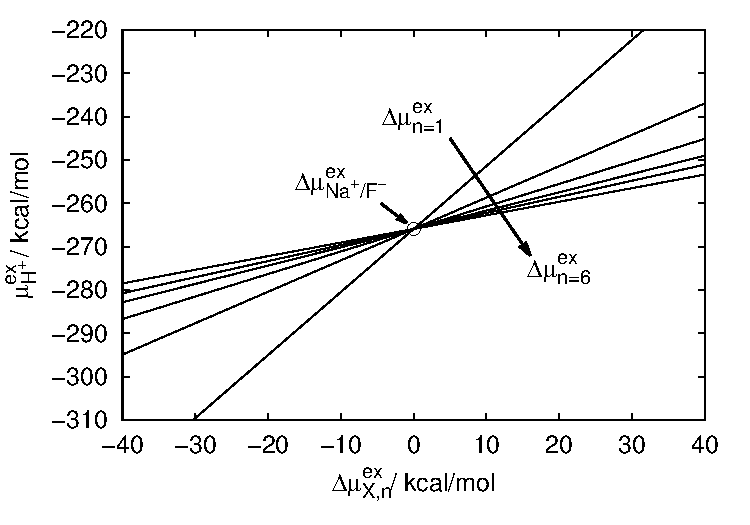
\includegraphics[width=0.98\linewidth]{images/cpa/cpa_example.pdf}
 \end{center}
\caption[Illustration of the cluster pair approximation for the proton solvation free energy]{Illustration of the cluster pair approximation for the
proton solvation free energy in the form described by Coe et al.\cite{coe1998cpa1}. Lines represent linear fits through all possible combinations of 
pairs and their differences (slopes taken directly from Ref. \cite{coe1998cpa1}). With increasing cluster size, the slope of the lines is reduced.
In the limit of \emph{n} $\rightarrow \infty$, the slope falls to zero defining $\mu\sursous{ex}{H\sur{+}}$. The lines also share an approximately 
common crossing point. This point sits very near the value of $\mu\sursous{ex}{H^{+}}$ even for \emph{n} = 1. Remarkable, really. The ion pair 
Na\sur{+} and F\sur{-} also sit very near the crossing point for \emph{n} = 1--6. By modeling the Na\sur{+} to F\sur{-} transition in 
$\mu\sursous{ex}{X,n}$ or other properties as a surrogate for the crossing point, I can test my prediction that the point will drift in response 
to the surface potential and other potential factors as \emph{n} becomes larger.}
\label{fig:coecpaexample}
\end{figure}

  This next point draws heavily from the discussion in the caption of \ref{fig:coecpaexample}. Two observations from the data presented in Refs. 
  \cite{coe1998cpa1} and \cite{kelly2006cpa} appear to support the CPA assumption. Figure 1 of Ref. \cite{coe1998cpa1} displays the cluster enthalpy 
  (obtained as in Figure \ref{fig:coecpaexample} for the free energy) vs \emph{n}$^{-1/3}$, showing an apparent convergence towards the bulk value with 
  increasing cluster size. Second, the slopes of the curves in Figure 1 of Ref. \cite{coe1998cpa1,kelly2006cpa,donald2010expand_cpa} are substantially 
  reduced by \emph{n} = 6. Ref. \cite{coe1998cpa1} suggests that, if there were to be any transition in the enthalpy or free energy values, it should occur 
  for intermediate cluster sizes. This is reasonable since $\Delta \mu^{ex}_{XW_n}$ approaches zero with increasing size, and thus from Eq. \ref{eq:cpa2}
  the proton enthalpy or free energy should approach an asymptotic (flat) form with increasing \emph{n}.

  Then for the large \emph{n} limit, 

  \begin{equation}
    \Delta \mu^{ex}_{X} = \lim_{n \rightarrow \infty} \Delta \mu^{ex}_{X,n}.
  \end{equation}

  Since I seek an estimate of $\Delta \mu^{ex}_{X}$ by calculating  $\Delta \mu^{ex}_{X,n}$, and the desired quantity refers to the change for an ion pair 
  in a large sample of water (with a distant liquid-vapor interface), for large clusters I constrain the ion location to the cluster center of mass in my 
  calculations. While this constraint leads to estimates of the thermodynamic quantities that do not accurately reflect the physical circumstance of ions 
  that are free to roam throughout the clusters, it serves to enhance the approach to large system behavior by ensuring that the ions are surrounded by 
  hydration shells that more closely mimic the bulk environment. I also compare this to calculations where the ion is free to roam the cluster as it will.

  To summarize, the discussion in this section located an extra-thermodynamic assumption in the original CPA approach\cite{coe1998cpa1} that allows for decoupling
  of salt hydration free energies, enthalpies, and entropies into single-ion contributions. The central assumption here is that the differences in these
  properties between microsolvated ions should rapidly converge for small \emph{n}, where the necessary input data is accessible to specialized mass spectrometric
  and theoretical analyses. Up to \emph{n} = 6, these differences appear to be converging towards the bulk limit and the \emph{real} proton solvation free energy, 
  etc. However, there is evidence to suggest that at some intermediate cluster size, the differences begin to drift in part due to solvation effects and in
  response to a more fully formed electrochemical surface potential. In Ref. \cite{pollard2014cpa1}, the shift is measured in each of $\Delta \mu^{ex}_{X,n}$,
  $\Delta h^{ex}_{X,n}$, and $\Delta s^{ex}_{X,n}$ by extending the cluster size out to \emph{n} = 105. In Ref. \cite{pollard2014cpa2}, the enthalpy expression
  is rewritten to solve for $\phi\sous{np}$ taking $\frac{1}{2}\Delta h^{ex}_{X,n}$ as input for the Na\sur{+} and F\sur{-} pair. This analysis reaches out to
  \emph{n} = 200 with direct comparison of the classical results to MP2-level quantum chemistry to \emph{n} = 35, and CCSD(T) to \emph{n} = 6 (triple-$\zeta$ basis)
  and 8 (double-$\zeta$ basis). The equation used to solve for the net potential is

  \begin{equation}
    \phi_{np}  = \frac{\Delta h_{X,b}^{ex}}{2}  + T\left(\frac{\partial \phi_{np}}{\partial T}\right)_P - \frac{\Delta h_{X,n}^{ex}}{2}.
    \label{eq:netpot2}
  \end{equation}
  
  \noindent $T\left(\frac{\partial \phi_{np}}{\partial T}\right)_P$ is taken as -9.9 cal/mol-K-\emph{e}\cite{randles1977structure} but I also use a value of
  0. cal/mol-K-\emph{e} based on the work outlined in Ref. \cite{pollard2014cpa1}. An expression starting from the free energy exists as well
  
  \begin{equation}
    \phi_{np} = \frac{(\Delta \mu_{X,b}^{ex} - \Delta \mu_X^{ex})}{2}.
    \label{eq:netpot1}
  \end{equation}

  \noindent The surface potential itself is not present in the entropy, only its temperature derivative is present, refer to Eq. \ref{eq:echems}.
  
  Computationally the differences can be evaluated as in Eqns. \ref{eq:dechemmu}--\ref{eq:dechems}
  
  \begin{equation}
    \Delta \mu_X^{ex} = \Delta \mu_{X,b}^{ex} - 2\phi_{np}
    \label{eq:dechemmu}
  \end{equation}

  \begin{equation}
    \Delta h_X^{ex} = \Delta h_{X,b}^{ex} - 2\phi_{np} + 2T\left(\frac{\partial \phi_{np}}{\partial T}\right)_P
    \label{eq:dechemh}
  \end{equation}

  \begin{equation}
    \Delta s_X^{ex} = \Delta s_{X,b}^{ex} + 2\left(\frac{\partial \phi_{np}}{\partial T}\right)_P
    \label{eq:dechems}
  \end{equation}
  
  \noindent The bulk differences in these equations come from Marcus\cite{marcus1985book} and some relevant pairs are given in Table \ref{tab:marcus}.

  \begin{table}
   \begin{center}
    \begin{tabular}{lrrrrr}
     \hline
     \hline
      & Li$^+$ & Na$^+$ & K$^+$ & Rb$^+$ & Cs$^+$ \\
     \hline
     \\
     \multicolumn{6}{c}{$\Delta\mu^{ex}_{X,b}$  (kcal/mol)} \\
     \\
      F$^-$ & 2.2 & -23.2 & -40.2 & -45.7 & -51.1 \\
      Cl$^-$ & 32.0 & 6.7 & -10.3 & -15.8 & -21.3 \\
      Br$^-$ & 38.2 & 12.9 & -4.1 & -9.6 & -15.1 \\
      I$^-$ & 47.3 & 22.0 & 5.0 & -0.5 & -6.0 \\
     \\
     \multicolumn{6}{c}{$\Delta h^{ex}_{X,b}$  (kcal/mol)} \\
     \\
      F$^-$ & 0.7 & -26.8 & -46.6 & -52.6 & -58.6 \\
      Cl$^-$ & 34.9 & 7.4 & -12.4 & -18.4 & -24.4 \\
      Br$^-$ & 42.3 & 14.8 & -5.0 & -11.0 & -17.0 \\
      I$^-$ & 53.1 & 25.6 & 5.7 & -0.2 & -6.2 \\
     \\
     \multicolumn{6}{c}{$\Delta s^{ex}_{X,b}$ (cal/mol-K)} \\
     \\
      F$^-$ & -5.0 & -12.0 & -21.3 & -23.0 & -25.0 \\
      Cl$^-$ & 9.7 & 2.3 & -7.0 & -8.7 & -10.3 \\
      Br$^-$ & 13.7 & 6.3 & -3.0 & -4.7 & -6.3 \\
      I$^-$ & 19.3 & 12.0 & 2.3 & 1.0 & -0.7 \\
     \hline
     \hline
    \end{tabular}
   \end{center}
   \caption[Ion pair differences in the bulk thermodynamic quantities]{Marcus bulk free energy, enthalpy, and entropy difference data.\cite{marcus1985book}}
   \label{tab:marcus}
  \end{table}

  \section{\label{ch5:sec2:level1}Computational methods}
  The work in Ref. \cite{pollard2014cpa2} builds on that done in Ref. \cite{pollard2014cpa1}, so I'll focus principally on this second study.
  
  The molecular dynamics package Tinker\cite{ponder2004tinker} was used to perform simulations of ion-water clusters with the polarizable AMOEBA force field\cite{amoeba};
  the sodium and fluoride ions were studied. Cluster sizes were estimated assuming a density of 0.997 g cm$^{-3}$ for a cluster of \emph{n} waters. A half-harmonic 
  bounding potential was applied a further 2.0 \AA~beyond the computed size to reflect any evaporating waters back into the cluster. The default AMOEBA bonded and 
  nonbonded parameters were assigned to sodium and all waters. In the case of fluoride, the Thole damping parameter was reduced from 0.39 to 0.2, having the effect 
  of bringing the ion induced dipole distribution into better agreement with quantum mechanical calculations performed 
  previously\cite{masia2009polarize,rogers2010ctpolar,baer2011toward}. Simulations were also performed with the default values for comparison. 
  
  The simulations were carried out at a temperature of 300 K for 6 ns with all nonbonded cutoffs removed. In one set of calculations each ion was free to explore the
  extent of the droplet. A second set of calculations freezes the ion at the droplet center of mass with the aim of accelerating convergence of the solvation behavior
  to the bulk limit. For subsequent quantum chemical analysis, 500 configurations from each case were extracted from the trajectory.
  
  Dynamics using the B3LYP-D3/6-31++G(d,p)\cite{grimme2010d2} potential energy surface as implemented in the QChem 4.0.1 package\cite{shao2006qchem,krylov2013qchem} was
  performed for clusters of \emph{n}=1--6 waters about a sodium or fluoride ion. Four simulations were performed for 36 ps under constant energy conditions for each
  cluster/ion pair. The initial velocities were randomly generated from a Boltzmann kinetic energy distribution; the same initial configuration was employed for each
  run and 12 ps of the dynamics was discarded to allow for deviation of the cluster state due to the differing initial velocities. No external potential was used for
  these simulations. From each of these trajectories, 250 configurations were extracted and energies were computed at the B3LYP-D3/6-31++G(d,p) and
  RI-MP2/aug-cc-pVDZ/aug-cc-pVDZ-RI levels of theory.
  
  Extending the analysis of Ref. \cite{pollard2014cpa1} to the quantum chemical level requires extensive computational resources. Determination of $\phi_{np}$ through 
  enthalpy differences as in Equation \ref{eq:netpot2} is particularly direct, however, requiring only calculation of cluster energies and the energy of the ion with
  the dimer-centered basis set to account for basis set superposition errors. For larger clusters, these calculations become more difficult as the differences being
  sought become very small compared to the magnitude of the energies involved. For the current study, all energies were computed using the Psi4 quantum chemistry 
  software (beta version 5)\cite{sherrill2012psi4}. These were done at the RI-MP2/aug-cc-pVDZ/aug-cc-pVDZ-RI level of theory considering nearest noble gas frozen core
  approximation and neglecting zero point contributions.
  
  As mentioned in the previous section, the MP2-level calculations came under fire because MP2 is known to overestimate dispersion interactions\cite{tkatchenko2009dispersion}.
  This is the reason I used spin-component scaled MP2\cite{grimme2003scsmp2} in Chapter \ref{ch3:sec1:level1}. By rescaling the same-spin and opposite-spin components
  of the MP2 energy, I can more accurately dial in the dispersion energy compared to higher levels of theory. However, for the purposes of addressing these concerns,
  I have chosen to use the `gold standard' quantum chemistry method of CCSD(T). To that end, I also include unpublished calculations performed on a subset of the initial 
  500 configurations for each Na/water and F/water cluster size. Some 30 configurations were chosen so as to reproduce the mean and standard deviation of the larger population
  to within 0.05 kcal/mol for a particular cluster size using the existing RI-MP2/aug-cc-pVDZ data. I use Cholesky decomposition instead of the conventional resolution-of-the-identity
  approximation to speed up the calculation of the repulsion integrals. The Cholesky decomposition tolerance was set to 5e-6 for CCSD(T)/aug-cc-pVDZ and CCSD(T)/jun-cc-pVTZ calculations. 
  This however is quite prohibitive in probing CCSD(T) energies for larger clusters, so I was only able to perform the calculations on clusters with up to \emph{n} = 6 waters 
  (jun-cc-pVTZ basis) and \emph{n} = 8 waters (aug-cc-pVDZ basis).
  
  \section{\label{ch5:sec3:level1}Results}

  \subsection{\label{ch5:sec3:level2}Drift in $\mu\sursous{ex}{X,n}$, $h\sursous{ex}{X,n}$, and $s\sursous{ex}{X,n}$ as \emph{n} $\rightarrow \infty$}

  Refer to Table \ref{tab:clusterdata} for a discussion of the results from Ref. \cite{pollard2014cpa1} beginning with the Na$^+$/F$^-$ pair in the \emph{n} = 5 water cluster. 
  The results for the cation to anion free energy and enthalpy changes agree with experiment within a range that is of the same magnitude as the difference between the listed 
  experimental values. Throughout the calculations, the expected errors in the calculated free energy differences are estimated to be in the range 0.5 to 1.0 kcal/mol, while 
  the enthalpy difference errors are small for the \emph{n} = 5 cluster (0.1 kcal/mol) and larger for the \emph{n} = 25 and \emph{n} = 105 cases (1 to 1.5 kcal/mol). The 
  small-cluster results suggest that the AMOEBA model (with the reduced polarization parameter) represents the local ion-water interactions with decent accuracy for the 
  Na$^+$/F$^-$ pair.

  \begin{table}
   \begin{center}
    \begin{tabular}{lrrrrrr}
     \hline
     \hline
      Ion Pair & Size & $\Delta\mu^{ex}_{X,n}$ & $\Delta h^{ex}_{X,n}$ & $\Delta s^{ex}_{X,n}$ 
      & $\phi_{np}$  & $\partial \phi_{np} / \partial T$ \\
     \hline
      NaF(expt\cite{donald2010expand_cpa}) & 5 & -1.5 & -0.5 & 3.3   & & \\
      NaF(expt\cite{coe1998cpa1}) & 5 & -0.1 & 2.7 & 9.3   &  & \\
      RbI(expt\cite{coe1998cpa1,donald2010expand_cpa}) & 5 & 12.1 & 15.7 & 12.0   &  & \\
      NaF & 5 & 0.8 & 0.1 & -2.3 & &  \\
      RbI & 5 & 9.8 & 9.6 & -0.7 & &  \\
      NaF & 25 & -2.6 & -8.0 & -18.0 & -10.3 & -3.0 \\
      RbI & 25 & & 25.4 & &   -13.6 & \\
      RbI & 45 & & 21.6 & &  -11.7  & \\
      NaF & 105 & -3.1 & -8.2 & -17.0 & -10.1  & -2.5 \\
      RbI & 105 & 15.1 & 15.5 & 1.3 &  -7.8 & 0.2 \\
      RbI & 242 & 14.2 &     & &  -7.4      & \\
     \hline
     \hline
    \end{tabular}
   \end{center}
   \caption[Cluster data for NaF and RbI pairs]{Cluster data from AMOEBA simulations and experiment\cite{coe1998cpa1,donald2010expand_cpa} All values are in kcal/mol except 
   for the $\Delta s^{ex}_{X,n}$ and $\partial \phi_{np} / \partial T$ results, which are in cal/mol-K. The net potential values are computed using Eq. \ref{eq:netpot1}. 
   The proton hydration free energy, enthalpy, and entropy derived using the above data are -264.7 kcal/mol, -271.9 kcal/mol, and -24.0 cal/mol-K, respectively. The 
   corresponding values from Ref. \cite{coe1998cpa1} are -265.9 kcal/mol, -274.9 kcal/mol, and -30.0 cal/mol-K.}
   \label{tab:clusterdata}
  \end{table}

  For the Na$^+$/F$^-$ pair in the \emph{n} = 25 water cluster, there is a shift in the free energy difference (-2.6 kcal/mol) and a larger shift in the enthalpy difference 
  (-8.0 kcal/mol). The computed entropy difference is seen to be large and negative, exhibiting a compensating effect between enthalpy and entropy.  The entropy change implies 
  that, for the F$^-$ ion, the second hydration shell has more induced order due to interactions with the ion and first shell waters relative to the Na$^+$ ion.

  Approaching the bulk limit with a cluster size of \emph{n} = 105, free energy and enthalpy differences do not change significantly from the \emph{n} = 25 results. This 
  suggests that, already with a second hydration shell, bulk-like behavior is emerging for the cation/anion difference (for this kosmotropic pair). The agreement of the 
  \emph{n} = 25 cluster results with the larger-cluster limit will be exploited in quantum mechanical calculations of the same quantities in the next section.

  The computed temperature derivative of the net potential (from Eq. \ref{eq:dechems}), is -2.5 cal/mol-K-\emph{e} for the \emph{n} = 105 cluster. This value has the same sign
  but is reduced in magnitude by roughly a factor of 4 from the value reported by Randles\cite{randles1977structure} and \cite{hunenberger2011sp} based on a range of experiments.  
  It's unknown whether this discrepancy is due to the experimental values being inaccurate (discussion on this possibility in Ref. \cite{hunenberger2011sp}), the curvature of
  the small clusters used here changing the derivative, or the AMOEBA model simply not doing a good job reproducing this property. Fair to say, it might be all of the above, but
  it is suspected that the experimentally derived derivative is too negative\cite{donald2010expand_cpa}. I elaborate on this a bit more in the next section as well.

  The derived net potential (at 300 K) from this data is -10.1 kcal/mol-\emph{e} or -0.44 V. It is interesting that I observe a negative net potential along with the negative 
  temperature derivative. If anything, at higher temperatures the derivative should become more positive because the cavity/water boundary behaves much like a hydrophobic 
  particle which has a positive hydration entropy.

  While examining the Marcus bulk values\cite{marcus1985book} for alkali halide ion pairs (Table \ref{tab:marcus}), it was observed that the chaotropic Rb$^+$/I$^-$ ion pair 
  displays near-zero values for the differences of the bulk (Marcus) free energies and enthalpies; this contrasts with the Na$^+$/F$^-$ case that exhibits a near-zero value for 
  the small cluster free energy difference in the CPA\cite{coe1998cpa1}. In Eqns. \ref{eq:netpot2} and \ref{eq:dechemh}, this suggests that the enthalpy change is nearly entirely 
  a net potential effect, or conversely, the net potential comes primarily from the large-cluster enthalpy change (since the term involving the temperature derivative of the net 
  potential is only of magnitude in the range $\sim$0 to -3 cal/mol, based on the results reported here and experimental estimates\cite{randles1977structure}). Simulations were 
  also performed of the Rb$^+$/I$^-$ pair. Clusters of sizes \emph{n} = 5, 25, 45, 105, and 242, since this ion pair displays slower convergence with increasing cluster size. 

  The Rb$^+$/I$^-$ pair yields several interesting results. First, the computed free energy difference for the \emph{n} = 5 cluster is 2.3 kcal/mol smaller than the experimental 
  value, while the computed enthalpy difference is 6.1 kcal/mol smaller than the experimental value (suggesting deficiency in the AMOEBA ion-water interactions for this ion pair). 
  Second, the enthalpy differences for the \emph{n} = 25 and \emph{n} = 45 clusters and the \emph{n} = 105 cluster differ substantially, suggesting convergence is not reached until
  larger cluster sizes for the chaotropic pair. Third, the free energy difference for the \emph{n} = 105 cluster is quite close to the enthalpy difference, indicating a small entropy
  difference. The net potential obtained for this very different ion pair is consistent with that for the Na$^+$/F$^-$ pair (negative and of substantial magnitude), but differing 
  by 2.3 kcal/mol-\emph{e}. Applying an \emph{ad hoc} correction of 2.3 kcal/mol due to the deviation from experiment for the \emph{n} = 5 cluster, the net potential becomes -9.0
  kcal/mol-\emph{e}, in agreement with the result using the NaF pair. Fourth, the \emph{n} = 242 free energy difference and the resulting net potential confirm that the results 
  are relatively well converged by \emph{n} = 105. Compare this with the kosmotropic pair where these properties were seemingly converged by \emph{n} = 25.

  Using Eq. \ref{eq:cpa1} (and the corresponding enthalpy equation), the predicted values for the proton hydration quantities taken as averages between the kosmotropic and corrected
  chaotropic pairs are: $\mu\sursous{ex}{H\sur{+}}$ -264.7 kcal/mol, $h\sursous{ex}{H\sur{+}}$ -271.9 kcal/mol, and $s\sursous{ex}{H\sur{+}}$ -24.0 cal/mol-K. The net potential is
  estimated (also as an average of the two measurements) as -10.4 kcal/mol-\emph{e} or -0.45 V. The 6.1 kcal/mol correction to the enthalpy for the RbI pair is probably too large
  as the resulting entropy prediction is -28.3 cal/mol-K. It is expected that with the small but still negative prediction of the temperature derivative discussed above, the average
  would be more positive than the Marcus value of -24 cal/mol-K\cite{marcus1985book}.

  The shifts in the free energy and enthalpy are due to 1) sequential hydration effects and 2) the net potential effect. These effects work in opposite directions, so if the shifts 
  were due entirely to a net potential effect, free energy and enthalpy shifts in the opposite direction would be observed for the Na$^+$F/$^-$ pair. This suggests a significant 
  contribution from sequential hydration effects in which the first shell strongly interacts with the second shell (with a corresponding large negative value for the entropy for the
  F$^-$ ion). This effect is apparently large enough to overcome the shift in the opposite direction due to the net potential. For the Rb$^+$/I$^-$ pair, on the other hand, the net 
  potential effect on the enthalpy difference is largely isolated due to the small value of the bulk enthalpy difference in Eq. \ref{eq:dechemh}. The net potential is very small for
  clusters of \emph{n} = 5 (on the order of about 10\% as large). For RbI, the shift is due to the emergence of the remaining 90\% of the potential as the free energy differences 
  due to the ion specific hydration effects cancel. The Rb$^+$/I$^-$ results provide a further indication of the stronger hydration of anions relative to cations (for a given ion 
  size), reflected in the nearly equal bulk hydration free energies but smaller radius of the Rb$^+$ ion compared with the I$^-$ ion. 
  
  Given the issues with the RbI pair, the value of $\Delta h^{ex}_{X,n}$ is adapted from Ref. \cite{coe1998cpa1} which is 15.7 kcal/mol for \emph{n} = 5. The slope of this line is
  $\Delta h^{ex}_{X}/2\Delta h^{ex}_{X,n}$ and is equal to 0.64. Rearranging to solve for $\Delta h^{ex}_{X}$, the CPA estimate is 20.1 kcal/mol (which is reduced from the 21.6 
  kcal/mol from the simulation results). This difference gives a new net potential of -10.1 kcal/mol-\emph{e} with the temperature derivative set to zero and -13 kcal/mol-\emph{e}
  when set to -9.9 cal/mol-K-\emph{e}. Either way, it is clear that the net potential is negative and is of large magnitude. The -13 kcal/mol-\emph{e} potential with a -9.9 cal/mol-K-\emph{e}
  temperature derivative being larger than that predicted by Ashbaugh et al.\cite{ashbaugh2008lps} also suggests that the temperature dependence of the net potential may be smaller 
  than is currently accepted\cite{randles1977structure,hunenberger2011sp}.

  \subsection{\label{ch5:sec3:level3}Size dependence of ion-pair enthalpy differences}
  For my analysis of the size dependence of ion-pair enthalpy differences, I start by examining the small-cluster size range (\emph{n} = 1--6 water molecules) for the NaF 
  ion pair. With the modified Thole parameter, Figure \ref{fig:dHexptsmall} shows excellent agreement of the computed enthalpy difference with the experimental values
  listed in Ref. \cite{donald2010expand_cpa} (except for a deviation for the \emph{n} = 1 case). Using the default Thole parameter results in significant deviation 
  from experiment for the \emph{n} = 2--6 clusters. The small cluster data tabulated in Ref. \cite{donald2010expand_cpa} includes a wider range of experimental studies
  than in the original CPA paper\cite{coe1998cpa1}.

  Examination of radial distribution functions (RDFs, not shown) for the F$^-$ ion/water(oxygen) pair shows that reduction of the Thole parameter leads to an increase in the 
  average ion-water oxygen distance of 0.25 {\AA}. Related to this structural observation, Ref. \cite{kawashima2013ab} presents fundamental simulations of \emph{n} = 1--3 F$^-$/water
  clusters. The electrons are treated at the MP2 level, while the nuclear motions include quantum effects through path integral simulations. The results show a 
  significant broadening of the RDFs for the \emph{n} = 3 cluster with a substantial tail developing at large distances (and some increased density at small distances) due to
  nuclear quantum effects. (Note that the ion/hydrogen and ion/oxygen RDFs are mislabeled in Ref. \cite{kawashima2013ab}.)

  This suggests that the reduced Thole parameter has two effects: 1) production of a more realistic polarization state of the F$^-$ ion and 2) a larger bond length that 
  fortuitously mimics the inclusion of nuclear quantum effects; both then lead to better agreement with experiment for the enthalpy differences.  It is interesting
  that, in the results of Ref. \cite{kawashima2013ab}, a large distance tail is not observed for the \emph{n} = 1 case; in fact, when nuclear quantum effects are included, 
  the distributions display some contraction to smaller ion-water distances. This may explain the deviation of the \emph{n} = 1 modified AMOEBA results in Figure 
  \ref{fig:dHexptsmall} from experiment, and the better agreement of the default AMOEBA model. The results in Ref. \cite{kawashima2013ab} also suggest that water-water
  interactions are important, even for the small \emph{n} = 2--6 clusters. 
  
\begin{figure}
 \begin{center}
  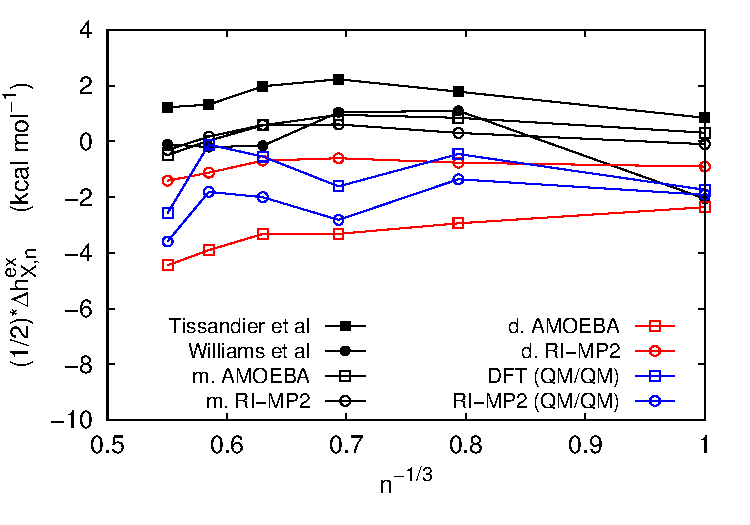
\includegraphics[width=0.98\linewidth]{images/cpa/deltaH_exptl_range-eps-converted-to.pdf}
 \end{center}
\caption[Half the enthalpy differences in the Na\sur{+}$\rightarrow$F\sur{-} transition for small clusters]{Half the difference in the enthalpy for the Na$^+$ to 
F$^-$ transition in the \emph{n} = 1--6 clusters. All simulations allowed free motion of the ions in the clusters. The plot labeled ``Tissandier'' (black solid squares) is 
for experimental data from Ref. \cite{coe1998cpa1}, and the plot labeled ``Williams'' (black solid circles ) is for experimental data from Ref.
\cite{donald2010expand_cpa} obtained from a larger range of experiments. ``m. AMOEBA'' (black open squares) refers to results from the modified AMOEBA model, while 
for ``m. RI-MP2'' the energies were computed at the MP2 level (with modified AMOEBA sampling). ``d. AMOEBA'' (red open squares) indicates the default AMOEBA model, 
and ``d. RI-MP2'' (red open circles) is for energies computed at the MP2 level (with default AMOEBA sampling). ``DFT(QM/QM)'' (blue open squares) labels the DFT
simulation results, and ``RI-MP2(QM/QM)'' (blue open circles) indicates DFT sampling with energy calculations at the MP2 level. The cluster size is displayed as 
n$^{-1/3}$.}
\label{fig:dHexptsmall}
\end{figure}

  To further explore the role of electronic quantum effects in the small clusters, I computed enthalpy differences for several other cases. First, I generated
  configurations with both the modified and default Thole parameter simulations, and computed the energies at the MP2 level. The MP2-computed enthalpy differences
  (using the modified Thole parameter for the sampling) accurately match the modified AMOEBA results. When the default Thole parameter is used to generate the
  configurations, the MP2 results lie between the default AMOEBA results and experiment. 
  
  Finally, configurations were also generated with B3LYP-D3/DFT simulations. When the energies are computed at the same level of theory, it is apparent the quantum
  model yields results more negative than experiment (except for the \emph{n} = 5 case). It is interesting that, when energies are computed at the MP2 level (with DFT
  configurations), larger deviations from experiment are observed. Nuclear quantum effects were not included in the DFT simulations, and based on the discussion 
  above these would likely move the computed values upward toward the experimental results. It is important to note the AMOEBA model was parametrized based on MP2 
  level calculations (with no inclusion of nuclear quantum effects)\cite{amoeba}. From the above results, I can conclude that the modified AMOEBA model
  for the F$^-$ ion yields quite accurate results for the energetics of the cation to anion transition in the small clusters. 

  Next I'll explore the size dependence of the cation-anion enthalpy difference over a large range of cluster sizes (up to \emph{n} = 200). As in Ref. \cite{pollard2014cpa1}, 
  I first constrain each ion to the cluster center of mass for clusters of \emph{n} $\geq$ 5. Figure \ref{fig:dHcom} displays the enthalpy difference as a function 
  of cluster size using the modified AMOEBA model and MP2 calculations. First, it is clear that a shift to more negative values develops as the cluster size is 
  increased beyond \emph{n} = 6. The shift appears to stabilize (with some oscillation) at a value of roughly $-4$ kcal/mol; already by the \emph{n} = 10 cluster size, 
  the majority of the shift has occurred. This is just beyond the scope of the myriad CPA studies\cite{coe1998cpa1,coe2001cpa2,coe2002cpa3,donald2010expand_cpa,kelly2006cpa}
  but still within the range of both experimental and theoretical used to generate the smaller cluster data\cite{wheeler2015hydration}.
  
\begin{figure}
 \begin{center}
  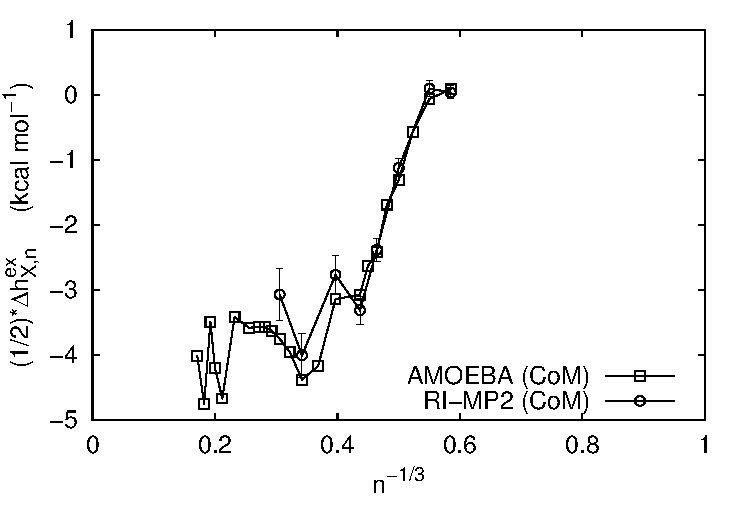
\includegraphics[width=0.98\linewidth]{images/cpa/deltaH_com-eps-converted-to.pdf}
 \end{center}
\caption[Half the enthalpy differences in the Na\sur{+}$\rightarrow$F\sur{-} transition for clusters with the ion fixed at the center of mass]{Half the difference 
in the enthalpy for the the Na$^+$ to F$^-$ transition in larger clusters (up to \emph{n} = 200). The energies were computed from modified (reduced Thole factor) AMOEBA
trajectories block-averaging every 100 steps for the case of the ion bound to the cluster center of mass (CoM). The results are compared out to \emph{n} = 35 with a sample 
of configurations modeled at the RI-MP2/aug-cc-pVDZ/aug-cc-pVDZ-RI level of theory. The cluster size is given as \emph{n}$^{-1/3}$. Error bars for AMOEBA averages are smaller
than the size of the symbols.}
\label{fig:dHcom}
\end{figure}

  In Ref. \cite{pollard2014cpa1} there was some discussion of the difficulties in obtaining converged enthalpy differences for the larger cluster sizes (involving the 
  difference of two large numbers and possible partial evaporation events). However, the previous free energy results (which are less affected by the difficulties in 
  the enthalpy calculations) fully support the notion that the net potential stabilizes for clusters in the size range considered here.  

  There is remarkable agreement of the MP2 results out to \emph{n} = 35 with the classical results. Since the configurations were generated with the modified AMOEBA model, 
  perhaps this is not so surprising; it does show that, for a given set of configurations, the model accurately mimics the energetics obtained from the realistic
  quantum electron distribution. The configurations are for the ions fully coupled to the nearby waters, and do not rely on a particular cavity definition.  

  The agreement of the modified AMOEBA results with experiments on small clusters discussed above then suggests this model is accurately representing the energetics
  over the full size range. It seems highly unlikely that errors in half the enthalpy difference of magnitude 10 kcal/mol occur (pushing the asymptotic values of the
  curves in Figures \ref{fig:dHcom} and \ref{fig:dHfree} downward by $\approx 10$ kcal/mol); such a shift magnitude would be necessary to produce a net potential 
  close to zero. 

  For the case in which the ions are free to move about the entire cluster, similar results are obtained (Figure \ref{fig:dHfree}). The enthalpy differences first
  stabilize at a slightly higher energy relative to Figure \ref{fig:dHcom}, but then relax to the asymptotic value of $-4$ kcal/mol. Again, the quantum results are 
  very close to the AMOEBA results.  The results show that locating the ion at the cluster center (aimed at more rapid convergence to the bulk limit) has only a 
  small effect on the computed results for this kosmotropic ion pair.  

\begin{figure}
 \begin{center}
  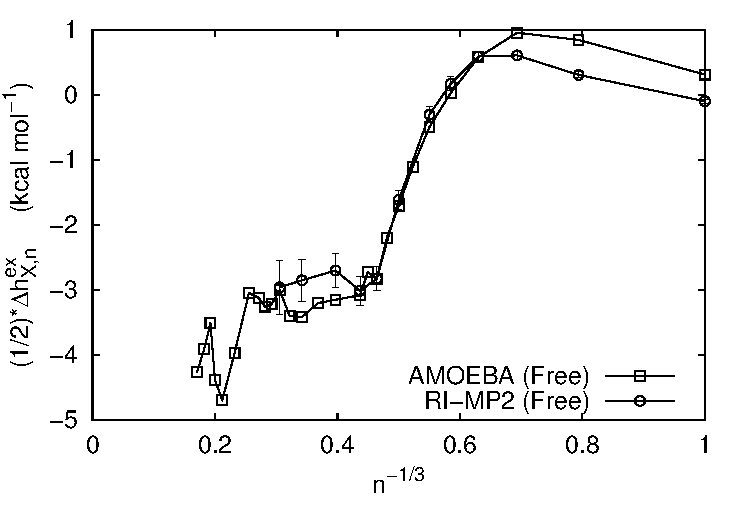
\includegraphics[width=0.98\linewidth]{images/cpa/deltaH_free-eps-converted-to.pdf}
 \end{center}
\caption[Half the enthalpy differences in the Na\sur{+}$\rightarrow$F\sur{-} transition for clusters with the ion unconstrained]{Half the difference in the enthalpy 
for the the Na$^+$ to F$^-$ transition in larger clusters (up to \emph{n} = 200). The energies were computed from modified (reduced Thole factor) AMOEBA trajectories
block-averaging every 100 steps for the case of the ion free to move throughout the cluster. The results are compared out to \emph{n} = 35 with a sample of configurations
modeled at the RI-MP2/aug-cc-pVDZ/aug-cc-pVDZ-RI level of theory. The cluster size is given as n$^{-1/3}$. Error bars for AMOEBA averages are smaller than the size of
the symbols.}
\label{fig:dHfree}
\end{figure}

  Considering the extension of these differences to the `gold standard' CCSD(T) method, I found similar agreement to that which I established earlier between AMOEBA
  and the MP2 method, see Figure \ref{fig:dHfreeall}. Out to a size of \emph{n} = 3, the quantum results fall more negative than the AMOEBA result at an intermediate
  energy to that predicted by Tissandier et al. and Williams et al. in Refs. \cite{coe1998cpa1} and \cite{donald2010expand_cpa}, respectively. Interestingly, there
  seems to be better overlap between the CCSD(T)/jun-cc-pVTZ and MP2 trends than when using CCSD(T)/aug-cc-pVDZ implying a fortuitous result at the lower level of 
  theory which is of similar quality to the much more prohibitive triple-$\zeta$ coupled-cluster method. Most importantly however, each of the trends tracks the drift
  in the Na\sur{+}/F\sur{-} pair enthalpy differences from near zero.

\begin{figure}
 \begin{center}
  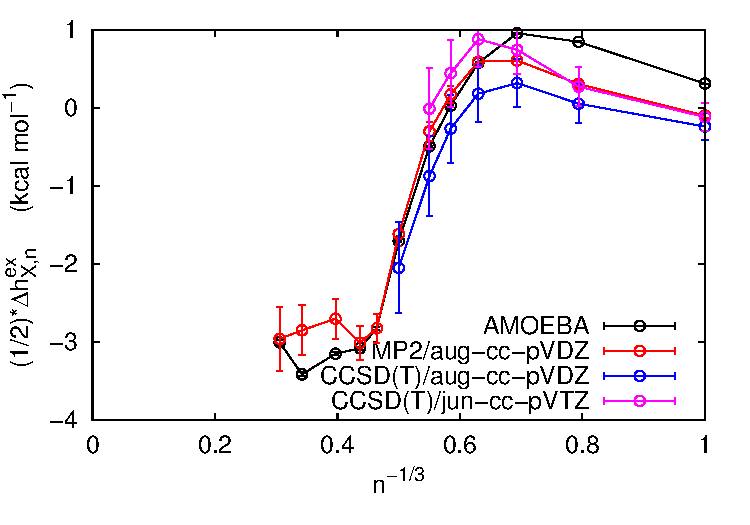
\includegraphics[width=0.98\linewidth]{images/cpa/deltaH_all-eps-converted-to.pdf}
 \end{center}
\caption[Half the enthalpy differences in the Na\sur{+}$\rightarrow$F\sur{-} transition at several levels of theory]{Half the enthalpy differences in the transition of 
Na $\rightarrow$ F, expressed in kcal/mol across varying theoretical treatments for clusters with up to \emph{n} = 35.}
\label{fig:dHfreeall}
\end{figure}

  A comparison between the AMOEBA and MP2 energies to the higher levels of theory revealed that the bulk of the figures fall within $\pm$ 0.5 kcal/mol of the higher 
  level estimate, see Figure \ref{fig:dHfreediffs}. The AMOEBA model tended to produce more positive energies than CCSD(T) except beyond \emph{n} = 3 for CCSD(T)/jun-cc-pVTZ, 
  while MP2 was slightly more negative than CCSD(T)/jun-cc-pVTZ and more positive than CCSD(T)/aug-cc-pVDZ. Differences between the AMOEBA and quantum methods tended to
  exhibit non-linear fluctuations while those between MP2 and CCSD(T) were approximately linear over the range considered. Overall, however, I find remarkable agreement
  between the methods.

\begin{figure}
 \begin{center}
  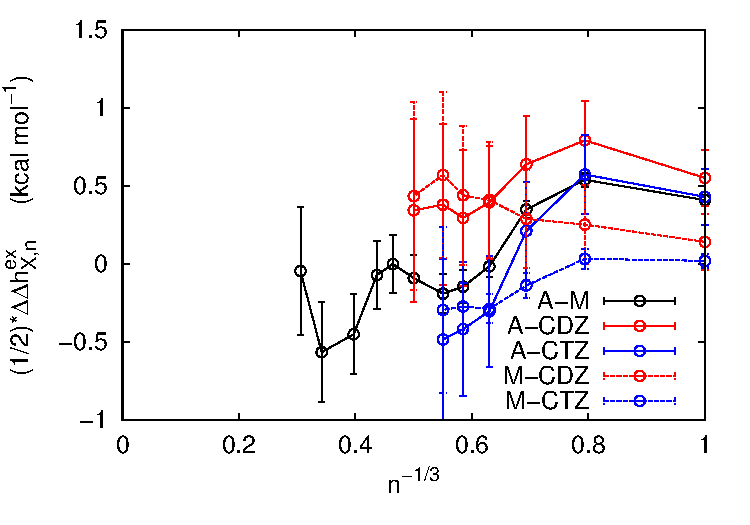
\includegraphics[width=0.98\linewidth]{images/cpa/deltaH_diffs_all-eps-converted-to.pdf}
 \end{center}
\caption[Differences in $\frac{1}{2}h\sursous{ex}{X,n}$ between methods]{Comparison of $\frac{1}{2}\Delta h\sursous{ex}{X,n}$ for the the Na$^+$ to F$^-$ transition, expressed
in kcal/mol between the various methods, 1) AMOEBA minus MP2/DZ, 2) AMOEBA minus CCSD(T)/DZ, 3) AMOEBA minus CCSD(T)/TZ, 4) MP2/DZ minus CCSD(T)/DZ, and 5) MP2/DZ minus
CCSD(T)/TZ. A is shorthand for AMOEBA, M for MP2, CDZ for CCSD(T)/DZ, and CTZ for CCSD(T)/TZ. DZ and TZ refer to aug-cc-pVDZ and jun-cc-pVTZ basis sets, respectively.}
\label{fig:dHfreediffs}
\end{figure}

  Projecting the MP2 to CCSD(T) errors to the bulk limit, assuming the \emph{n}$\sur{-\frac{1}{3}}$ dependence remains linear, it is clear that the errors in the reported
  enthalpy differences aren't likely to exceed 1 kcal/mol, see Figure \ref{fig:ccsdterror}. Granted, the trend approaches an asymptotic limit of about -4 kcal/mol at large 
  \emph{n}. However, even the AMOEBA to MP2 differences start off relatively linearly before oscillating in the range of $\pm$0.5 kcal/mol from zero. It's likely given that
  AMOEBA was parameterized against MP2 that the MP2 to CCSD(T) errors will also start to oscillate, making the linear projection a sort of \emph{worst case scenario}. Errors
  assuming the linear and oscillatory trends are discussed below.

\begin{figure}
 \begin{center}
  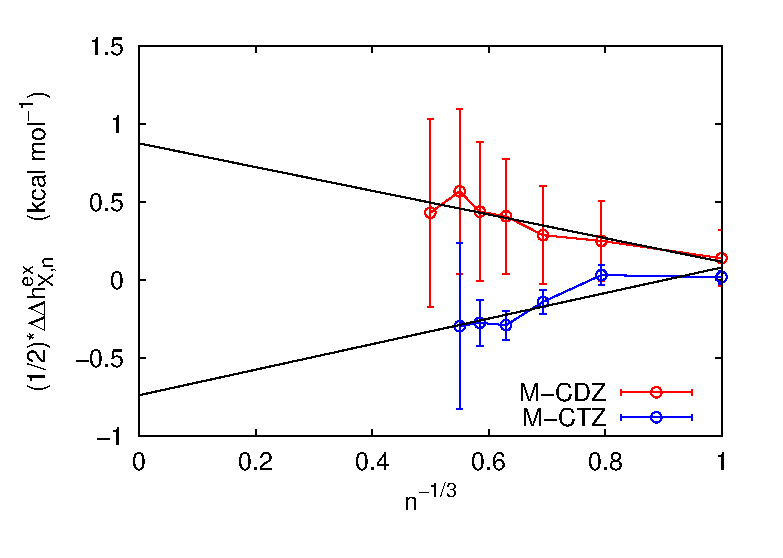
\includegraphics[width=0.98\linewidth]{images/cpa/deltaH_ccsdt_fit.eps}
 \end{center}
\caption[Estimated error in the MP2-level enthalpy relative to CCSD(T)]{Differences in $\frac{1}{2}\Delta h\sursous{ex}{X,n}$ (MP2 minus CCSD(T)) in the transition of Na 
$\rightarrow$ F, expressed in kcal/mol. Here M is shorthand for MP2, CDZ for CCSD(T)/aug-cc-pVDZ, and CTZ for CCSD(T)/jun-cc-pVTZ. The solid black lines are linear fits 
through the data and provide an estimate of the error in the enthalpy shift to large cluster size.}
\label{fig:ccsdterror}
\end{figure}

  Using Equation \ref{eq:netpot2}, I display in Figure \ref{fig:netpotsim} the size dependence of the derived net potential. As discussed above, I assume a
  temperature derivative of the net potential of zero. It is clear from the plot that the net potential approaches an asymptotic value of close to $-9.4$ kcal/mol-$e$
  discussed in Refs. \cite{beck2013sp} and \cite{pollard2014cpa1}. Compare this with the result assuming the -9.9 cal/mol-K-\emph{e} temperature derivative in Figure
  \ref{fig:netpotlps}. Given my discussion of the errors previously, it is instructive to note that the nearest alternative estimate of the electrochemical surface 
  potential is +3 kcal/mol-\emph{e} (+0.13 V). The linear estimate produces a 25\% error in my estimate of $\phi\sous{np}$ with a lower limit of $\approx~$-6.8 kcal/mol-\emph{e}. 
  Taking the oscillations of the AMOEBA to MP2 trend as an estimate of the error instead, I expect a more realistic uncertainty of -9.4 $\pm$ 1.1(25) kcal/mol-\emph{e} which
  is half the estimate of the \emph{worst case scenario} spelled out above. In volts that's -0.41 $\pm$ 0.05 V, though I always round down to -0.4 V.
  
\begin{figure}
 \begin{center}
  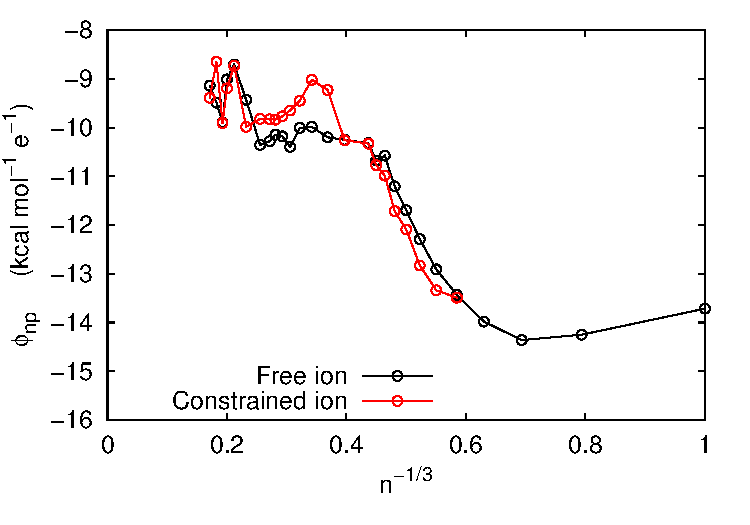
\includegraphics[width=0.98\linewidth]{images/cpa/net_pot_no_temp_deriv-eps-converted-to.pdf}
 \end{center}
\caption[Net potential with no temperature derivative]{The electrochemical surface potential as a function of cluster size up to \emph{n} = 200 (using Equation \ref{eq:netpot2}).
The temperature derivative ofthe net potential was assumed to be zero, as discussed in the text. The plots are for the cases in which the ions was either restricted to the
cluster center of mass or free to move throughout the cluster. The F$^{-}$ Thole damping parameter has been reduced from the default 0.39 value to 0.2 in generating the trajectories. 
The cluster size is given as n$^{-1/3}$. Error bars are comparable to or smaller than the size of the points (approximately $\pm$ 0.10 kcal mol$^{-1}$ or less).}
\label{fig:netpotsim}
\end{figure}

  The final result presented here is the size dependence of the net potential assuming the experimental temperature derivative to be reasonable\cite{randles1977structure} 
  as is asserted in Ref. \cite{hunenberger2011sp}. Interestingly this shifts the asymptote of the curve to around -11.6 kcal/mol-\emph{e} which is the average of the charge 
  dependent shifts in Ref. \cite{ashbaugh2008lps}. However, as has been noted by others\cite{donald2010expand_cpa,pollard2014cpa1}, this temperature derivative drives the
  proton solvation entropy much too negative. The CPA predicted proton solvation entropy is on the order of -30.3 to -33.5 cal/mol-K\cite{coe1998cpa1,donald2010expand_cpa}
  while bulk thermodynamic measurements predict a bulk solvation entropy of -24.7 cal/mol-K\cite{conway1978evaluation} using 0.878 mV/K for the temperature dependence of 
  the hydrogen electrode (from Ref. \cite{conway1993non}). This result is identical to that reported by Marcus\cite{marcus1985book}. Adding the negative surface potential 
  temperature derivative should push this quantity less negative to around -15 cal/mol-K. The corrected results from Ref. \cite{vlcek2013cpa} require a larger and negative
  temperature derivative and give a proton hydration entropy of only -5.3 cal/mol-K. This value cannot be recommended when the derivative is suspected of being very small.
  Note, these entropies reflect the 1 M ideal gas and 1 M solution standard state which adds a factor of 1900 cal/mol / 300 K to the literature values reported here. The 
  -1900 cal/mol is the free energy standard state correction and the entropy correction is the negative of the free energy correction divide the temperature.

\begin{figure}
 \begin{center}
  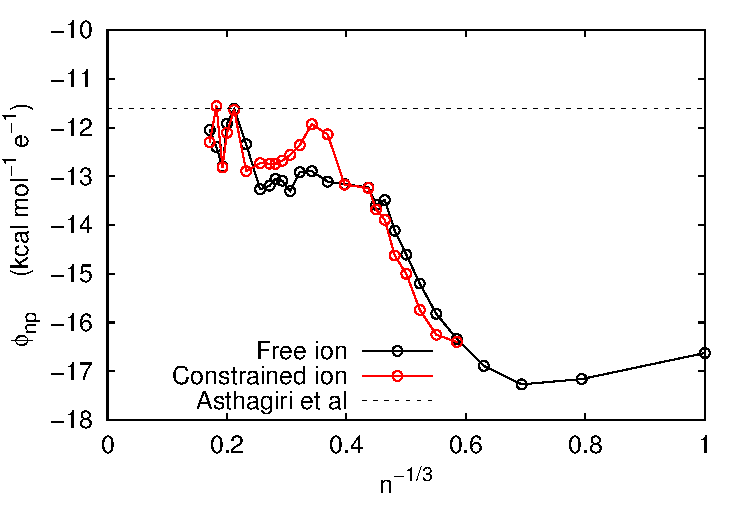
\includegraphics[width=0.98\linewidth]{images/cpa/net_pot-eps-converted-to.pdf}
 \end{center}
\caption[Net potential assuming experimental temperature derivative]{The electrochemical surface potential as a function of cluster size up to \emph{n} = 200 (using Equation 
\ref{eq:netpot2}). The temperature derivative of the net potential was assumed to be -9.9 cal/mol-K-\emph{e}, as taken from Randles\cite{randles1977structure}. The plots 
are for the cases in which the ions was either restricted to the cluster center of mass or free to move throughout the cluster. The F$^{-}$ Thole damping parameter has
been reduced from the default 0.39 value to 0.2 in generating the trajectories. The cluster size is given as n$^{-1/3}$. Error bars are comparable to or smaller than 
the size of the points (approximately $\pm$ 0.10 kcal mol$^{-1}$ or less). The dashed horizontal line is the -11.6 kcal/mol-\emph{e} value taken as an average of sign dependent
deviation in the LPS model of Ref. \cite{ashbaugh2008lps}.}
\label{fig:netpotlps}
\end{figure}

  \section{\label{ch5:sec4:level1}Discussion~}
  In conjunction with the results from Chapter \ref{ch5:sec3:level2}, my efforts suggest a proton hydration free energy of -264.7 kcal/mol, an enthalpy of -271.9 kcal/mol, an 
  entropy of -24 cal/mol-K, an electrochemical surface potential of water of -0.4 V, and a temperature derivative of the potential that is close to zero at room temperature. 
  These were revised in Ref. \cite{pollard2014cpa2} to a free energy of -264.2 kcal/mol, an enthalpy of -271.6 kcal/mol, an entropy of -24.5 cal/mol-K presented in the paper
  but not touched on here. In general, the values reported in Ref. \cite{pollard2014cpa2} should supersede those presented in Ref. \cite{pollard2014cpa1}.

  The above values differ in several respects from previous discussions and ongoing work. H\"{u}nenberger and Reif\cite{hunenberger2011sp} present an exhaustive compilation
  of proton hydration data, and based on an average of 98 values, recommend -264.8 kcal/mol for the free energy, -272.2 kcal/mol for the enthalpy, and -25 cal/mol-K for
  the entropy (labelled as \emph{intrinsic} or bulk values). While these results appear to agree well with the real values listed above, they are obtained as an
  average over data that includes both bulk and real quantities. The averaging then blurs the distinction drawn here between bulk and real quantities and its likely
  importance in determining the surface potential. The recommended real values in Ref. \cite{hunenberger2011sp} are -261.7 kcal/mol (free energy), -266.2 kcal/mol (enthalpy), 
  and -15.2 cal/mol-K, respectively, showing a large deviation from the results obtained here. 

  Ref. \cite{hunenberger2011sp} also recommends an electrochemical surface potential value of +0.13 V and a temperature derivative of -9.9 cal/mol-\emph{e} (-0.42 mV/K-\emph{e}). 
  The temperature derivative is similar to the result previously discussed by Randles\cite{randles1977structure}; from that temperature derivative, and an extrapolation to the
  critical point of water, Randles obtained a value for the electrochemical surface potential close to the +0.13 V value. Ref. \cite{hunenberger2011sp} discusses several possible
  concerns related to the previous experimental analysis of the temperature derivative. Also, it's worth mentioning that a smooth extrapolation from room temperature and 
  atmospheric pressure to the critical point is not likely a justified route for obtaining the net potential. 

  In a recent theoretical study aimed at examining the role of dispersion in ion solvation,\cite{duignan2013continuum2} the surface potential value recommended by H\"{u}nenberger
  and Reif\cite{hunenberger2011sp} was used, and it was argued that the CPA values such as those in Refs. \cite{coe1998cpa1} and \cite{donald2010expand_cpa} are bulk (or intrinsic)
  values that include no surface potential contribution. Previous simulations of large clusters, however, have been shown to include a surface potential 
  contribution\cite{beck2013sp,pollard2014cpa1}. The agreement of the computed (large cluster) results with the modified CPA analysis presented here (that is free of 
  extra-thermodynamic assumptions) provides clear evidence that the CPA-derived values correspond to the real quantities and not the bulk quantities. My results for the net
  potential rely on the assumption that the Marcus values are the bulk quantities, however. The main evidence in favor of this interpretation is the agreement between the 
  Marcus\cite{marcus1985book} and LPS\cite{ashbaugh2008lps} scales (after adjusting for the -11.6 kcal/mol potential).

  Finally, recent simulation studies of the electrostatic potential at the center of neutral cavities in water implies a value close to zero for the net 
  potential\cite{baer2012electrochemical,remsing2014lp}. In this work, the cavity was created by providing a repulsive force on the water oxygens. A previous study\cite{shi2013length} 
  showed, however, that the potential can change significantly if repulsions are included (in classical models) on the water hydrogens. An interesting alternative would be to 
  strictly enforce the cavity by excluding all electron density.

  \section{\label{ch5:sec5:level1}Conclusions~}
  The present chapter thus provides a contrasting view of proton hydration and the water surface potential. I have approached the problem from an alternative 
  thermodynamic direction that does not rely on direct electrostatic calculation of the net potential but rather infers its value by comparing ion enthalpy differences
  in large clusters with tabulated bulk values. Due to the relatively rapid convergence with cluster size of the enthalpy differences for the NaF kosmotropic pair (in
  the range \emph{n} = 10--20), it is hoped that experimental results on clusters in this size range may provide a test of the theoretical proposals outlined here.
  
  Additionally, this work has independently derived a single-ion thermodynamic scale when combined with the conventional (relative to H\sur{+}) thermodynamic scale.
  This scale defines real hydration properties which differ from the bulk values by inclusion of the net potential I reviewed previously. This scale differs somewhat 
  from the CPA scale of Tissandier et al.\cite{coe1998cpa1} and a separate recently derived scale of Vlcek et al.\cite{vlcek2013cpa} but is similar to that described 
  by Zhan et al.\cite{zhan2001absolute}. I would recommend that additional work to resolve the issues with the temperature derivative be performed. These calculations
  are planned using the Tinker package\cite{ponder2004tinker} and the iAMOEBA (improved AMOEBA) model which performs well for a number of properties over a broad 
  temperature and pressure range. A model equation of state will be useful in directing targeted simulations with greater accuracy with \emph{ab initio} molecular dynamics.

\end{cpa} % cpa papers
 \begin{tatb}
 \chapter{Revisiting the TA+/TB- hypothesis: interfacial potentials in periodic boundaries~}
 \hyperlink{toc}{Return to TOC}
  \section{\label{ch6:sec0:level1}Preface~}
  
   Disclaimer: this chapter is subject to additional changes as it is not yet published.
  
   The free energy change for transferring an ion across chemical interfaces includes a surface potential contribution. This potential has two parts: 1) the actual 
   surface or contact potential between two immiscible phases and 2) a solvent-specific local potential around the ion. In periodic boundary calculations without 
   an explicit vapor or vacuum region, the second potential still contributes to the solvation free energy and enthalpy. Simulation results therefore fall on an 
   unphysical, intermediate thermodynamic scale which needs to be adjusted to remove 2) or add 1) in order to properly facilitate comparison with one of the two
   major branches of single-ion quantities. Using ionic parameters which have not been optimized to fit one of these scales and which approach the size limit of the 
   tetraphenylarsonium and tetraphenylborate ions, I illustrate that the intermediate free energy scale is the one which predicts the $\approx$20 kcal/mol hydration
   asymmetry in water\cite{wipff1999tatb,wipff2000tatb,wipff2001tatb}. These large ions are otherwise assumed to have the same solvation free energy due to ample 
   charge screening effects\cite{marcus1987tatb}. The bulk or \emph{intrinsic} free energy scale (removing 2) above) predicts a 2-4 kcal/mol deviation from this 
   ideal behavior. I have also made predictions of the deviation in dimethyl sulfoxide and 1,2-dichloroethane, covering a broad spectrum of dielectric constants
   (10 to 80). I find dimethyl sulfoxide satisfies this condition as well while 1,2-dichloroethane violates it thanks to a large, anion favoring asymmetry. My 
   results in water and dimethyl sulfoxide compare favorably against another theoretical assessment which also falls on the bulk free energy scale\cite{pliego2015ccqct}. 
   This study builds on the emerging narrative that surface effects can differ substantially from the bulk and also has important implications in the force field 
   development community.
   
   Single-ion solvation free energies were calculated using the quasichemical theory to spatially resolve the free energy, dividing the solvation process into 3 
   distinct contributions: 1) a packing term related to cavity formation in the pure solvent, 2) an inner shell term related to the ion specific work necessary to 
   dig the same size cavity around the ion, and 3) long-range solvation effects not captured in the inner shell term. In Chapter \ref{ch1:sec1:level2} I said,
   
   \vspace{12pt}
   
   ``The desired theoretical model should take care to accommodate the major contributions to the free energy change, 1) interaction part between the ion and solvent as
     well as 2) a change in the free energy associated with the reorganization of solvent molecules around the ion (cavity formation). The interaction part can be split 
     up into 1a) local effects arising from the strong $\approx$ 1 V/\AA~fields around the ions\cite{sellner2013ionfield} and 1b) distant solvation effects which may be 
     amenable to computationally inexpensive approximations in dilute conditions, and 1c) interactions with a distant surface or chemical interface.''
     
   \vspace{12pt}
   
   \noindent It is seen that the quasichemical theory addresses each of these contributions, though it is not immediately obvious where the interfacial potentials
   come into play. Consider that the outer shell contribution can be split into vdW and electrostatic components via a cumulant expansion as illustrated below,

   \begin{equation}
    \begin{aligned}
     \beta\mu\sursous{ex}{os} &= \mu\sursous{ex}{os, vdW} + \mu\sursous{ex}{os, elst} \\
                              &= \mu\sursous{ex}{os, vdW} + q\left<\phi\sous{lp}\right>_{M(\lambda)}
                                 - \frac{\beta q\sur{2}}{2}\left(\left<\phi\sursous{2}{lp}\right>_{M(\lambda)}
                                 - \frac{\xi}{\beta L}\right)
                                 + \frac{\beta\sur{2}q\sur{3}}{6}\left<\phi\sursous{3}{lp}\right>_{M(\lambda)} + \dots
     \label{eqn:os}
    \end{aligned}
   \end{equation}

   \noindent where M($\lambda$) refers to sampling configurations with an external cavitation potential included as discussed in Chapter \ref{ch2:sec4:level4:zone2}.
   A cumulant expansion of the electrostatic part of the outer shell free energy generates a mean-field, quadratic, cubic, and higher order terms (though I truncate this 
   series to third order). The quadratic term depends on the square of the ion charge and fluctuations in the electrostatic potential felt by the ion, with the other part
   here representing a self-energy correction. This form also resembles the Born solvation model discussed in Chapter \ref{ch1:sec2:level2} and has been shown to be 
   accurate for the description of long-range interactions\cite{beck2011local,beck2011lmft,hummer1996,shi2013length}. The first and third order terms exhibit a sign
   dependence and are summed together to give the local potential. 
   
   The free energy is measured using a mid-point approximation discussed below and the local potential by accumulating statistics of the electrostatic potential at the 
   center of a large, uncharged cavity over the course of a simulation. There are several deficiencies associated with this method, but it is likely accurate for cavities 
   of $\ge$0.9 nm radius where Ashbaugh shows the potential converges in water\cite{ashbaugh2008lps}. This distance is assumed to be a reasonable length scale in the other
   solvents as well. At any rate, differences in $\mu\sursous{ex}{os,elst}$ across the range of ions considered are nearly zero for each of the solvents. The result is 
   certainly less ambiguous in the non-aqueous solvents given the fact that hydrogens in these molecules have non-zero Lennard-Jones parameters in the force field used 
   (OPLS/AA).

   This section addresses three of the questions I posed in Chapter \ref{ch1:sec1:level4},
   
   \begin{itemize}
       \item Do chemical interfaces contribute to single-ion thermodynamics? 
       \item If so, what is the contribution?
       \item How can we compare our simulation results to experiment?
   \end{itemize}

  \section{\label{ch6:sec1:levelx}Solvation free energies from the TA\sur{+}/TB\sur{-} assumption~}
   The TA\sur{+}/TB\sur{-} hypothesis and its variants (e.g., replacing TA\sur{+} with tetraphenylphosphonium) represents one of the most widely used extrathermodynamic
   assumptions used to tease apart individual ion hydration free energies, enthalpies, entropies, partial molar heat capacities, equivalent conductivities, and Dole-Jones
   B-coefficients\cite{marcus1987tatb}. Marcus speaks highly of the method, remarking that it has found support over the years and is generally regarded as the 
   ``least objectionable'' of the myriad extrathermodynamic assumptions\cite{marcus2015book}. In a field rife with complex thermodynamic cycles and often suspect 
   assumptions, TA\sur{+}/TB\sur{-} is also without doubt one of the simplest models relying only on the disappearance of ion-specificity when incorporating a pair of 
   oppositely charged ions into a large molecular framework to isolate it from the solvent. The hypothesis is not entirely without issue, however, as the molecular ion
   pair exhibit a small inequality in their vdW radius leading to a 1.2\% error in electrostatic interactions and 2.2\% in the solvation energy of the neutral 
   particle\cite{kim1978tatb, marcus2015book}.

   The method provides a means to easily construct a universal thermodynamic scale in all solvents as the peripheral ligands always mask the identity of the charge. 
   Solubility or electrochemical measurements are used to measure free energies of transfer from water, W, to another solvent, S, with an accuracy argued to be on the 
   order of $\pm$ 2 kJ/mol\cite{marcus2015book}. Measurements of the W$\rightarrow$S transfer may be taken in mutually saturated solvents that are in contact with one 
   another or in the pure solvent. The choice can often lead to very different results as the more hydrophilic ions tend to coextract with residual waters into the 
   non-aqueous phase\cite{rose2009, darvas2011, darvas2013}. A universal thermodynamic scale is essential to linking theoretical measurements to their experimental 
   counterparts, providing a means to accurately predict the pH of mixed electrolyte solutions used in liquid chromatography\cite{suu2015mixedpH}, measure absolute 
   electrochemical potentials and convert to non-aqueous solvents (in both theory and experiment)\cite{isse2010univscale}, and in the development of force fields for 
   molecular simulation.

   There is however evidence of sign specific effects on water structure around the ions which suggest anions are more strongly hydrated than cations. Several of these
   evidences are visited by Grossfield et al. (see the bottom left column on page 2)\cite{ren2003amoebaion}. These observations are primarily 
   spectroscopic in nature. I also find that approaching the TA\sur{+}/TB\sur{-} limit, anions are better solvated in water and 1,2-DCE and cations in DMSO. However, 
   the asymmetry changes after modifying the simulation result to exclude the interfacial potential and reflects any true sign specificity in the solvation free energy.
   
  \section{\label{ch6:sec1:level1}Computational methods~}
   All calculations in this Chapter were performed in double-precision with Gromacs 4.6.7\cite{gromacs} installed locally on the Oakley and Ruby clusters at the Ohio 
   Supercomputer Center\cite{osc}. The OPLS-AA\cite{opls} force field was used for DMSO and 1,2-DCE. SPC/E\cite{spce} parameters were used for water. Bonds and angles 
   involving hydrogen atoms were constrained with the LINCS algorithm\cite{lincs} in all simulations. Ions parameters are listed in Table \ref{tab:ion_labels} and range
   from 0.3 nm to 0.55 nm in radius, the same size used in the Schurhammer and Wipff studies\cite{wipff1999tatb, wipff2000tatb, wipff2001tatb}. Dispersion
   parameters were chosen to surround the Schurhammer and Wipff value of 0.42 kJ/mol with the smaller value matching that of I\sur{-} in the Horinek and Netz force 
   field\cite{netz2009}. The larger value is just an order of magnitude greater.

\begin{table}
 \begin{center}
  \begin{tabular}{ccc}
   \hline
   \hline
    Charge (Label) &   Radius   &   $\varepsilon$  \\
   \hline
    +(ak)/-(ka)    &   0.30     &    0.16          \\
    +(bl)/-(lb)    &   0.40     &    0.16          \\
    +(cm)/-(mc)    &   0.45     &    0.16          \\
    +(dn)/-(nd)    &   0.50     &    0.16          \\
    +(eo)/-(oe)    &   0.55     &    0.16          \\
    +(fp)/-(pf)    &   0.30     &    1.60          \\
    +(gq)/-(qg)    &   0.40     &    1.60          \\
    +(hr)/-(rh)    &   0.45     &    1.60          \\
    +(is)/-(si)    &   0.50     &    1.60          \\
    +(jt)/-(tj)    &   0.55     &    1.60          \\
   \hline
   \hline
  \end{tabular}
  \caption[Labels and parameters assigned to fictitious ions]{\label{tab:ion_labels}Parameters of the ions used in this study. Units are nanometers and kJ/mol. 
  Charges are $\pm$ 1. The first column ascribes a label for each ion. The anion label is merely the reverse of the binary sequence used to label the cation. These 
  pairs differ only in their charge.}
 \end{center}
\end{table}

   The Good-Hope\cite{goodhope} and Berthelot\cite{berthelot} combining rules were used to generate the pair $\sigma\sous{ij}$ and $\varepsilon\sous{ij}$ parameters, 
   respectively. The ion/cavity/solvent or cavity/solvent systems were equilibrated in the NPT ensemble for 400 ps at 1.0 bar and 298.15 K using the Berendsen 
   barostat\cite{barostat} and V-rescale algorithms\cite{vrescale} for pressure and temperature coupling. Real-space and vdW interactions were truncated at 1.2 nm,
   with a 0.16 nm grid spacing and 6\sur{th}-order spline for reciprocal space interactions. I used an Ewald convergence parameter of $\eta =$ 5.6/L where L is the box
   length after NPT equilibration. Energies were sampled every 20 frames from 2.0 ns of a 2.2 ns production run in the NVT ensemble, also held at 298.15 K with the
   V-rescale algorithm\cite{vrescale}. For quantities obtained through thermodynamic integration, 21 unique $\lambda$ values were used. Each simulation, including at 
   each $\lambda$, was performed 3 separate times with a timestep of 2.0 fs. Statistical errors were evaluated with the block-averaging method; errors were propagated
   through numerical integration as well. The solvation environment around an ion with the fully grown cavity in each solvent is illustrated in Figure
   \ref{fig:expelled_volume}. The cavity had a 0.9 nm radius and did not change with ion size. This leads to decreasing inner shell contributions with increasing 
   ion size and increasing outer shell contributions through the vdW potential.

   The solvents modeled here cover a broad range of dielectric constants from 10 to 80. For additional validation of the methods used here I also computed dielectric
   constant for each solvent. I performed 400 ps of equilibration of the pure solvent without cavities as above followed by 10 ns constant volume dynamics at 298.15 K.
   The first 500 ps of each trajectory was discarded as additional equilibration. The SPC/E dielectric constant was found to be 72 (71), in DMSO it was 45 (42), and in
   1,2-DCE it was 12 (13). Values in parentheses were taken from Reddy et al.\cite{reddy1989dielectric} and Caleman et al.\cite{caleman2011force}. I also performed
   this study with acetonitrile but the OPLS/AA force field produced a dielectric of 20 which is about half that of the experimental value and so performed very
   poorly\cite{caleman2011force}.

\begin{figure}
 \begin{center}
  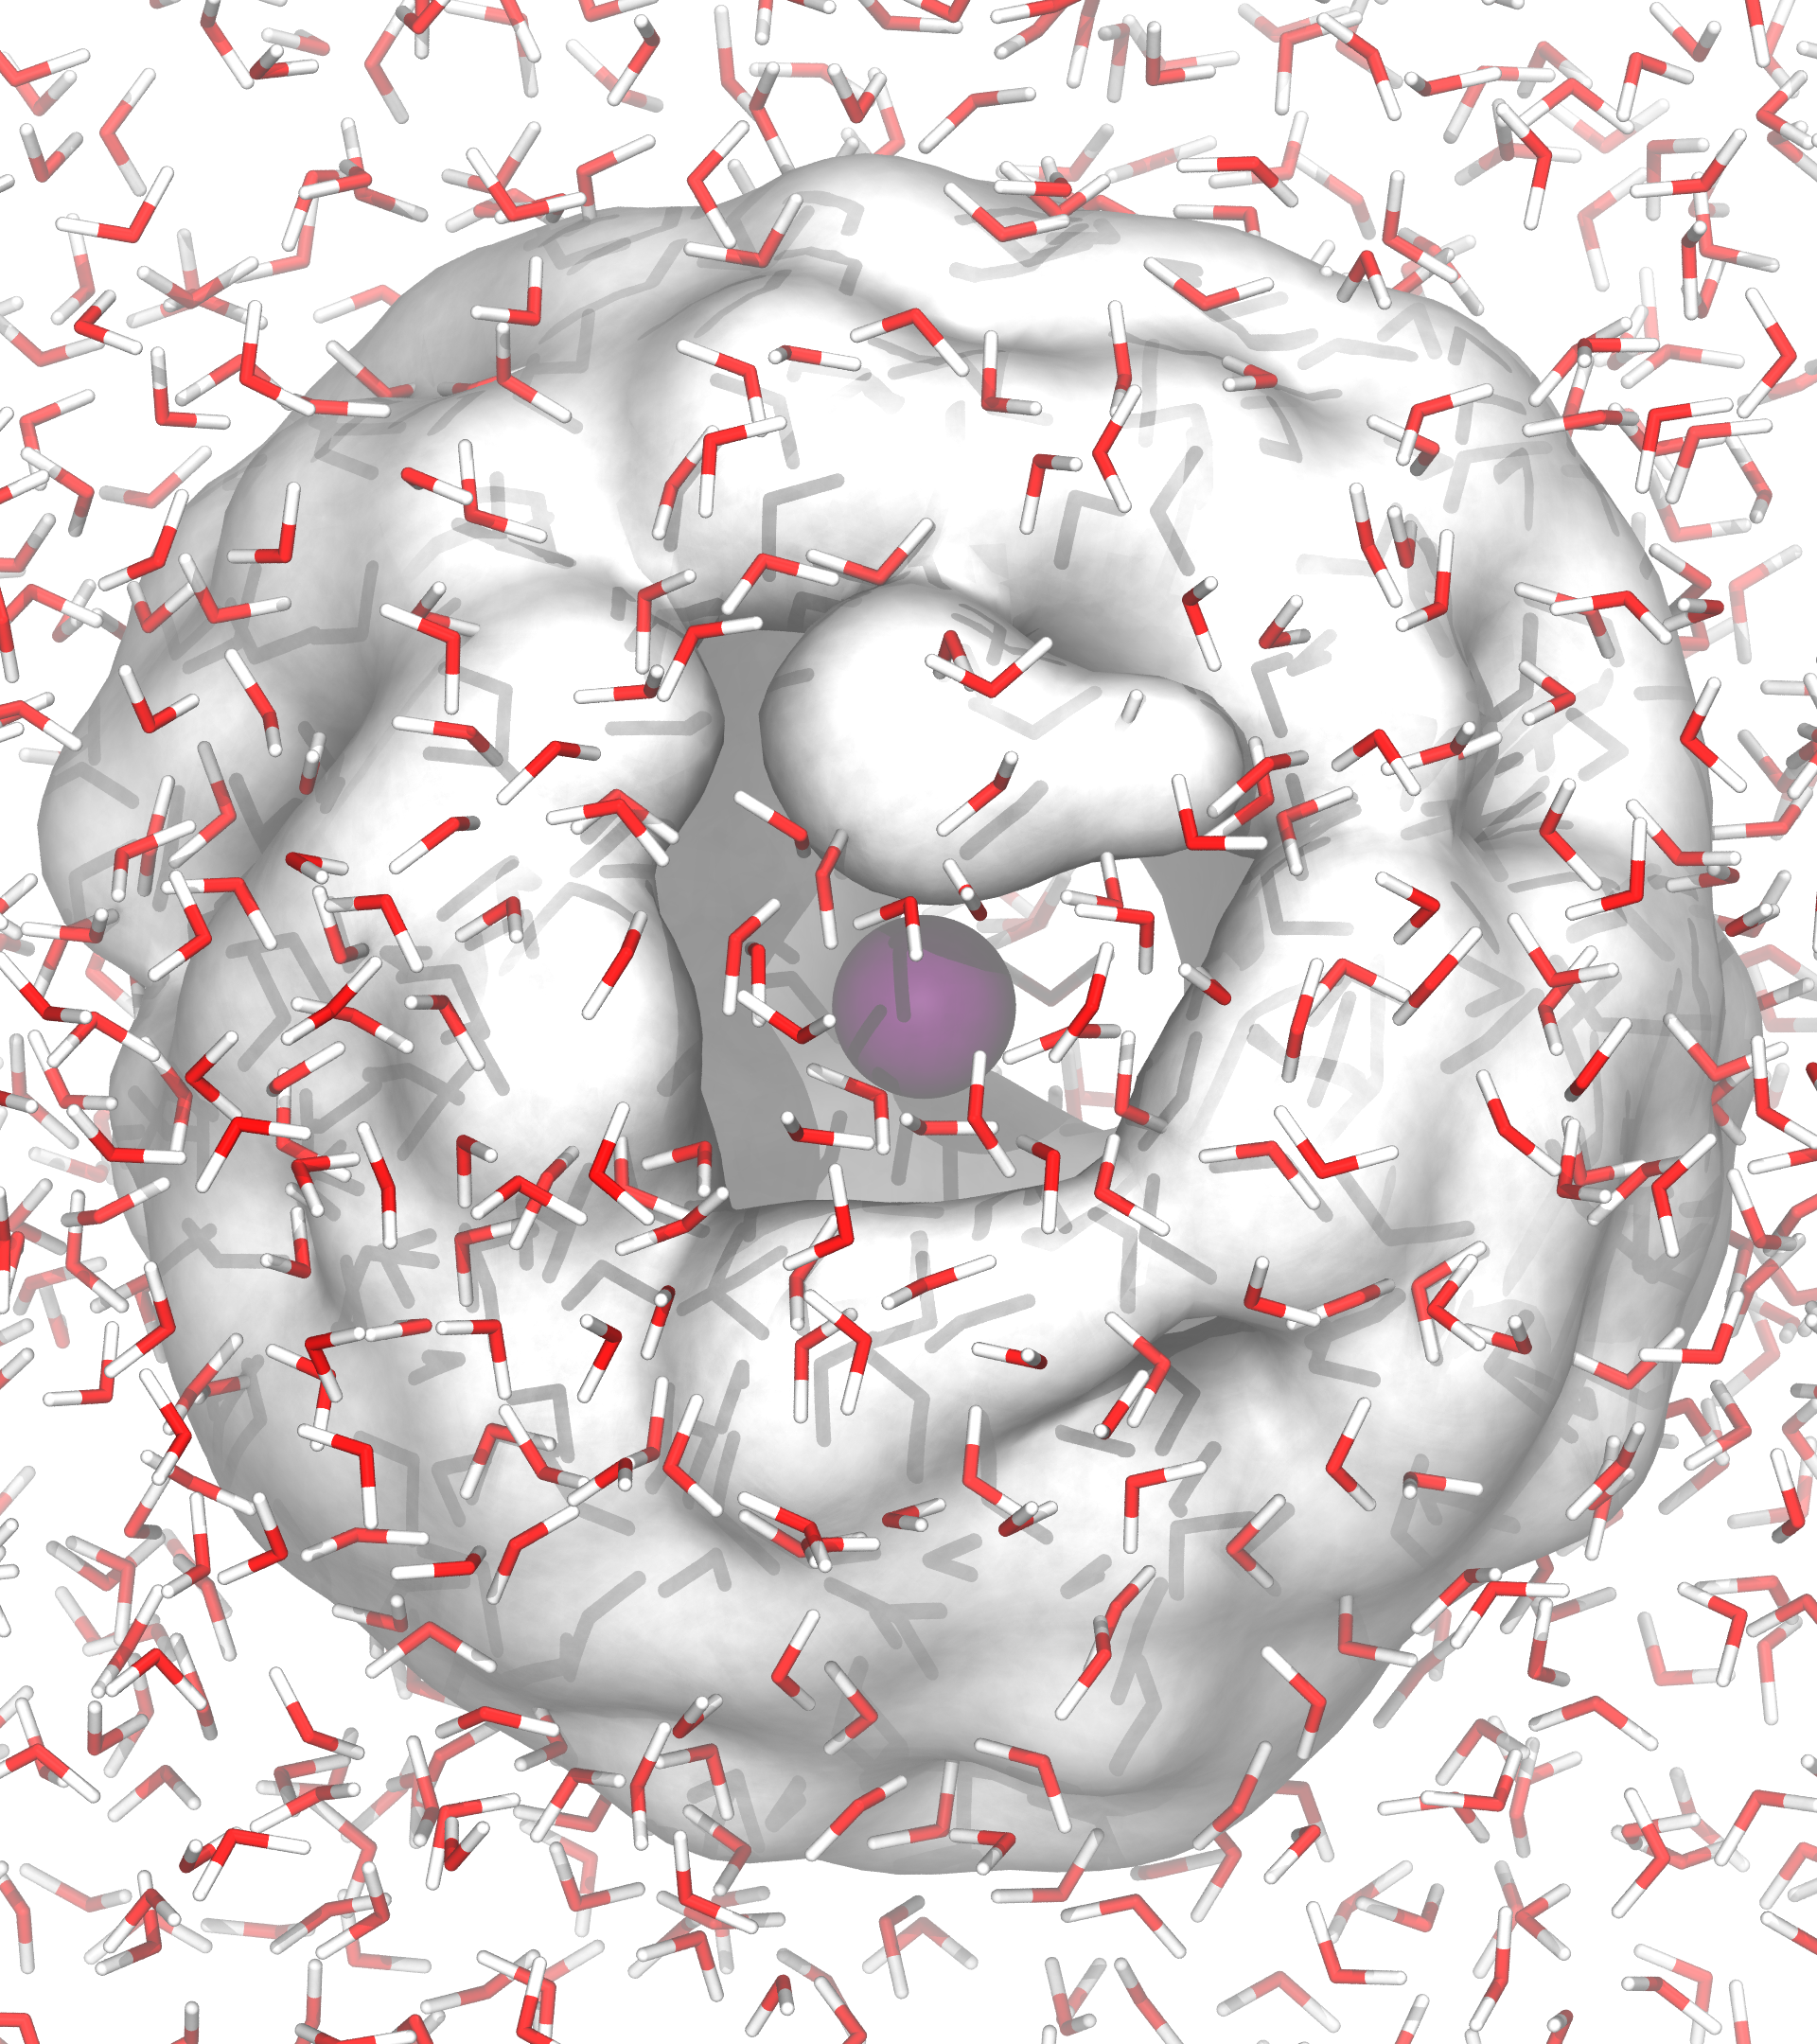
\includegraphics[width=0.30\linewidth]{images/tatb/wat.png}
  \includegraphics[width=0.30\linewidth]{images/tatb/dmso.png}
  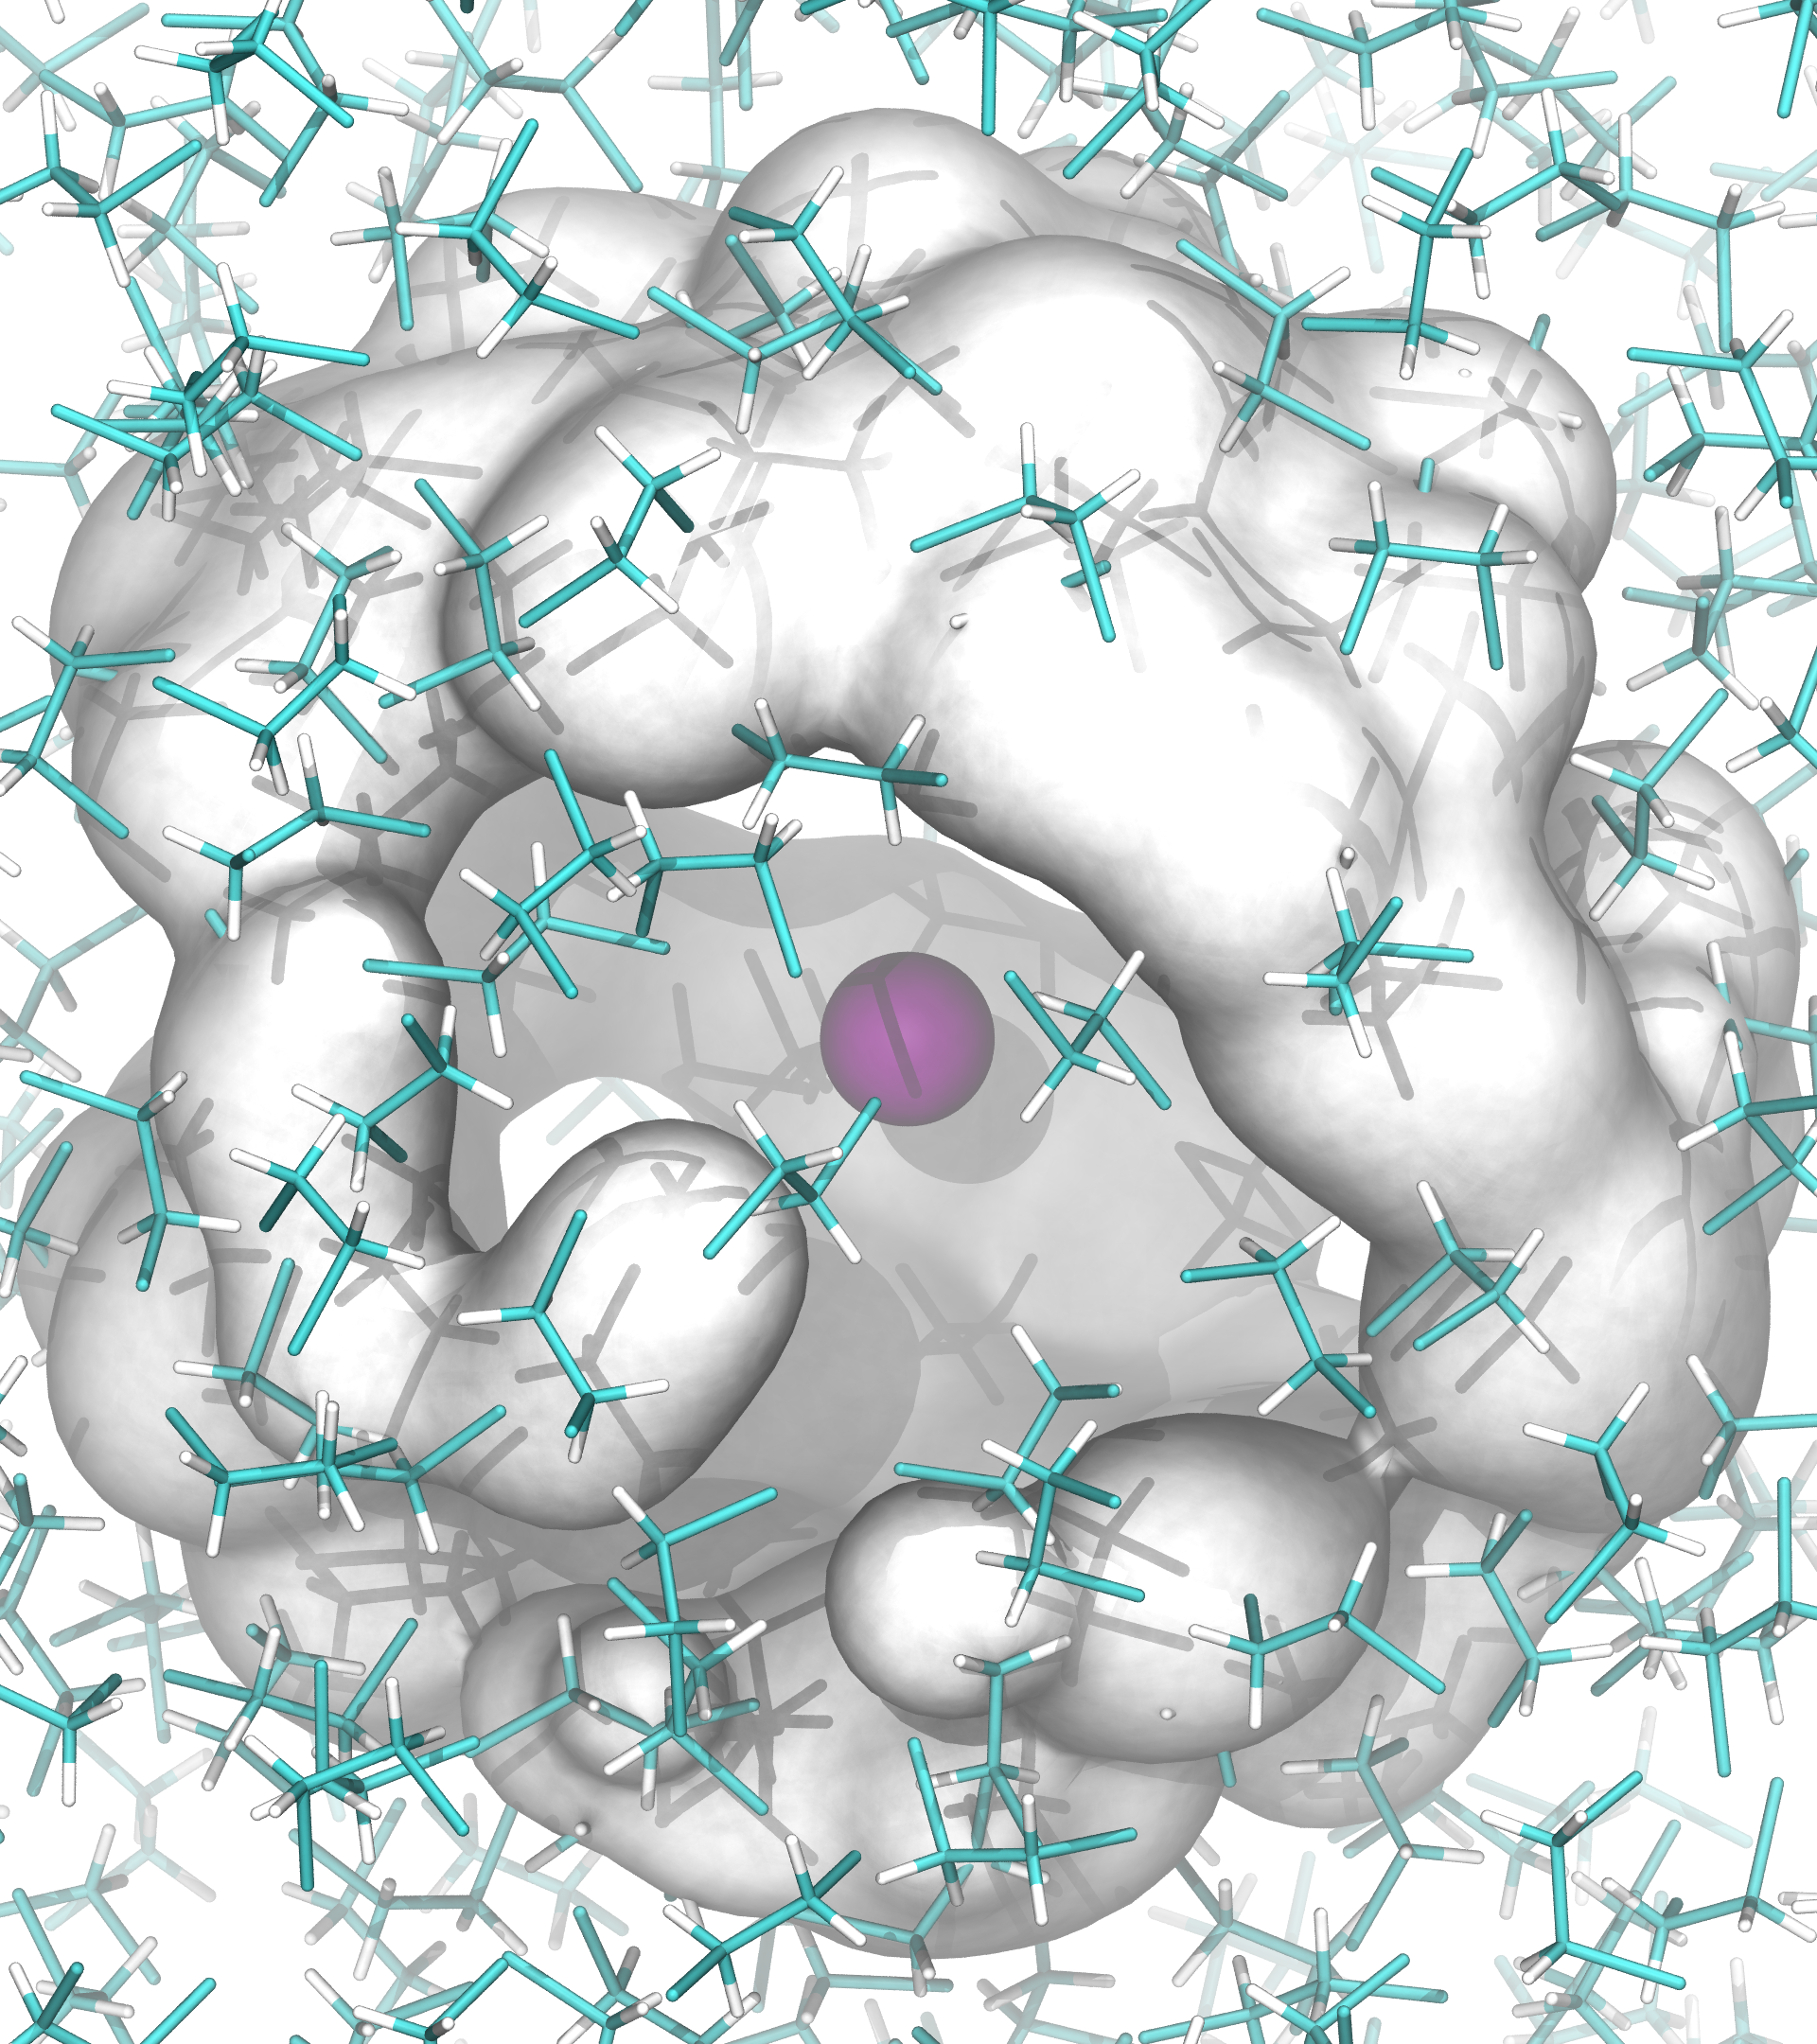
\includegraphics[width=0.30\linewidth]{images/tatb/dce.png}
  \caption[Snapshots of solvents with cavity volume excluded]{\label{fig:expelled_volume}Visualization of solvation structure at the boundary (white surface) 
  of the 0.90 nm radius cavity used to compute solvation free energies. The ion is at the center of this void, and is shown in purple. The solvents from left to 
  right are as follows: water, dimethyl sulfoxide, and 1,2-dichloroethane.}
 \end{center}
\end{figure}
 
  \section{\label{ch6:sec2:level1}Results~}

  \subsection{\label{ch6:sec2:level2}Packing and inner shell terms}
  I begin with some discussion of the cavity-related terms in each solvent: the packing and inner shell contributions. The packing free energy is independent of the 
  ion so I can very simply list the values for each solvent. For water this came out to 82.77 $\pm$ 0.63 kcal/mol which compares favorably with the result from Shi and
  Beck who produced a fit to a scaled-particle theory model\cite{shi2013length}. This value reflects the work required to clear a void of only the water oxygens since
  the hydrogens do not participate in the vdW potential. However, for both DMSO and 1,2-DCE, the hydrogens in these molecules have been assigned non-zero $\sigma$
  and $\varepsilon$ parameters. The cavity potential I used made no distinction between this atom or that based on mass and so acted the same on all particles provided 
  the force field recommended non-zero vdW parameters. A slightly larger value of 83.50 $\pm$ 0.91 kcal/mol was obtained for DMSO, while a much smaller result of 49.45
  $\pm$ 0.56 kcal/mol was found for 1,2-DCE. It's interesting to note that the cavity formation free energy in DMSO remains so large in spite of the pair of methyl 
  groups the solvent is forced to accommodate. Solvent/solvent contacts in 1,2-DCE however do appear to be relatively weak compared to both water and DMSO. Consequently, 
  the solvent is less tightly packed and so offers substantially less resistance to the insertion of large cavities and likewise to large, hydrophobic molecules and ions. 
  You can get a sense of this visually from Figure \ref{fig:expelled_volume} as well.

  A connection between the quasichemical packing contribution and the surface tension of the solvent was developed in Ref. \cite{shi2013length}. The surface tension for
  OPLS 1,2-DCE is 23.2 mN/m (expt 31.86 mN/m) while OPLS DMSO matches the experimental figure of 42.92 mN/m remarkably well (calc 42.4 mN/m)\cite{caleman2011force}. 
  Like 1,2-DCE, the surface tension of the SPC/E model (63.6 mN/m) is somewhat smaller than the experimental value (71.73 mN/m)\cite{vega2007surface}. Based on the model
  of Shi and Beck, I should still expect to see the packing contribution of water to be larger than DMSO, despite the smaller than expected SPC/E water surface tension.
  However, my finding is consistent with a scaled particle theory estimate from Abraham et al.\cite{abraham1979use}. Assuming the cavity term in Ref. \cite{abraham1979use}
  is positive too, then pack(DMSO) - pack(water) $>$ 0 means it costs more energy to put the cavity (here the cavity has a diameter of 0.84 nm) into DMSO. Their model
  appears to take into account the size of the solvent particles, which may account for the unexpected result.

  I continue the discussion focusing on Figure \ref{fig:inner}. For all ion $\sigma$ and $\varepsilon$ considered, the chemical part of the free energy showed that 
  the anion was better solvated in water and 1,2-DCE than the cation and generally followed the opposite trend in DMSO due to the hard S$=$O moiety. The gap between the 
  $\mu$\sursous{ex}{is} of complementary ions pairs (oppositely charged pairs with all other properties equal) diminishes to nearly zero for the largest radii in DMSO and
  water. This appeared to not be the case for ion solvation in 1,2-DCE where the charge-specific differences in smaller ion pairs remained essentially constant even when I 
  simulated TA\sur{+}/TB\sur{-}-sized particles. These results shed an initial favorable light on the validity of the TA\sur{+}/TB\sur{-} assumption in water and in DMSO as
  the large ions share nearly identical free energies in the ion specific region. A small amount of ion specificity is expected to survive based on the finite-size corrected
  fluctuation contributions in Figure \ref{fig:fq_flucts} which still show preference for one ion over the other, even using ions of TA\sur{+}/TB\sur{-} size. This hints 
  that the validity of the TA\sur{+}/TB\sur{-} assumption may rely on cancellation of lingering ion specificity by the $\phi$\sous{lp}.
  
\begin{figure} 
 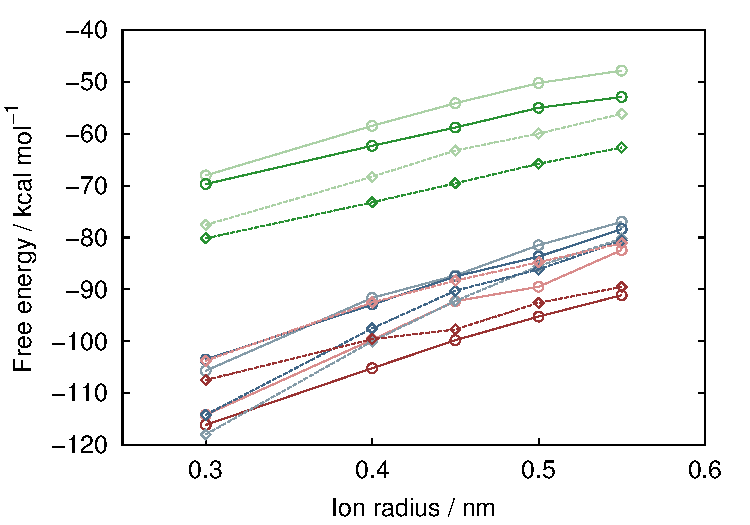
\includegraphics[width=0.98\linewidth]{images/tatb/is.pdf}
 \caption[Inner shell (chemical) part of the solvation free energy]{\label{fig:inner}Chemical or inner shell part of the solvation free energy for the ions in water
 (blues), dimethyl sulfoxide (reds), and 1,2-dichloroethane (greens). The darker shade corresponds to ions with $\varepsilon =$ 1.60 kJ/mol and the lighter shade for
 $\varepsilon =$ 0.16 kJ/mol. The cations are presented here with open circles at the sampled radii linked together with a solid line; anions at the sampled radii are
 represented as diamonds and are joined together with dashed lines. Error bars are omitted as they are about the same size as the symbols and are reported in the tables
 in Appendix \ref{chap:a6}.}
\end{figure}

\begin{figure} 
 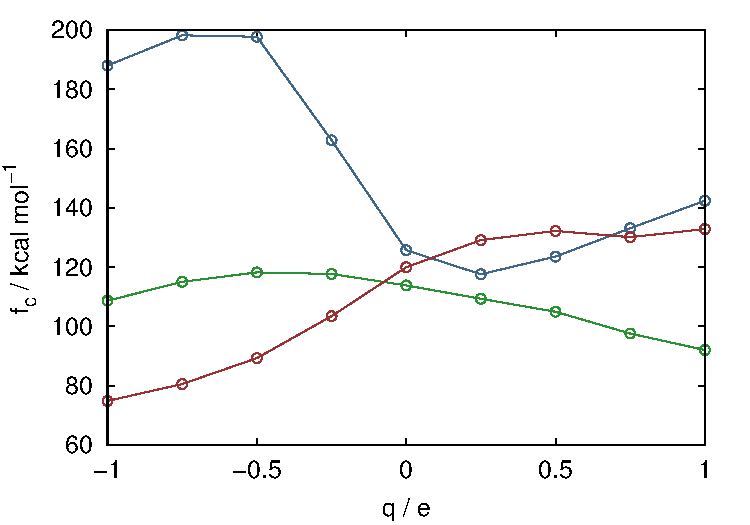
\includegraphics[width=0.80\linewidth]{images/tatb/cl_sized_fq_var.pdf} \\
 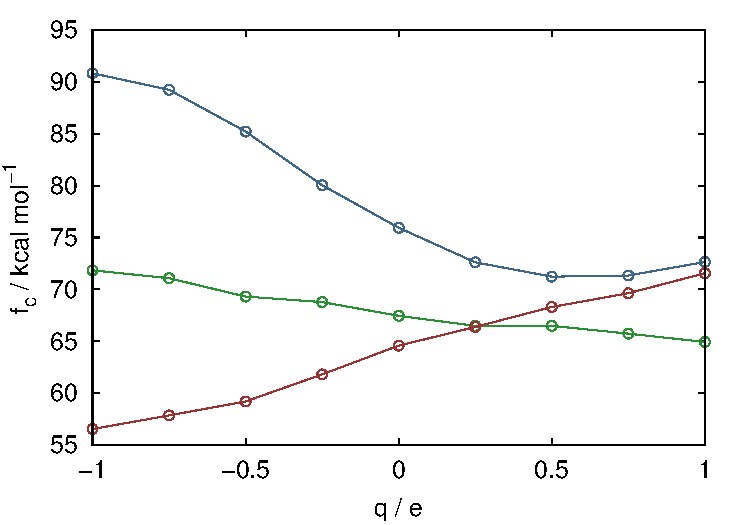
\includegraphics[width=0.80\linewidth]{images/tatb/tatb_sized_fq_var.pdf} 
 \caption[Corrected fluctuations of the electrostatic potential at the center of an uncharged cavity]{\label{fig:fq_flucts}Finite-size corrected fluctuations of
 the electrostatic potential at the center of the Horinek and Netz Cl\sur{-}-ion (top) and a TA\sur{+}/TB\sur{-}-ion (bottom). Figures are reported as solid lines 
 in blue for water, red for DMSO, and green for 1,2-DCE.}
\end{figure}

  \subsection{\label{ch6:sec2:level3}Outer shell and local potential terms}
  I begin this section with some discussion of the motivations for electing to use the mid-point approximation to the outer shell free energy. Normally, I would sample
  the fully coupled interaction energies from the final $\lambda$ state in both the packing (uncoupled) and inner shell (coupled) trajectories. However, as pointed out
  by Shi and Beck\cite{shi2013length}, there needs to be continuity in the solvation environment between that sampled with $\pm$q and a neutral but otherwise identical
  particle. Monitoring the mean-field part of the electrostatic potential at the center of a cavity bearing integer and fractional charges in the range of -q to q is a
  particularly useful way for interrogating the solvation shell for charge-specific asymmetries, see Figure \ref{fig:fq_means}. As noted by Wipff et al., the water dipole
  orientation around the
  neutral cavity more resembles the solvation environment around a positively charged ion\cite{wipff1999tatb}. Unsurprisingly, I found the mean-field part of the
  electrostatic potential for the neutral particle fell on the same line drawn through the points with positive charge. The same observation was made from the
  TA\sur{+}/TB\sur{-}-sized ion data set as well. Lines through the negatively and positively charged ion data intersect at -0.22e and -0.17e for the smaller and larger
  ion sizes, respectively. The deviation between these lines is reduced with the larger particles, but not enough to allay concerns over errors introduced by sampling
  energies from dissimilar solvation environments. I've found likewise in DMSO as well, where the lines intersect at -0.16e and -0.11e. In contrast, the solvation
  environment around the neutral cavity in 1,2-DCE slightly favored the anion and produced intersections at 0.22e and 0.03e. An additional point, the potential at the
  center of the neutral cavity can be taken as a crude estimate of $\phi$\sous{lp}, with some caveats discussed below.
  
\begin{figure}
 \begin{center}
  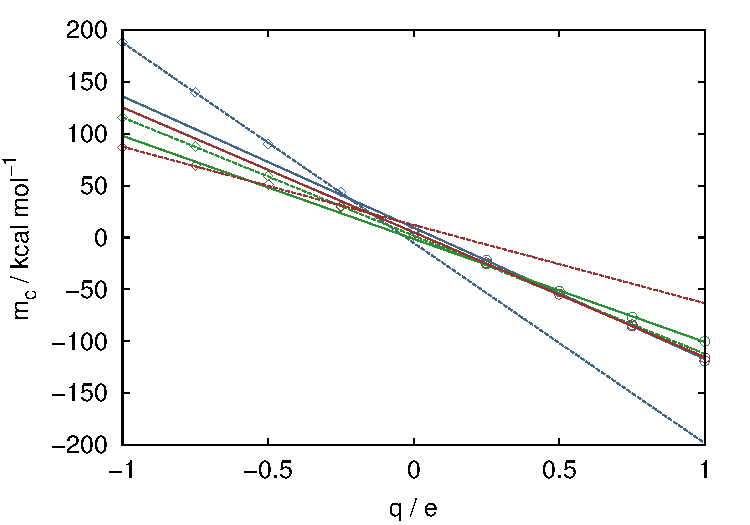
\includegraphics[width=0.80\linewidth]{images/tatb/cl_sized_fq_means.pdf} \\
  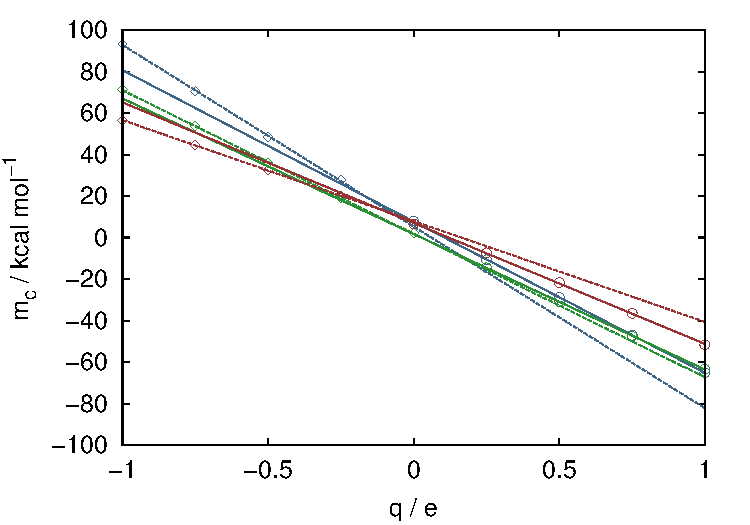
\includegraphics[width=0.80\linewidth]{images/tatb/tatb_sized_fq_means.pdf}
  \caption[Corrected mean of the electrostatic at the center of an uncharged cavity]{\label{fig:fq_means}Finite-size corrected means of the electrostatic
  potential at the center of the Horinek and Netz Cl\sur{-}-ion (top) and a TA\sur{+}/TB\sur{-}-ion (bottom). Colors correspond to solvents: blue for water, red for
  DMSO, and green for 1,2-DCE. A dashed line is used to show the linear fit through the negatively charged points and a solid line for the fit through the neutral and
  positively charged data points.}
 \end{center}
\end{figure}

  The mid-point approximation for $\mu$\sursous{ex}{os} provides a straightforward decomposition pathway to separate vdW and electrostatic sources as in Equation 
  \ref{eqn:os}. Assuming any differences in the vdW energy between the ions to be small, the top plot in Figure \ref{fig:outer} depicts the results from the cumulant
  expansion of the electrostatic contributions to $\mu$\sursous{ex}{os}. Across the range of ion radii covered here and in all solvents, this plot shows a very nearly
  constant gap between the complementary sets of ions. I argue this gap is due to the presence of a q$\phi$\sous{lp} factor for each ion. As the bottom plot in 
  Figure \ref{fig:outer} illustrates, the removal of this factor shifts the free energy differences into near perfect overlap with some residual due to non-Gaussian
  behavior in the vdW contributions for the organic solvents. The electrostatic contributions are within 0.5 kcal/mol of each other across 3 separate trajectories
  with small differences in the variance and higher order terms. A slightly larger cavity may be needed for DMSO and 1,2-DCE to remove the remaining small, but not 
  insignificant non-Gaussian behavior.

\begin{figure}
 \begin{center}
  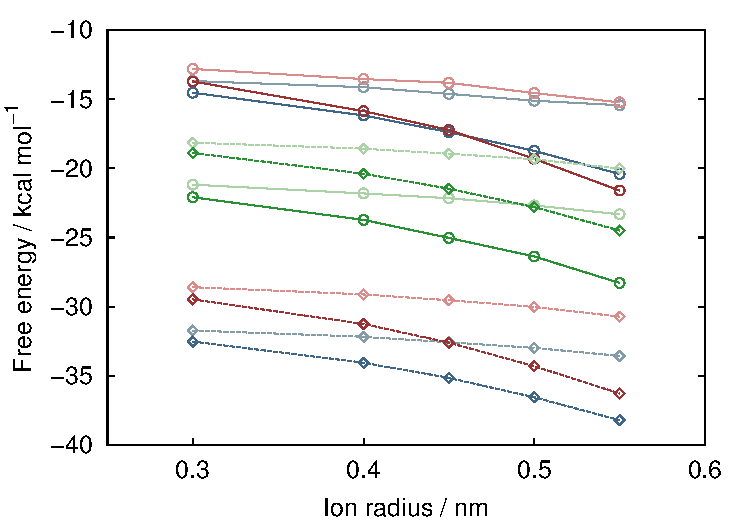
\includegraphics[width=0.80\linewidth]{images/tatb/os.pdf}
  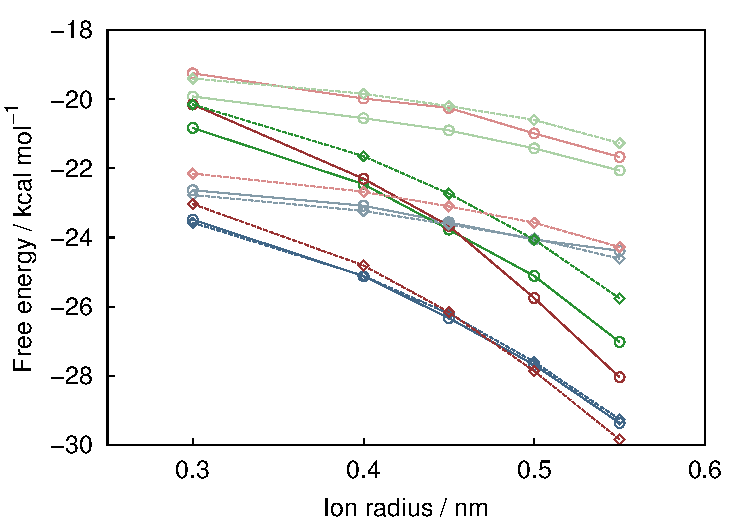
\includegraphics[width=0.80\linewidth]{images/tatb/os_m_qlp.pdf}
  \caption[Outer shell portion of the solvation free energy]{\label{fig:outer}Full outer shell (top) and outer shell less the local potential (bottom) part of the
  solvation free energy. Color and labeling scheme are the same as described in Figure \ref{fig:inner}.}
 \end{center}
\end{figure}

  The local potential in each solvent [in (mean + third cumulant); total $\pm$ error format] was determined to be (8.76 + 0.20); 8.95 $\pm$ 0.14 kcal/mol-e, 
  (6.71 + -0.27); 6.44 $\pm$ 0.24 kcal/mol-e, and (-1.42 + 0.16); -1.26 $\pm$ 0.20 kcal/mol-e in water, DMSO, and 1,2-DCE respectively. These potentials were sampled
  from configurations generated with an empty 0.9 nm radius cavity buried in each solvent. The potential makes no distinction between light and heavy atoms so long as
  they are described with non-zero terms in the conventional LJ function, else those atoms are ignored for consistency with the force field. This method was shown by
  Ashbaugh to produce well-converged results at the same length scale I used here\cite{ashbaugh2000size_sp}. Simply using the neutral point in the fluctuating 
  electrostatic potential calculations discussed previously can, in some cases, net you a fortuitously close result, but it displays significant size variance and may
  even predict the wrong sign for solvents with smaller $\phi$\sous{lp}. This is a consequence of using standard LJ interactions in the simulation which operate on 
  different length scales for each atom type, so smaller elements tend to settle a bit closer to the ion than they would with my modified WCA potential, for example.
  The local charge balance at the cavity is skewed in favor of the charge of these smaller elements, usually hydrogens. The positive charge on these atoms introduces an 
  artificial shift driving $\phi$\sous{lp} more positive, or negative as the case may be. A similar shift occurs when applying the cavity-growth potential to hydrogens 
  in the SPC/E or other single vdW-site water models and actually yields a $\phi$\sous{np} around -0.4 V, though this is almost assuredly coincidental\cite{beck2013sp}.

  \subsection{\label{ch6:sec2:level4}Free energy differences}
  I now have all the pieces needed to assemble the total solvation free energies and examine how the differences between the ions transition with increasing size. 
  These values are reported in Appendix \ref{chap:a6} in a tabular format complete with error bars for both the intermediate and bulk free energy scales. The 
  differences between the single-ion solvation free energies listed in those tables are depicted in Figures \ref{fig:uex_diffs1}, \ref{fig:uex_diffs2}, and 
  \ref{fig:uex_diffs3}. Where appropriate I have included figures taken from Wipff et al.\cite{wipff1999tatb} and Pliego et al.\cite{pliego2015ccqct} to highlight not
  only my agreement with these additional studies but to showcase that their respective results fall on very different thermodynamic scales and lead to very different
  conclusions. Removal of q$\phi$\sous{lp} from $\mu$\sursous{ex}{os} extinguishes the artificial stabilization of anions relative to their cation analogue in both 
  SPC/E water and OPLS/AA DMSO that produced the $\sim$20 kcal/mol disparity in TB\sur{-} versus TA\sur{+} solvation free energies reported by Schurhammer and Wipff.
  Withdrawing q$\phi$\sous{lp} from $\mu$\sursous{ex}{os} in 1,2-DCE created a slightly greater rift in the ion solvation free energies with a deviation from ideal
  behavior of about 6-10 kcal/mol in favor of the anion. This range is similar to that of acetonitrile as discussed by Pliego et al.\cite{pliego2015ccqct}.  

\begin{figure} 
 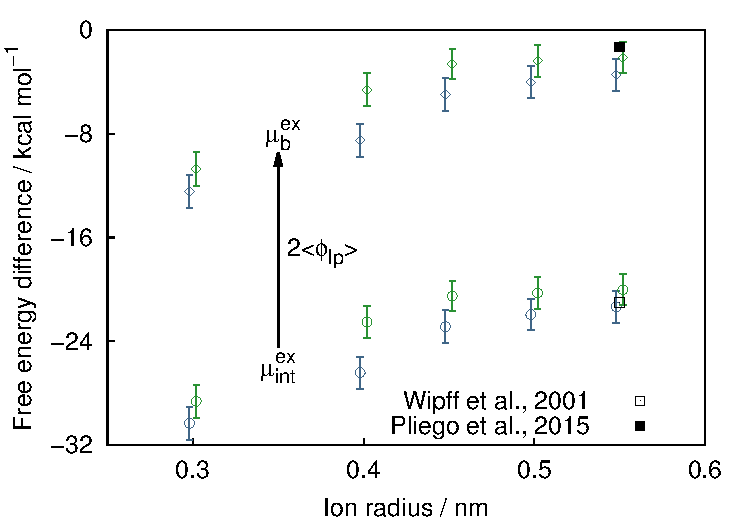
\includegraphics[width=0.98\linewidth]{images/tatb/wat_free_energy.pdf}
 \caption[Free energy differences in water]{\label{fig:uex_diffs1}Free energy differences in complimentary ion pairs in water. Open circles represent 
 intrinsic free energy points while open diamonds are on the bulk free energy scale. Blue coloring corresponds to ions with $\varepsilon =$ 0.16 kJ/mol 
 while green marks $\varepsilon =$ 1.60 kJ/mol differences. Where appropriate, comparisons to the Wipff and Pliego results are reported.}
\end{figure}

\begin{figure} 
 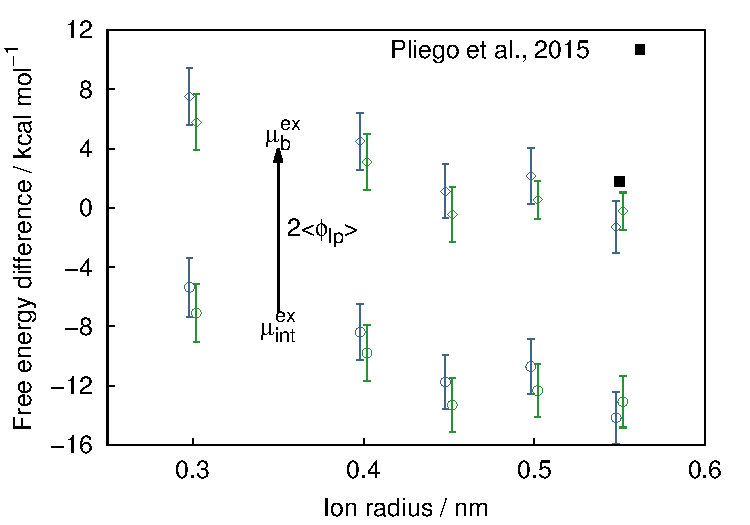
\includegraphics[width=0.98\linewidth]{images/tatb/dmso_free_energy.pdf}
 \caption[Free energy differences in dimethyl sulfoxide]{\label{fig:uex_diffs2}Free energy differences in complimentary ion pairs in DMSO. Open circles 
 represent intrinsic free energy points while open diamonds are on the bulk free energy scale. Blue coloring corresponds to ions with $\varepsilon =$ 0.16 
 kJ/mol while green marks $\varepsilon =$ 1.60 kJ/mol differences. Where appropriate, comparisons to the Wipff and Pliego results are reported.}
\end{figure}

\begin{figure} 
 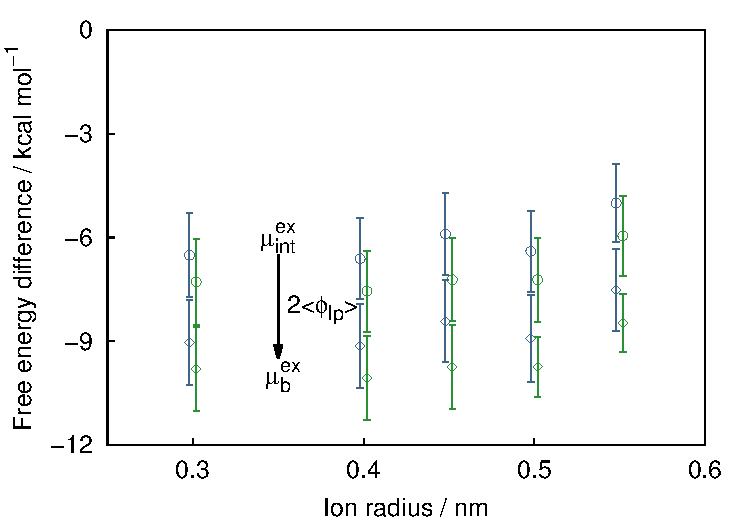
\includegraphics[width=0.98\linewidth]{images/tatb/dce_free_energy.pdf}
 \caption[Free energy differences in 1,2-dichloroethane]{\label{fig:uex_diffs3}Free energy differences in complimentary ion pairs in 1,2-DCE. Open circles 
 represent intrinsic free energy points while open diamonds are on the bulk free energy scale. Blue coloring corresponds to ions with $\varepsilon =$ 0.16 
 kJ/mol while green marks $\varepsilon =$ 1.60 kJ/mol differences.}
\end{figure}

  \section{\label{ch6:sec3:level1}Discussion~}
  Qualitatively, the result that anions are more strongly hydrated than cations falls in step with a number of other studies\cite{wipff1999tatb, pliego2015ccqct,
  ren2003amoeba, collins2007review, collins1995}. Assuming the F\sur{-} and K\sur{+} ions to be of nearly identical size (or perhaps more conservatively, between
  Na\sur{+} and K\sur{+})\cite{wright2010ionsize}, Rose et al. also concluded that the anion interacted more favorably with 1,2-DCE than the cation\cite{rose2009}. 
  And finally, in agreement with the somewhat dated conductometric studies of Exner et al.\cite{exner1974dmso} and more recent simulation results of Pliego et al. for
  intermediate\cite{pliego2002dmso} and bulk free energies\cite{pliego2015ccqct}, I found the cation produced a larger $\mu$\sur{ex} part than its complementary anion. A
  more quantitative assessment of the accuracy of my results was a bit more difficult to come by, but the extensive work of Abraham et al. (Table 8)\cite{abraham1978} 
  allowed me to get an approximate sense of where my bulk free energy results fell for the more physically motivated ion parameter sets (cations with $\varepsilon
  =$ 0.16 kJ/mol and anions with $\varepsilon =$ 1.60 kJ/mol). For example, I properly recovered that the transfer free energy from water to 
  1,2-DCE was unfavorable for smaller ions, up to the size of tetraethylammonium (TEA\sur{+}) which has an ionic radius in the neighborhood of 0.3 to 0.4 
  nm\cite{aue1976tea}. Given the trend reported in their article and second harmonic generation spectroscopic investigation of the water/1,2-DCE 
  interface\cite{conboy1997shg_tatb}, I know that larger ions eventually become better suited to the oil over water. Likewise, the cation solvation free energies in
  DMSO were found to be greater than that in water which was also observed by Pliego et al.\cite{pliego2002dmso}. For anions, the smallest one gave a positive transfer 
  free from water to DMSO consistent with these other authors but beyond that reverses. Within the limitations of the force field, these results compare rather favorably
  against other studies, but it is important to note the parameters used here were not designed to handle ion solvation problems. They neglect or oversimplify difficult
  to characterize polarization and partial charge transfer contributions\cite{pollard2016review}, which can be difficult to overcome even when fitting some of the parameters
  to high level electronic structure calculations\cite{ayse2016ecpc}. Above all though, this exercise is meant to be illustrative of a broader concern and even the
  poorest force fields are susceptible to these interfacial potential issues.

  In Table 4 of the Wipff manuscript for the spherical S\sur{+} and S\sur{-}, the authors show that the electrostatic part of the interaction energy favors the anion
  by 23 kcal/mol\cite{wipff2000tatb}. This difference is also reflected in Table 5, where they report the electrostatic potentials at the center of both charged and
  uncharged solutes\cite{wipff2000tatb}. The mean electrostatic potential at the center of the uncharged S\sur{0} particle with a radius of 0.55 nm was found to be 7.4
  kcal/mol with TIP3P water. This figure is similar to that reported by Ashbaugh at the same distance in SPC/E water\cite{ashbaugh2000size_sp}. This is $\phi\sous{lp}$,
  albeit with too small a cavity. The authors do not remove this contribution from the figures reported in Table 2\cite{wipff2000tatb}. With a positive $\phi\sous{lp}$,
  the -21.0 kcal/mol $\Delta\mu^{ex}$ is increased by +14.8 kcal/mol to give a difference of -6.2 kcal/mol which compares favorably against my own figure.

  As a point of comparison, the $\phi\sous{lp}$ reported for TIP5P is much smaller, on the order of about 1 kcal/mol-e\cite{wipff2000tatb}. TIP5P water has been observed
  by Mundy et al.\cite{remsing2014lp} and Ichiye et al.\cite{ichiye2015sp} to exhibit rather unusual behavior in relation to the ongoing dialogue about the conventional
  surface potential, $\phi\sous{sp}$, and the electrochemical surface potential, $\phi\sous{np}$. Recently, Pollard and Beck calculated the latter, $\phi\sous{np}$, felt
  by a charge in water to be -0.4 V\cite{pollard2014cpa1, pollard2014cpa2}. Water models such as TIP3P and SPC/E underestimate this potential somewhat, but the
  potential from TIP5P is very nearly zero. This is because the quadrupole and octupole moments of the TIP5P water model compare poorly against the experimental and
  \emph{ab initio} predicted  values\cite{niu2011large}. Though an exact relationship between the quadrupole moment (and higher order moments) is unknown, 
  $\left|\phi\sous{sp}\right|$ has been found to be proportional to the quadrupole moment of the water model for the basic point charge models 
  (i.e., TIPXP, SPC, SPC/E)\cite{ichiye2015sp}. Note, that the SSDQO model which does not follow the trend in the Ichiye et al. paper also incorporates oxygen-centered
  point dipoles, quadrupoles, and octupoles.

  With respect to the TA\sur{+}/TB\sur{-} hypothesis, I found a 2.13 kcal/mol deviation from cation/anion solvation parity in SPC/E water. The error bars include 1.28
  kcal/mol prediction of Pliego et al.\cite{pliego2015ccqct} who combined gas phase electronic structure calculations at the MP2 and MP4 levels of theory with continuum
  solvation using the SMD model. Their results found a similarly small deviation from the TA\sur{+}/TB\sur{-} scale in DMSO of 1.8 kcal/mol which fell just outside the
  error bars of my result. A key tenet of the TA\sur{+}/TB\sur{-} hypothesis is that such ions give the same solvation free energy in \emph{every} solvent. Calculations
  in acetonitrile, however, revealed a nearly 10 kcal/mol shift from TA\sur{+}/TB\sur{-} behavior. I observed a comparable disparity in the solvation free energies on
  the bulk/Marcus scale in 1,2-dichloroethane spurred by the solvation asymmetry in the inner shell term favoring the anion and a negative $\phi\sous{lp}$ which further
  separated $\Delta\mu\sur{ex}(X\sur{+}\rightarrow X\sur{-})$.

  \section{\label{ch6:sec4:level1}Conclusions~}
  I have presented a case that simulations of ionic species even in periodic boundary conditions with no vapor region include a potential centered about the ion.
  The potential is the product of broken multipolar symmetry relative to the bulk. It also impacts the solvation free energy, solvation enthalpy, and related
  properties such as pKa of charged species. The local potential is solvent dependent but applies in increments of $\pm$q, where q is the ion charge. Difficulties in
  the development of proper force fields for divalent cations like Mg\sur{2+} and Ca\sur{2+} may in part owe some of their trouble to the mishandling of this 
  potential which would impart a $\sim$18 kcal/mol error in $\mu\sur{ex}$ and h\sur{ex} (assuming $\frac{\partial\phi\sous{lp}}{\partial T} \approx 0.~$V, same physical
  origin as $\phi\sous{sp}$\cite{gabdoulline1997mean}) in SPC/E  water. Also of note, the TA\sur{+}/TB\sur{-} scale agrees with other surface potential free (\emph{bulk scale})
  methods such as quasichemical theory\cite{asthagiri2003absolute,asthagiri2004hydration,pollard2014cpa1}, the Latimer-Pitzer-Slansky model with re-fit ionic 
  radii\cite{ashbaugh2008lps}, and a second set of values predicted by Marcus with a model similar to that of Born\cite{marcus1985book}.
  
  I've also re-examined the tetraphenylarsonium/tetraphenylborate assumption which postulates that oppositely charged ions in a large, shielding ligand network have 
  the same solvation free energy in every solvent. Previous work had shown the anion of this pair to be on the order of $\sim$20 kcal/mol more strongly hydrated than
  the cation. I showed this difference reflected the influence of a factor of q$\phi$\sous{lp} for each ion and that these ions possessed nearly identical free
  energies in the absence of the potential. I also managed to extend the analysis to dimethyl sulfoxide (DMSO) and 1,2-dichloroethane (1,2-DCE) using the OPLS/AA 
  force field. It was found that DMSO behaved similarly to water, where removing the potential allowed me to compare favorably against a recent continuum model
  investigation, while 1,2-DCE violated this assumption even after removing $\phi$\sous{lp}. I concluded that the assumption was possibly valid in water and DMSO
  despite the model deficiencies thanks to my excellent comparison to MP4 level quantum chemistry calculations by Pliego and coworkers. Finally, it is my opinion 
  that these interfacial potentials have profound and far reaching implications in the world of force field optimization. However, I discuss in detail a road map 
  for how to go about comparing existing force field results to experiment.
  
  \vspace{12 pt}
  
  \begin{wbepi}{Futurama}
   Leela: ``Five thousand feet!'' \\
   Farnsworth: ``Dear Lord! That's over one hundred and fifty atmospheres of pressure.'' \\
   Fry: ``How many atmospheres can the ship withstand?'' \\
   Farnsworth: ``Well, it's a space ship. So I'd say anywhere between zero and one.''
  \end{wbepi}

\end{tatb} % tatb paper
 \begin{conclude}
 \chapter{Conclusions~}
 \hyperlink{toc}{Return to TOC}
 
  This thesis has highlighted the significance of ion solvation across the biological, chemical, and physical spectrum of science. I began the discussion
  with a review of Hofmeister's observations noting the varying precipitating capacity of different salts on egg white proteins. From this, I developed
  the narrative that explaining these effects from a modeling perspective was simply too difficult and the conclusions of different experiments often
  conflicted with one another. This in turn motivated study of the simplest case, where building a model for more complex systems might be more approachable.
  The target of these simpler studies is the determination of a single-ion solvation free energy scale from which other properties such as activities, 
  osmotic coefficients, surface tensions increments, and surface potential increments might also be established. The challenge in addressing this scale 
  was found to be two-fold: 1) it is unclear what level of theory is appropriate for handling ion solvation problems and 2) experimental determination of
  the bulk values of these properties is impossible without the use of a \emph{hopefully} reasonable assumption. As regards the first challenge, I reviewed
  an extensive body of literature which found non-electrostatic contributions evaluated at the electronic structure level and the granularity of all-atom 
  models to be necessary to achieve spectroscopic/thermochemical accuracy. For the second, I made the case that the generally binary split of experimental
  single-ion scales was linked by the surface potential of water and that such potentials would be present for other systems as well.
  
  In Chapters \ref{ch3:sec0:level1} and \ref{ch4:sec0:level1} I discussed my own contributions addressing the first of these challenges. I used quantum
  chemistry calculations and an energy partitioning scheme on small alkali/water and halide/water clusters to divvy up the interaction energy into chemically
  informative contributions. These fragments included non-electrostatic pieces like polarization, charge transfer, and dispersion. I discovered that in anion/water
  clusters, these contributions accounted for about 33\% of the total attractive part of the interaction energy. The rest was due to electrostatics. While
  dispersion was found to be appreciably less important in cation/water clusters, polarization played a significant role as well. The electronic charge 
  assigned to individual atoms can be partitioned as well. The charge on the ion was monitored with increasing hydration number. With \emph{n} = 6 waters
  attached to the ion, some 20\% of the excess charge of anions was shared with neighboring waters. A visual of this was provided as well, outlining poles
  in the electron density of the anion directed at each of the waters. It was found, in agreement with previous studies, that the non-electrostatic 
  interactions saturated or nearly saturated within the first solvation shell. This implies that simpler electrostatic models of ion solvation are suitable
  for handling longer-ranged aspects of ion solvation, greatly reducing the computational cost of calculating accurate properties.
  
  The focus on local interactions was extended in Chapter \ref{ch4:sec0:level1} to the non-aqueous solvents ethylene and propylene carbonate which are
  used in Li-ion batteries and supercapacitors. Ion solvation is especially important in the continued evolution of energy storage materials with solvation
  free energies an indicator of an electrolyte's ion transport properties\cite{husch2015large}. Very little free energy work has been done with these solvents
  despite their presence in our everyday lives through cell phones, laptops, and many other devices. Previous simulation results from our group suggested classical
  force fields lacked the flexibility to properly mimic polarization, with a standard model underestimating the effect and a corrected model overestimating it.
  \emph{Ab initio} molecular dynamics simulations were performed for the ethylene and propylene carbonate solvents. I compared the average dipole moment
  of these solvents in the gas phase, liquid phase, and solvating a single Li\sur{+} ion. The induced dipole moment of a molecule in a field is related to 
  the polarizability of the molecule. Relative to the gas phase, I found the dipole moment of each of these solvents increased 34\% over the gas phase
  average when simulating the liquid phase and slightly over 50\% for molecules in the first solvation shell of the ion. This is odd behavior compared to
  water where it's been found that the water dipole moment near ions is nearly the same as in the bulk. This study is not yet complete, but I have already
  learned that an explicit treatment of polarizability in these solvents is essential for modeling the local solvation structure near ions. I hope to also
  determine the strength of the induced dipole-induced dipole repulsion interaction between the first shell molecules and relate it back to our initial
  study of the thermodynamic data.
  
  The last pair of chapters of my thesis dealt with the surface potential of water and the implications of my interpretation of this potential on force
  field development and molecular simulation in general. In Chapter \ref{ch5:sec0:level1}, I used a novel approach involving the sequential hydration
  energies of Na\sur{+}/water and F\sur{-}/water clusters. This builds off an existing approach called the cluster pair approximation but makes no 
  extrathermodynamic assumption to extrapolate from small cluster data to the bulk. I evaluated the energy differences to \emph{n}
  = 200, well past the bulk limit of \emph{n} = 105, using a polarizable force field model. For clusters up to \emph{n} = 35, I was able to compare the
  results with MP2 level quantum chemistry. These results showed a shift in the sequential hydration enthalpy not observed by the cluster pair approximation,
  which assumed the small differences in these values for small clusters remained small in the limit of \emph{n} $\rightarrow \infty$. The shift reflected
  preferential anion solvation with the addition of the second hydration shell. The shift is supported by even higher level calculations at the CCSD(T)
  level of theory. The deviation from the reportedly \emph{ideal} behavior of this ion pair settled around -8 kcal/mol. A simple rearrangement in the
  expression for the solvation enthalpy allowed me to solve for the electrochemical surface potential of water at -0.4 V. Several indirect evidences
  support this figure over the recommended literature value of +0.13 V which is an average of values ranging from -0.5 V to +3--4 V in the literature.
  I argued this average is a compilation of two different surface potential contributions ($\phi\sous{np}$ and $\phi\sous{sp}$) and so is nonphysical.
  My work also supports a small surface potential temperature derivative which is supported by an overlooked paper by Gabdoulline et al.\cite{gabdoulline1997mean}.
  
  Recalling that $\phi\sous{np}$ = $\phi\sous{sp}$ + $\phi\sous{lp}$, in the last chapter of this thesis I show that a local interfacial potential
  $\phi\sous{lp}$ contributes to ion solvation properties even in periodic boundary conditions. This potential depends on the solvent and force field 
  used to simulate it. I illustrated its influence by calculating the solvation free energy of large spherical ions approaching the size of the
  tetraphenyl arsonium and tetraphenyl borate ions. The large size and screening ligands are believed to mask the sign of the charge at the core, giving 
  these ions equal solvation free energies in \emph{all} solvents. Previous studies had shown water to significantly favor the anion by approximately
  20 kcal/mol. I used quasichemical theory to partition the solvation free energy into an ion nonspecific packing contribution, ion specific inner shell
  or chemical contribution, and a long ranged term. The long ranged term contains contributions from the vdW potential and if conditioned properly an
  accurately Gaussian electrostatic part. I showed that the mean-field term in a cumulant expansion of this energy, which is associated with the local
  potential, was the source of the disparity between the anion and cation solvation free energies. By removing it, I found that the tetraphenyl arsonium 
  and tetraphenyl borate ions shared nearly identical solvation properties in SPC/E modeled water and OPLS/AA modeled dimethyl sulfoxide. However, 
  an anion favoring asymmetry persisted in the low dielectric 1,2-dichloroethane solvent also modeled with OPLS/AA. This result has profound implications
  in the force field development community as it brings to light the source of a glaring problem which has led to a great amount of inconsistency in 
  the fitting of parameters. My work almost demands that we as a community attempt some level of standardization as to how we work with these potentials,
  how changing parameters to match this experiment or that (which can differ by the presence of these potentials) affects the solvation structure, and
  how best to relate simulation to experiment so that the symbiotic relationship developed between the approaches can be maintained.
  
  \vspace{12mm}  
  
  \begin{wbepi}{\#LOTRYourResearch}
   It's a dangerous business, Sodium, crossing the air/water interface. You step into the solvent, and if you don't know the real surface potential, 
   there's no knowing where you might be swept off to.
  \end{wbepi}
 
  \vspace{6mm}
  
  High-five, you did it!
  
  \vspace{6mm}

  \begin{wbepi}{Philip J. Fry, Futurama}
   Indeed so. Most indeedly.
  \end{wbepi}  
  
  \vspace{6mm}
  
  In triumph, we sing!
  
  \vspace{6mm}  
  
  \begin{wbepi}{Tom Servo, Mystery Science Theater 3000}
   Oh baby, Rowsdower saves us and saves all the world!
  \end{wbepi}  
  
\end{conclude} % conclusions
% \include{motivation/motivation}
% \include{related/related}

%% etc, etc.

%% Do you have appendices?  If so, add them here, just like chapters.
\singlespacing
\separatorpage{Intentionally left blank}
\part{Appendices}
 \begin{appendices}
 \chapter{Charge transfer energies for X\sur{\pm}(H\sous{2}O)\sous{n}~}
\label{chap:a3}

\copypagestyle{chapter}{plain}
\makeoddfoot{chapter}{}{}{}
\makeevenhead{chapter}{\thepage}{}{}
\makeoddhead{chapter}{}{}{\thepage}

This supplementary section contains tables of all the charge transfer energy data using both the SM09 and conditioned nuclear potential methods that was referenced 
throughout the main body of the text. The amount of charge transfer between the ions and surrounding waters are expressed in millielectrons (\emph{me}) and all 
energies are expressed in kcal/mol. A detailed breakdown of the relevant terms is described in each table's caption. The methods used to compute each of these 
values were also discussed in the main text. These tables have been moved here because they require a different formatting to accommodate them properly.

\newgeometry{margin=1.5cm} % modify this if you need even more space

%\begin{landscape}
 \begin{table}
  \begin{center}
   \begin{tabular}{lrrrrrrr}
   \hline
   \hline
    Cluster & $\delta$q(X\sur{\pm}) & CT\sursous{(2)}{SM09} & CT$^{\epsilon\sous{corr}}_{\textrm{SM09}}$ & CT$^{(2)+\epsilon\sous{corr}}_{\textrm{SM09}}$ & $\delta$\sursous{(2)}{HF}(DCBS) & CT\sursous{(2)}{Reg, aDZ} & CT\sursous{(2)}{Reg, pc1} \tabularnewline
   \hline
    \tabularnewline
    \multicolumn{8}{c}{\textbf{X\sur{\pm}(H\sous{2}O)}}  \tabularnewline
    \tabularnewline
    Li\sur{+} C\sous{2v} & 32.4 & 0.35 &-0.03 &  0.32 & -0.87& 1.38 &  1.28 \tabularnewline
    Na\sur{+} C\sous{2v} & 27.4 & 0.07 &-0.10 & -0.04 &  0.80& 0.45 &  0.33 \tabularnewline
    K\sur{+}  C\sous{2v} & 21.9 &-0.11 &-0.14 & -0.25 & -0.22& 0.06 &  0.04 \tabularnewline
    F\sur{-}  C\sous{1}  &-83.4 &-4.71 &-2.00 & -6.71 &-10.35&-4.15 & -4.20 \tabularnewline
    Cl\sur{-} C\sous{1}  &-62.1 &-1.30 &-0.35 & -1.64 & -2.55&-0.67 & -0.70 \tabularnewline
    Br\sur{-} C\sous{1}  &-62.5 &-1.12 &-0.27 & -1.39 & -2.08&-0.50 & -0.52 \tabularnewline

    \tabularnewline
    \multicolumn{8}{c}{\textbf{X\sur{\pm}(H\sous{2}O)\sous{2}}}  \tabularnewline
    \tabularnewline
    Li\sur{+} D\sous{2d} &  58.9 & -0.06 &-0.10 & -0.16 & -1.17 &  2.11 &  2.11 \tabularnewline
    Na\sur{+} D\sous{2d} &  49.7 &  0.20 &-0.19 &  0.01 &  1.30 &  0.83 &  0.65 \tabularnewline
    K\sur{+}  D\sous{2d} &  37.6 & -0.12 &-0.21 & -0.33 & -0.13 &  0.18 &  0.14 \tabularnewline
    F\sur{-}  C\sous{2}  &-117.4 & -6.49 &-3.46 & -9.96 &-10.13 & -4.70 & -4.77 \tabularnewline
    Cl\sur{-} C\sous{1}  &-100.0 & -2.22 &-0.62 & -2.85 & -4.00 & -1.10 & -1.15 \tabularnewline
    Br\sur{-} C\sous{1}  &-101.5 & -1.93 &-0.48 & -2.41 & -3.38 & -0.84 & -0.88 \tabularnewline

    \tabularnewline
    \multicolumn{8}{c}{\textbf{X\sur{\pm}(H\sous{2}O)\sous{3}}}  \tabularnewline
    \tabularnewline
    Li\sur{+} 2+1(C\sous{2v}) &  58.6 &  0.10 & -0.08 &  0.01 & -1.68 &  2.20 &  2.13 \tabularnewline
    Li\sur{+} D\sous{3}       &  74.4 & -0.06 & -0.12 & -0.18 & -1.71 &  2.27 &  2.24 \tabularnewline 
    Na\sur{+} 2+1(C\sous{2v}) &  50.3 &  0.10 & -0.18 & -0.08 &  1.28 &  0.85 &  0.69 \tabularnewline
    Na\sur{+} D\sous{3}       &  65.4 &  0.27 & -0.24 &  0.03 &  1.51 &  1.03 &  0.83 \tabularnewline
    K\sur{+}  2+1(C\sous{2v}) &  42.3 & -0.17 & -0.24 & -0.42 & -0.61 &  0.10 &  0.08 \tabularnewline
    K\sur{+}  D\sous{3}       &  51.5 & -0.08 & -0.26 & -0.34 & -0.26 &  0.24 &  0.22 \tabularnewline
    F\sur{-}  2+1(C\sous{s})  &-124.0 & -7.09 & -3.68 &-10.76 &-11.43 & -5.34 & -5.41 \tabularnewline
    F\sur{-}  C\sous{3}       &-128.4 & -6.47 & -4.35 &-10.82 & -8.71 & -4.31 & -4.38 \tabularnewline 
    Cl\sur{-} 2+1(C\sous{s})  &-119.5 & -2.89 & -0.74 & -3.63 & -5.15 & -1.48 & -1.55 \tabularnewline
    Cl\sur{-} C\sous{3}       &-121.1 & -2.68 & -0.80 & -3.47 & -4.34 & -1.21 & -1.29 \tabularnewline
    Br\sur{-} 2+1(C\sous{s})  &-123.1 & -2.55 & -0.58 & -3.13 & -4.42 & -1.15 & -1.20 \tabularnewline
    Br\sur{-} C\sous{3}       &-124.2 & -2.35 & -0.60 & -2.95 & -3.80 & -0.94 & -1.00 \tabularnewline
   \hline 
   \hline
   \end{tabular}
  \end{center}
  \caption[Charge transfer and energies for ion/water clusters with \emph{n} = 1, 2, and 3]{\label{tab:small_clusters} Clusters are identified
  as in the main text by point group or structure-related code. Atoms in molecules
  estimated charge transfer in millielectrons to (+)/from (-) the ion is shown in the second column. The remaining columns represent energy
  quantities and are all given in units of kcal/mol. These charge transfer energies are breakdowns of the SM09 method first and the regularized
  estimate second. The SM09 energies are decomposed into 2\sur{nd}-order CT energies at the Hartree-Fock level, followed by the correlation 
  correction by itself, and finally the sum. The infinite-order HF correction to the 2\sur{nd}-order induction energy is listed separately.
  Regularized CT energies are given using the aug-cc-pVDZ and aug-pc1 basis sets and can be compared to the CT\sursous{(2)}{SM09} energy directly.}
 \end{table}
%\end{landscape}

\restoregeometry
\newpage

\newgeometry{margin=1.5cm} % modify this if you need even more space

%\begin{landscape}
 \begin{table}
  \begin{center}
   \begin{tabular}{lrrrrrrr}
    \hline
    \hline
    Cluster & $\delta$q(X\sur{\pm}) & CT\sursous{(2)}{SM09} & CT$^{\epsilon\sous{corr}}_{\textrm{SM09}}$ & CT$^{(2)+\epsilon\sous{corr}}_{\textrm{SM09}}$ & $\delta$\sursous{(2)}{HF}(DCBS) & CT\sursous{(2)}{Reg, aDZ} & CT\sursous{(2)}{Reg, pc1} \tabularnewline
    \hline
     \tabularnewline
     \multicolumn{8}{c}{\textbf{X\sur{\pm}(H\sous{2}O)\sous{4}}}  \tabularnewline
     \tabularnewline
     Li\sur{+} 3+1(C\sous{2})             &  75.8 & -0.16 &       &       & -1.91 & 2.36 &  2.34 \tabularnewline
     Li\sur{+} S\sous{4}                  &  81.2 & -0.08 & -0.15 &       & -2.09 & 2.17 &  2.11 \tabularnewline 
     Na\sur{+} 3+1(C\sous{2})             &  66.6 &  0.25 & -0.24 &  0.01 &  1.53 & 1.09 &  0.91 \tabularnewline
     Na\sur{+} S\sous{4}                  &  76.0 &  0.33 & -0.23 &  0.10 &  1.51 & 1.15 &  0.97 \tabularnewline
     K\sur{+}  3+1(C\sous{2})             &  53.5 & -0.12 & -0.27 & -0.39 & -0.37 & 0.23 &  0.21 \tabularnewline
     K\sur{+}  S\sous{4}                  &  61.4 & -0.02 & -0.23 & -0.26 & -0.39 & 0.29 &  0.26 \tabularnewline
     F\sur{-}  3+1(C\sous{s})             &-139.2 & -8.70 & -4.86 &-13.56 & -8.96 &-5.28 & -5.39 \tabularnewline
     F\sur{-}  C\sous{1}                  &-138.7 & -8.32 & -5.29 &-13.62 & -6.40 &-4.44 & -4.53 \tabularnewline
     F\sur{-}  C\sous{4}                  &-134.6 & -7.19 & -5.20 &-12.40 & -6.98 &-4.04 & -4.13 \tabularnewline
     F\sur{-}  C\sursous{\prime\prime}{1} &-139.7 & -8.59 & -5.40 &-14.00 & -6.78 &-4.61 & -4.71 \tabularnewline   
     Cl\sur{-} C\sous{4}                  &-135.3 & -2.98 & -0.91 & -3.89 & -4.39 &-1.24 & -1.31 \tabularnewline
     Cl\sur{-} C\sursous{\prime}{1}       &-144.6 & -3.44 & -0.98 & -4.42 & -4.79 &-1.49 & -1.58 \tabularnewline
     Cl\sur{-} C\sursous{\prime\prime}{1} &-143.0 & -3.60 & -0.97 & -4.57 & -4.63 &-1.50 & -1.59 \tabularnewline  
     Br\sur{-} C\sous{4}                  &-139.4 & -2.61 & -0.67 & -3.28 & -3.96 &-0.97 & -1.03 \tabularnewline
     Br\sur{-} C\sursous{\prime}{1}       &-150.9 & -3.02 & -0.74 & -3.76 & -4.42 &-1.20 & -1.27 \tabularnewline
     Br\sur{-} C\sursous{\prime\prime}{1} &-149.1 & -3.13 & -0.72 & -3.85 & -4.27 &-1.19 & -1.26 \tabularnewline  
    \hline 
    \hline
   \end{tabular}
  \end{center}
  \caption[Charge transfer and energies for ion/water clusters with \emph{n} = 4]{\label{tab:4_clusters} Clusters are identified as in the
  main text by point group or structure-related code. Atoms in molecules
  estimated charge transfer in millielectrons to (+)/from (-) the ion is shown in the second column. The remaining columns represent energy
  quantities and are all given in units of kcal/mol. These charge transfer energies are breakdowns of the SM09 method first and the regularized
  estimate second. The SM09 energies are decomposed into 2\sur{nd}-order CT energies at the Hartree-Fock level, followed by the correlation 
  correction by itself, and finally the sum. The infinite-order HF correction to the 2\sur{nd}-order induction energy is listed separately.
  Regularized CT energies are given using the aug-cc-pVDZ and aug-pc1 basis sets and can be compared to the CT\sursous{(2)}{SM09} energy directly.}
 \end{table}
%\end{landscape}

\restoregeometry
\newpage

\newgeometry{margin=1.5cm} % modify this if you need even more space

%\begin{landscape}
 \begin{table}
  \begin{center}
   \begin{tabular}{lrrrrrrr}
    \hline
    \hline
    Cluster & $\delta$q(X\sur{\pm}) & CT\sursous{(2)}{SM09} & CT$^{\epsilon\sous{corr}}_{\textrm{SM09}}$ & CT$^{(2)+\epsilon\sous{corr}}_{\textrm{SM09}}$ & $\delta$\sursous{(2)}{HF}(DCBS) & CT\sursous{(2)}{Reg, aDZ} & CT\sursous{(2)}{Reg, pc1} \tabularnewline
    \hline
     \tabularnewline
     \multicolumn{8}{c}{\textbf{X\sur{\pm}(H\sous{2}O)\sous{5}}}  \tabularnewline
     \tabularnewline
     Li\sur{+} 4+1(C\sous{2})   &  82.4 & -0.10 &       &       & -2.22 &  2.22 &  2.18 \tabularnewline
     Li\sur{+} C\sous{2}        &  74.7 & -0.16 &       &       & -1.99 &  1.76 &  1.65 \tabularnewline 
     Na\sur{+} 4+1(C\sous{2})   &  76.9 &  0.31 & -0.26 &  0.05 &  1.52 &  1.19 &  1.01 \tabularnewline
     Na\sur{+} C\sous{2}        &  77.1 &  0.29 & -0.25 &  0.05 &  1.22 &  1.09 &  0.95 \tabularnewline
     K\sur{+}  4+1(C\sous{1})   &  57.2 &  0.00 & -0.18 & -0.18 & -0.79 &  0.20 &  0.20 \tabularnewline
     K\sur{+}  4+1(C\sous{2})   &  62.6 & -0.05 & -0.27 & -0.32 & -0.41 &  0.29 &  0.26 \tabularnewline
     K\sur{+}  C\sous{2}        &  59.0 &  0.02 & -0.23 & -0.21 & -0.53 &  0.25 &  0.26 \tabularnewline  
     F\sur{-}  L3DL             &-141.3 & -8.27 & -5.49 &-13.76 & -7.51 & -4.68 & -4.77 \tabularnewline
     F\sur{-}  R3AA             &-140.0 & -7.85 & -4.86 &-12.71 & -9.95 & -5.26 & -5.34 \tabularnewline
     F\sur{-}  R3L2             &-140.5 & -8.56 & -5.84 &-14.40 & -5.13 & -4.16 & -4.27 \tabularnewline
     F\sur{-}  R43f             &-137.4 & -7.91 & -5.27 &-13.18 & -7.33 & -4.47 & -4.55 \tabularnewline   
     F\sur{-}  R4A              &-138.1 & -7.91 & -5.34 &-13.25 & -7.18 & -4.41 & -4.50 \tabularnewline
     F\sur{-}  R4L              &-140.9 & -8.25 & -5.94 &-14.20 & -5.05 & -4.00 & -4.09 \tabularnewline
     F\sur{-}  R4L\sur{\prime}  &-141.4 & -8.65 & -5.43 &-14.08 & -6.74 & -4.68 & -4.78 \tabularnewline  
     Cl\sur{-} R3AA             &-149.4 & -3.73 & -0.96 & -4.69 & -6.29 & -1.88 & -1.98 \tabularnewline
     Cl\sur{-} R3AA\sur{\prime} &-154.5 & -3.95 & -1.04 & -5.00 & -6.14 & -1.89 & -2.00 \tabularnewline
     Cl\sur{-} R43f             &-150.0 & -3.73 & -1.02 & -4.75 & -5.20 & -1.61 & -1.70 \tabularnewline
     Cl\sur{-} R4A1             &-155.5 & -3.87 & -1.09 & -4.95 & -5.56 & -1.72 & -1.82 \tabularnewline   
     Cl\sur{-} R4A              &-151.2 & -3.75 & -1.05 & -4.80 & -5.21 & -1.61 & -1.71 \tabularnewline
     Cl\sur{-} R4f3             &-149.6 & -3.73 & -0.96 & -4.70 & -6.29 & -1.89 & -1.99 \tabularnewline
     Cl\sur{-} R5               &-144.0 & -3.37 & -0.98 & -4.35 & -4.99 & -1.45 & -1.53 \tabularnewline  
     Br\sur{-} R3AA\sur{\prime} &-162.3 & -3.55 & -0.81 & -4.36 & -5.56 & -1.53 & -1.61 \tabularnewline
     Br\sur{-} R43f             &-157.8 & -3.34 & -0.77 & -4.11 & -4.83 & -1.30 & -1.37 \tabularnewline
     Br\sur{-} R4A1             &-163.1 & -3.45 & -0.83 & -4.28 & -5.15 & -1.40 & -1.48 \tabularnewline
     Br\sur{-} R4A              &-159.4 & -3.37 & -0.80 & -4.17 & -4.87 & -1.32 & -1.40 \tabularnewline   
     Br\sur{-} R4f3             &-156.1 & -3.33 & -0.73 & -4.06 & -5.65 & -1.52 & -1.60 \tabularnewline
     Br\sur{-} R5               &-149.4 & -2.99 & -0.73 & -3.72 & -4.55 & -1.15 & -1.22 \tabularnewline
    \hline 
    \hline
   \end{tabular}
  \end{center}
  \caption[Charge transfer and energies for ion/water clusters with \emph{n} = 5]{\label{tab:5_clusters} Clusters are identified as 
  in the main text by point group or structure-related code. Atoms in molecules
  estimated charge transfer in millielectrons to (+)/from (-) the ion is shown in the second column. The remaining columns represent energy
  quantities and are all given in units of kcal/mol. These charge transfer energies are breakdowns of the SM09 method first and the regularized
  estimate second. The SM09 energies are decomposed into 2\sur{nd}-order CT energies at the Hartree-Fock level, followed by the correlation 
  correction by itself, and finally the sum. The infinite-order HF correction to the 2\sur{nd}-order induction energy is listed separately.
  Regularized CT energies are given using the aug-cc-pVDZ and aug-pc1 basis sets and can be compared to the CT\sursous{(2)}{SM09} energy directly.}
 \end{table}
%\end{landscape}

\restoregeometry
\newpage

\newgeometry{margin=1.5cm} % modify this if you need even more space

%\begin{landscape}
 \begin{table}
  \begin{center}
   \begin{tabular}{lrrrrrrr}
    \hline
    \hline
    Cluster & $\delta$q(X\sur{\pm}) & CT\sursous{(2)}{SM09} & CT$^{\epsilon\sous{corr}}_{\textrm{SM09}}$ & CT$^{(2)+\epsilon\sous{corr}}_{\textrm{SM09}}$ & $\delta$\sursous{(2)}{HF}(DCBS) & CT\sursous{(2)}{Reg, aDZ} & CT\sursous{(2)}{Reg, pc1} \tabularnewline
    \hline
     \tabularnewline
     \multicolumn{8}{c}{\textbf{X\sur{\pm}(H\sous{2}O)\sous{6}}}  \tabularnewline
     \tabularnewline
     Li\sur{+} 4+2(C\sous{s})  &  82.5 & -0.11 &       &       & -2.27 &  2.25 &  2.22 \tabularnewline
     Li\sur{+} C\sous{2}       &  82.2 & -0.24 &       &       & -2.29 &  2.34 &  2.27 \tabularnewline 
     Li\sur{+} D\sous{2d}      &  82.0 & -0.16 &       &       & -2.24 &  2.21 &  2.18 \tabularnewline   
     Na\sur{+} 4+2(C\sous{s})  &  76.9 &  0.30 & -0.29 &  0.00 &  1.51 &  1.22 &  1.05 \tabularnewline
     Na\sur{+} C\sous{2}       &  74.7 &  0.23 & -0.20 &  0.03 &  1.32 &  1.16 &  1.06 \tabularnewline
     Na\sur{+} D\sous{2d}      &  77.2 &  0.31 & -0.25 &  0.05 &  1.52 &  1.21 &  1.05 \tabularnewline
     K\sur{+} 4+2(C\sous{s})   &  64.3 & -0.11 & -0.31 & -0.41 & -0.53 &  0.29 &  0.25 \tabularnewline
     K\sur{+} C\sous{2}        &  61.5 & -0.06 & -0.17 & -0.24 & -0.61 &  0.27 &  0.25 \tabularnewline
     K\sur{+} D\sous{2d}       &  63.9 & -0.06 & -0.28 & -0.34 & -0.43 &  0.30 &  0.27 \tabularnewline  
     F\sur{-}  Bf              &-138.9 & -8.02 & -5.35 &-13.37 & -7.48 & -4.57 & -4.68 \tabularnewline
     F\sur{-}  Bf\sur{\prime}  &-140.0 & -8.15 & -5.42 &-13.57 & -7.36 & -4.59 & -4.69 \tabularnewline
     F\sur{-}  L3L3            &-150.9 & -9.65 & -6.06 &-15.71 & -7.21 & -5.21 & -5.33 \tabularnewline
     F\sur{-}  R3AAL           &-141.6 & -8.74 & -5.42 &-14.15 & -7.68 & -4.98 & -5.08 \tabularnewline   
     F\sur{-}  R3ADA           &-145.7 & -9.18 & -5.67 &-14.84 & -7.33 & -5.07 & -5.18 \tabularnewline
     F\sur{-}  R4AA            &-142.1 & -8.96 & -5.62 &-14.58 & -6.96 & -4.80 & -4.90 \tabularnewline  
     Cl\sur{-} Bd              &-150.6 & -3.65 & -1.04 & -4.69 & -4.99 & -1.51 & -1.60 \tabularnewline
     Cl\sur{-} Bd\sur{\prime}  &-151.3 & -3.69 & -1.05 & -4.75 & -4.92 & -1.50 & -1.59 \tabularnewline
     Cl\sur{-} Bf              &-158.7 & -4.04 & -1.07 & -5.11 & -5.79 & -1.82 & -1.92 \tabularnewline
     Cl\sur{-} Bf\sur{\prime}  &-159.3 & -4.07 & -1.08 & -5.15 & -5.81 & -1.83 & -1.93 \tabularnewline   
     Cl\sur{-} R4AA            &-163.8 & -4.69 & -1.18 & -5.88 & -5.51 & -2.00 & -2.10 \tabularnewline 
     Br\sur{-} Bd              &-158.2 & -3.27 & -0.78 & -4.05 & -4.67 & -1.22 & -1.29 \tabularnewline
     Br\sur{-} Bd\sur{\prime}  &-159.3 & -3.32 & -0.79 & -4.11 & -4.65 & -1.22 & -1.29 \tabularnewline
     Br\sur{-} Bf              &-168.2 & -3.65 & -0.82 & -4.47 & -5.46 & -1.50 & -1.58 \tabularnewline
     Br\sur{-} Bf\sur{\prime}  &-168.8 & -3.68 & -0.82 & -4.50 & -5.49 & -1.50 & -1.59 \tabularnewline   
     Br\sur{-} R4AA            &-174.2 & -4.19 & -0.90 & -5.09 & -5.27 & -1.65 & -1.74 \tabularnewline
    \hline 
    \hline
   \end{tabular}
  \end{center}
  \caption[Charge transfer and energies for ion/water clusters with \emph{n} = 6]{\label{tab:6_clusters} Clusters are identified as
  in the main text by point group or structure-related code. Atoms in molecules
  estimated charge transfer in millielectrons to (+)/from (-) the ion is shown in the second column. The remaining columns represent energy
  quantities and are all given in units of kcal/mol. These charge transfer energies are breakdowns of the SM09 method first and the regularized
  estimate second. The SM09 energies are decomposed into 2\sur{nd}-order CT energies at the Hartree-Fock level, followed by the correlation 
  correction by itself, and finally the sum. The infinite-order HF correction to the 2\sur{nd}-order induction energy is listed separately.
  Regularized CT energies are given using the aug-cc-pVDZ and aug-pc1 basis sets and can be compared to the CT\sursous{(2)}{SM09} energy directly.}
 \end{table}
%\end{landscape}

\restoregeometry

 \chapter{SAPT(KS)-D3 interaction energy distributions of Li\sur{+}/XC\sous{4} (X=E,P) complexes~}
\label{chap:a4}

\copypagestyle{chapter}{plain}
\makeoddfoot{chapter}{}{}{}
\makeevenhead{chapter}{\thepage}{}{}
\makeoddhead{chapter}{}{}{\thepage}

This supplementary section contains histograms of the distribution of interaction energies taken from SAPT(KS)-D3 calculations that was referenced in the main 
body of the text. All the energies are expressed in kcal/mol. These graphs were relocated to minimize disruptions in the main text.

\begin{figure}
 \begin{center}
 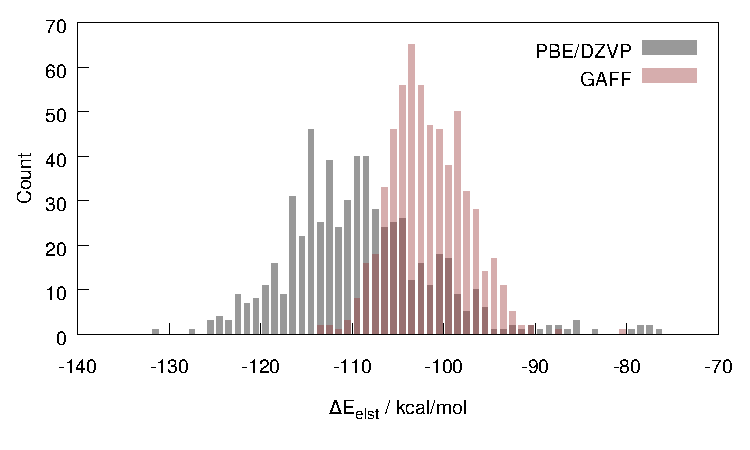
\includegraphics[width=0.9\linewidth]{images/ecpc/liec_elst.pdf} \\
 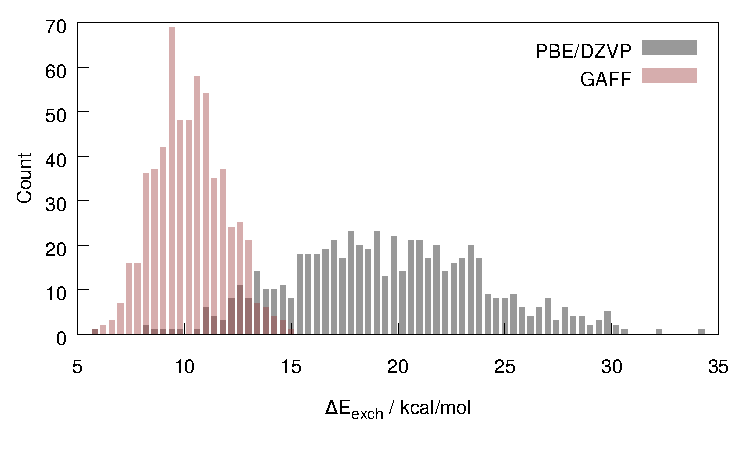
\includegraphics[width=0.9\linewidth]{images/ecpc/liec_exch.pdf}
 \end{center} 
 \caption[SAPT(KS)-D3 electrostatic and exchange energies of (LiEC\sous{4})\sur{+}]{\label{fig:ecsapt1}SAPT(KS)-D3 electrostatic (top) and exchange (bottom)
 energies of (LiEC\sous{4})\sur{+}. All energies in kcal/mol.}
\end{figure}

\begin{figure}
 \begin{center}
 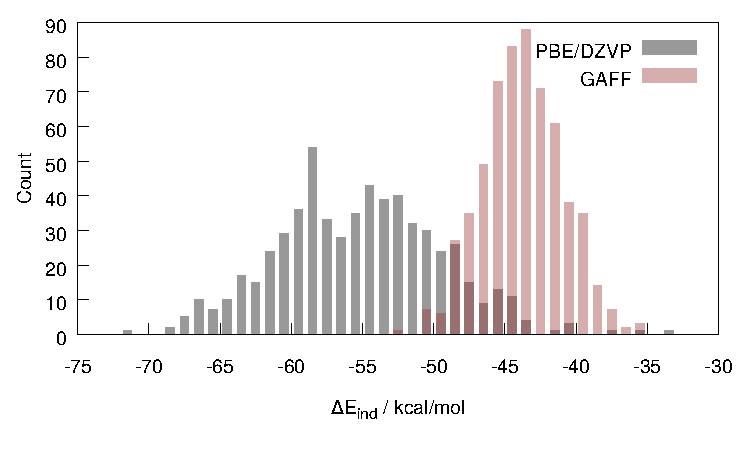
\includegraphics[width=0.9\linewidth]{images/ecpc/liec_ind.pdf} \\
 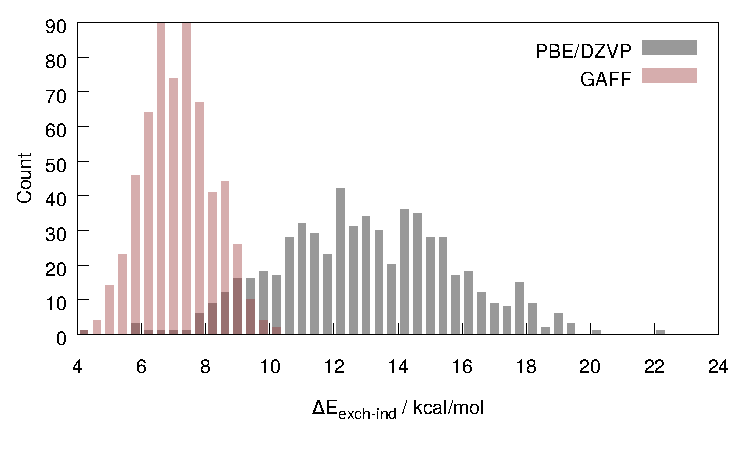
\includegraphics[width=0.9\linewidth]{images/ecpc/liec_exch-ind.pdf}
 \end{center} 
 \caption[SAPT(KS)-D3 induction and exchange-induction energies of (LiEC\sous{4})\sur{+}]{\label{fig:ecsapt2}SAPT(KS)-D3 induction (top) and exchange-induction
 (bottom) energies of (LiEC\sous{4})\sur{+}. All energies in kcal/mol.}
\end{figure}

\begin{figure}
 \begin{center}
 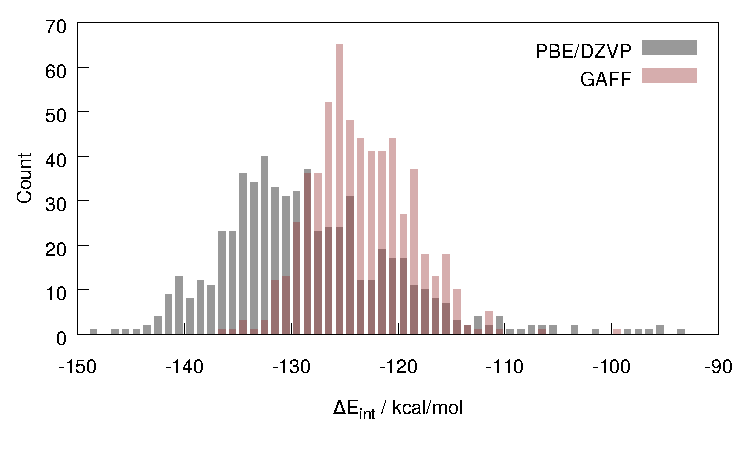
\includegraphics[width=0.9\linewidth]{images/ecpc/liec_int.pdf}
 \end{center} 
 \caption[SAPT(KS)-D3 interaction energies of (LiEC\sous{4})\sur{+}]{\label{fig:ecsaptint}SAPT(KS)-D3 interaction energies of (LiEC\sous{4})\sur{+} with dispersion and
 $\delta_{HF}^{(2)}$ included. All energies in kcal/mol.}
\end{figure}

\begin{figure}
 \begin{center}
 \includegraphics[width=0.9\linewidth]{images/ecpc/lipc_elst.pdf} \\
 \includegraphics[width=0.9\linewidth]{images/ecpc/lipc_exch.pdf}
 \end{center} 
 \caption[SAPT(KS)-D3 electrostatic and exchange energies of (LiPC\sous{4})\sur{+}]{\label{fig:pcsapt1}SAPT(KS)-D3 electrostatic (top) and exchange (bottom)
 energies of (LiPC\sous{4})\sur{+}. All energies in kcal/mol.}
\end{figure}

\begin{figure}
 \begin{center}
 \includegraphics[width=0.9\linewidth]{images/ecpc/lipc_ind.pdf} \\
 \includegraphics[width=0.9\linewidth]{images/ecpc/lipc_exch-ind.pdf}
 \end{center} 
 \caption[SAPT(KS)-D3 induction and exchange-induction energies of (LiPC\sous{4})\sur{+}]{\label{fig:pcsapt2}SAPT(KS)-D3 induction (top) and exchange-induction
 (bottom) energies of (LiPC\sous{4})\sur{+}. All energies in kcal/mol.}
\end{figure}

\begin{figure}
 \begin{center}
 \includegraphics[width=0.9\linewidth]{images/ecpc/lipc_int.pdf}
 \end{center} 
 \caption[SAPT(KS)-D3 interaction energies of (LiPC\sous{4})\sur{+}]{\label{fig:pcsaptint}SAPT(KS)-D3 interaction energies of (LiPC\sous{4})\sur{+} with dispersion and
 $\delta_{HF}^{(2)}$ included. All energies in kcal/mol.}
\end{figure} 
 \chapter{Quasichemical partitions of the solvation free energies~}
\label{chap:a6}

\copypagestyle{chapter}{plain}
\makeoddfoot{chapter}{}{}{}
\makeevenhead{chapter}{\thepage}{}{}
\makeoddhead{chapter}{}{}{\thepage}

Document presents tables of all the single-ion free energy components (and errors) and totals on both the intrinsic and bulk free energy scales for water, DMSO, 
and 1,2-DCE. All units are kcal/mol. Packing and local potential with errors are listed in the caption for each table. The mean-field and third order contributions 
to the local potential are also reported. These data were used to generate several of the figures in the main text.

\begin{table}
 \begin{center}
 \begin{tabular}{ccccc}
  \hline
  \hline
   Ion &   $\mu\sursous{ex}{is}$  &   $\mu\sursous{ex}{os}$  &   $\mu\sursous{ex}{int}$  &   $\mu\sursous{ex}{b}$  \\
  \hline
ak	&	105.67	$\pm$	0.59	&	13.68	$\pm$	0.10	&	-36.58	$\pm$	0.87	&	-45.53	$\pm$	0.88	\\
bl	&	91.64	$\pm$	0.62	&	14.13	$\pm$	0.14	&	-23.00	$\pm$	0.89	&	-31.95	$\pm$	0.91	\\
cm	&	87.32	$\pm$	0.68	&	14.61	$\pm$	0.14	&	-19.16	$\pm$	0.94	&	-28.11	$\pm$	0.95	\\
dn	&	81.47	$\pm$	0.61	&	15.11	$\pm$	0.12	&	-13.81	$\pm$	0.89	&	-22.76	$\pm$	0.90	\\
eo	&	76.98	$\pm$	0.57	&	15.43	$\pm$	0.12	&	-9.64	$\pm$	0.86	&	-18.59	$\pm$	0.87	\\
fp	&	103.53	$\pm$	0.69	&	14.53	$\pm$	0.16	&	-35.29	$\pm$	0.95	&	-44.24	$\pm$	0.96	\\
gq	&	92.90	$\pm$	0.65	&	16.17	$\pm$	0.13	&	-26.30	$\pm$	0.91	&	-35.25	$\pm$	0.93	\\
hr	&	87.50	$\pm$	0.56	&	17.38	$\pm$	0.14	&	-22.11	$\pm$	0.85	&	-31.06	$\pm$	0.87	\\
is	&	83.68	$\pm$	0.60	&	18.73	$\pm$	0.15	&	-19.64	$\pm$	0.88	&	-28.59	$\pm$	0.89	\\
jt	&	78.36	$\pm$	0.60	&	20.41	$\pm$	0.17	&	-16.00	$\pm$	0.89	&	-24.95	$\pm$	0.90	\\
ka	&	117.97	$\pm$	0.65	&	31.72	$\pm$	0.12	&	-66.92	$\pm$	0.91	&	-57.97	$\pm$	0.92	\\
lb	&	100.01	$\pm$	0.54	&	32.18	$\pm$	0.13	&	-49.42	$\pm$	0.84	&	-40.47	$\pm$	0.85	\\
mc	&	92.23	$\pm$	0.60	&	32.57	$\pm$	0.16	&	-42.03	$\pm$	0.88	&	-33.08	$\pm$	0.90	\\
nd	&	85.54	$\pm$	0.54	&	32.98	$\pm$	0.16	&	-35.75	$\pm$	0.85	&	-26.80	$\pm$	0.86	\\
oe	&	80.20	$\pm$	0.54	&	33.56	$\pm$	0.20	&	-30.99	$\pm$	0.85	&	-22.04	$\pm$	0.86	\\
pf	&	114.17	$\pm$	0.59	&	32.52	$\pm$	0.12	&	-63.92	$\pm$	0.87	&	-54.97	$\pm$	0.88	\\
qg	&	97.52	$\pm$	0.59	&	34.06	$\pm$	0.17	&	-48.81	$\pm$	0.88	&	-39.86	$\pm$	0.89	\\
rh	&	90.25	$\pm$	0.48	&	35.15	$\pm$	0.17	&	-42.63	$\pm$	0.81	&	-33.68	$\pm$	0.82	\\
si	&	86.14	$\pm$	0.54	&	36.55	$\pm$	0.16	&	-39.92	$\pm$	0.85	&	-30.97	$\pm$	0.86	\\
tj	&	80.59	$\pm$	0.50	&	38.21	$\pm$	0.12	&	-36.03	$\pm$	0.81	&	-27.08	$\pm$	0.83	\\
  \hline
  \hline
 \end{tabular}
 \end{center}
 \caption[Quasichemical partitioning of solvation free energies in water]{\label{tab:wat}Single-ion free energies of all ions in SPC/E water using the QCT method. 
 Ion labels are as they were given in the main text. By column, 
 we report inner shell, outer shell, intrinsic, and bulk free energy quantities all in kcal/mol. The intrinsic free energy is the resultant sum of the inner and 
 outer shell figures and also includes the packing term evaluated as 82.77 $\pm$ 0.63 kcal/mol. Bulk free energy quantities differ only by inclusion of a 
 -q$\phi\sous{lp}$ term  for the local potential, where q is the ion charge and $\phi\sous{lp}$ was determined to be 8.95 $\pm$ 0.14 kcal/mol-e at the center of 
 a 0.9 nm radius cavity. $\phi\sous{lp}$ is constructed from the sum of the first and third cumulants which are 8.76 kcal/mol-e and 0.20 kcal/mol-e, respectively.}
\end{table}

\begin{table}
 \begin{center}
 \begin{tabular}{ccccc}
  \hline
  \hline
   Ion &   $\mu\sursous{ex}{is}$  &   $\mu\sursous{ex}{os}$  &   $\mu\sursous{ex}{int}$  &   $\mu\sursous{ex}{b}$  \\
  \hline
ak	&	114.18	$\pm$	0.98	&	12.81	$\pm$	0.29	&	-43.49	$\pm$	1.37	&	-49.93	$\pm$	1.39	\\
bl	&	99.71	$\pm$	0.93	&	13.54	$\pm$	0.26	&	-29.75	$\pm$	1.33	&	-36.19	$\pm$	1.35	\\
cm	&	92.29	$\pm$	0.84	&	13.81	$\pm$	0.29	&	-22.60	$\pm$	1.27	&	-29.04	$\pm$	1.29	\\
dn	&	89.50	$\pm$	0.92	&	14.55	$\pm$	0.16	&	-20.55	$\pm$	1.30	&	-26.99	$\pm$	1.33	\\
eo	&	82.42	$\pm$	0.74	&	15.23	$\pm$	0.27	&	-14.15	$\pm$	1.20	&	-20.59	$\pm$	1.23	\\
fp	&	116.12	$\pm$	0.98	&	13.71	$\pm$	0.34	&	-46.33	$\pm$	1.38	&	-52.77	$\pm$	1.40	\\
gq	&	105.20	$\pm$	0.95	&	15.86	$\pm$	0.33	&	-37.56	$\pm$	1.36	&	-44.00	$\pm$	1.38	\\
hr	&	99.80	$\pm$	0.89	&	17.22	$\pm$	0.29	&	-33.52	$\pm$	1.31	&	-39.96	$\pm$	1.33	\\
is	&	95.24	$\pm$	0.84	&	19.31	$\pm$	0.28	&	-31.05	$\pm$	1.27	&	-37.49	$\pm$	1.29	\\
jt	&	91.12	$\pm$	0.77	&	21.60	$\pm$	0.27	&	-29.22	$\pm$	1.22	&	-35.66	$\pm$	1.25	\\
ka	&	103.76	$\pm$	1.08	&	28.59	$\pm$	0.30	&	-48.85	$\pm$	1.44	&	-42.42	$\pm$	1.46	\\
lb	&	92.51	$\pm$	0.95	&	29.12	$\pm$	0.27	&	-38.13	$\pm$	1.34	&	-31.70	$\pm$	1.36	\\
mc	&	88.31	$\pm$	0.92	&	29.54	$\pm$	0.34	&	-34.35	$\pm$	1.34	&	-27.92	$\pm$	1.36	\\
nd	&	84.75	$\pm$	0.94	&	30.01	$\pm$	0.25	&	-31.26	$\pm$	1.33	&	-24.83	$\pm$	1.35	\\
oe	&	81.09	$\pm$	0.81	&	30.72	$\pm$	0.31	&	-28.31	$\pm$	1.26	&	-21.88	$\pm$	1.28	\\
pf	&	107.46	$\pm$	0.97	&	29.47	$\pm$	0.25	&	-53.43	$\pm$	1.35	&	-47.00	$\pm$	1.37	\\
qg	&	99.60	$\pm$	0.84	&	31.25	$\pm$	0.27	&	-47.35	$\pm$	1.27	&	-40.92	$\pm$	1.29	\\
rh	&	97.73	$\pm$	0.81	&	32.60	$\pm$	0.29	&	-46.83	$\pm$	1.25	&	-40.40	$\pm$	1.28	\\
si	&	92.58	$\pm$	0.88	&	34.30	$\pm$	0.26	&	-43.38	$\pm$	1.29	&	-36.95	$\pm$	1.31	\\
tj	&	89.52	$\pm$	0.80	&	36.28	$\pm$	0.27	&	-42.30	$\pm$	1.24	&	-35.87	$\pm$	1.26	\\
  \hline
  \hline
 \end{tabular}
 \end{center}
 \caption[Quasichemical partitioning of solvation free energies in dimethyl sulfoxide]{\label{tab:dmso}Single-ion free energies of all ions in OPLS/AA dimethyl
 sulfoxide using the QCT method. Ion labels are as they were given in the main text.
 By column, we report inner shell, outer shell, intrinsic, and bulk free energy quantities all in kcal/mol. The intrinsic free energy is the resultant sum of the inner
 and outer shell figures and also includes the packing term evaluated as 83.50 $\pm$ 0.91 kcal/mol. Bulk free energy quantities differ only by inclusion of a 
 -q$\phi\sous{lp}$ term  for the local potential, where q is the ion charge and $\phi\sous{lp}$ was determined to be 6.44 $\pm$ 0.24 kcal/mol-e at the center of 
 a 0.9 nm radius cavity. $\phi\sous{lp}$ is constructed from the sum of the first and third cumulants which are 6.71 kcal/mol-e and -0.27 kcal/mol-e, respectively.}
\end{table}

\begin{table}
 \begin{center}
 \begin{tabular}{ccccc}
  \hline
  \hline
   Ion &   $\mu\sursous{ex}{is}$  &   $\mu\sursous{ex}{os}$  &   $\mu\sursous{ex}{int}$  &   $\mu\sursous{ex}{b}$  \\
  \hline
ak	&	68.01	$\pm$	0.59	&	21.18	$\pm$	0.23	&	-39.74	$\pm$	0.85	&	-38.48	$\pm$	0.87	\\
bl	&	58.45	$\pm$	0.56	&	21.81	$\pm$	0.19	&	-30.81	$\pm$	0.81	&	-29.55	$\pm$	0.84	\\
cm	&	54.10	$\pm$	0.54	&	22.16	$\pm$	0.24	&	-26.81	$\pm$	0.81	&	-25.55	$\pm$	0.84	\\
dn	&	50.20	$\pm$	0.53	&	22.68	$\pm$	0.26	&	-23.43	$\pm$	0.81	&	-22.17	$\pm$	0.84	\\
eo	&	47.82	$\pm$	0.49	&	23.32	$\pm$	0.21	&	-21.69	$\pm$	0.77	&	-20.43	$\pm$	0.80	\\
fp	&	69.68	$\pm$	0.59	&	22.09	$\pm$	0.21	&	-42.32	$\pm$	0.84	&	-41.06	$\pm$	0.86	\\
gq	&	62.32	$\pm$	0.53	&	23.72	$\pm$	0.20	&	-36.59	$\pm$	0.80	&	-35.33	$\pm$	0.82	\\
hr	&	58.77	$\pm$	0.59	&	25.03	$\pm$	0.25	&	-34.35	$\pm$	0.85	&	-33.09	$\pm$	0.87	\\
is	&	54.98	$\pm$	0.57	&	26.37	$\pm$	0.23	&	-31.90	$\pm$	0.83	&	-30.64	$\pm$	0.86	\\
jt	&	52.90	$\pm$	0.54	&	28.28	$\pm$	0.24	&	-31.73	$\pm$	0.81	&	-30.47	$\pm$	0.84	\\
ka	&	77.56	$\pm$	0.66	&	18.14	$\pm$	0.17	&	-46.25	$\pm$	0.88	&	-47.51	$\pm$	0.90	\\
lb	&	68.29	$\pm$	0.60	&	18.58	$\pm$	0.22	&	-37.42	$\pm$	0.85	&	-38.68	$\pm$	0.87	\\
mc	&	63.22	$\pm$	0.60	&	18.94	$\pm$	0.23	&	-32.71	$\pm$	0.85	&	-33.97	$\pm$	0.88	\\
nd	&	59.94	$\pm$	0.60	&	19.34	$\pm$	0.20	&	-29.83	$\pm$	0.84	&	-31.09	$\pm$	0.87	\\
oe	&	56.13	$\pm$	0.54	&	20.01	$\pm$	0.25	&	-26.69	$\pm$	0.82	&	-27.95	$\pm$	0.84	\\
pf	&	80.16	$\pm$	0.71	&	18.89	$\pm$	0.19	&	-49.60	$\pm$	0.92	&	-50.86	$\pm$	0.95	\\
qg	&	73.20	$\pm$	0.63	&	20.39	$\pm$	0.14	&	-44.14	$\pm$	0.85	&	-45.40	$\pm$	0.88	\\
rh	&	69.55	$\pm$	0.60	&	21.47	$\pm$	0.20	&	-41.57	$\pm$	0.84	&	-42.83	$\pm$	0.87	\\
si	&	65.77	$\pm$	0.64	&	22.80	$\pm$	0.23	&	-39.12	$\pm$	0.88	&	-40.38	$\pm$	0.90	\\
tj	&	62.63	$\pm$	0.56	&	24.50	$\pm$	0.25	&	-37.68	$\pm$	0.83	&	-38.94	$\pm$	0.85	\\
  \hline
  \hline
 \end{tabular}
 \end{center}
 \caption[Quasichemical partitioning of solvation free energies in 1,2-dichloroethane]{\label{tab:dce}Single-ion free energies of all ions in OPLS-AA 
 1,2-dichloroethane using the QCT method. Ion labels are as they were given in the main text.
 By column, we report inner shell, outer shell, intrinsic, and bulk free energy quantities in kcal/mol. The intrinsic free energy is the resultant sum of the inner 
 and outer shell figures and also includes the packing term evaluated as 49.45 $\pm$ 0.56 kcal/mol. Bulk free energy quantities differ only by inclusion of a 
 -q$\phi\sous{lp}$ term for the local potential, where q is the ion charge and $\phi\sous{lp}$ was determined to be -1.26 $\pm$ 0.20 kcal/mol-e at the center of a 
 0.9 nm radius cavity. $\phi\sous{lp}$ is constructed from the sum of the first and third cumulants which are -1.42 kcal/mol-e and 0.16 kcal/mol-e, respectively.}
\end{table} 
 \end{appendices}

%% Are you a big nerd with a colophon?  Add it here.
%\begin{colophon}
%\svnidlong{$LastChangedBy$}{$LastChangedRevision$}{$LastChangedDate$}{$HeadURL: http://freevariable.com/dissertation/trunk/frontmatter.tex $}
\vcinfo{}



%\end{colophon}

%% McBride is a very nice style (some version is included in this distribution)
\separatorpage{Intentionally left blank}
\restoregeometry
\clearpage
\copypagestyle{chapter}{plain}
\makeoddfoot{chapter}{}{}{}
\makeevenhead{chapter}{\thepage}{}{}
\makeoddhead{chapter}{}{}{\thepage}
\part{~References}
\renewcommand\bibname{List of references~}
\bibliographystyle{abbrv}
\bibliography{bib/thesis_univ}

%% Want an index?  Neither did I.
%\printindex

\end{document}
